%Définition des différents répertoires à prendre à compte
\makeatletter\def\input@path{
{/media/MYWIN7OS/swp55/Docs0512/PhysQuant/}
% {/media/MYWIN7OS/swp55/Docs0512/MIL4AR08New/}
}\makeatother
%
\documentclass[12pt,a4paper,oneside,openany]{book}%
\usepackage{graphicx,amsmath,amsfonts,amssymb,cclicenses}
% Box pour titres gestion des entêtes et pieds de pages
\usepackage{fancybox,fancyhdr}
%Gestion de la présentation des titres des chapitres
\usepackage[Glenn]{fncychap}
% Gestion de la langue française et de l'encodage
\usepackage[french]{babel}
\usepackage[utf8]{inputenc}
\usepackage[T1]{fontenc}
% Gestion de la page (mode économique)
\usepackage[a4paper,includeheadfoot,compat2]{geometry}
%
\usepackage{color,colortbl,array,lmodern}
\usepackage{multicol,wrapfig}
% Écriture des algorithmes
\usepackage{algpseudocode} % Codes semblables à fortran ou pascal ou C
\usepackage[section]{algorithm}
%
\usepackage[bf,textfont={small,it}]{caption}
\usepackage[toc,page,title,titletoc,header]{appendix}
\usepackage[Glenn]{fncychap}
% Pour générer une mini-table de matière au début de chaque chapitre et dans
%une boite
\usepackage[french]{minitoc-hyper}
\usepackage{myminitoc,titlebox}
% Gestion des liens hypertextes
\usepackage[colorlinks,linkcolor=black,citecolor=black,urlcolor=black]{hyperref}
%
% Prise en compte du langage Python
\usepackage{listings}
\lstset{
language=Python,
basicstyle=\footnotesize,
numbers=left,
numberstyle=\footnotesize,
numbersep=5pt,
backgroundcolor=\color[gray]{.95},
mathescape=true,
numberblanklines=false,
numberbychapter=true
escapechar=\%
}
% Gestion du fichier pdf
\hypersetup{%
   bookmarksnumbered=true,%
   pdfauthor=Nana Engo,
   pdfsubject={Uni Ndéré, Fac Sciences, MIL4R08-MIL4CS07},%
   pdfkeywords={Qubits, Amplitude de probabilité, Opérateurs, Cryptographie et
Téléportation quantiques, Portes et Circuits quantiques},%
   pdftitle=Introduction à l'Information Quantique V13.05%
}
\setcounter{MaxMatrixCols}{30}
\setlength{\abovecaptionskip}{0pt}
\setlength{\belowcaptionskip}{0pt}
\newtheorem{theorem}{Théorème}[section]
\newtheorem{acknowledgement}{Remerciements}
\newtheorem{example}{Exemple}[section]
\newtheorem{exercise}{Exercice}[section]
\newtheorem{problem}{Problème}[section]
\newtheorem{remark}{Remarque}[section]
\newtheorem{proposition}{Proposition}[section]
\newtheorem{conclusion}{Conclusion}[section]
\newtheorem{principe}{Principe}[section]
\newtheorem{definition}{Définition}[section]
%\newtheorem{algorithm}{Algorithme}[section]
\newtheorem{solution}{Solution}[section]
\newenvironment{proof}[1][Preuve]{\noindent\textbf{#1.} }{\ \rule{0.5em}{0.5em}}
% Numérotations à deux chiffres des sections, figures et tableaux
\numberwithin{equation}{section}
\numberwithin{figure}{section}
\numberwithin{table}{section}
\frenchbsetup{StandardLayout}
% Commandes pour les unités et vecteurs en gras
\newcommand{\opn}[1]{\ensuremath{\operatorname{#1}}} % Operatorname
\newcommand{\bls}[1]{\ensuremath{\boldsymbol{#1}}} %Boldsymbol
\newcommand{\av}[1]{\langle{#1}\rangle} %Average
%
\pagestyle{fancy}
\fancyhf{}
\fancyhead[RE]{\textsl{\leftmark}}
\fancyhead[LO]{\textsl{\rightmark}}
\fancyhead[LE,RO]{\thepage}
\fancyfoot[LE,RO]{V13.04}
% \fancyfoot[LO,RE]{\footnotesize Copyright \copyright \! Nana Engo}
\fancyfoot[LO,RE]{\tiny\copyright \! Nana Engo - Sous la licence \cc \bysa 3.0}
\fancyfoot[CO,CE]{\tiny{\emph{INTRO A L'INFORMATION QUANTIQUE}}}
\renewcommand{\footrulewidth}{0.4pt}
%BeginMSIPreambleData
\ifx\pdfoutput\relax\let\pdfoutput=\undefined\fi
\newcount\msipdfoutput
\ifx\pdfoutput\undefined\else
\ifcase\pdfoutput\else
\msipdfoutput=1
\ifx\paperwidth\undefined\else
\ifdim\paperheight=0pt\relax\else\pdfpageheight\paperheight\fi
\ifdim\paperwidth=0pt\relax\else\pdfpagewidth\paperwidth\fi
\fi\fi\fi
%EndMSIPreambleData
\input{Qcircuit}
%
\begin{document}
\frontmatter
\begin{titlepage}
\begin{small}
\begin{center}
 \begin{tabular}[h]{l}
  UNIVERSITÉ DE NGAOUNDÉRÉ \\FACULTÉ DES SCIENCES
 \end{tabular}
\hspace*{2em}
\begin{minipage}{2cm}

\includegraphics[width = 1.6cm]{graphics/LogoUN.png}
\end{minipage}
\hspace*{1em}
\begin{tabular}[h]{r}
  \\MATHS - INFORMATIQUE\\LICENCE DE MATHS-INFO
 \end{tabular}
\end{center}
\end{small}
\vspace*{5em}
\begin{center}
\color{black}\rule{14.75cm}{0.09cm}\color{black}
\bigskip

{\Huge INTRODUCTION A L'INFORMATION QUANTIQUE}

\color{black}\rule{12.55cm}{0.09cm}\color{black}

\vspace*{2em}

MIL4AR08/CS07 - UE Optionnelle\\ CM: 30h - TD: 20h - Crédits: 5\\

 \vspace*{5em}
{\Large \textbf{NANA ENGO}}\vspace*{3em}
\begin{center}
\begin{tabular}{c}
\Qcircuit @C=1em @R=1.em {
&\mbox{EPR}\\
\lstick{\alpha\ket{0}+\beta\ket{1}} & \ctrl{1} & \qw      & \qw      & \qw
&  \qw     & \qw        & \qw      & \qw      & \qw      & \qw      & \qw
& \ctrl{3} & \targ     & \qw \\
\lstick{\ket{1}} 		    & \targ    & \qw      & \qw      & \gate{W}
& \ctrl{1} & \gate{W}  & \qw      & \ctrl{2} & \qw      & \qw      & \qw       &
\qw      & \qw       & \qw \\
\lstick{\ket{0}} 		    & \gate{W}& \ctrl{1} & \ctrl{2} & \qw
& \targ    & \ctrl{1}   & \qw      & \qw      & \qw      & \ctrl{2} & \qw
& \qw      & \qw       & \qw \\
\lstick{\ket{0}}    		    & \qw      & \targ    & \qw      & \qw
& \qw      & \targ      & \gate{W}& \targ    & \gate{W}& \qw      & \targ     &
\targ    & \qw       & \qw \\
\lstick{\ket{0}}    		    & \qw      & \qw      & \targ    & \qw
& \qw      & \qw        & \qw      & \qw      & \qw      & \targ    & \ctrl{-1}
& \gate{W}& \ctrl{-4} & \qw \\
&&\mbox{{GHZ}}&&&&&\mbox{Téléportation d'une pair EPR}
\gategroup{2}{2}{3}{2}{.7em}{--}\gategroup{4}{2}{6}{4}{.7em}{--}
}
\end{tabular}
\end{center}

\vspace*{5cm}
{\small \textbf{\emph{Année académique}} $2012-2013$ \\ Copyright ©\! 
 Nana Engo - Sous la licence \cc \bysa 3.0}
\end{center}

\end{titlepage}
\tableofcontents

\chapter{Avant-propos}

\markboth{Avant-Propos}{Avant-Propos} Cette unité d'enseignement (UE) a pour
objectif d'exposer aux étudiants du cycle Licence des Mentions Mathématique et
Informatique, les notions de base de la théorie quantique nécessaires à la
compréhension de l'information quantique. Laquelle permet de traiter et
transmettre l'information en s'appuyant sur les spécificités de la théorie
quantique.

Les progrès des techniques et de la connaissance permettent aujourd'hui
d'agencer de façon contrôlée un petit nombre d'atomes pour fabriquer des
objets de taille nanométrique\footnote{Le millionième de millimètre!} qui
présentent des propriétés extraordinaires, d'origine quantique, qui sont
exploitées dans la quasi-totalité des domaines industriels.

En effet, le monde de l'information dans lequel nous vivons aujourd'hui résulte
de la synergie entre l'informatique et la théorie quantique à travers
l'invention du transistor. Cependant, l'ultra-miniaturisation croissante des
composants électronique, suit deux lois émise en 1965 par Gordon Moore,
co-fondateur de la société INTEL:
\begin{itemize}
  \item\textbf{1ère loi de Moore:} \emph{tous les dix-huit mois, la complexité
et les performances (rendement technologique) des circuits seront multipliées
par deux};
  \item\textbf{2ème loi de Moore:} \emph{à chaque génération le coût des
équipements de fabrication sera multiplié par deux}.
\end{itemize}

En vertu de la 1ère loi,
\begin{itemize}
  \item L'augmentation du nombre de connexions limite les possibilités
d'intégration sur une puce;
  \item La réduction du temps de calcul est limitée par les délais de
commutations entre transistors;
  \item Le nombre important de composants sur une même puce entraîne \emph{ipso
facto} une augmentation de la consommation électrique, et par voie de
conséquent, à travers la loi de Ohm, celle de la quantité de chaleur dissipée
dans la puce.
\end{itemize}

\begin{figure}[ptbh]
\centering
  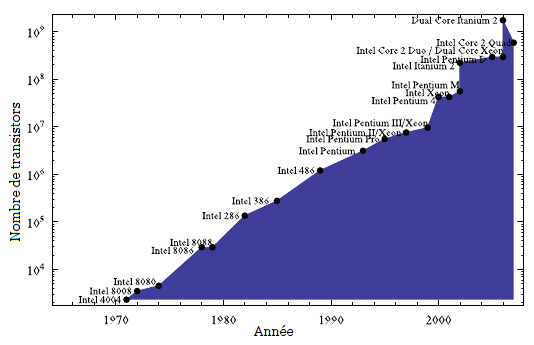
\includegraphics{graphics/LoiMoore.png}
\caption{Depuis quatre décennies, la densité des transistors réalisés sur une
même puce double tous les dix-huit mois.}
\label{fig:LoiMoore}
\end{figure}

Ainsi comme on peut le voir sur la figure \ref{fig:LoiMoore}, par rapport aux
nombre de connexions, d'ici 2020 le bit d'information sera stocké sur une puce
de dimension atomique. Et alors, les effets quantiques commenceront à être
prédominants. Les électrons jusque là bien ordonnés révéleront leur nature
quantique, qui est, entre autres, probabiliste. Les transistors pourraient
ainsi, ne plus être de manière déterministe dans l'état ON ou OFF, mais se
retrouver dans une superposition des deux, avec une certaine probabilité d'être
dans l'état ON ou dans l'état OFF. Un tel comportement n'appelle aucune
alternative: il faudra soit adapter l'architecture des ordinateurs pour
minimiser les nuisances occasionnées par les effets quantiques, ou alors changer
radicalement d'architecture en ouvrant les bras à ces effets quantiques.
L'information quantique suit cette deuxième approche.

Mais hormis ces effets quantiques, les considérations économiques, que met en
évidence la 2ème loi de Moore, vont aussi rendre inopérants la 1ère loi de
Moore. En effet, pour réduire les coûts de fabrication, on pense de plus en plus
à l'\textbf{auto-assemblage} des composants. Celui-ci est possible depuis le
début des années 1980 par \emph{la capacité des physiciens à manipuler et
observer des objets quantiques élémentaires individuels}: atomes, photons,
électrons, etc. Il est à noter que c'est l'auto-assemblage que suit la vie en
pratiquant l'assemblage des molécules pour créer les protéines, enchaînement
d'acides aminés, que de super-molécules, les acides nucléiques (ARN, ADN),
savent faire produire au sein de cellules pour former des organismes, les faire
fonctionner et se reproduire tout en se complexifiant. Cette voie, dite
\emph{\textbf{bottom-up}}, vise à organiser la matière à partir des
\emph{briques de base}, dont les atomes eux-mêmes sont les plus petits
constituants, à l'instar du monde vivant. La nanoélectronique du futur cherche à
emprunter cette voie d'assemblage pour aboutir à moindre coût à la fabrication
d'éléments fonctionnels, puisque \textbf{la technologie ne progresse qu'en
devenant moins chère!}

Grâce à l'information quantique, on peut par exemple concevoir de nouvelles
méthodes de cryptographie dont la sécurité s'appuie sur les bases du formalisme
quantique, ou de nouvelles méthodes de calculs qui peuvent être 
exponentiellement plus efficaces que les méthodes classiques. L'information
quantique ne concerne donc pas seulement les physiciens, mais aussi les
théoriciens de l'information, les algorithmiciens, et les mathématiciens
travaillant sur la théorie de la complexité.

Ces notes de cours sont volontairement très détaillées et enrichies de nombreux
exemples afin de palier à la carence d'ouvrages appropriés dans l'environnement
actuel de l'étudiant de la Faculté des Sciences de l'Université de Ngaoundéré.

Le contenu du cours est le suivant:

\begin{itemize}
\item \textbf{Chapitre I: Qubits et états quantiques}

Qubit ou bit quantique et espace de Hilbert. Phénomènes quantiques (Interférence
à une particule). Vecteurs d'état et amplitudes de probabilité. Règles de calcul
des amplitudes de probabilité.

\item \textbf{Chapitre II: Mesure et opérateurs linéaires}

Mesure de grandeurs physiques et opérateurs. Opérateurs linéaires et
représentation matricielle. Diagonalisation d'un opérateur hermitien. Ensemble
complet d'opérateurs qui commutent (ECOC).

\item \textbf{Chapitre III: Postulats et évolution temporelle}

Postulats de la théorie quantique. Évolution temporelle. Inégalités
d'Heisenberg. Manipulations des qubits: oscillations de Rabi.

\item \textbf{Chapitre IV: Corrélations quantiques}

Produit tensoriel. Interférences des états corrélés. Analyse EPR et inégalités
de Bell. Non-clonage quantique. Cryptographie quantique. Téléportation
quantique.

\item \textbf{Chapitre V: Calculs quantiques}

Calculs réversibles. Portes logiques et circuits quantiques. Bases de Bell.
Algorithme de Deutsch-Jozsa. Transformation de Fourier quantique.
\end{itemize}

\mainmatter
%
%\input{test}


\chapter{Qubits et états quantiques}
\label{sec:AmplProb}
\minitoc

\bigskip


Dans ce chapitre nous présentons le cadre général de la théorie quantique en
utilisant la puissante et élégante algèbre de Dirac. La \textbf{section
\ref{sec:Inter1Part}} est consacrée à la découverte de l'étrange monde quantique
à travers quelques expériences d'interférences à une particule. Ces expériences
montrent que l'intuition et le \emph{bon sens} hérités de la physique classique
sont inadaptés dans le monde quantique du fait de la nature fondamentalement
\textbf{probabiliste} ou \textbf{indéterministe} des phénomènes quantiques.
Cette nature impose l'introduction, à la \textbf{section \ref{sec:AmplProba}},
des concepts nouveaux et essentiels d'état quantique, d'amplitude de probabilité
ou amplitude de transition, de superposition d'état ou \textbf{qubit} et de
l'espace de Hilbert. Ces concepts ont été auparavant présenté de façon
\emph{mathématique} à la \textbf{section \ref{sec:qbit}}.

\section{Qubit ou bit quantique et espace de Hilbert}
\label{sec:qbit}

\subsection{Qubit ou bit quantique}

L'unité fondamentale de l'informatique classique est le bit (de l'anglais
\emph{binary digit}). Un bit peut prendre deux valeurs que l'on note
habituellement $0$ et $1$. Évidemment, ce choix de notation, complètement
arbitraire, n'est que la représentation symbolique du stockage du bit dans un
système à deux états. En effet, la valeur $0$ d'un bit peut être représentée
physiquement dans un ordinateur par un condensateur non chargé et la valeur $1$,
représentée par le même condensateur chargé (voir la figure
\ref{fig:CodageClas}). La différence entre les deux états (chargé et non chargé)
se traduit par le déplacement de plusieurs millions d'électrons. Ainsi, un bit
d'information classique implique environ $10^{9}$ électrons dans la mémoire vive
d'un ordinateur. Il s'agit donc d'un comportement \emph{collectif}.

\begin{figure}[ptbh]
\centering
\ifcase\msipdfoutput
  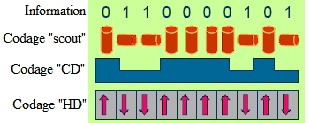
\includegraphics[scale=1]{graphics/CodageClas.jpg}
\else
  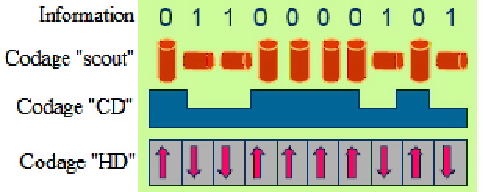
\includegraphics[scale=1]{graphics/CodageClas.pdf}
\fi
\caption{\textbf{Codage classique}. L'information, que l'on représente par les
\textbf{bits} $0$ et $1$, est toujours codée dans des systèmes physiques
bistables.}
\label{fig:CodageClas}%
\end{figure}

\begin{figure}[ptbh]
\centering
  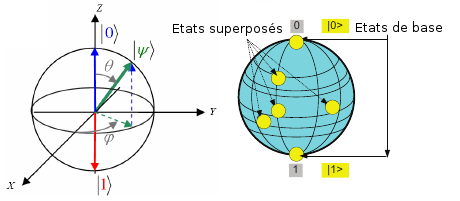
\includegraphics[scale=1]{graphics/SphereBloch.png}%
\caption{\textbf{Codage quantique.} Le qubit $\ket{\psi} =\alpha\ket{0}
+\beta\ket{1}$ (avec $\alpha=\cos\frac{\theta}{2},
\beta=e^{i\varphi}\sin\frac{\theta}{2}$ et $|\alpha|^{2}+|\beta|^{2}=1$), offre
une description différente des systèmes physiques. Les états binaires classiques
sont aux pôles de la sphère. Il opère dans un univers multidimensionnel, ces
états propres correspondant à la surface de la sphère, alors que les états
logiques classiques correspondent aux pôles de cette sphère.}
\label{fig:SphereBloch}
\end{figure}

L'unité fondamentale de l'information quantique est le bit quantique ou, plus
simplement, \textbf{qubit} (de l'anglais \emph{quantum bit}). Il est
superficiellement similaire au bit classique, mais comme nous le ferons, il est
fondamentalement différent et cette différence fondamentale permet le
traitement de l'information de façons nouvelles et très prometteuses.

Comme le bit, le qubit peut-être dans un des états $0$ ou $1$. Pour une raison
qu'on expliquera ci-dessous, on notera ces états $\ket{0}$ et $\ket{1}$ et on
lira \textbf{\emph{ket de 0}} et \textbf{\emph{ket de 1}}. Cette notation est
appelée \textbf{notation de Dirac} et représente un \emph{vecteur d'état} ou
un \emph{état} tout simplement.

A la différence du bit classique, le qubit peut-être \textbf{à la fois} dans
l'état $\ket{0}$ et  $\ket{1}$. On dit alors qu'il est dans \textbf{état
superposé} que l'on note
\begin{equation}
\ket{\psi}=\alpha\ket{0}+\beta\ket{1},
\end{equation}
où $\alpha$ et $\beta$ sont des nombres complexes qui vérifient
\begin{equation}
 |\alpha|^{2}+|\beta|^{2}=1,
\end{equation}
appelée \textbf{relation de complétude} ou \textbf{condition de normalisation}
du qubit. La figure \ref{fig:SphereBloch} donne une représentation du qubit sur
une sphère de Bloch.

Tant qu'on effectue aucune mesure ou alors tant que le qubit est isolé du monde
extérieur, il reste dans cet état superposé. Dès qu'une mesure est effectuée
ou dès que le qubit est en contact avec son environnement, il adopte un
comportement classique en prenant \textbf{soit} l'état $\ket{0}$, \textbf{soit}
l'état $\ket{1}$. Et les lois de la théorie quantique nous disent que

\colorbox[gray]{0.8}{
\parbox[c]{0.9\textwidth}{
\begin{itemize}
\item on trouve le qubit $\ket{\psi}$ dans l'état $\ket{0}$ avec la
\textbf{probabilité} $|\alpha|^{2}$;
\item on trouve le qubit $\ket{\psi}$ dans l'état $\ket{1}$ avec la
\textbf{probabilité} $|\beta|^{2}$.
\end{itemize}
}}

D'une manière générale, si un qubit est une superposition de $N$
états\footnote{Lorsqu'on a un état quantique de dimension $d\geq 3$ on parle de
\textbf{qudit}. Par exemple, pour $d=3$, on a un \textbf{qutrit} et  pour $d=4$
on a un \textbf{ququart}.} $\ket{i}$,
\begin{subequations}
 \begin{align}
\ket{\psi}=\sum_{i=0}^{N-1}\alpha_{i}\ket{i},
\end{align}
on a
\begin{align}
 \sum_{i=0}^{N-1}|\alpha_{i}|^{2}=|\alpha_{0}|^{2}+|\alpha_1|^{2}
+\cdots+|\alpha_{N-1}|^{2}=1.
\end{align}
\end{subequations}
Les coefficients $\alpha_{i}$ sont appelés \textbf{amplitudes de probabilité}.
Puisque ce sont des nombres complexes en général, on calcule les probabilités
$|\alpha_{i}|^{2}$ de la façon suivante,
\begin{equation}
 |\alpha_{i}|^{2}=\alpha_{i}^{*}\alpha_{i},
\end{equation}
où $\alpha_{i}^{*}$ est le complexe conjugué de $\alpha_{i}$.

La dichotomie qu'il y a entre le comportement du qubit quand il n'est pas
observé (ou lorsqu'il est isolé) et lorsqu'il est observé (ou en contact
avec l'environnement), est au cœur même de la théorie quantique.

\begin{figure}[ptbh]
 \centering
\includegraphics[scale=.65]{graphics/QubitAtom2Levels1.png}
\caption{Qubit représenté par deux états électroniques d'un atome [Après
Nielsen et Chuang\cite{MNIC2000}]}
 \label{fig:QubitAtom2Levels}
\end{figure}

Malgré son comportement étrange, le qubit existe réellement. En effet,
nombre de systèmes physiques peuvent être utilisés pour réaliser un qubit.
C'est le cas par exemple des deux états d'un électron orbitant autour du noyau
d'un atome qu'illustre la figure \ref{fig:QubitAtom2Levels}. Dans le modèle
de l'atome, un électron est soit dans un état fondamental soit dans un état
excité, que l'on peut représenter respectivement par $\ket{0}$ ou $\ket{1}$.
Lorsqu'on envoie un rayonnement électromagnétique avec une énergie appropriée,
il est possible de déplacer l'électron de l'état $\ket{0}$ vers $\ket{1}$ et
vice-versa. Mais il est encore plus intéressant d'éclairer l'atome avec un
rayonnement ayant une énergie telle que, l'électron initialement dans l'état
$\ket{0}$ se trouve à mi-chemin entre $\ket{0}$ et $\ket{1}$, dans l'état
\begin{equation}
 \ket{\psi}=\frac{1}{\sqrt{2}}(\ket{0}+\ket{1}).
\end{equation}

On retient que

\medskip
\colorbox[gray]{0.8}{
\parbox[c]{0.9\textwidth}{
\emph{La différence entre le bit classique et le bit quantique ou qubit se situe
au niveau de la description d'un système physique (ses propriétés), étant
entendu que l'\textbf{état} d'un système est l'ensemble des propriétés que le
système possède. Si on pose par exemple la question \textbf{est-il possible de
trouver la propriété $P$ du système lors d'une mesure?} La théorie classique
répond \textbf{NON} alors que la théorie quantique répond \textbf{OUI mais avec
une probabilité} $|\alpha|^{2}$ par exemple.}
}}

\subsection{Représentation de la sphère de Bloch avec QuTiP}

En utilisant le logiciel QuTiP\footnote{Voir l'Annexe \ref{sec:QuTiP} pour 
l'installation de QuTiP.}, on peut représenter sur la sphère de Bloch un 
qubit.

Les commandes suivantes représentent respectivement les états $\ket{0}$, 
$\ket{1}$ et $(\ket{0}+\ket{1})/\sqrt{2}$. Le symbole \# introduit un 
commentaire.

\begin{tt}
from qutip import *\\
B=Bloch() \# crée une sphère de Bloch vide\\
ket0 = basis(2,0) \# définit le $\ket{0}$\\
ket1 = basis(2,1) \# définit le $\ket{1}$\\
B.add\_states(ket0) \# représente le $\ket{0}$ sur B\\
B.add\_states(ket1) \# représente le $\ket{1}$ sur B\\
B.add\_states((ket0+ket1)/sqrt(2)) \# représente l'état 
$(\ket{0}+\ket{1})/\sqrt{2}$ sur B\\
B.show() \# permet de visualiser la sphère B avec les trois états ajoutés.
\end{tt}
L'image obtenue peut être sauvegardé pour utilisation ultérieur.

\begin{figure}[!h]
\begin{center}
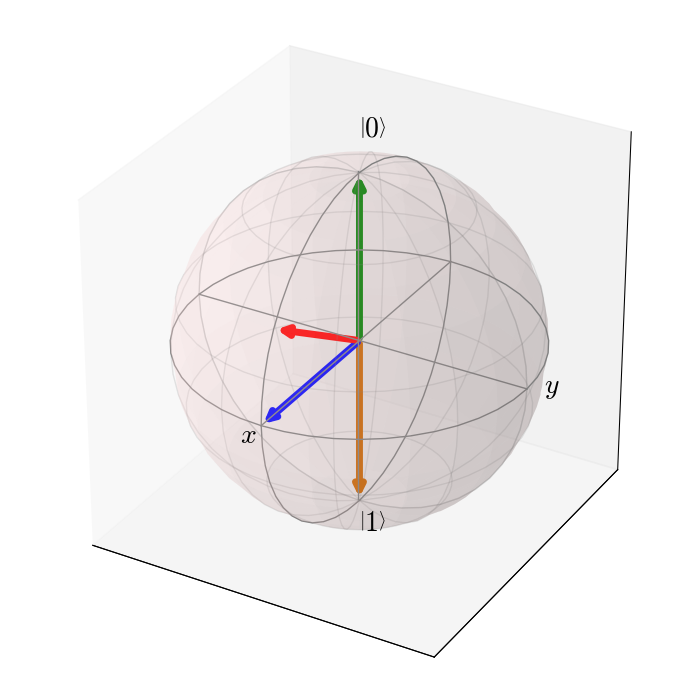
\includegraphics[height=7cm]{graphics/Bloch3.png}
\caption{Représentation avec QuTiP de la sphère de Bloch avec les états 
$\ket{0}$, $\ket{1}$ et $(\ket{0}+\ket{1})/\sqrt{2}$.}
\end{center}
\end{figure}

\begin{exercise}
For each of the following qubits, if a measurement is made, what is the
probability that we find the qubit in the state $\ket{0}$? What is the
probability that we find the qubit in the state $\ket{1}$?
\begin{enumerate}
 \item $\ket{\psi}=\frac{1}{\sqrt{3}}\ket{0}+\sqrt{\frac{2}{3}}\ket{1}$.
 \item $\ket{\psi}=\frac{i}{2}\ket{0}+\frac{\sqrt{3}}{2}\ket{1}$.
 \item $\ket{\psi}=\frac{1+i}{\sqrt{3}}\ket{0}-\frac{i}{\sqrt{3}}\ket{1}$.
\end{enumerate}
 Compute with QuTiP the probabilities of finding the state $\ket{\psi}$ in 
$\ket{0}$ or in $\ket{1}$. Plot on the Bloch sphere the state $\ket{0}$, 
$\ket{1}$ and $\ket{\psi}$.
\end{exercise}

\begin{footnotesize}
\begin{solution}
 To find the probability that each qubit is found in the state $\ket{0}$ or the
state $\ket{1}$, we compute the modulus squared of the appropriate coefficient.
\begin{enumerate}
 \item The probability of finding $\ket{\psi}$ in the state $\ket{0}$ is
\begin{subequations}
\begin{align}
\left|\frac{1}{\sqrt{3}}\right|^{2}=\frac{1}{3},
\end{align}
whereas probability of finding $\ket{\psi}$ in the state $\ket{1}$ is
\begin{align}
 \left|\sqrt{\frac{2}{3}}\right|^{2}=\frac{2}{3}.
\end{align}
These probabilities verified
\begin{align}
 \sum_{i=0}^{1}|\alpha_{i}|^{2}=\frac{1}{3}+\frac{2}{3}=1.
\end{align}
\end{subequations}
  \item The next state has coefficients that are complex numbers. So that
the probability of finding $\ket{\psi}$ in the state $\ket{0}$ is
\begin{subequations}
\begin{align}
\left|\frac{i}{2}\right|^{2}=\left(\frac{i}{2}\right)^{*}\left(\frac{i}{2}
\right)=\left(-\frac{i}{2}\right)\left(\frac{i}{2}\right)=\frac{1}{4},
\end{align}
whereas probability of finding $\ket{\psi}$ in the state $\ket{1}$ is
\begin{align}
 \left|\frac{\sqrt{3}}{2}\right|^{2}=\frac{3}{4}.
\end{align}
Again, we check that the probabilities sum to $1$:
\begin{align}
 \sum_{i=0}^{1}|\alpha_{i}|^{2}=\frac{1}{4}+\frac{3}{4}=1.
\end{align}
\end{subequations}
  \item Finally, for the last state, the probability of finding $\ket{\psi}$ in
the state $\ket{0}$ is
\begin{subequations}
\begin{align}
\left|\frac{1+i}{\sqrt{3}}\right|^{2}=\left(\frac{1+i}{\sqrt{3}}
\right)^{*}\left(\frac{1+i}{\sqrt{3}}\right)=\left(\frac{1-i}{\sqrt{3}}
\right)\left(\frac{1+i}{\sqrt{3}}\right)=\frac{1-i+i+1}{3}=\frac{2}{3},
\end{align}
whereas probability of finding $\ket{\psi}$ in the state $\ket{1}$ is
\begin{align}
 \left|\frac{i}{\sqrt{3}}\right|^{2}=\left(\frac{i}{\sqrt{3}}
\right)^{*}\left(\frac{ i}{\sqrt{3}}\right)=\left(-\frac{i}{\sqrt{3}}
\right)\left(\frac{ i}{\sqrt{3}}\right)=\frac{1}{3} .
\end{align}
Again, these probabilities sum to $1$:
\begin{align}
 \sum_{i=0}^{1}|\alpha_{i}|^{2}=\frac{2}{3}+\frac{1}{3}=1.
\end{align}
\end{subequations}

\end{enumerate}
As the probability of finding the state $\ket{\psi}$ in $\ket{i}$ is given by 
$p_i=|\bra{i}\psi\rangle|^2=\bra{i}\psi\rangle\bra{i}\psi\rangle^*$, $i=0,1$, 
the QuTiP script should be \\
\begin{tt}
from qutip import *\\
ket0 = basis(2,0)\\
bra0 = ket0.dag()\\
ket1 = basis(2,1)\\
bra1 = ket1.dag()\\
psi = (ket0+sqrt(2)*ket1)/sqrt(3) \\
p0 = (bra0*psi)*(bra0*psi).dag()\\
p1 = (bra1*psi)*(bra1*psi).dag()
\end{tt}
Do the same for the other cases.

\textbf{\emph{Pas du tout compliqué n'est-ce pas?}}
\end{solution}
\end{footnotesize}

\subsection{Espace de Hilbert}
\label{sec:EH}

L'espace mathématique où ont lieu les calculs quantiques est l'\textbf{espace de
Hilbert} $\mathcal{H}$, qui est un espace Euclidien complexe, muni d'un produit
scalaire. C'est un espace de dimension infinie, mais nous nous limiterons dans
cette section au cas de la dimension finie.
\begin{enumerate}
\item Le \textbf{ket} $\ket{i}$ est un vecteur de l'espace des états ou
\textbf{espace de Hilbert }$\mathcal{H}$;

\item Le \textbf{bra} $\bra{f}$ est un vecteur de l'espace dual
$\mathcal{H}^{\ast}$, autrement, c'est le \textbf{conjugué hermitien} du
$\ket{f}$,
\begin{equation}
 (\ket{f})^{\dag}=\bra{f}.
\end{equation}
\end{enumerate}

Il existe une correspondance biunivoque entre les vecteurs de ces deux
espaces. On utilise le même symbole pour représenter un vecteur de l'un de ces
espaces et celui qui lui correspond dans l'autre espace. Ainsi, le vecteur de
l'espace des états correspondant au bra $\bra{f}$ est le ket $\ket{f}$.

\subsubsection{Base hilbertienne}

\medskip\colorbox[gray]{0.8}{
\parbox[c]{0.9\textwidth}{
\begin{definition}
L'ensemble $\mathcal{B}=\{\ket{i}\}$ est \textbf{une base hilbertienne}, si
\begin{equation}
\langle i\ket{j} =\delta_{ij}=\begin{cases}
1 & \text{si }i=j,\\
0 & \text{sinon,}
\end{cases}
\label{eq:dij}
\end{equation}
et
\begin{equation}
\sum_{i\in\mathcal{B}}\ket{i}\bra{i}=\mathbf{1}.
\label{eq:RF}
\end{equation}
La \textbf{relation de fermeture} (\ref{eq:RF}) permet la projection d'un
vecteur d'état dans la base $\mathcal{B}$.
\end{definition}
}}

Ainsi, le ket $\ket{y} $ se développe dans la base hilbertienne $\mathcal{B}$,
compte tenu de la relation de fermeture (\ref{eq:RF}), sous la forme%
\begin{subequations}
\begin{align}
\ket{y} =\sum_{i\in B}\ket{i} \langle i\ket{y} =\alpha_{i}\ket{i},
\end{align}
\label{eq:XY}%
avec%
\begin{align}
\alpha_{i}=\langle i\ket{y},
\end{align}
\end{subequations}
considérée ici comme la \textbf{coordonnée} ou la \textbf{projection} ou plus
précisément \textbf{l'amplitude de probabilité de projection} de $\ket{y}$
suivant $\ket{i}$.

Puisque le bra $\bra{x}$ appartient à \textbf{l'espace dual}
$\mathcal{H}^{\ast}$, on a la correspondance antilinéaire \textbf{ket}
$\rightarrow$\textbf{bra}:
\begin{subequations}%
\begin{align}
\lambda\ket{\psi}  &  \longrightarrow\lambda^{\ast}\bra{\psi},\\
\lambda_1\ket{\psi_1}+\lambda_2\ket{\psi_2}&
\longrightarrow\lambda_1^{\ast}\bra{\psi}_1+\lambda_2^{\ast}
\bra{\psi_2}.
\end{align}%
\end{subequations}%
Par suite,
\begin{equation}
\bra{x} =\sum_{i\in B}\langle x\ket{i}\bra{i} =\sum_{i\in B}\langle i\ket{x}
^{\ast}\bra{i} =\alpha_{i}^{\ast}\bra{i}.
\end{equation}
C'est ainsi que, dans base $\{\ket{i}\}$, les vecteurs d'états sont représentés
dans $\mathcal{H}$ par des nombres, valeurs des composantes ou amplitudes de
transition ou de projection:
\begin{subequations}%
\begin{align}
\ket{\psi} &  =\sum_{i}\ket{i}\langle i\ket{\psi}=\sum_{i}\alpha_{i}\ket{i}
\text{ avec }\langle i\ket{\psi} =\alpha_{i}\Rightarrow\ket{\psi} =
\begin{pmatrix}
\alpha_1\\
\alpha_2\\
\vdots\\
\alpha_{i}\\
\vdots
\end{pmatrix},\\
\bra{\psi} &  =\sum_{i}\langle\psi\ket{i}\bra{i}=\sum_{i}\bra{i}
\alpha_{i}^{\ast}\text{ avec }\bra{\psi}i\rangle=\alpha_{i}^{\ast}
\Rightarrow\bra{\psi}=(\alpha_1^{\ast},\alpha_2^{\ast},\cdots,\alpha_{i}^{
\ast},\cdots).
\end{align}%
\end{subequations}%

Si un vecteur $\ket{\varphi}$ se décompose sur la base $\{\ket{i}\}$ suivant
\begin{equation}
\ket{\varphi} =\sum_{i}\beta_{i}\ket{i},
\end{equation}
alors, en utilisant (\ref{eq:dij})%
\begin{equation}
\langle\psi\ket{\varphi} =\sum_{i,j=1}\langle\psi\ket{i}\bra{i}
j\rangle\langle j\ket{\varphi}=\sum_{i}\alpha_{i}^{\ast}\beta_{i}.
\label{eq:XY2}
\end{equation}

La notion d'état de la base hilbertienne peut être très bien comprise à
travers l'analogie avec l'espace $\mathcal{V}$ des vecteurs réels
tridimensionnels.

Considérons les vecteurs de base de $\mathcal{V}$%
\begin{equation}
\bls{e}_1=\begin{pmatrix}
1\\
0\\
0
\end{pmatrix},\ \bls{e}_2=\begin{pmatrix}
0\\
1\\
0
\end{pmatrix},\ \bls{e}_{3}=\begin{pmatrix}
0\\
0\\
1
\end{pmatrix},
\end{equation}
et deux vecteurs de $\mathcal{V}$%
\begin{equation}
\bls{A}=\begin{pmatrix}
a_1\\
a_2\\
a_{3}\end{pmatrix},\ \bls{B}=\begin{pmatrix}
b_1\\
b_2\\
b_{3}\end{pmatrix}.
\end{equation}
Le vecteur
\begin{equation}
\bls{B}=\sum_{i=1}^{3}\bls{e}_{i}(\bls{e}_{i}
\cdot\bls{B})=\sum_{i=1}^{3}\bls{e}_{i}b_{i}=
b_1\bls{e}_1+b_2\bls{e}_2+b_{3}\bls{e}_{3}.
\label{eq:B}%
\end{equation}
qui apparaît comme la somme de ces composantes ou projections sur les vecteurs
de base, est l'analogue de la relation (\ref{eq:XY}).

L'analogue de la relation (\ref{eq:XY2}) est
\begin{equation}%
\begin{split}
\bls{A}\cdot\bls{B}  &  =\sum_{i=1}^{3}(\bls{A}\cdot\bls{e}_{i})
(\bls{e}_{i}\cdot\bls{B})\\
& =(\bls{A}\cdot\bls{e}_1)(\bls{e}_1\cdot\bls{B})
+(\bls{A}\cdot\bls{e}_2)(\bls{e}_2\cdot\bls{B})
+(\bls{A}\cdot\bls{e}_{3})(\bls{e}_{3}\cdot\bls{B})
\\
&  =a_1b_1+a_2b_2+a_{3}b_{3}.
\label{eq:AB2}%
\end{split}%
\end{equation}%
On note que les vecteurs $\bls{A}$ et $\bls{B}$ correspondent aux deux vecteurs
états $\ket{\psi} $ et $\ket{\varphi} $ et l'ensemble des vecteurs de base
correspondent à l'ensemble des vecteurs d'états de la base hilbertienne.

\begin{example}
Dans la base $\{\ket{+},\ket{-}\}$, l'état superposé $\ket{\psi}
=\frac{1}{\sqrt{2}}(\ket{+}+\ket{-})$ a pour composantes
\begin{equation}
\ket{\psi} =\frac{1}{\sqrt{2}}\left(\begin{pmatrix}
1\\
0
\end{pmatrix}+\begin{pmatrix}
0\\
1
\end{pmatrix}\right)=\frac{1}{\sqrt{2}}\begin{pmatrix}
1\\
1
\end{pmatrix}.
\end{equation}
\end{example}

\begin{example}
Soit un système quantique décrit dans la base d'états $\{\ket{a},\ket{b},\ket{c}
\}$. Dans cette représentation, les états $\ket{\psi} $ et $\ket{\varphi}$ ont
les amplitudes
\begin{subequations}%
\begin{align}
\langle a\ket{\psi}  &  =\frac{1}{\sqrt{3}},~\langle b\ket{\psi} =0,~\langle
c\ket{\psi}=i\sqrt{\frac{2}{3}},\\
\langle a\ket{\varphi} &  =\frac{1+i}{\sqrt{3}},~\langle b\ket{\varphi}
=\frac{1}{\sqrt{6}},~\langle c\ket{\varphi}=\frac{1}{\sqrt{6}}.
\end{align}
\end{subequations}%
La probabilité de trouver le système dans l'état $\ket{\varphi}$ alors qu'il se
trouvait initialement dans l'état $\ket{\psi}$ est
\begin{equation}%
\mathcal{P}_{\varphi\psi} =|\langle\varphi\ket{\psi}|^{2}=\left|
\sum_{i}\langle\varphi\ket{i}\langle i\ket{\psi}\right|^{2}=\left|
\frac{1\times(1-i)}{3}+0+i\sqrt{\frac{2}{3\times6}}\right|^{2}=\left|
\frac{1}{3}\right|^{2}=\frac{1}{9}.
\end{equation}%
Il est facile de vérifier que $\mathcal{P}_{\psi\varphi} =|\frac{1}{3}|^{2}
=\frac{1}{9}$.
\end{example}

\begin{exercise}
 Two vectors in $\mathbb{C}^{3}$ are given by $\ket{a}=\begin{pmatrix}
-2\\
4i\\
1
\end{pmatrix}$ and $\ket{b}=\begin{pmatrix}
1\\
0\\
i
\end{pmatrix}$.

Find
\begin{enumerate}
 \item $\bra{a}$, $\bra{b}$.
 \item $\langle a\ket{b}$, $\langle b\ket{a}$.
 \item $\ket{c}=\ket{a}+2\ket{b}$, $\langle c\ket{a}$.
\end{enumerate}
\end{exercise}

\begin{footnotesize}
\begin{solution}
 \begin{enumerate}
  \item The Hermitian conjugate is the complex conjugate of the transpose. Then,
\begin{subequations}
\begin{align}
 \bra{a}=(\ket{a})^{\dag}=(\ket{a}^{t})^{*}=(-2\quad-4i\quad 1),\\
 \bra{b}=(\ket{b})^{\dag}=(\ket{b}^{t})^{*}=(1\quad0\quad-i).
\end{align}
\end{subequations}
  \item From (\ref{eq:XY2}), the probability amplitude
\begin{subequations}
\begin{align}
 \langle a\ket{b}=(-2\quad-4i\quad 1)\begin{pmatrix}
1\\
0\\
i
\end{pmatrix}=-2+0+i=-2+i.
\end{align}
As $\langle a\ket{b}=\langle b\ket{a}^{*}$, we should find $\langle
b\ket{a}=-2-i$. We verify this with an explicit calculation
\begin{align}
 \langle b\ket{a}=(1\quad0\quad-i)\begin{pmatrix}
-2\\
4i\\
1
\end{pmatrix}=-2+0-i=-2-i.
\end{align}
\end{subequations}
 \item We apply the rules of vector addition and scalar multiplication to
obtain
\begin{subequations}
\begin{align}
 \ket{c}=\ket{a}+2\ket{b}=\begin{pmatrix}
-2\\
4i\\
1
\end{pmatrix}+2\begin{pmatrix}
1\\
0\\
i
\end{pmatrix}=\begin{pmatrix}
-2+21\\
4i+0\\
1+2i
\end{pmatrix}=\begin{pmatrix}
0\\
4i\\
1+2i
\end{pmatrix}
\end{align}
Therefore
\begin{align}
 (0\quad-4i\quad1-2i)\begin{pmatrix}
-2\\
4i\\
1
\end{pmatrix}=0+16+1-2i=17-2i.
\end{align}

\end{subequations}
 \end{enumerate}
\textbf{\emph{Aussi simple que ce qu'on apprend au Secondaire n'est-ce pas?}}
\end{solution}
\end{footnotesize}

\subsubsection{Produit scalaire}

Si on a
\begin{equation}
 \langle x\ket{y}=0,
\end{equation}
alors $\ket{x}$ et $\ket{y}$ sont \textbf{orthogonaux}. La symétrie hermitienne
du produit scalaire
\begin{equation}
 \langle x\ket{y}^{*}=\langle y\ket{x},
\end{equation}
implique que $\langle y\ket{y} $ est \emph{un nombre réel défini positif}%
\begin{subequations}
\begin{align}
\langle y\ket{y} \leq 0,
\end{align}
et
\begin{align}
\langle y\ket{y} =0\Rightarrow\ket{y} =0.
\end{align}
\end{subequations}

La \textbf{norme} d'un vecteur d'état $\ket{y} $ est définie par%
\begin{equation}
\|\ket{y}\| =\sqrt{\langle y\ket{y}}.
\end{equation}

Lorsque
\begin{equation}
 \langle x\ket{x}=1,
\end{equation}
on dit que le vecteur d'état $\ket{x}$ est \textbf{normalisé}.

Si chaque élément d'une base est normalisé et que les éléments de la base sont
orthogonaux les uns par rapport aux autres, on dit que la base est
\textbf{orthonormée}. C'est par exemple le cas de la base $\{\ket{+},\ket{-}\}$
avec
\begin{equation}
 \ket{+}=\frac{1}{\sqrt{2}}\binom{1}{1} ,\;
 \ket{+}=\frac{1}{\sqrt{2}}\binom{1}{-1}.
\end{equation} '
Une des propriétés importantes du produit scalaire est l'\emph{inégalité de
Cauchy-Schwarz}%
\begin{equation}
|\langle x\ket{y}|^{2}\leq\langle x\ket{x}\langle y\ket{y}
=\|\ket{x}\|^{2}\|\ket{y}\|^{2}.
\end{equation}

Maintenant que nous sommes un tout peu outillé en manipulations
mathématiques du qubit, des amplitudes de probabilités, des
probabilités, essayons de mieux les comprendre physiquement.

\section{Phénomènes quantiques: Interférence à une particule}

\label{sec:Inter1Part}

Afin de mettre en évidence l'étrange comportement des qubits, quelques
expériences ont été réalisées avec des objets quantiques (photons, électrons,
neutrons, atomes, molécules) isolées, ce qui écarte l'hypothèse des effets
collectifs\footnote{Mécanisme au terme duquel le sort d'un objet quantique
conditionnerait celui du suivant.}.
\bigskip

\emph{Rendons-nous donc au laboratoire!!}

\subsection{Fentes d'Young}

Commençons par le dispositif des fentes d'Young de la figure \ref{fig:DispYoung}
qui nous est très familier. La source $S$ émet un faisceau lumineux et le
détecteur mesure l'intensité lumineuse pour différentes positions de $x$. Si une
seule fente est ouverte, l'intensité est maximale à la position $x$ alignée
horizontalement sur la fente $F_1$. Lorsqu'on éloigne le détecteur de cette
position $x$, l'intensité diminue progressivement et devient nulle. Cependant,
lorsque les deux fentes sont ouvertes, la figure des intensités n'est pas
\textit{la somme} des deux figures d'intensité des fentes individuelles
ouvertes, mais plutôt une figure d'interférence: \textit{on observe au détecteur
une alternance de franges brillantes et de franges sombres} (voir la figure
\ref{fig:InterfLum}). Il y a donc interférence entre les faisceaux lumineux
provenant des deux fentes.

\begin{figure}[tbhp]
\begin{minipage}[c]{.48\linewidth}
\centering
\ifcase\msipdfoutput
	\includegraphics[scale=1]{graphics/DispYoung.eps}%
\else
	\includegraphics[scale=1]{graphics/DispYoung.pdf}%
\fi
\caption{Dispositif des fentes de Young}
\label{fig:DispYoung}%
\end{minipage} \hfill\begin{minipage}[c]{.48\linewidth}
\centering
\ifcase\msipdfoutput
	\includegraphics[scale=1]{graphics/InterfLum.eps}%
\else
	\includegraphics[scale=1]{graphics/InterfLum.jpg}%
\fi
\caption{Interférence lumineuse lorsque les deux fentes sont ouvertes. On a
une alternance de franges brillantes et de franges sombres.}%
\label{fig:InterfLum}%
\end{minipage}
\end{figure}

Utilisons maintenant un dispositif spécial dont la source $S$ ne produit que des
électrons uniques qui sont dirigés vers les fentes $F_1$ et $F_2$.
L'électron a une charge bien déterminée et la proposition \emph{un seul électron
est bien passé soit par $F_1$, soit par $F_2$} est bien décidable (deux
\textbf{chemins possibles}). Chaque électron est capté en un \emph{point bien
précis} du détecteur comme on peut le voir sur la figure \ref{fig:InterfPhotons}
(a). Ces points d'impact sont cependant \textbf{aléatoires}: les différents
électrons indépendants préparés dans les \emph{mêmes} conditions ont des impacts
\emph{différents}. Ce qui est en contradiction avec le
\textbf{\emph{déterminisme}} classique qui veut à des \emph{conditions initiales
identiques}, correspondent des \emph{conditions finales identiques}.

\begin{figure}[htbp]
\centering
\ifcase\msipdfoutput
  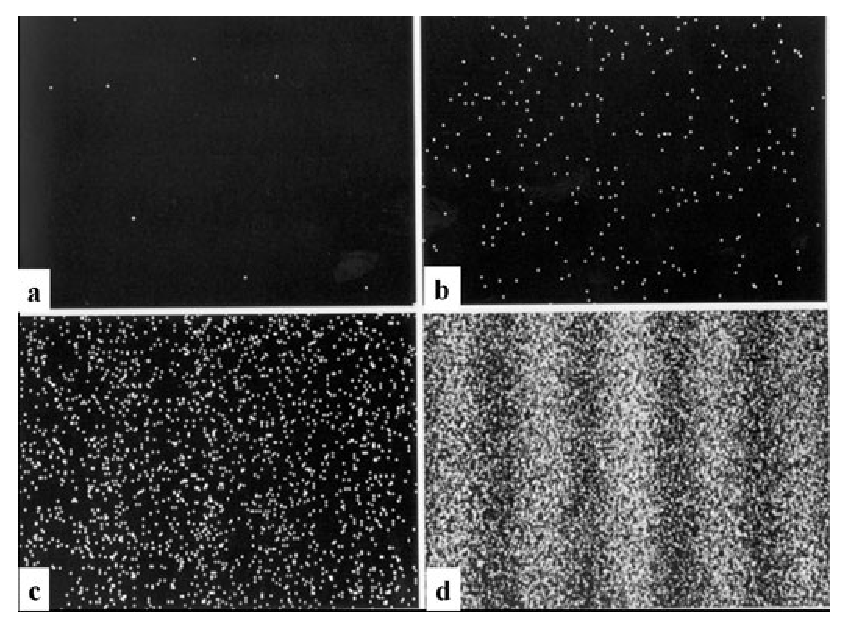
\includegraphics[scale=1]{graphics/InterfPhotons.eps}%
\else
  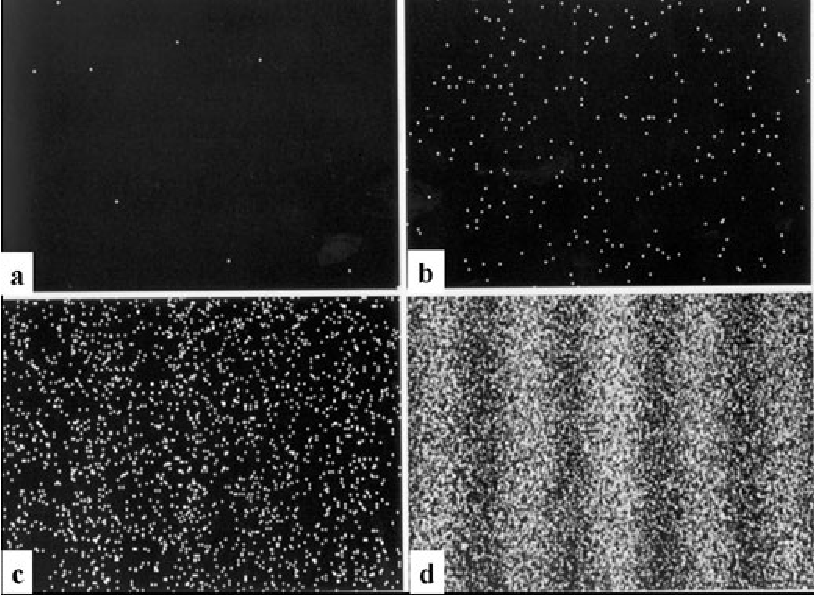
\includegraphics[scale=1]{graphics/InterfPhotons.pdf}%
\fi
\caption{Figures d'interférence obtenues avec des électrons uniques. Le nombre
d'électrons sur le détecteur augmente au cours du temps. Le temps d'exposition
entre la figure (a) et la figure (d) est multiplié par $20$. (a) 8 électrons;
(b) 270 électrons; (c) 2000 électrons; (d) 6000 électrons. [D'après Hitachi
Advanced Research Laboratory, Saitama, Japan].}%
\label{fig:InterfPhotons}%
\end{figure}

Au bout \emph{d'un temps suffisamment long}, on observe avec surprise que les
impacts des électrons forment une figure d'interférence comme illustrée par la
figure \ref{fig:InterfPhotons} (d). Ce résultat est surprenant en ce sens que
l'électron est un \textbf{corpuscule}. Or nous savons q'une onde emplit tout
l'espace! Les électrons sont uns et \textbf{indivisibles}, donc il n'y a pas de
fragmentation d'un quantum d'énergie $\hbar\omega$. D'après Paul Dirac,
\textbf{chaque électron interfère avec lui-même} comme une onde\footnote{En
fait, avant la mesure, l'électron est dans une \textbf{superposition d'états},
et c'est chacun de ces états qui a interféré avec les autres.}. Il y a donc
antinomie: \emph{les concepts classiques d'onde et de corpuscules semblent ne
plus être valables pour les objets quantiques.}

Lorsqu'on réalise une autre expérience où le chemin emprunté par l'électron est
\textbf{discernable}, $F_1$ ouvert seul ou $F_2$ ouvert seul, on n'observe
pas de figure d'interférence, mais plutôt des impacts distribués autour des
sorties $F_1$ ou $F_2$. La somme de ces deux distributions distinctes ne
ressemble en rien la figure obtenue quand les deux fentes sont ouvertes. On ne
peut donc analyser le phénomène d'interférence des électrons uniques en termes
de probabilité classique: \textbf{\emph{lorsqu'à la même issue correspondent des
processus indépendants différents, la probabilité de cette issue n'est pas la
somme des probabilités individuelles}}.

\subsection{Interférométrie de Mach Zehnder}
\label{sec:InterfMZ}

Afin de mieux analyser le comportement des objets quantiques, examinons, après
V. Scarani\cite{VSC2004}, les expériences qui mènent à l'interférométrie de Mach
Zehnder. On a (voir les figures \ref{fig:MZ1}-\ref{fig:MZ4}):
\begin{itemize}
\item une \emph{source} qui envoie des objets quantiques isolés, un à un, l'un
après l'autre;

\item des \emph{séparateurs} qui sont des miroirs semi-transparents;

 \item et des \emph{détecteurs}, dispositifs de mesure permettant de compter les
objets quantiques.
\end{itemize}

\begin{figure}[ptbh]
\begin{minipage}[c]{.48\linewidth}
\centering
\ifcase\msipdfoutput
	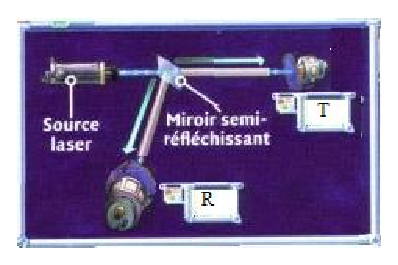
\includegraphics[scale=1]{graphics/MZ1.eps}%
\else
	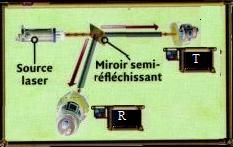
\includegraphics[scale=1]{graphics/MZ1.jpg}%
\fi
\caption{\emph{\textbf{Expérience MZ1:}} Montage à $2$ chemins ou fonctionnement
d'un miroir semi-transparent.}
\label{fig:MZ1}%
\end{minipage} \hfill\begin{minipage}[c]{.48\linewidth}
\centering
\ifcase\msipdfoutput
	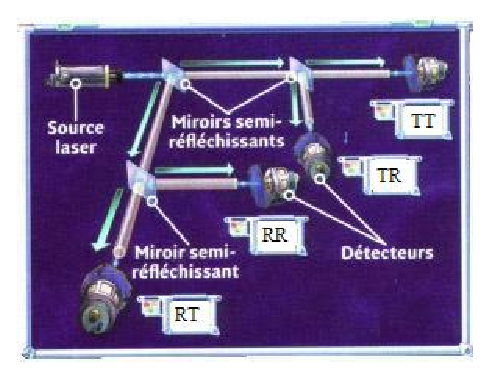
\includegraphics[scale=.9]{graphics/MZ2.eps}%
\else
	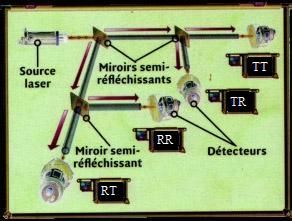
\includegraphics[scale=.9]{graphics/MZ2.jpg}%
\fi
\caption{\emph{\textbf{Expérience MZ2:}} Montage à
$4$ chemins avec $3$ miroir semi-transparents.}%
\label{fig:MZ2}%
\end{minipage}
\end{figure}

\subsection{Expérience MZ1}

Figure \ref{fig:MZ1}: Les objets quantiques arrivent individuellement sur le
séparateur et on compte combien d'entre eux sont réfléchis (R), et combien sont
transmis (T). Après le passage d'un grand nombre d'objets quantiques, on fait
les deux observations suivantes:

\begin{enumerate}
\item Les deux détecteurs ne s'activent jamais au même instant, donc
l'objet est \textbf{indivisible}, \emph{il est soit réfléchi, soit transmis}
(deux \textbf{chemins} possibles);

\item On dénombre la moitié des objets en R et l'autre en T, donc \emph{la
probabilité pour qu'un objet quantique soit réfléchi est la même qu'il soit
transmis} et les deux probabilités sont $50\%$.
\end{enumerate}

\subsection{Expérience MZ2}

Il y a lieu de se poser la question de savoir si en sortant de la source,
chaque objet n'a pas une \emph{instruction} lui permettant, chaque fois qu'il
rencontre un séparateur, d'être soit seulement réfléchie, soit seulement
transmis?

Afin d'élucider cela, à chaque sortie du premier séparateur, on place un autre
séparateur et on obtient \emph{quatre} chemins possibles (figure \ref{fig:MZ2}
): l'objet quantique peut être réfléchi deux fois (RR), réfléchi puis transmis
(RT), transmis puis réfléchi (TR) ou transmis deux fois (TT).

Si chaque objet avait une \emph{instruction} lui permettant, chaque fois qu'il
rencontre un séparateur, d'être soit seulement réfléchie, soit seulement
transmis, alors après le passage d'un grand nombre d'objets quantiques,
on observerait $50\%$ des objets en RR et $50\%$ des objets en TT, et rien en
RT\ ou TR.

Mais on observe qu'à chaque sortie, on a $25\%$ d'objets à chaque sortie.

\subsection{Expérience MZ3}

Figure \ref{fig:MZ3}: On a maintenant un interféromètre de Mach Zehnder: à
chaque sortie du premier séparateur, on place maintenant un miroir parfait qui
réfléchi tous les objets, les orientant vers un deuxième séparateur. Ainsi, une
des sorties du deuxième séparateur correspond aux chemins RT ou TR, l'autre aux
chemins RR ou TT. On a donc a nouveau quatre chemins possibles, de longueur
égale.

En vertu de la deuxième expérience, à la sortie RT ou TR, on observera
$25\%+25\%=50\%$ d'objets quantiques, et à la sortie RR ou TT, $50\%$ d'objets
quantiques.

Cependant, on observe que \emph{\textbf{tous les objets quantiques se trouvent
à la sortie RT ou TR}}: \textbf{le chemin RT est indiscernable du chemin TR}
après détection. \emph{On ne peut savoir quel chemin l'objet quantique détecté a
pris!}

On dit qu'il y a une \emph{\textbf{interférence constructive}} à la sortie RT
ou TR et une \emph{\textbf{interférence destructive}} à la sortie TT ou RR.
Puisqu'il y a une seule particule à la fois, on parle \textbf{d'interférence à
une particule}. Concrètement, un pic d'intensité sur une des sorties
correspond à un creux à l'autre sortie et inversement.

\medskip
\colorbox[gray]{0.8}{
\parbox[c]{0.9\textwidth}{
\emph{Le hasard quantique est vraiment étrange: lorsqu'on assemble d'une
certaine manière deux diviseurs de faisceau ou beam-splitters (générateurs de
hasard), on retrouve la certitude!}
}}
\medskip

Posons-nous les deux questions suivantes qui admettent les réponses \emph{oui}
ou \emph{non}:

\begin{enumerate}
\item[\textbf{Q1:}] l'objet quantique a-t-il pris le chemin T après le premier
séparateur?

\item[\textbf{Q2:}] l'objet quantique est-il détecté à la sortie RT ou TR?
\end{enumerate}

Dans la configuration de notre expérience MZ3, Q2 est toujours \emph{oui},
mais ne pouvons pas répondre à Q1.

Si on modifie l'expérience en insérant des détecteurs aux chemins R et T après
le premier séparateur, de sorte à pouvoir répondre à Q1, alors la réponse à la
question Q2 est modifiée. Seule la moitié des objets quantiques donneront la
réponse \emph{oui}, conformément à l'expérience MZ1. Donc si l'objet quantique
laisse une \emph{trace} de son passage, on observe pas d'interférence.

\medskip
\colorbox[gray]{0.8}{
\parbox[c]{0.9\textwidth}{
\emph{Il est donc impossible de savoir par quel chemin est passé l'objet
quantique et observer les interférences.} C'est le paradoxe connu sous le nom
du \emph{\textbf{chat de Schrödinger}}.
}}

\begin{figure}[ptbh]
\begin{minipage}[c]{.48\linewidth}
\centering
\ifcase\msipdfoutput
	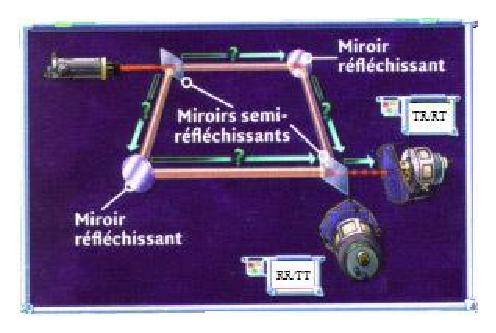
\includegraphics[scale=1]{graphics/MZ3.eps}%
\else
	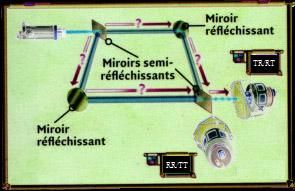
\includegraphics[scale=1]{graphics/MZ3.jpg}%
\fi
\caption{\emph{\textbf{Expérience MZ3:}} Interféromètre de Mach Zehnder
équilibré. \emph{\textbf{Les
chemins sont indiscernables.}}}
\label{fig:MZ3}%
\end{minipage} \hfill\begin{minipage}[c]{.48\linewidth}
\centering
\ifcase\msipdfoutput
	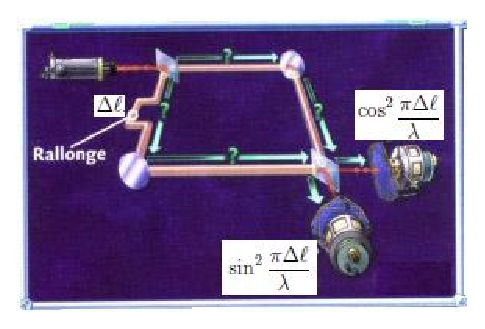
\includegraphics[scale=1]{graphics/MZ4.eps}%
\else
	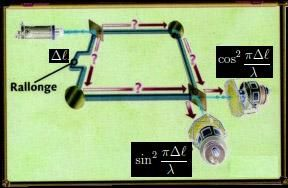
\includegraphics[scale=1]{graphics/MZ4.jpg}%
\fi
\caption{\emph{\textbf{Expérience MZ4:}} Interféromètre de Mach Zehnder
déséquilibré.
\emph{\textbf{Les chemins sont discernables et l'objet quantique explore tous
les chemins
possibles.}}}%
\label{fig:MZ4}%
\end{minipage}
\end{figure}

\subsection{Expérience MZ4}

Figure \ref{fig:MZ4}: On modifie la longueur des chemins RT ou TR, en y
introduisant par exemple une longueur supplémentaire $\Delta\ell$. On constate
que les probabilités de détection des objets quantiques aux sorties (RT ou TR)
et (RR ou TT) sont respectivement%
\begin{equation}
\cos^{2}\frac{\varphi}{2}\text{ et }\sin^{2}\frac{\varphi}{2},\ \varphi
=2\pi\frac{\Delta\ell}{\lambda}.
\end{equation}
Ainsi, lorsque par exemple,

\begin{itemize}
\item $\Delta\ell=\lambda$ (lame d'onde), tous les objets quantiques sont
détectés à la
sortie RT ou TR.

\item $\Delta\ell=\frac{\lambda}{2}$ (lame demi-d'onde), tous les objets
quantiques sont détectés
à la sortie RR ou TT;

\item $\Delta\ell=\frac{\lambda}{4}$ (lame quart-d'onde), une moitié des objets
quantiques est détectés à la
sortie RR ou TT et l'autre moitié à la sortie RT ou TR;

\end{itemize}

\medskip
\colorbox[gray]{0.8}{
\parbox[c]{0.9\textwidth}{
\emph{Donc, lorsqu'on modifie un seul des deux chemins, on modifie le
comportement des tous les objets quantiques.}
}}
\medskip

Comme on peut le voir sur les figures d'interférences \ref{fig:FiguresInterMZ},
les différences de longueurs d'onde pour lesquelles toute la lumière est
détectée dans RT ou TR correspondent à des pics d'intensité maximale (franges
brillantes, interférences constructives) dans le montage des fentes d'Young.
Les différences de longueurs d'onde pour lesquelles toute la lumière est
détectée dans RR ou TT correspondent à des creux d'intensité nulle (franges
sombres, interférences destructives) dans le montage des fentes d'Young.

\begin{figure}[ptbh]
\centering
\ifcase\msipdfoutput
  \includegraphics{graphics/FiguresInterfMZ.png}
\else
  \includegraphics{graphics/FiguresInterfMZ.pdf}
\fi
\caption{Figures d'interférences obtenues au détecteur RT ou TR et RR ou TT.
La complémentarité des franges est remarquable.}%
\label{fig:FiguresInterMZ}%
\end{figure}

\subsubsection{En résumé}

\begin{enumerate}
\item Chaque objet quantique est indivisible lors de la détection, comme un
\textbf{corpuscule}.

\item Dans les expériences MZ1 et MZ2, il y a un seul chemin qui conduit à
chaque
détecteur; chaque objet quantique détecté a emprunté un chemin connu:
\emph{c'est la situation de \textbf{discernabilité}, il n'y a pas
d'interférence.}

\item Dans les expériences MZ3 et MZ4, on ne peut dire quel chemin chaque objet
quantique détecté a emprunté, puisque que deux chemins sont possibles.
\emph{Ces deux chemins sont indiscernables et les effets d'interférence sont
présents.} On peut donc énoncer le principe suivant:

\colorbox[gray]{0.8}{
\parbox[c]{0.9\textwidth}{
\begin{principe}[Indiscernabilité des chemins] Les interférences apparaissent
lorsqu'un objet quantique peut emprunter plusieurs chemins pour arriver au même
détecteur, et que ces chemins sont \textbf{indiscernables} après la détection.
\end{principe}
}}

On peut dire que le comportement des objets quantiques dépend de toutes les
possibilités indiscernables.

\item Chaque objet quantique explore tous les chemins possibles
(\emph{\textbf{délocalisation}}) comme une onde, cependant elle est
indivisible à la détection. Si cette exploration de tous les chemins n'était
pas possible, toutes les objets quantiques ne seraient pas influencés par le
changement de longueur d'un seul chemin.

\medskip\colorbox[gray]{0.8}{
\parbox[c]{0.9\textwidth}{
\emph{Un objet quantique n'a donc pas \textbf{une trajectoire} bien définie.}
}}

\item Dans l'expérience MZ3, lorsqu'on cherche à savoir par quel chemin est
passé l'objet quantique, on n'observe plus de figure d'interférence. On dit
alors que

\medskip\colorbox[gray]{0.8}{
\parbox[c]{0.9\textwidth}{
\emph{ \textbf{la mesure perturbe le système}: il y a une perturbation
incontrôlable de l'objet quantique par la mesure}. La description quantique des
phénomènes doit englober l'effet de l'appareil de mesure.
}}\medskip

L'interposition d'un instrument de mesure modifie le chemin emprunté et la
discernabilité apparaît.

Ce phénomène est d'ailleurs à la base de la \emph{cryptographie
quantique}\footnote{Le sécurité de la communication de la Coupe du Monde 2010 à
été confiée à société de cryptographie quantique \emph{ID Quantique} fondée par
Nicolas Gisin de l'Université de Genève.} car toute tentative d'espionnage est
immédiatement détectée par la perturbation qu'elle introduit.
\end{enumerate}

Soulignons que depuis les années '70, on a pu observer des figures
d'interférences avec des objets quantiques aussi divers que photons, les
neutrons, les atomes et même de molécules comme les fullèrenes ou
footballènes\footnote{[Zeilinger \emph{et al. Nature
\textbf{401}, 680 (1999); J. Mod. Opt. \textbf{47}, 2811 (2000).;Am. J. Phys.
\textbf{71}, 4 (2003)}]} $C_{60}$ qui ont $1080$ particules quantiques
élémentaires: $360$ protons,
$360$ neutrons et $360$ électrons.

Achevons cette section en introduisant le terme \textbf{quanton} pour désigner
les objets quantiques que sont les photons, électrons, neutrons, atomes,
molécules,\ldots, qui dans certaines conditions, à savoir pour les valeurs de
l'action caractéristique très supérieures à $\hbar$, peuvent présenter l'un ou
l'autre des deux aspects particuliers, et être approximativement décrits, soit
comme des particules (lorsqu'il y a échange d'énergie), soit comme des ondes
(lorsqu'il y a transmission d'énergie).

\bigskip
\emph{Sortons du laboratoire et reprenons le chemin de la salle de cours.}

\section{Notion d'amplitude de probabilité}
\label{sec:AmplProba}

\subsection{Vecteurs d'état et amplitudes de probabilité}

L'objet de cette section n'est pas d'expliquer \emph{pourquoi} il y a étrangeté
au niveau quantique, mais plutôt de définir les règles permettant de comprendre
ce comportement étrange. Il s'agit par exemple de comprendre par quel mécanisme,
un quanton provenant de $S$ choisit d'être transmis ou réfléchit sur un miroir
semi-transparent BS.  Cela exige un formalisme nouveau, que nous avons introduit
à la \textbf{section \ref{sec:qbit}}, à travers le qubit et l'espace de Hilbert,
de façon à dépasser l'antinomie entre les notions d'onde et de corpuscule. A cet
effet, étudions l'interféromètre de Mach-Zehnder déséquilibré de la figure
\ref{fig:MZPhase}.

\begin{figure}[ptbh]
\centering
\begin{minipage}[c]{.58\linewidth}
\ifcase\msipdfoutput
	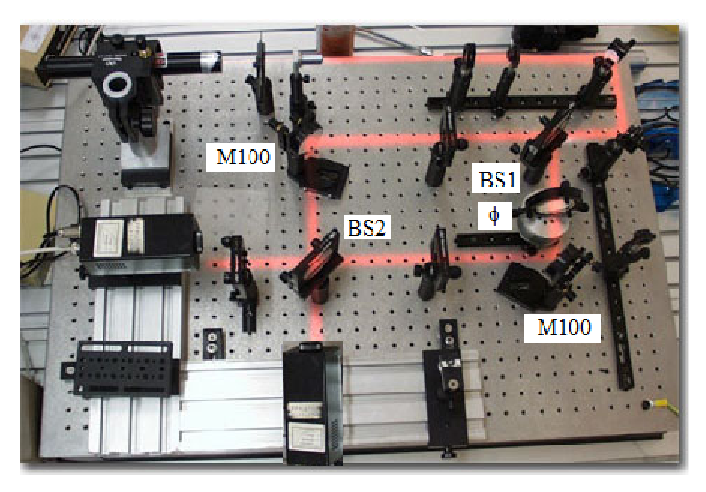
\includegraphics{graphics/MZPhaseImage.eps}%
\else
	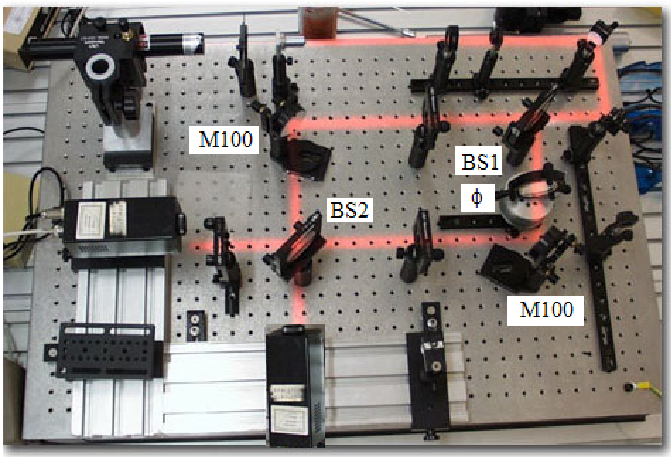
\includegraphics{graphics/MZPhaseImage.pdf}%
\fi
\end{minipage} \hfill
\begin{minipage}[c]{.30\linewidth}
\ifcase\msipdfoutput
	\includegraphics{graphics/MZPhas.eps}
\else
	\includegraphics{graphics/MZPhas.pdf}
\fi
\end{minipage}
\caption{Interféromètre de Mach-Zehnder déséquilibre (Image de laboratoire et
schéma de principe). La phase $\phi$ introduit une différence de marche ou de
longueur entre les deux bras. BS (Beam-Splitter) représente un miroir semi-
transparent. M100 est le miroir parfait.}%
\label{fig:MZPhase}%
\end{figure}

\colorbox[gray]{0.8}{
\parbox[c]{0.9\textwidth}{
\begin{definition}
Pour une expérience donnée, une \textbf{transition} est un ensemble
d'\textbf{états initiale et finale}.
\end{definition}
}}
\medskip

Dans l'expérience des fentes de Young, \emph{le passage d'un électron de la
source} $S$ \emph{pour arriver au détecteur à la position }$x$ est \textbf{une
transition}. Sur l'interféromètre de Mach-Zehnder déséquilibré, c'est par
exemple le passage d'un quanton du séparateur BS1 à un deux détecteurs.
L'objet de la théorie quantique est de prédire si cette transition a eu lieu
ou non.

On désigne par

\begin{itemize}
\item $\ket{x}$ le \textbf{vecteur d'état} qui représente \emph{le quanton qui
se propage dans la direction de }$x$;

\item $\ket{y}$ le \textbf{vecteur d'état} qui représente \emph{le quanton qui
se propage dans la direction de }$y$.
\end{itemize}

Les coefficients de réflexion $r$ et de transmission $t$ des quantons sur un
miroir semi-réfléchissant (BS) s'interprètent comme \emph{\textbf{les amplitudes
de probabilité (ou ondes de probabilité)} de réflexion et de transmission}.
Ainsi, la \textbf{probabilité} de trouver le quanton transmis par un BS unique
vaut alors $T=|t|^{2}$ et celle de le trouver réfléchi vaut $R=|r|^{2}$. Ces
probabilités doivent bien évidemment satisfaire à la \textbf{condition de
complétude}%
\begin{equation}
|t|^{2}+|r|^{2}=1.
\end{equation}
Puisque les BS de l'interféromètre de Mach-Zehnder sont équilibrés, on a, en
vertu de l'expérience MZ1,%
\begin{equation}
|t|^{2}=|r|^{2}=\frac{1}{2}\Rightarrow t=r=\frac{1}{\sqrt{2}}.
\end{equation}
Ainsi, l'action d'un BS est
\begin{equation}
\begin{cases}
\ket{x} \overset{BS}{\rightarrow}\ket{\psi_{x}} =t\ket{x}+ir\ket{y}
=\frac{1}{\sqrt{2}}(\ket{x} +i\ket{y}) \\
\ket{y} \overset{BS}{\rightarrow}\ket{\psi_{y}} =t\ket{y}+ir\ket{x}
=\frac{1}{\sqrt{2}}(\ket{y} +i\ket{x})
\end{cases}
\label{eq:ActionBS}
\end{equation}

\begin{enumerate}
\item Le facteur $i$ devant la partie réfléchie est due au fait que la
réflexion entraîne un déphasage de $\frac{\pi}{2}$ (entre le chemin incident
et le chemin réfléchi), soit un facteur de phase\footnote{En optique
ondulatoire, dans l'étude des interfaces, on suppose (hypothèse qui est
toujours formulée implicitement) que l'origine du temps sur le rayon réfléchi
est mesurée par le même observateur qui mesure le rayon incident.} $e^{i\pi
/2}=i$. Ce facteur donne un comportement symétrique aux entrées suivant $x$ et
suivant $y$.

\item $\ket{\psi_{x}}$ et $\ket{\psi_{y}}$ \emph{sont des \textbf{vecteurs
d'état} de même nature que} $\ket{x}$ et $\ket{y}$: ce sont des vecteurs
obtenu comme combinaison linéaires de deux vecteurs. Le vecteur $\ket{\psi_{x}}
$ (ou $\ket{\psi_{y}}$) décrit la \emph{\textbf{délocalisation}} du quanton
dans deux chemins indiscernables, due au BS.

\item Le principe physique correspondant à la possibilité de traiter les états
comme des vecteurs, et donc à pouvoir en prendre des combinaisons linéaires,
est appelé \textbf{principe de superposition des états.}
\end{enumerate}

Un miroir complètement réfléchissant (M100) réfléchi ou \emph{projette} un
quanton se déplaçant suivant un axe, sur l'axe orthogonal, avec une amplitude
de probabilité ou de projection $r^{\prime}$ de sorte que la probabilité de
trouver le quanton réfléchi M100 sur l'axe orthogonal est $|r^{\prime}|^{2}=1$:%
\begin{equation}%
\begin{array}
[c]{c}%
\ket{x} \overset{M100}{\rightarrow}i\ket{y}\\
\ket{y} \overset{M100}{\rightarrow}i\ket{x}
\end{array}
\end{equation}

La lame placée sur l'un des bras introduit une différence de chemin $\phi
=2\pi\frac{L}{\lambda}$ entre les deux bras qui se traduit un facteur de phase
$e^{i\phi}$, de module $1$, sur le vecteur représentant le chemin le plus
long:%
\begin{equation}
\ket{x} \overset{\phi}{\rightarrow}e^{i\phi}\ket{x}.
\end{equation}

\begin{figure}[tbh]
\centering
\ifcase\msipdfoutput
	\includegraphics{graphics/FormaMZ.eps}
\else
	\includegraphics{graphics/FormaMZ.pdf}
\fi
\caption{a) Dans un interféromètre alimenté par un champ classique,
l'intensité lumineuse $I(\varphi)$ en sortie oscille avec la différence de
phase $\varphi$ entre les deux chemins. b) Lorsqu'un photon unique est envoyé
dans l'interféromètre, la probabilité de photo-détection $P(\varphi)$ en
sortie varie avec $\varphi$ comme l'intensité qui serait obtenue pour un champ
classique. En traçant l'histogramme du nombre de photo-détections en fonction
de $\varphi$ lorsque l'expérience est répétée un grand nombre de fois, on
retrouve le système de franges attendu dans le cas classique [Après P.
Grangier \emph{et al. Europhys. Lett.,} \textbf{1}, 173 (1986)]}%
\label{fig:FormaMZ}%
\end{figure}

Ainsi, les amplitudes de probabilité ou ondes de probabilité des quatre
chemins possibles que peut emprunter le quanton envoyé suivant $x$ et détecter
après BS2 sont:%
\begin{equation}%
\begin{array}
[c]{ll}%
A(TR)=te^{i\phi}i(ir)=-tre^{i\phi} &
A(TT)=te^{i\phi}it=i|t|^{2}e^{i\phi} \\
A(RT)=(ir)it=-rt & A(RR)=(ir)i(ir)=-i|r|^{2}%
\end{array}
\label{eq:FactoAmpl1}%
\end{equation}
et les amplitudes de probabilité de détecter les quantons dans les sorties%
\begin{equation}%
\begin{array}
[c]{cc}%
x\ (TR\text{ ou }RT): & A(x)=A(TR)+A(RT)=-rt(1+e^{i\phi})=-\frac{1}%
{2}(1+e^{i\phi})\\
y\ (TT\text{ ou }RR): & A(y)=A(TT)+A(RR)=i(|t|^{2}e^{i\phi}-|r|^{2})
=\frac{i}{2}(e^{i\phi}-1)
\end{array}
\end{equation}
et les probabilités correspondantes (voir la figure \ref{fig:FormaMZ})%
\begin{equation}%
\begin{array}
[c]{c}%
\mathcal{P}(x)=|A(TR)+A(RT)|^{2}=|t|^{2}|r|^{2}|1+e^{i\phi}|^{2}%
=\frac{1}{2}(1+\cos\phi)=\cos^{2}\frac{\phi}{2}\\
\mathcal{P}(y)=|A(TT)+A(RR)|^{2}=|t|^{2}|r|^{2}|e^{i\phi}-1|^{2}%
=\frac{1}{2}(1-\cos\phi)=\sin^{2}\frac{\phi}{2}%
\end{array}
\end{equation}
On vérifie bien que
\begin{equation}
\mathcal{P}(x)+\mathcal{P}(y)=1.
\label{eq:RelCompl1}%
\end{equation}
Pour $\phi=2n\pi,$ $n\in\mathbb{N}$, tous les quantons sont détectés en $x$;
pour $\phi=(2n+1)\pi,$ $n\in\mathbb{N}$, tous les quantons sont détectés en
$y$.

\emph{\textbf{Il est donc clair que les quantons n'interfèrent jamais entre eux,
seuls interfèrent les champs ou amplitudes qui déterminent où et quand on peut
les trouver et avec quelle probabilité.}}

Cette interprétation que nous venons de faire est très générale:

\medskip
\colorbox[gray]{0.8}{
\parbox[c]{0.9\textwidth}{
\emph{il y a interférence chaque fois qu'un système physique peut prendre
plusieurs chemins distincts, pour évoluer vers un même état final, sans qu'il
soit possible, par quelque mesure que ce soit, de savoir quel chemin a été
emprunté (des chemins indiscernables). A chaque chemin est associée une
amplitude de probabilité $A$ et le carré du module de la somme de ces amplitudes
donne la probabilité $\mathcal{P}$ de trouver le système dans l'état final
considéré. Ainsi, dans un interféromètre à deux ondes comme un interféromètre de
Mach Zehnder, \textbf{ce ne sont pas les quantons qui interfèrent un à un; pour
chaque quanton, ce sont les amplitudes de probabilité associées aux deux chemins
qu'il peut prendre qui interfèrent}.}
}}

\subsection{Règles de calcul des amplitudes de probabilité}

Il apparaît que pour calculer les amplitudes de probabilités et les
probabilités quantiques, il faut définir des règles précises.

\colorbox[gray]{0.8}{
\parbox[c]{0.9\textwidth}{
\begin{definition}
\textbf{L'amplitude quantique}, qui détermine où et quand on peut trouver un
objet quantique et avec quelle probabilité, n'est définie que lorsque l'état
initial $\ket{i}$ et l'étal final $\ket{f}$ du système quantique considéré sont
spécifiés de façon unique, c'est-à-dire décrivent exhaustivement le système tout
entier. Ces états $\ket{i}$ et $\ket{f}$ définissent une \textbf{transition
quantique.}
\end{definition}
}}

\begin{enumerate}
\item L'amplitude de probabilité de la transition $f\leftarrow i$ s'écrit
\begin{subequations}
\begin{equation}
A(f\leftarrow i)=\langle f\ket{i} ,
\end{equation}
et la \textbf{probabilité} correspondante s'écrit%
\begin{equation}
\mathcal{P}(f\leftarrow i)=|\langle f\ket{i}|^{2}.
\label{eq:BornRule}
\end{equation}
La relation (\ref{eq:BornRule}) est connue sous le nom de la \textbf{règle de
Born}.
\end{subequations}
\begin{itemize}
\item Dans le dispositif des fentes d'Young (DFY), on a%
\begin{equation}
A(x\leftarrow S)=\langle x\ket{S} .
\end{equation}

\item Dans l'interféromètre de Mach-Zehnder (IMZ), partant du quanton qui se
propage suivant $S_{x}$), on a la transition quantique menant au détecteur
suivant $x$ (TR ou RT) et la transition quantique menant au détecteur suivant
$y$ (TT ou RR). On a donc%
\begin{subequations}%
\begin{align}
A(x\leftarrow S_{x})=\langle x\ket{S_{x}}\\
A(y\leftarrow S_{x})=\langle y\ket{S_{x}}
\end{align}%

\end{subequations}%

\end{itemize}

\item Pour obtenir la probabilité $\mathcal{P}(f\leftarrow i)$ d'observer
l'état final $\ket{f}$, on additionne toutes les amplitudes quantiques
conduisant au résultat $\ket{f}$ en partant de $\ket{i}$:%
\begin{equation}
A(f\leftarrow i)=\sum_{n}A_{n}(f\leftarrow i),
\end{equation}
où les amplitudes $A_{n}$ correspondent aux divers chemins physiquement
indiscernables. D'où le principe suivant:

\colorbox[gray]{0.8}{
\parbox[c]{0.9\textwidth}{
\begin{principe}
\textbf{Superposition.} On somme les amplitudes quantiques correspondant à tous
les chemins indiscernables (par exemple TR ou RT; RR ou TT) ou à des états
finaux identiques.
\end{principe}
}}

\begin{itemize}
\item Dans DFY%
\begin{subequations}%
\begin{align}
A(x\leftarrow S_{x}) &=A_{F_1}(x\leftarrow S)+A_{F_2}(x\leftarrow S),\\
\langle x\ket{S}  &  =\langle x\ket{F_1}\langle F_1\ket{S} +\langle
x\ket{F_2}\langle F_2\ket{S}.
\label{eq:PSuperp}%
\end{align}%
\end{subequations}%

\item Dans IMZ,%
\begin{subequations}%
\label{eq:Amplixy}%
\begin{align}
A(x\leftarrow S_{x}) & =A(TR)(x\leftarrow S_{x})+A(RT)(x\leftarrow S_{x})\\
\langle x\ket{S_{x}} &  =\langle x\ket{R_2}\langle R_2\ket{M_{x}}\langle
M_{x}\ket{T_1}\langle T_1\ket{S_{x}}+\langle x\ket{T_2}\langle
T_2\ket{M_{y}}\langle M_{y}\ket{R_1}\langle R_1\ket{S_{x}}\\
A(y\leftarrow S_{x}) & =A(TT)(y\leftarrow S_{x})+A(RR)(y\leftarrow S_{x})\\
\langle y\ket{S_{x}} &  =\langle y\ket{T_2}\langle T_2\ket{M_{x}}\langle
M_{x}\ket{T_1}\langle T_1\ket{S_{x}}+\langle y\ket{R_2}\langle
R_2\ket{M_{y}}\langle M_{y}\ket{R_1}\langle R_1\ket{S_{x}}
\end{align}%
\end{subequations}%

\end{itemize}

Le fait d'ajouter les amplitudes de transition intermédiaires (l'électron
passe par $F_1$ ou $F_2$ par exemple) signifie qu'\textbf{on ne peut
attribuer au quanton une trajectoire bien définie}. Cependant, quelle que soit
la position $x$ du détecteur, l'amplitude $\langle x\ket{S}
$ est \textbf{complètement déterminée} par les amplitudes de transition
\textbf{vers} et \textbf{provenant }des deux fentes, celles-ci étant les
seules transitions possibles.

La superposition d'états quantiques ouvre la voie vers des applications très
sophistiquées comme

\begin{itemize}
\item la \textbf{cryptographie quantique} qui garantirait aux utilisateurs une
intimité absolue dans leur communication grâce au \textbf{qubit},
superposition des états $\alpha_{0}\left\vert 0\right\rangle +\alpha
_1\left\vert 1\right\rangle $ qui a une infinité de valeurs alors que le
\textbf{bit} classique ne peut prendre que deux valeurs, symbolisées par $0$
et $1$;

\item la \textbf{téléportation quantique} qui permet la transmission
d'information \emph{instantanée} sur des distances illimitées;

\item l'\textbf{ordinateur quantique} dont le temps de calcul sera
radicalement inférieur comparé à celle des ordinateurs classiques actuels. On
pense qu'en superposant les états quantiques qui réalisent des opérations
parallèles simultanément, les ordinateurs quantiques peuvent rompre des codes
de chiffrement et exercer d'autres miracles technologiques impossibles avec un
ordinateur classique.
\end{itemize}

Soulignons qu'à travers la superposition des états, la cryptographie
quantique repose sur le principe d'indétermination d'Heisenberg qui induit
que\emph{\ toute mesure perturbe nécessairement l'état des électrons }. Donc
toute tentative d'interception est détectée, même si on intercepte et que l'on
réinjecte un électron dans le système après lecture.

\item Lorsqu'une transition peut se faire par des voies intermédiaires en
principe discernables, chacun de ces états peut être considéré comme final
pour une partie de la transition.

\colorbox[gray]{0.8}{
\parbox[c]{0.9\textwidth}{
\begin{principe}
\textbf{Addition des probabilités.} Lorsqu'on a pour un état initial plusieurs
états finaux différents ou disjoints, et donc plusieurs transitions quantiques,
la probabilité de transition vers l'ensemble de ces états est  la somme des
probabilités vers chacun de ces états:
\begin{equation}
\mathcal{P}(f\leftarrow i)=\sum_{n}\mathcal{P}(f_{n}\leftarrow i).
\end{equation}
\end{principe}
}}

Lorsque la somme des probabilité de transition est l'unité, on dit que ces
états forment un ensemble complet. C'est \emph{la propriété de
\textbf{complétude}} (voir l'Eq. (\ref{eq:RelCompl1})):%
\begin{equation}
\sum_{n}\mathcal{P}(f_{n}\leftarrow i)=1.
\end{equation}


\item Pour évaluer les amplitudes de l'Eq. (\ref{eq:FactoAmpl1}), nous avons
utilisé le principe suivant:

\colorbox[gray]{0.8}{
\parbox[c]{0.9\textwidth}{
\begin{principe}
\textbf{Factorisation séquentielle.} Lorsqu'une transition quantique peut se
décomposer en plusieurs \textbf{sous-transitions ou états intermédiaires},
l'amplitude de probabilité de la transition se factorise en produit des
amplitudes correspondant aux sous-transitions de la transitions:
\begin{equation}
A_{n}(f\leftarrow i)=A_{n}(f\leftarrow j)A_{n}(j\leftarrow k)\cdots
A_{n}(\ell\leftarrow i).\label{eq:PrinCFacto}\end{equation}
\end{principe}
}}

L'expression (\ref{eq:PrinCFacto}) s'énonce en lisant de droite à gauche,
puisque alors les différents états consécutifs occupés seront énoncés dans
l'ordre: état initial - état intermédiaire - état final.

Les sous-transitions ou états intermédiaires des divers transitions
indiscernables sont,

\begin{itemize}
\item dans DFY,%
\begin{subequations}%
\begin{align}
A_{F_1}(x\leftarrow S) =A_{F_1}(x\leftarrow F_1)A_{F_1}%
(F_1\leftarrow S)=\langle x\ket{F_1} \langle F_1\ket{S} ,\\
A_{F_2}(x\leftarrow S) =A_{F_2}(x\leftarrow F_2)A_{F_2}%
(F_2\leftarrow S)=\langle x\ket{F_2} \langle F_2\ket{S} ;
\end{align}%
\end{subequations}%

\item dans IMZ,
\begin{subequations}%
\begin{align}
A(TR)(x\leftarrow S_{x}) & =A(TR)(x\leftarrow R_2)A(TR)(R_2\leftarrow
M_{x})A(TR)(M_{x}\leftarrow T_1)A(TR)(T_1\leftarrow S_{x})\nonumber\\
&  =\langle x\ket{R_2}\langle R_2\ket{M_{x}}\langle M_{x}\ket{T_1}\langle
T_1\ket{S_{x}}\\
A(RT)(x\leftarrow S_{x}) & =A(RT)(x\leftarrow T_2)A(RT)(T_2\leftarrow
M_{y})A(RT)(M_{y}\leftarrow R_1)A(RT)(R_1\leftarrow S_{x})\nonumber\\
&  =\langle x\ket{T_2}\langle T_2\ket{M_{y}}\langle M_{y}\ket{R_1}\langle
R_1\ket{S_{x}}\\
A(TT)(y\leftarrow S_{x}) & =A(TT)(y\leftarrow T_2)A(TT)(T_2\leftarrow
M_{x})A(TT)(M_{x}\leftarrow T_1)A(TT)(T_1\leftarrow S_{x})\nonumber\\
&  =\langle y\ket{T_2}\langle T_2\ket{M_{x}}\langle M_{x}\ket{T_1}\langle
T_1\ket{S_{x}}\\
A(RR)(y\leftarrow S_{x}) & =A(RR)(y\leftarrow R_2)A(RR)(R_2\leftarrow
M_{y})A(RR)(M_{y}\leftarrow R_1)A(RR)(R_1\leftarrow S_{x})\nonumber\\
&  =\langle y\ket{R_2}\langle R_2\ket{M_{y}}\langle M_{y}\ket{R_1}\langle
R_1\ket{S_{x}}
\end{align}%
\end{subequations}%
où

\begin{enumerate}
\item $R_1$, $R_2$, $T_1$ et $T_2$ désignent les réflexions et les
transmissions sur $BS1$ et $BS2$;

\item $M_{x}$ et $M_{y}$ désignent respectivement les miroirs complètement
réfléchissant situés suivant $x$ et $y$ sur la figure (\ref{fig:MZPhase}).
\end{enumerate}
\end{itemize}

\item Dans (\ref{eq:PSuperp}), les termes $\langle x\ket{F_1}\langle F_2
\ket{S}$ et $\langle x\ket{F_2} \langle F_1\ket{S} $ sont implicitement
nuls. En effet, quelle est l'amplitude de transition pour qu'un électron parte
de $S$, passe par la fente $F_1$ (resp. $F_2$), sorte par la fente $F_2$
(resp. $F_1$)? La réponse à cette question devrait inclure la transition de
la fente $F_1$ (resp. $F_2$) à la fente $F_2$ (resp. $F_1$), i.e.,
l'amplitude $\langle F_1\ket{F_2} $ (resp.$\langle F_2\ket{F_1} $):%
\begin{equation}
\langle x\ket{F_1} \langle F_1\ket{F_2} \langle F_2\ket{S} \text{ ou
}\langle x\ket{F_2} \langle F_2\ket{F_1} \langle F_1\ket{S} .
\end{equation}
Cependant, on peut vérifier expérimentalement qu'on ne peut détecter un
électron qui entre par une fente et qui sort par une autre fente. Ainsi, les
transitions quantiques observées présentent la \emph{propriété de
\textbf{disjonction mutuelle}:}%
\begin{equation}
\langle F_1\ket{F_2} =\langle F_2\ket{F_1} =0.
\end{equation}
Signalons aussi que \emph{l'amplitude de transition (et la probabilité) entre
un état initial et un état final identiques est égale à l'unité:}%
\begin{subequations}%
\begin{align}
\langle F_1\ket{F_1} =\langle F_2\left\vert
F_2\right\rangle =1,\\
\mathcal{P}(i\leftarrow i)=1.
\end{align}%
\end{subequations}%

\item Si on considère un ensemble disjoint et complets d'états $f_{n}$, on
peut écrire%
\begin{subequations}%
\begin{align}
1  &  =\langle i\ket{i} =\sum_{n}\langle i\ket{f_{n}}\langle f_{n}\ket{i} \\
1  &  =\sum_{n}\mathcal{P}(f_{n}\leftarrow i)=\sum_{n}|\langle
f_{n}\ket{i}|^{2}%
\end{align}%
\end{subequations}%
Ces relations suggèrent que%
\begin{equation}
\langle f_{n}\ket{i} =\langle i\ket{f_{n}}^{\ast}.
\end{equation}
\colorbox[gray]{0.8}{
\parbox[c]{0.9\textwidth}{
\emph{D'où la \textbf{règle de conjugaison des amplitudes de probabilité
quantiques}: les amplitudes de probabilité quantiques de deux transitions
inverses l'une de l'autre sont complexes conjuguées}
\begin{equation}
\langle f\ket{i} =\langle i\ket{f}^{\ast }\text{ ou }A(f\leftarrow
i)=A^{\ast}(i\leftarrow f).\label{eq:ReglConjug}
\end{equation}
\emph{La conséquence immédiate est la \textbf{symétrie des probabilités:} les
probabilités des deux transitions quantiques inverses sont égales}
\begin{equation}
\mathcal{P}(f\leftarrow i)=\mathcal{P}(i\leftarrow f).
\end{equation}
}}
\medskip

Soulignons que
\begin{equation}
|\langle f\ket{i} |^{2}=\langle f\ket{i} ^{\ast}\langle f\ket{i}
=\langle i\ket{f}\langle f\ket{i} .
\end{equation}
Ainsi, en vertu de l'Eq. (\ref{eq:Amplixy}), on a%
\begin{subequations}%
\begin{align}
\mathcal{P}(x\leftarrow S_{x}) & =|\bra{x}S_{x}\rangle|^{2}=|A(TR)(x\leftarrow
S_{x})|^{2}+|A(RT)(x\leftarrow S_{x})|^{2}\nonumber\\
&  \left.  +A(TR)^{\ast}(x\leftarrow S_{x})A(RT)(x\leftarrow S_{x})
+A(RT)^{\ast}(x\leftarrow S_{x})A(TR)(x\leftarrow S_{x})\right. \\
\mathcal{P}(y\leftarrow S_{x}) & =|\bra{y}S_{x}\rangle|^{2}=|A(TT)(y\leftarrow
S_{x})|^{2}+|A(RR)(y\leftarrow S_{x})|^{2}\nonumber\\
&  \left.  +A(TT)^{\ast}(y\leftarrow S_{x})A(RR)(y\leftarrow S_{x}%
)+A(RR)^{\ast}(y\leftarrow S_{x})A(TT)(y\leftarrow S_{x})\right.
\end{align}%
\end{subequations}
Les produits $A(TR)^{\ast}(x\leftarrow S_{x})A(RT)(x\leftarrow S_{x})$,
$A(RT)^{\ast}(x\leftarrow S_{x})A(TR)(x\leftarrow S_{x})$, $A(TT)^{\ast
}(y\leftarrow S_{x})A(RR)(y\leftarrow S_{x})$ et $A(RR)^{\ast}(y\leftarrow
S_{x})A(TT)(y\leftarrow S_{x})$ sont les \textbf{termes d'interférences
quantiques.}

C'est donc à la superposition des amplitudes de probabilité et la règle de
conjugaison des amplitudes de probabilité quantiques qu'on doit les figures
d'interférence.

\medskip\colorbox[gray]{0.8}{
\parbox[c]{0.9\textwidth}{
\emph{Quand on dit que chaque quanton interfère avec lui-même, il
s'agit en fait d'interférences d'amplitudes de probabilité.}
}}
\end{enumerate}

Achevons ce chapitre, porte d'entrée dans le merveilleux monde quantique, en
notant que classiquement, on est habitué à un \emph{déterminisme} rigide et à la
relation de \emph{causalité}: quand on connaît les conditions initiales, on sait
parfaitement ce qui va se passer. En théorie quantique, ces certitudes sont
abandonnées. La possibilité de prévoir le comportement d'un système quantique
n'est qu'une prédictibilité probabiliste (un seul événement) et statistique
(grand nombre d'événements). L'objet quantique est en quelque sorte une
\emph{juxtaposition de possibles}: on parle d'\emph{indéterminisme}. On dit
aussi que \emph{Dieu joue au dés en théorie quantique}\footnote{Einstein n'a
jamais accepter le caractère probabiliste lié à la discontinuité des quanta
alors même qu'il avait prouvé en 1905 l'existence des atomes à partir d'une
interprétation probabiliste des fluctuations d'entropie dans le mouvement
brownien.}.

\medskip
\colorbox[gray]{0.8}{
\parbox[c]{0.9\textwidth}{
\emph{Tant que la mesure sur lui n'est pas faite, la grandeur censée quantifier
la propriété physique recherchée n'est pas strictement définie. Mais dès que
cette mesure est engagée, elle détruit la superposition quantique.}
}}

\subsection{Chat de Schrödinger}
\label{sec:EtatSuper}

Nous avons déjà annoncé la fin du chapitre, alors pourquoi cette section? Eh
bien, pour raconter une histoire au coin du feu!

C'est l'histoire du fameux du \textbf{paradoxe du chat de Schrödinger} dont
nous avons fait allusion à la \textbf{section \ref{sec:InterfMZ}}.

En effet, dans les années $1930$, ce célèbre physicien Autrichien avait, en
pensée, enfermé un chat dans une boîte en acier contenant un flacon de gaz
mortel, un compteur de radioactivité et un atome radioactif. Si le compteur
détecte de la radioactivité, un mécanisme casse le flacon, et le chat meurt. Le
compteur, appareil macroscopique, ne peut que mesurer l'un des deux états
classiques possibles de l'atome: \emph{désintégré} et \emph{non-désintégré}. On
suppose qu'après un temps $t_{1/2}$, l'atome se désintègre avec une probabilité
(quantique) $\frac{1}{2}$ (voir la figure \ref{fig:SchoedingerCat}). Tant
qu'aucune mesure n'est effectuée, cet atome se trouve dans un état superposé, à
la fois \emph{désintégré} et \emph{non-désintégré}. Par conséquent, tant que la
boîte reste fermée, le chat est dans un \textbf{état superposé}, \textbf{à la
fois mort et vivant}! Attention, le chat \textbf{n'est pas mort-vivant}, il est
soit mort, soit vivant, mais tant que la boîte n'est pas ouverte, notre
information sur son état est nécessairement constituée de ces deux possibilités.
C'est en l'observant que l'on constate que le chat est mort ou vivant. Donc, on
réduit le paquet d'ondes, transformant le chat de l'état superposé
$\frac{1}{\sqrt{2}}(\ket{vivant} + \ket{mort})$ à l'état $\ket{vivant}$ ou
$\ket{mort}$\footnote{En fait il n'y a pas paradoxe, puisque le principe de
superposition n'est valable que pour les états quantiques. Or le chat est
macroscopique.}.

\begin{figure}[ptbh]
\centering
\ifcase\msipdfoutput
  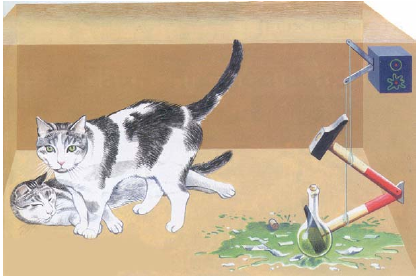
\includegraphics[scale=.8]{graphics/SchoedingerCat.eps}
\else
  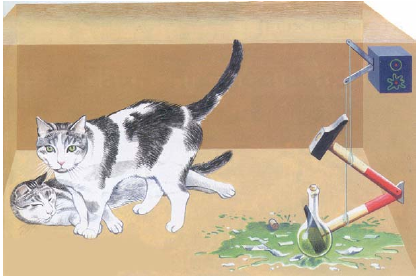
\includegraphics[scale=.8]{graphics/SchoedingerCat.png}
\fi
\caption{Le chat de Schrödinger dans la boîte d'acier. Tant que boîte reste
fermé, le chat est dans un état superposé mort et vivant.}
\label{fig:SchoedingerCat}
\end{figure}

Soulignons que depuis quelques années, la tendance en électronique quantique
est plutôt d'utiliser les mots \emph{chat de Schrödinger} d'une façon
différente, pour caractériser une superposition cohérente de possibilités
macroscopiquement distinctes. La cohérence du chat est évidemment une
condition suffisante pour qu'il soit dans un état flou à la Schrödinger (la
superposition cohérente sous entend nécessairement l'existence des deux
possibilités); mais elle n'est pas nécessaire.

Achevons cette histoire au coin du feu en nous demandant si le chat peut être
considéré comme un observateur: \emph{le chat peut-il avoir conscience d'être
mort ou vivant?} Le chat ne peut avoir conscience par définition que d'être
vivant. Cependant, cela ne l'empêche pas de constituer un observateur
acceptable: vivant, il peut laisser dans la boîte des traces de son état, mort,
il laisse d'autres types de traces, de sorte que la \emph{mesure} de son état
vivant ou mort serait également l'inscription rétroactive (en remontant le temps
!) des traces laissées.
\bigskip

\emph{Wolai!! Effectuer la mesure dans le monde quantique est une histoire
compliquée!!}

\begin{remark}

\begin{small}
Bien que le dispositif de Schrödinger soit, il a l'intérêt de mettre en
évidence, qu'en principe au moins, l'étrangeté quantique des systèmes
microscopiques se communique aux systèmes macroscopiques. Et il pose une
question de fond: \emph{pourquoi les gens ne voient-ils que des chats soit
vivants, soit morts et pas de chats morts-vivants?}

D'après la vision actuelle, si le monde semble si bien décrit par la physique
classique, c'est parce que les interactions complexes d'un objet avec son
environnement font très vite disparaître les particularités quantiques.
L'information relative à l'état de santé d'un chat, par exemple, gagne
rapidement son environnement sous la forme de photons et d'échanges de chaleur.
Chaque phénomène quantique peut impliquer des états superposés du système en jeu
(mort ou vivant), mais ces états tendent à disparaître. La fuite permanente
d'information vers l'environnement est le mécanisme essentiel par lequel les
états quantiques de superposition se détruisent, processus nommé
\textbf{décohérence}. Les gros systèmes sont davantage sujets à la décohérence
que les petits, tout simplement parce qu'ils laissent échapper plus
d'informations. C'est pourquoi les physiciens tendent à associer la théorie
quantique au monde microscopique. Dans de nombreux cas, toutefois, la perte
d'information par un gros système peut être ralentie ou stoppée, ce qui met
alors en évidence l'omniprésence des phénomènes quantiques.
\end{small}

\end{remark}

\newpage

\section{Exercices et problèmes}

\subsection{Interféromètre de Mach-Zehnder à deux lames}
\begin{figure}[ptbh]
\centering
	\ifcase\msipdfoutput
		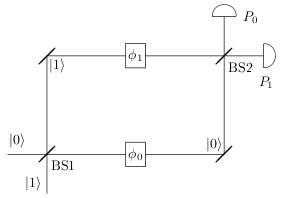
\includegraphics[scale=.8]{graphics/InterferometreEkert.eps}%
	\else
		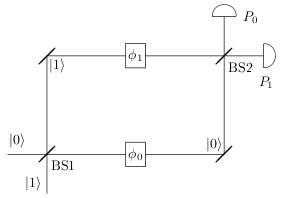
\includegraphics[scale=.8]{graphics/InterferometreEkert.jpg}%
	\fi
\caption{MZ à deux lames.}
\label{fig:MZ2Lames}
\end{figure}

On considère l'interféromètre de la figure \ref{fig:MZ2Lames}. Le quanton qui y
pénètre est soit dans l'état $ \ket{0}$, soit dans l'état $\ket{1}$. Quelles
sont les probabilités $\mathcal{P}_{0}$ et $\mathcal{P}_1$ ce quanton aux
détecteurs $D_{0}$ et $D_1$?

\subsection{Amplitudes de probabilité de transition}

\begin{figure}[ptbh]
\centering
\begin{minipage}[c]{.6\linewidth}
	\ifcase\msipdfoutput
		\includegraphics[scale=.8]{graphics/DispoYoung.eps}%
	\else
		\includegraphics[scale=.8]{graphics/DispoYoung.pdf}%
	\fi
\caption{Dispositif des fentes d'Young. Les fentes $F_1$ et $F_2$ sont à
la même distance $r_{0}$ de la source $S$.}%
\label{fig:DispoYoung}%
	\end{minipage} \hfill\begin{minipage}[c]{.38\linewidth}
	\ifcase\msipdfoutput
		\includegraphics{graphics/FigInterfPhotons.eps}%
	\else
		\includegraphics[scale=.9]{graphics/FigInterfPhotons.pdf}%
	\fi
\caption{Figure d'interférences photon par photon [École Normale Supérieure de
Cachan (France, 2005)].}%
\label{fig:FigInterfPhotons}%
\end{minipage}
\end{figure}

Pour un photon d'énergie bien définie, $E=\hbar\omega$, l'amplitude de
probabilité de transition d'un point $A$ à un point $B$ est donnée par:%
\begin{equation}
\langle B\ket{A}=\varphi(AB)e^{-i\omega t},
\label{eq:AmplAB}%
\end{equation}
où $t$ est le temps de parcours et $\varphi(AB)$ est une fonction qui dépend
uniquement de la distance entre les points $A$ et $B$. Dans le cas où la
divergence d'un faisceau de lumière peut être négligée tous les photons
partant de $A$ arrivent en $B$. La probabilité de transition pour un photon
est égale à l'unité. L'amplitude de probabilité est alors de la forme:%
\begin{equation}
\langle B\ket{A}=e^{i\alpha}e^{-i\omega t},
\end{equation}
L'amplitude étant indéterminée à un facteur de phase près on peut poser
$\alpha=0$.

Grâce à un dispositif spécial, la source $S$ ne produit que des photons
uniques qui passent soit par $F_1$, soit par $F_2$ et peuvent être
détectés au point $X$ (voir la figure \ref{fig:DispoYoung}). Il existe deux
chemins en principe indiscernables.

\begin{enumerate}
\item Appliquer le principe de superposition pour exprimer l'amplitude de
probabilité $\ket{\psi} =\langle X\ket{S}$ du photon détecté au point $X$.
Expliciter cette expression à l'aide du principe de factorisation séquentielle.
En déduire l'expression de la probabilité $\mathcal{P}(X\leftarrow S)$ pour
qu'un photon émis par la source $S$ arrive en $X$ en passant par l'une ou
l'autre fente en faisant apparaître explicitement les termes
d'\emph{interférences quantiques}, en supposant que les amplitudes de
probabilité de transition de la source $S$ aux fentes $F_1$ et $F_2$ sont
les mêmes.

\item Soient $t_{0}$ le temps de parcours de la source à l'une des fentes,
$t_1$ le temps de parcours de la fente $F_1$ au point $X$, $t_2$ le
temps de parcours de la fente $F_2$ au point $X$. Exprimer, en vertu de
l'Eq. (\ref{eq:AmplAB}), chaque amplitude de probabilité de transition
intermédiaire en fonction $r_{i}$ et $t_{i}$ et en déduire l'expression de
$\ket{\psi} $.

\item Aux grandes distances, c'est-à-dire lorsque $r_1$ et $r_2$ sont
beaucoup plus grands que la distance entre des fentes les amplitudes
$\varphi(r_1)$ et $\varphi(r_2)$ sont à peu près égales et on peut écrire
$\varphi(r_1)=\varphi(r_2)=C^{\prime}$. Montrer que la probabilité pour
qu'un photon émis par la source $S$ arrive en $X$ en passant par l'une ou
l'autre fente est de la forme%
\begin{equation}
\mathcal{P}(X\leftarrow S)=2|C|^{2}\left[1+\cos\frac{\omega}{c}(r_2-r_1)
\right].
\end{equation}


\item Pour quelles valeurs de la différence de marche $r_2-r_1$, en
fonction de $\lambda$, a-t-on les franges brillantes et des franges sombres
(voir la figure (\ref{fig:FigInterfPhotons}))?
\end{enumerate}

\subsection{Chat de Schrödinger}

Nous reprenons dans cette exercice, la célèbre expérience de pensée de
Schrödinger en considérant un chat enfermé dans une boîte avec un poison
(substance radioactive) qui va déclencher la mort du chat à un moment ou un
autre. Classiquement, le chat est soit mort, soit vivant. Quantiquement, on
dit que le chat est dans une \emph{superposition d'états mort ou vivant.}

\begin{enumerate}
\item Quelle base conceptuelle de la physique classique se trouve remise en
cause par cette expérience?

\item On se place dans la situation quantique. On désigne l'état mort et
l'état vivant par les kets respectifs $\ket{m}$ et $\ket{v}$.

\begin{enumerate}
\item Exprimer dans la base $\{\ket{m},\ket{v}\} $ un état quelconque
$\ket{\psi}$ du chat.

\item Quelle condition doit être remplie pour que cet état traduise une onde
de probabilité?

\item Quels sont les deux états \emph{limites}? Quand les obtient-on?

\item Soit $t_1$ le temps au bout duquel le chat a une chance sur deux d'être
vivant et $t_2$ celui au bout duquel il a une chance sur quatre d'être vivant.
Exprimer les états $\ket{\psi_1}$ et $\ket{\psi_2}$ du chat correspondant à
ces instants.
\end{enumerate}
\item En utilisant QuTiP, représenter sur une sphère de Bloch les états 
$\ket{m}$, $\ket{v}$, $\ket{\psi_1}$ et $\ket{\psi_2}$.
\end{enumerate}



\chapter{Mesure et opérateurs linéaires}
\label{sec:OpLin}
\minitoc

\bigskip


Maintenant que nous sommes entré dans le monde quantique, il est légitime de se
demander comment on y extrait l'information ou comment on y effectue la mesure
sur un système. On le fait  grâce aux \textbf{opérateurs}  qui sont des
représentations mathématiques, des grandeurs physiques (\textbf{section
\ref{sec:MesGrPh}}). L'essentiel de ce chapitre, très mathématique, est donc
consacrée à l'algèbre des opérateurs linéaires (\textbf{section \ref{sec:OOL}})
et à l'étude des propriétés des opérateurs hermitiens, opérateurs associés aux
grandeurs physiques (\textbf{section \ref{sec:DSO}}).

\section{Mesure de grandeurs physiques et opérateurs}
\label{sec:MesGrPh}

La théorie quantique est avant tout une théorie des phénomènes microscopiques ou
plus exactement nanoscopiques ($10^{-9}$). Mais la physique est macroscopique
(les microscopes, accélérateurs de particules, etc., sont des objets
macroscopiques), et il est donc indispensable que les résultats simples de la
théorie classique puissent se retrouver en théorie quantique. D'autre part,
contrairement à la situation classique, il y a \textbf{indéterminisme} dans la
mesure, vu que nous ne saurons dire \textbf{exactement} où est passé le quanton
lorsqu'on observe une interférence avec des fentes de Young ou un interféromètre
de Mach Zehnder. De ce fait, il est donc important de se munir d'une théorie de
la mesure, afin d'éviter de transposer au monde nanoscopique notre expérience
journalière qui est macroscopique\footnote{Mais où est la limite entre le monde
macroscopique et le monde microscopique?}.

\colorbox[gray]{0.8}{
\parbox[c]{0.9\textwidth}{
\begin{definition}
\emph{\textbf{Une mesure est le résultat d'une interaction temporaire entre le
système et un appareil de mesure} }(qui peut être un homme). Or comme il y a
un quantum d'action minimale, $\frac{\hbar}{2}$ \textbf{(il y a un minimum de
changement dans la nature)}, on ne peut éviter que l'observation influence ou
perturbe le système quantique. C'est pourquoi toute description précise de
l'observation doit inclure une description de cette perturbation qui est
modélisée par un changement d'état.
\end{definition}
}}\medskip

\subsection{Mesure de grandeurs physiques}
\label{sec:ExpSG}

Reprenons le chemin du laboratoire où d'une source nous faisons sortir un jet
monocinétique d'atomes électriquement neutres argent (Ag), paramagnétiques,
porteurs d'un moment magnétique intrinsèque de spin. Nous avons ainsi préparer
$N$ quantons indépendamment dans le même état $\ket{\psi}$. Ces atomes
traversent l'entrefer d'un aimant où règne un fort gradient d'induction
magnétique $\frac{\partial B}{\partial z}$. Chaque atome est alors soumis à une
force $F_{z}=\mu_{z}\frac{\partial B}{\partial z}$, où $\mu_{z}$ est la
projection du moment magnétique de spin de l'atome sur le vecteur unitaire
$\bls{z}$. Lorsque l'induction magnétique est nulle, on observe, sur une
plaque de verre placée perpendiculairement au jet à une certaine distance de la
sortie de l'entrefer, une tache unique de dimension finie en raison de la
dispersion des vitesses. En présence du gradient d'induction magnétique, la
théorie classique prévoit un élargissement de la tache précédente du fait de
l'orientation à priori aléatoire des moments magnétiques $\bls{\mu}$ lors
de la production des atomes\footnote{Les atomes de moment magnétique
$\bls{\mu}$ antiparallèle à $Oz$ devraient subir une déviation maximale
vers le haut pour $\frac{\partial B}{\partial z}<0$. Ceux de $\bls{\mu}$
parallèle à $Oz$, une déviation maximale vers le bas. Toutes les déviations
intermédiaires étant possibles.}.

\begin{figure}[ptbh]
\centering
\ifcase\msipdfoutput
  \includegraphics{graphics/SternGerlachExper.eps}
\else
  \includegraphics{graphics/SternGerlachExper.pdf}
\fi
\caption{Expérience de Stern et Gerlach: classiquement, on devrait avoir une
tache unique de dimension finie, mais on observe plutôt deux taches
symétriques d'égales intensités aux points $(z_{+})$ et $(z_{-})$.}%
\label{fig:SternGerlachExper}%
\end{figure}

Cependant, on observe (voir la figure \ref{fig:SternGerlachExper}), que les
impacts des atomes, pourtant identiques, se répartissent en deux taches
quasi-ponctuelles d'égales intensités $I_{+}$ et $I_{-}$ (de moment magnétique
de spin $\mu_{+}=+\frac{\hbar}{2}$ et $\mu_{-}=-\frac{\hbar}{2}$), de part et
d'autre du point d'impact en absence d'induction magnétique, à égale distance,
i.e., $\mathcal{P}_{+}=\mathcal{P}_{-}=\frac{1}{2}$. On notera $\ket{+}$
(\emph{up}) et $\ket{-}$ (\emph{down}) l'état des atomes de moment magnétique de
spin $\mu_{+}=+\frac{\hbar}{2}$ et $\mu_{-}=-\frac{\hbar}{2}$.

Il apparaît que l'appareil de Stern et Gerlach instaure une \emph{corrélation}
dans le faisceau émergent entre l'état de spin et sa situation spatiale. On
reconnaît alors un spin \emph{up} à ce qu'il a comme point d'impact la position
$(z_{+})$ et un spin \emph{down} à ce qu'il y a comme point d'impact la position
$(z_{-})$. La distance entre ces deux points étant proportionnelle au gradient
$\frac{\partial B}{\partial z}$. Ainsi, un atome initialement dans un état de
spin quelconque $\left\vert \psi \right\rangle $ (orientation des moments
magnétiques \emph{à priori} quelconque), donne après une mesure de la
\textbf{grandeur physique spin} $\mathcal{S}$, une valeur
$\mu_{+}=+\frac{\hbar}{2}$ ou $\mu_{-}=-\frac{\hbar }{2}$, signifiant
qu'\emph{après la mesure} l'atome est dans l'état $\ket{+}$ ou $\ket{-}$. Ainsi,
\textbf{\emph{lors de son interaction avec l'appareil de mesure, le quanton
change d'état}}. On dit qu'il y a \textbf{réduction du paquet d'ondes},
autrement, \textbf{la mesure a perturbé le système}. \emph{\textbf{Cette
réduction force l'émergence classique d'un résultat unique.}}

\colorbox[gray]{0.8}{
\parbox[c]{0.9\textwidth}{
\begin{principe}\textbf{Réduction du paquet d'ondes.} Après une mesure sur un
système quantique, on modifie en général l'état de ce système.
\end{principe}
}}\medskip

L'ensemble $\{\mu_{+},\mu_{-}\}$ est l'ensemble \textbf{complet } des résultats
de la mesure de $\mathcal{S}$ puisque ce sont les seules modalités qu'on peut
obtenir lors de cette mesure. Cet ensemble complet de résultats est obtenu avec
$N$ atomes paramagnétiques dans le même état $\ket{\psi} $. Donc \emph{avant la
mesure}, le système est dans l'état superposé (exploration de tous les chemins
possibles)
\begin{equation}
\ket{\psi} =\sum_{i}\ket{i}\langle i\ket{\psi} =\alpha_{+}\ket{+}+\alpha_{-}
\ket{-}.
\end{equation}
Les amplitudes $\alpha_{\pm}=\langle\pm\ket{\psi}$ décrivent
l'\emph{orientation} du spin dans l'espace tridimensionnel: ce sont des
\emph{coordonnées ou amplitudes de projections} dans la base des états de spin
$\{\ket{+},\ket{-}\}$.

Du point de vue classique, cette situation est paradoxale puisque le
comportement de chaque atome ne peut être prédit, bien qu'il soit tous
préparés de la même façon et indépendamment. \emph{Dans chaque atome
individuel, il existe l'alternative dichotomique d'être dans l'état spin up ou
spin down}.

Les probabilités d'obtenir les moments magnétiques de spin $\mu_{+}$ et
$\mu_{-}$ sont donc%
\begin{equation}
\mathcal{P}_{+}=|\langle+\ket{\psi} |^{2}=|\alpha_{+}|^{2}\text{ et
}\mathcal{P}_{-}=|\langle-\ket{\psi}|^{2}=|\alpha_{-}|^{2},
\end{equation}
avec
\begin{equation}
\alpha_{+}=\alpha_{-}=\frac{1}{\sqrt{2}}.
\end{equation}
Par suite, la probabilité totale est (complétude du système)%
\begin{equation}
\mathcal{P}=|\alpha_{+}|^{2}+|\alpha_{-}|^{2}=1.
\end{equation}

L'effet de l'appareil de mesure est décrit par l'\textbf{opérateur} $S$ qui
opère sur l'état $\ket{\psi} $ pour donner $\ket{+}$ ou $\ket{-}$, \textbf{états
propres} de $S$ avec les \textbf{valeurs propres} $+\frac{\hbar}{2}$ ou
$-\frac{\hbar}{2}$:%
\begin{equation}
S\ket{\psi} =\begin{cases}
+\frac{\hbar}{2}\ket{+},\\
\text{ou}\\
-\frac{\hbar}{2}\ket{-}.
\end{cases}
\end{equation}
On dit que l'opérateur transforme un vecteur d'état de l'espace de Hilbert en
un autre vecteur d'état du même espace de Hilbert.

\medskip\colorbox[gray]{0.8}{
\parbox[c]{0.9\textwidth}{
\emph{Autrement, le lien entre ce qu'on peut observer du système, une grandeur
physique $\mathcal{A}$, et le système, se fait à travers le lien entre
l'opérateur $A$ associé à cette grandeur physique et le vecteur d'état.}
}}
\medskip

Autant que possible, nous utiliserons des lettres majuscules (droites) pour
les opérateurs.%

\subsection{Autres Expériences}

\begin{figure}[ptbh]
\centering
\ifcase\msipdfoutput
	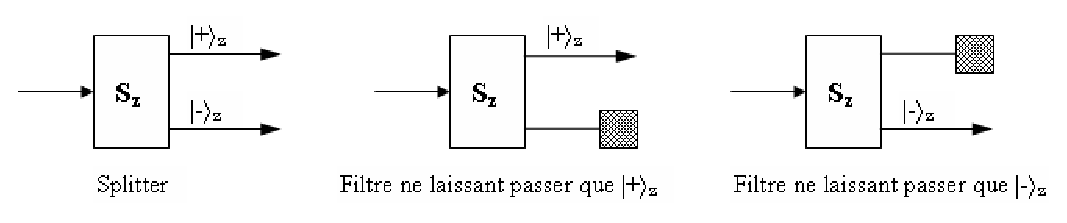
\includegraphics[scale=.9]{graphics/SGSplitterFiltre.eps}
\else
	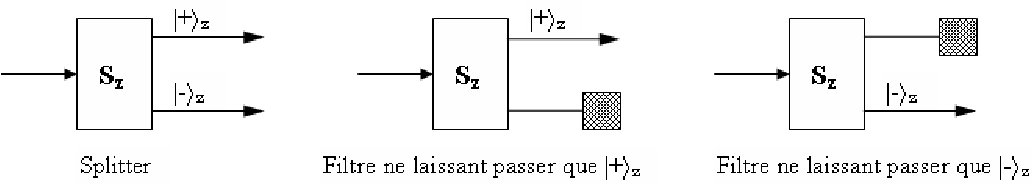
\includegraphics[scale=.9]{graphics/SGSplitterFiltre.pdf}
\fi
\caption{Stern et Gerlach comme séparateur du jet atomique ou splitter et comme
filtres.}%
\label{fig:SGsplitterFiltre}%
\end{figure}

Nous allons maintenant réaliser diverses expériences sur le spin en utilisant
les symboles de la figure \ref{fig:SGsplitterFiltre} pour les divers rôles des
appareils de Stern et Gerlach.

\subsubsection{Première expérience SG1}

A la sortie du filtre de la figure \ref{fig:sgszsz}, chaque atome est dans
un état propre de l'opérateur $S_{z}$ que l'on mesure. Le résultat de la
mesure est donc \textbf{certain}: on trouve à coup sûr la valeur propre
correspondante $+\frac{\hbar}{2}$%
\begin{equation}
\mathcal{P}(+\frac{\hbar}{2})=|\langle+\ket{+}|^{2}=1.
\end{equation}

\begin{figure}[ptbh]
\begin{minipage}[c]{.48\linewidth}
\centering
\ifcase\msipdfoutput
	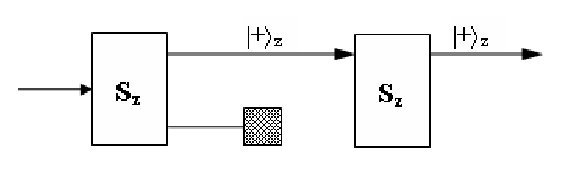
\includegraphics[scale=.8]{graphics/SGSzSz.eps}
\else
	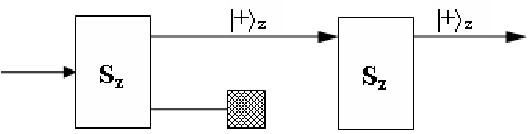
\includegraphics[scale=.8]{graphics/SGSzSz.pdf}
\fi
\caption{Mesure de $\mathcal{S}_{z}$ dans l'état $\ket{+}$.}%
\label{fig:sgszsz}%
\end{minipage} \hfill
\begin{minipage}[c]{.48\linewidth}
\centering
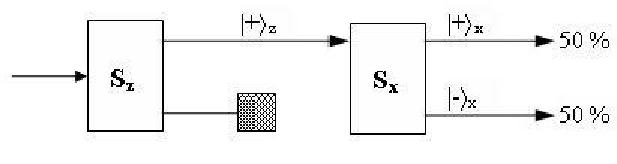
\includegraphics[scale=.8]{graphics/SGSzSx.pdf}
\caption{Mesure de $\mathcal{S}_{x}$ dans l'état $\ket{+}$.}%
\label{fig:sgszsx}%
\end{minipage}
\end{figure}


\subsubsection{Deuxième expérience SG2}

A la sortie du filtre de la figure \ref{fig:sgszsx}, chaque atome qui entre
dans le splitter orienté dans la direction $Ox$ est dans l'état $\ket{+}$. Lors
du processus de mesure de la grandeur $\mathcal{S}_{x}$, \textbf{il y a
indétermination dans le comportement de chaque atome} puisque $\ket{+}$
\emph{n'est pas un état propre de l'opérateur} $S_{x}$. Cet
opérateur à pour valeurs propres $+\frac{\hbar}{2}$ et $-\frac{\hbar}{2}$
associées respectivement aux états propres $\ket{+}_{x}$ et
$\ket{-}_{x}$. C'est parce que $\ket{+}$ se projette dans la base $\{
\ket{+}_{x},\ket{-}_{x}\}$ qui diagonalise $S_{x}$ qu'on observe à la sortie
deux faisceaux d'égales intensités, i.e.,

\begin{enumerate}
\item un faisceau où les atomes ont un spin $+\frac{\hbar}{2}$ avec la
probabilité $|_{x}\langle+\ket{+}|^{2}=\frac{1}{2}$;

\item un faisceau où les atomes ont un spin $-\frac{\hbar}{2}$ avec la
probabilité $|_{x}\langle-\ket{+}|^{2}=\frac{1}{2}$.
\end{enumerate}

\subsubsection{Troisième expérience SG3}

\begin{figure}[ptbh]
\centering
\ifcase\msipdfoutput
	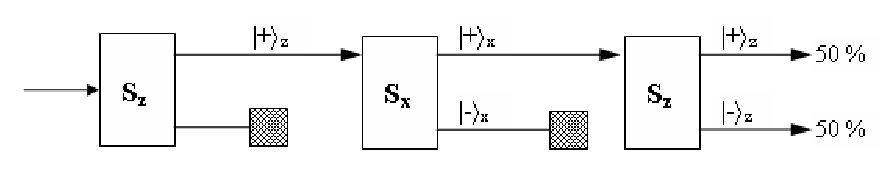
\includegraphics[scale=.9]{graphics/SGSzSxSzP.eps}
\else
	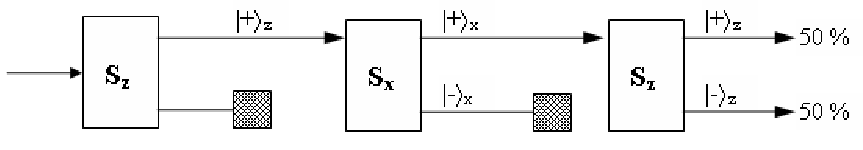
\includegraphics[scale=.9]{graphics/SGSzSxSzP.pdf}
\fi
\caption{Incompatibilité des mesures de $\mathcal{S}_{z}$ et $\mathcal{S}_{x}$.}
\label{fig:sgszsxszp}%
\end{figure}

On filtre maintenant $\ket{+}$ que fait pénétrer dans $S_{x}$. On filtre la
sortie de ce SG pour ne laisser sortir que $\ket{+}_{x}$ qui va pénétrer dans
un $S_{z}$. On constate avec surprise qu'on a à la sortie des atomes dans les
états propres $\ket{+}$ et $\ket{-}$ de $S_{z}$, alors que $\ket{-}$ a été
exclus à la sortie du premier SG, $S_{z}$.

Cette expérience met en exergue le fait qu'en théorie quantique, \emph{l'état
final du système dépend seulement de l'état de l'atome qui entre dans le dernier
SG et de son action avec cet appareil}. Autrement, il n'y a pas de mémoire sur
l'histoire passée du système.

En clair, comme le faisceau qui entre dans le dernier SG, $S_{z}$ est dans
l'état  $\ket{+}_{x}$ qui n'est pas état propre de $S_{z}$, il va se projeter
dans la base  \{$\ket{+},\ket{-}\}$ des états propres de $S_{z}$. C'est
pourquoi on a

\begin{enumerate}
\item un faisceau où les atomes ont un spin $+\frac{\hbar}{2}$ avec la
probabilité $|\langle+\ket{+}_{x}|^{2}=\frac{1}{2}$;

\item un faisceau où les atomes ont un spin $-\frac{\hbar}{2}$ avec la
probabilité $|\langle-\ket{+}_{x}|^{2}=\frac{1}{2}$.
\end{enumerate}

\subsection{Point sur la mesure}

Il découle de ce qui précède que:

\begin{enumerate}
\item L'acte de mesure modifie généralement d'une manière \emph{instantanée}
le système de façon \emph{irréversible}: c'est \textbf{la réduction du paquet
d'onde}.

\item \textbf{Le résultat complet de la mesure expérimentale} de la grandeur
physique $\mathcal{A}$ sur le système consiste à déterminer les modalités
$a_{i}$ (résultats de la mesure) et les amplitudes de probabilité $\alpha_{i}$
ou les probabilités $\mathcal{P}_{i}=|\alpha_{i}|^{2}$. Autrement dit, il s'agit
d'extraire des nombres contenus dans le vecteur d'état $\ket{\psi}$.

\item Les modalités $a_{i}$ dépendent de la \emph{nature} du système et les
amplitudes de probabilité $\alpha_{i}$ dépendent de l'\emph{état} du système
ou du vecteur d'état $\ket{\psi}$.

\item L'\textbf{opérateur} $A$ extrait de $\ket{\psi}$ l'information physique
sur la grandeur physique $\mathcal{A}$. $\ket{\psi}$ décrit la réalité physique
d'un système quantique individuel.

\item Lorsqu'on a \emph{un seul} système dans l'état $\ket{\psi}$, si \emph{une
seule} mesure de $\mathcal{A}$ donne la modalité $a_{i},$ le système est après
cette mesure dans l'état $\ket{\varphi_{i}}$ associé à $a_{i}$%
\begin{equation}
\ket{\varphi_{i}}=\ket{A\psi}=A\ket{\psi} ,
\end{equation}
$A$ est l'\emph{opérateur (hermitien)\footnote{Les propriétés d'un opérateur
hermitien sont étudiées à la \textbf{section} (\ref{sec:OOL})} associé à la
grandeur physique} $\mathcal{A}$. Si on répète cette mesure de $\mathcal{A}$
\textbf{immédiatement après }sur le système, qui est alors dans l'état
$\ket{\varphi_{i}}$, on obtiendra \emph{de façon certaine la même modalité}
$a_{i}$ \emph{avec la probabilité} $1$:%
\begin{subequations}%
\begin{align}
A\ket{\varphi_{i}} &  =a_{i}\ket{\varphi_{i}}\text{ ou }
A=\ket{\varphi_{i}}a_{i}\bra{\varphi_{i}} \\
\mathcal{P}(a_{i}) & =|\langle\varphi_{i}\ket{\varphi_{i}}|^{2}
=|\ket{\varphi_{i}}|^{2}=1.
\end{align}%
\end{subequations}%
Autrement dit, à chaque résultat possible $a_{i}$ de la mesure correspond un
état $\ket{\varphi_{i}}$ possédant la propriété ci-dessus, que nous appellerons
\textbf{état propre}\footnote{C'est un état simple qui peut être qualifié de
"\emph{déterministe}".} ou \textbf{vecteur propre} de l'opérateur $A$; $a_{i}$
est appelée \textbf{valeur propre} de l'opérateur $A$.

\medskip
\colorbox[gray]{0.8}{
\parbox[c]{0.9\textwidth}{
\emph{Donc, la \textbf{mesure de $\mathcal{A}$ sur un seul système} dans l'état
$\ket{\psi}$ donne l'information sur l'état du système \textbf{après la
mesure}}.
}}

\item Pour obtenir l'information sur l'état du système \textbf{avant la mesure}
il faut effectuer $N$\textbf{\ mesures} de $\mathcal{A}$ sur $N$
\textbf{systèmes identiques\footnote{On peut par exemple réaliser une expérience
de Stern et Gerlach avec $N$ voies de sorties au lieu de deux voies $\ket{+}$ et
$\ket{-}$ et un détecteur associé à chaque voie.}} dans l'état $\ket{\psi} $
afin d'obtenir toutes les modalités possibles $a_{i}$:%
\begin{subequations}
\begin{align}
\ket{\psi}  &  =\sum_{i}\ket{\varphi_{i}}\bra{\varphi_{i}}\ket{\psi}
=\sum_{i}\alpha_{i}\ket{\varphi_{i}},\label{eq:Proj1}\\
A\ket{\psi}  & =\sum_{i}\alpha_{i}A\ket{\varphi_{i}}
=\sum_{i}\alpha_{i}a_{i}\ket{\varphi_{i}}.
\end{align}%
\end{subequations}%
L'ensemble des états propres $\ket{\varphi_{i}}$ de la grandeur physique forme
une base orthonormée
\begin{equation}
\langle\varphi_{i}\ket{\varphi_{j}}=\begin{cases}
1, & \text{si }i=j.\\
0, & \text{sinon.}%
\end{cases}
\end{equation}
D'où les propriétés suivantes de leurs probabilités de transition%
\begin{equation}%
\begin{array}
[c]{cccc}%
\mathcal{P}(\langle\varphi_{i}\ket{\varphi_{j}})=0, & \forall i,j &
i\neq j & \text{(\textbf{disjonction),}}\\
&  &  & \\
\sum_{i}\mathcal{P}(\langle\varphi_{i}\ket{\psi})=1, & \forall\ket{\psi}  &  &
\text{(\textbf{complétude).}}%
\end{array}
\end{equation}
\end{enumerate}


\section{Opérateurs linéaires et représentation matricielle}
\label{sec:OOL}

\colorbox[gray]{0.8}{
\parbox[c]{0.9\textwidth}{
\begin{principe}
A chaque grandeur physique $\mathcal{A}$, l'on peut associer un
\textbf{opérateur} $A$, \textbf{qui est linéaire hermitien} agissant dans
l'espace de Hilbert $\mathcal{H}$, tel que la valeur moyenne $\langle a\rangle
_{\psi}$ des résultats d'une mesure de la grandeur $\mathcal{A}$ pour un
quanton dans l'état $\ket{\psi}$ soit%
\begin{equation}
\langle a\rangle =\bra{\psi}A\ket{\psi}.
\end{equation}
\end{principe}
}}\medskip

Les opérateurs de la théorie quantique sont linéaires et cette linéarité est
intimement lié au \textbf{principe de superposition}.

\subsection{Linéarité et représentation matricielle}

On appelle \textbf{opérateur linéaire }$A$ de $\mathcal{H}$, toute
application linéaire
\begin{equation}%
\begin{array}
[c]{ccll}%
A: & \mathcal{H} & \longrightarrow & \mathcal{H}\\
& \ket{\psi}  & \longrightarrow & \ket{\varphi} =\ket{A\psi} \equiv A\ket{\psi}
\end{array}
\end{equation}
vérifiant la propriété
\begin{equation}
\ket{A(\lambda_1\psi_1+\lambda_{2}\psi_{2})}
=\lambda_1\ket{A\psi_1} +\lambda_{2}\ket{A\psi_{2}}
=\lambda_1\ket{\varphi_1} +\lambda_{2}\ket{\varphi_{2}}.
\end{equation}
Un exemple simple d'opérateur linéaire est l'opérateur identité $\mathbb{I}$:%
\begin{equation}
\ket{\mathbb{I}\psi} =\ket{\psi}.
\end{equation}

L'algèbre sur ces opérateurs est la suivante,
\begin{subequations}%
\begin{align}
\ket{(\lambda A)\psi} &  =\lambda\ket{A\psi},\\
\ket{(A+B)\psi} &  =\ket{A\psi} +\ket{B\psi},\\
\ket{(AB)\psi} &  =\ket{A(B\psi)}.
\end{align}%
\end{subequations}%

Afin de déterminer l'effet de l'opérateur linéaire $A$ sur n'importe quel état
$\ket{\psi}$ dans une base $\{\ket{i}\}$, utilisons la décomposition
(\ref{eq:Proj1})
\begin{equation}
\begin{cases}
\ket{\varphi} =A\ket{\psi}=\sum_{i}\ket{i}\bra{i} A\ket{\psi},\\
\ket{\psi}=\sum_{j}\ket{j}\langle j\ket{\psi},
\end{cases}  \Rightarrow\ket{\varphi} =\sum_{i,j}\ket{i}\bra{i}A\ket{j}\langle
j\ket{\psi}. \label{Jii}%
\end{equation}

Il apparaît ainsi que si l'on connaît les \textbf{matrices d'amplitudes}
ou \textbf{éléments de matrice}%
\begin{equation}
A_{ij}=\bra{i} A\ket{j}=\langle i\ket{Aj},
\label{iAj}%
\end{equation}
entre tous les états $\{\ket{i}\}$ de cette base, on peut déterminer
l'effet de l'opérateur $A$ sur n'importe quel état $\ket{\psi}$.

Si la base $\{\ket{i}\}$ à $n$ états, alors les amplitudes $(n\times n)$ de
l'équation (\ref{iAj}) définissent complètement l'opérateur $A$.

\medskip\colorbox[gray]{0.8}{
\parbox[c]{0.9\textwidth}{
\emph{Les opérateurs sont donc définis par les matrices d'amplitudes $(n\times
n) $ dans une représentation particulière}%
\begin{equation}
A\longrightarrow\bra{i} A\ket{j} =\langle i\ket{Aj} =A_{ij}\Longleftrightarrow%
\begin{array}
[c]{c}%
\ket{Aj} \longrightarrow\\
\bra{i} \downarrow\begin{pmatrix}
A_{11} & A_{12} & \cdots & A_{1j} & \cdots\\
A_{21} & A_{22} & \cdots & A_{2j} & \cdots\\
\vdots & \vdots &  &  & \\
A_{i1} & A_{i2} & \cdots & A_{ij} & \cdots\\
\vdots & \vdots &  & \vdots &
\end{pmatrix}
\end{array}
.
\end{equation}
}}
\medskip

Les amplitudes dans une matrice définissant l'opérateur $A$ dépendent de la
représentation. La transformation des éléments de matrices lors d'un changement
de base est
\begin{equation}
\bra{\nu}A\ket{\mu} =\sum_{ij}\langle \nu\ket{i}\bra{i}A\ket{j}\langle j
\ket{\mu},
\end{equation}
où $\langle\nu\ket{i}$ et $\langle j\ket{\mu}$ sont les éléments de la
transformation de la base $\{\ket{i}\}$ à la base $\{\ket{\mu}\}$ et
vice-versa.

\begin{example}
Soient les opérateurs $X=\sqrt{\alpha}x$ et $P=\frac{1}{\sqrt{\alpha}}\frac
{d}{dx}$. L'action des opérateurs $x$ et $\frac{d}{dx}$ sur les états
$\ket{n}$ d'un oscillateur harmonique donne les fonctions
d'Hermite suivantes:
\begin{subequations}%
\begin{gather}
\sqrt{2\alpha}x\ket{n}=\sqrt{n+1}\ket{n+1}+\sqrt{n}\ket{n-1},\\
\sqrt{\frac{2}{\alpha}}\frac{d}{dx}\ket{n}=-\sqrt{n+1}\ket{n+1}+\sqrt{n}\ket{n-1
}.
\end{gather}%
\end{subequations}%
Les matrices des opérateurs $X$ et $P$ sur les états $\ket{n}$ sont%
\begin{equation}
\begin{split}
X_{mn}  &  =\bra{m}X\ket{n}=\frac{1}{\sqrt{2}}\bra{m}\sqrt{2\alpha}x\ket{n}\\
&  =\frac{1}{\sqrt{2}}(\sqrt{n+1}\langle m\ket{n+1}+\sqrt{n}\langle m \ket{n-1})
\\
&=\frac{1}{\sqrt{2}}(\sqrt{n+1}\delta_{m,n+1}+\sqrt{n}\delta_{m,n-1}),
\end{split}
\end{equation}
et%
\begin{equation}
\begin{split}
P_{mn}  &  =\bra{m}P\ket{n}=\frac{1}{\sqrt{2}}\bra{m}\sqrt{\frac{2}{\alpha}}
\frac{d}{dx}\ket{n}\\
&  =\frac{1}{\sqrt{2}}(-\sqrt{n+1}\langle m\ket{n+1}+\sqrt{n}\langle m\ket{n-1})
\\
&
=\frac{1}{\sqrt{2}}(-\sqrt{n+1}\delta_{m,n+1}+\sqrt{n}\delta_{m,n-1}).
\end{split}
\end{equation}
Pour $n,m\in[0,3]$ on a les représentations matricielles du tableau
\ref{tab:matrXP}.%

\begin{table}[htbp] \centering
\begin{tabular}
[c]{l|llll}\cline{1-1}%
\multicolumn{1}{|l|}{$X_{mn}$} & \cellcolor[gray]{.8}$\ket{X0}$ &
\cellcolor[gray]{.8}$\ket{X1}$ &
\cellcolor[gray]{.8}$\ket{X2}$ &
\cellcolor[gray]{.8}$\ket{X3}$\\\hline
\cellcolor[gray]{.8}$\bra{0}$ & $0$ &
\multicolumn{1}{|l}{$\frac{1}{\sqrt{2}}$} & \multicolumn{1}{|l}{$0$} &
\multicolumn{1}{|l|}{$0$}\\\cline{2-5}%
\cellcolor[gray]{.8}$\bra{1}$ & $\frac{1}{\sqrt{2}}$ &
\multicolumn{1}{|l}{$0$} & \multicolumn{1}{|l}{$1$} & \multicolumn{1}{|l|}{$0$%
}\\\cline{2-5}%
\cellcolor[gray]{.8}$\bra{2}$ & $0$ &
\multicolumn{1}{|l}{$1$} & \multicolumn{1}{|l}{$0$} &
\multicolumn{1}{|l|}{$\sqrt{\frac{3}{2}}$}\\\cline{2-5}%
\cellcolor[gray]{.8}$\bra{3}$ & $0$ &
\multicolumn{1}{|l}{$0$} & \multicolumn{1}{|l}{$\sqrt{\frac{3}{2}}$} &
\multicolumn{1}{|l|}{$0$}\\\cline{2-5}%
\end{tabular}
\begin{tabular}
[c]{l|llll}\cline{1-1}%
\multicolumn{1}{|l|}{$P_{mn}$} & \cellcolor[gray]{.8}$\ket{
P0}$ & \cellcolor[gray]{.8}$\ket{P1}$ &
\cellcolor[gray]{.8}$\ket{P2}$ &
\cellcolor[gray]{.8}$\ket{P3}$\\\hline
\cellcolor[gray]{.8}$\bra{0}$ & $0$ &
\multicolumn{1}{|l}{$\frac{1}{\sqrt{2}}$} & \multicolumn{1}{|l}{$0$} &
\multicolumn{1}{|l|}{$0$}\\\cline{2-5}%
\cellcolor[gray]{.8}$\bra{1}$ & $-\frac{1}{\sqrt{2}}$ &
\multicolumn{1}{|l}{$0$} & \multicolumn{1}{|l}{$1$} & \multicolumn{1}{|l|}{$0$%
}\\\cline{2-5}%
\cellcolor[gray]{.8}$\bra{2}$ & $0$ &
\multicolumn{1}{|l}{$-1$} & \multicolumn{1}{|l}{$0$} &
\multicolumn{1}{|l|}{$\sqrt{\frac{3}{2}}$}\\\cline{2-5}%
\cellcolor[gray]{.8}$\bra{3}$ & $0$ &
\multicolumn{1}{|l}{$0$} & \multicolumn{1}{|l}{$-\sqrt{\frac{3}{2}}$} &
\multicolumn{1}{|l|}{$0$}\\\cline{2-5}%
\end{tabular}
\caption{Matrices des opérateurs $X$ et $P$ sur les états $\ket{n}$ d'un
oscillateur harmonique.}\label{tab:matrXP}%
\end{table}%

\end{example}

\subsection{Hermiticité et fonction d'un opérateur}

\label{sec:HermFctOp}

L'opérateur \textbf{adjoint} ou \textbf{hermitien conjugué} $A^{\dagger}$ de
$A$ est défini par%
\begin{equation}
\bra{\varphi}A^{\dagger}\psi\rangle =\langle A\varphi\ket{\psi}
=\bra{\psi}A\varphi\rangle^{\ast}\text{, }\ket{\psi},\ket{\varphi}
\in\mathcal{H}.
\end{equation}

On montre facilement que %
\begin{subequations}%
\begin{align}
(A^{\dagger})^{\dagger}=A,\\
(\lambda A+\mu B) ^{\dagger}=\lambda^{\ast}A^{\dagger}+\mu^{\ast}B^{\dagger},\\
(AB)^{\dagger}=B^{\dagger}A^{\dagger}.
\end{align}%
\end{subequations}%

\medskip
\colorbox[gray]{0.8}{
\parbox[c]{0.9\textwidth}{
\emph{\textbf{Algorithme pour prendre le conjugué hermitien} d'une
expression donnée:}

\begin{enumerate}
\item \emph{renverser l'ordre des termes};

\item \emph{remplacer}

\begin{enumerate}
\item \emph{les opérateurs par leurs adjoints};

\item \emph{les kets par les bras et réciproquement};

\item \emph{les nombres par leurs complexes conjugués}.%
\end{enumerate}
\end{enumerate}
}}

\begin{example}

\begin{equation}
(\lambda\bra{\varphi}AB\ket{\psi}\bra{\chi}C^{\dagger})^{\dagger}=C\ket{\chi}
\bra{\psi}B^{\dagger}A^{\dagger}\ket{\varphi} \lambda^{\ast}.
\end{equation}
\begin{equation}
(2\ket{0}\bra{1}-i\ket{1}\bra{0})^{\dag}=+i\ket{0}\bra{1}+\ket{1}\bra{0}2.
\end{equation}
Pas du tout compliqué n'est-ce pas?!!!!
\end{example}

Dans la base $\{\ket{i}\}$, l'opérateur adjoint $A^{\dag}$ vérifie%
\begin{equation}
(A^{\dag})_{ij}=A_{ji}^{\ast}=(A_{ij}^{t})^{\ast}\Rightarrow A^{\dag}
=(A^{t})^{\ast}.
\end{equation}

Ainsi, les matrices représentant $A$ et $A^{\dag}$ dans une représentation
sont hermitiennes conjuguées l'une de l'autre, au sens des matrices: \emph{on
passe de l'une à l'autre par une conjugaison complexe suivie d'une symétrie
par rapport à la diagonale principale. }

Il va de soi que lorsque $A$ est une matrice réelle, $A^{\dag}=A^{t}$.
\begin{example}%
\begin{subequations}%
\begin{align}
\begin{pmatrix}
2+i & -i\\
4-i & 2+i
\end{pmatrix} ^{\dag}  &  =\begin{pmatrix}
2-i & 4+i\\
i & 2-i
\end{pmatrix} ;\\
\begin{pmatrix}
i & 2+i\\
4i & 3-2i
\end{pmatrix} ^{\dag}  &  =\allowbreak\begin{pmatrix}
-i & -4i\\
2-i & 3+2i
\end{pmatrix} ;\\
\begin{pmatrix}
a+ib & c+id\\
e+if & g+ih
\end{pmatrix} ^{\dag}  &  =\allowbreak\begin{pmatrix}
a-ib & e-if\\
c-id & g-ih%
\end{pmatrix} ;\\
\begin{bmatrix}
-85 & -55 & -37\\
-35 & 97 & 50\\
79 & 56 & 49
\end{bmatrix}^{\dag}  &  =\begin{bmatrix}
-85 & -35 & 79\\
-55 & 97 & 56\\
-37 & 50 & 49
\end{bmatrix}.
\end{align}
\end{subequations}%

\end{example}

Un opérateur $A$ est \textbf{hermitien }ou \textbf{auto-adjoint}, s'il
coïncide avec son adjoint:%
\begin{equation}
A^{\dagger}=A.
\end{equation}
Par conséquent%
\begin{equation}
\begin{cases}
A_{ij}^{\dag}=A_{ij}=A_{ji}^{\ast}\text{ si }i\neq j,\\
A_{ii}^{\dag}=A_{ii}=A_{ii}^{\ast}.
\end{cases}
\end{equation}


\colorbox[gray]{0.8}{
\parbox[c]{0.9\textwidth}{
Ainsi, dans une matrice hermitienne

\begin{enumerate}
\item \emph{deux éléments quelconques symétriques par rapport à la diagonale
principale sont complexes conjugués l'un de l'autre,}

\item \emph{les éléments diagonaux sont toujours réels.}
\end{enumerate}
}}\medskip

Ceci nous permet de comprendre aisément pourquoi Zurek affirme que \emph{la
réalité serait quantique mais aurait une apparence classique par le fait que les
éléments non diagonaux sont très petits et leurs effets inobservables de façon
pratique.}

La forme générale d'une matrice hermitienne $2\times2$ est%
\begin{equation}
\begin{pmatrix}
a_{11} & a_{12}\\
a_{12}^{\ast} & a_{22}%
\end{pmatrix} ,
\end{equation}
où $a_{11}$, $a_{22}\in\mathbb{R}$ et $a_{12}$ \emph{à priori} complexe.

\emph{\textbf{Les opérateurs de la théorie quantique sont hermitiens.}} Les
importantes conséquences sur leurs spectres seront étudiées à la
\textbf{section \ref{sec:DSO}}.

\textbf{La fonction d'un opérateur} $f(A)$ peut être développée
comme une série entière%

\begin{equation}
f(A)=\sum_{n}^{\infty}c_{n}A^{n}.
\end{equation}

Par exemple,
\begin{equation}
e^{A}=\mathbb{I}+A+\frac{1}{2}A^{2}+\ldots+\frac{1}{n!}A^{n}+\ldots
\end{equation}

\colorbox[gray]{0.8}{
\parbox[c]{0.9\textwidth}{
\emph{Si $\ket{\psi}$ est vecteur propre de $A$ avec la valeur propre $a$,
$\ket{\psi}$ est aussi vecteur propre de $f(A)$ avec la valeur propre $f(a)$}

\begin{equation}
f(A)\ket{\psi}=\sum_{n}^{\infty}c_{n}%
A^{n}\ket{\psi}=\sum_{n}^{\infty}c_{n}a^{n}\ket{\psi}=f(a)\ket{\psi}.
\end{equation}
}}

\begin{example}
Pour $A=\begin{pmatrix}1 & 0\\0 & -1\end{pmatrix} $, on a l'opérateur
$e^A=\begin{pmatrix}e^{1} & 0\\0 & e^{-1}\end{pmatrix}$.

Pour $B=\begin{pmatrix}0 & 1\\1 & 0\end{pmatrix},$ on a pour tout entier $n$,
$B^{2n}=\mathbb{I}_{2}$, la matrice unité de rang $2$, et $B^{2n+1}=B$, et par
conséquent,
\begin{equation}
\label{eq:ExpoB}
\begin{split}
e^{i\alpha B} &  =\sum_{n=0}^{\infty}\frac{(i\alpha B)^{2n}}{(2n)!}
+\sum_{n=0}^{\infty}\frac{(i\alpha B)^{2n+1}}{(2n+1)!}
=\mathbb{I}_{2}\sum_{n=0}^{\infty}\frac{(i\alpha)^{2n}}{(2n)!}+B\sum_{n=0}%
^{\infty}\frac{(i\alpha)^{2n+1}}{(2n+1)!}\\
&  =(\cos\alpha)\mathbb{I}_{2}+i(\sin\alpha)B.
\end{split}
\end{equation}

\end{example}

Si les $a_{i}$ sont les valeurs propres de l'opérateur $A$ dans la base
$\{\ket{\varphi_{i}}\}$, la \textbf{trace} de cet opérateur est la somme de ses
éléments diagonaux
\begin{equation}
\opn{tr}A=\sum_{i}\bra{\varphi_{i}} A\ket{\varphi_{i}} 
=\sum_{i}a_{i}=\sum_{i}A_{ii}.
\end{equation}
La trace est invariante dans un changement de base et on a
\begin{equation}%
\begin{array}{ll}
\opn{tr}(A+B) =\opn{tr}A+\opn{tr}B, &
\text{(linéarité),}\\
\opn{tr}(cA) =c\opn{tr}A, & (c\in\mathbb{C})\\
\opn{tr}AB =\opn{tr}BA, & \text{(propriété cyclique).}
\end{array}
\end{equation}

\begin{example}
 Dans la base $\{\ket{0},\ket{1}\}$, la trace de l'opérateur
\begin{subequations}
\begin{align}
 A=2i\ket{0}\bra{0}+3\ket{0}\bra{1}-2\ket{1}\bra{0}+4\ket{1}\bra{1}
\end{align}
est
\begin{align}
\opn{tr}(A)=\bra{0}A\ket{0}+\bra{1}A\ket{1}=2i+4.
\end{align}
\end{subequations}
\end{example}

\subsection{Unitarité}

Un opérateur $S$ est dit \textbf{unitaire} s'il est l'inverse de son adjoint,
i.e.,
\begin{equation}
S^{\dag}=S^{-1}\text{, i.e.,} SS^{\dagger}=S^{\dagger}S=\mathbb{I},
\end{equation}
et par conséquent \emph{\textbf{conserve la norme}} de tout vecteur d'état,
\begin{equation}
\|S\ket{\psi}\|^2 =\bra{\psi}S^{\dagger}S\ket{\psi}=\|\ket{\psi}\|^2.
\end{equation}

\begin{proof}
Si $\ket{\psi_{i}}$ et $\ket{\varphi_{i}}$ sont deux bases orthonormées
complètes, et si
\begin{equation}
S\ket{\psi_{i}}=\ket{\varphi_{i}},
\end{equation}
alors
\begin{equation}
S=S\mathbb{I}=S\sum_{i}\ket{\psi_{i}}\bra{\psi_{i}}=\sum_{i}\ket{\varphi_{i}}
\bra{\psi_{i}},
\end{equation}
et
\begin{equation}
S^{\dagger}=\sum_{i}\ket{\psi_{i}}\bra{\varphi_{i}}.
\end{equation}
Et par suite,
\begin{equation}
SS^{\dagger}=\sum_{i,j}\ket{\varphi_{i}}\langle\psi_{i}\ket{\psi_{j}}
\bra{\varphi_{j}}=\sum_{i,j}\ket{\varphi_{i}}\delta_{ij}\bra{\varphi_{j}}
=\mathbb{I}.
\end{equation}

\end{proof}

On peut construire des opérateurs unitaires par exponentiation d'opérateurs
hermitiens $A$%
\begin{equation}
S(\lambda)=e^{-i\lambda A},
\label{eq:Sexp}%
\end{equation}
avec $\lambda$ une paramètre continu réel. De plus, $S(\lambda)
$ vérifie la propriété de groupe abélien%
\begin{subequations}%
\begin{align}
S(\lambda_1+\lambda_{2}) &  =S(\lambda_1)S(\lambda_{2}),\\
S(0) &  =\mathbb{I}.
\end{align}%
\end{subequations}%
La réciproque de cette propriété est le théorème de Stone.

\medskip
\colorbox[gray]{0.8}{
\parbox[c]{0.9\textwidth}{
\begin{theorem}
\label{Th:stone} \textbf{Stone.} Soit un ensemble d'opérateurs unitaires
dépendant d'un paramètre continu $\lambda$ et vérifiant la loi du groupe
abélien. Il existe alors un opérateur hermitien $G$, appelé \textbf{générateur
infinitésimal} du groupe de transformations $S(\lambda)$ tel que $S(\lambda)
=e^{-i\lambda G}$.
\end{theorem}
}}
\medskip

\begin{proof}
Si $\delta\lambda\rightarrow0$,
\begin{equation}
S(\lambda+\delta\lambda)=S(\lambda)S(\delta\lambda)\simeq(\mathbb{I}
-i\delta\lambda B)S(\lambda),
\end{equation}
avec%
\begin{equation}
B=i\left\vert \frac{dS}{d\lambda}\right.  _{\lambda=0}.
\end{equation}
Alors%
\begin{equation}
\frac{dS(\lambda)}{d\lambda}=-iBS(\lambda).
\end{equation}
Par intégration on trouve, en tenant compte de $S(0)=\mathbb{I}$ et en
posant$G=B$, $S(\lambda)=e^{-i\lambda G}$.
\end{proof}

Un opérateur $A$ est une \textbf{isométrie} si
\begin{equation}
A^{\dag}A=\mathbb{I},
\end{equation}
puisque le produit scalaire est préservé%
\begin{equation}
\bra{\varphi A^{\dag}} A\psi\rangle= \langle\varphi\ket{\psi}.
\end{equation}

Il est à noter qu'il existe des opérateurs isométriques non unitaire ou
anti-unitaire.

\subsection{Projection}

Une classe importante des opérateurs linéaires hermitiens est celle des
\textbf{opérateurs projecteurs} $P$ caractérisés par les propriétés de
normalisation, d'orthogonalité et d'hermiticité suivantes

\medskip
\colorbox[gray]{0.8}{
\parbox[c]{0.9\textwidth}{
\begin{subequations}
\begin{align}
P_{i}^{2} & = P_{i},\\
P_{i}P_{j}  &  =\delta_{ij}P_{i},\\
P_{i}^{\dagger}  &  =P_{i}.
\end{align}
\end{subequations}
}}\medskip

L'opérateur projecteur
\begin{equation}
P_{i}=\sum_{i=1}^{m\leq n}\ket{i}\bra{i},
\label{Oproj2}
\end{equation}
projette l'état $\ket{\psi}$ sur la base orthonormée $\{\ket{i}\} $ de dimension
$m$ du sous-espace $\mathcal{H}^{\prime}$ de $\mathcal{H}$ (qui est de dimension
$n$):
\begin{equation}
P_{i}\ket{\psi}=\sum_{i}\ket{i}\bra{i}\psi\rangle=\sum_{i}\langle i\ket{\psi}
\ket{i}=\sum_{i}\alpha_{i}\ket{i}.
\end{equation}
On montre facilement que $P_{i}$ est hermitien%
\begin{equation}
P_{i}^{\dagger}=(\sum_{i}\ket{i}\bra{i})^{\dagger}=\sum_{i}\ket{i}\bra{i}=P_{i},
\end{equation}
et qu'il vérifie la relation de normalisation
\begin{equation}
P_{i}^{2}=\sum_{i}\ket{i}\langle i\ket{i}\bra{i}=\sum_{i}\ket{i}\bra{i} =P_{i}.
\end{equation}
Les seules valeurs propres d'un opérateur projecteur sont $0$ et $1$. En effet,
si $\ket{p}$ est vecteur propre de l'opérateur $P$ avec la valeur propre $p$,
$P\ket{p}=p\ket{p}$, la condition nécessaire et suffisante $P^{2}=P$ entraîne%
\begin{equation}
P^{2}\ket{p}-P\ket{p}=0\Rightarrow p^{2}-p=p(p-1)=0\text{, i.e., }p=0\text{ ou
}p=1.
\end{equation}

Lorsque $m=n$ dans l'équation (\ref{Oproj2}), on obtient la décomposition de
l'opérateur \textbf{identité} $\mathbb{I}$
\begin{equation}
\mathbb{I}=\sum_{i=1}^{n}\ket{i}\bra{i} .
\end{equation}
C'est la \textbf{\emph{relation de fermeture}}. Elle exprime le fait que
l'ensemble $\{\ket{i}\}$ est une base hilbertienne.

\section{Décomposition spectrale des opérateurs hermitiens}

\label{sec:DSO}

Comme nous l'avons vu à la \textbf{section \ref{sec:HermFctOp}}, les opérateurs
de théorie quantique associés aux grandeurs physiques sont hermitiens.
\textbf{\emph{Leur spectre est par conséquent réel et l'ensemble de leurs
vecteurs propres est complet.}} Certains opérateurs, comme par exemple
l'hamiltonien de l'oscillateur harmonique, ont un spectre discret. \emph{Il est
alors possible de construire une base hilbertienne à partir de l'ensemble de
leurs vecteurs propres}.

L'étude de ces propriétés importantes des opérateurs hermitiens est l'objet de
cette section.

\subsection{Diagonalisation d'un opérateur hermitien}

Un vecteur $\ket{\psi}$ est dit \textbf{vecteur propre} \textbf{de} $A$ si
\begin{equation}
A\ket{\psi}=a\ket{\psi},
\label{EVP}
\end{equation}
le nombre $a$ étant la \textbf{valeur propre} associée à ce vecteur propre.

\begin{enumerate}
\item Lorsqu'il correspond à $a$ un vecteur propre unique à un facteur
multiplicatif près, on dit que $a$ est \textbf{non-dégénéré}. \textbf{Tous les
vecteurs d'état associés sont colinéaires}.

\item Si au contraire, il existe plusieurs kets indépendants qui soient
vecteurs propres de $A$, $a$ est dit \textbf{dégénéré}. Son \emph{degré de
dégénérescence} est le nombre de vecteurs propres linéairement indépendant qui
lui sont associés.
\end{enumerate}

On appelle \textbf{spectre} d'un opérateur $A$, l'ensemble de ses valeurs
propres. On obtient ses valeurs propres en résolvant l'équation (\ref{EVP}): on
dit qu'on \textbf{\emph{diagonalise}} la matrice représentant $A$. Les éléments
diagonaux de cette matrice diagonale sont les valeurs propres.

\medskip
\colorbox[gray]{0.8}{
\parbox[c]{0.9\textwidth}{
\emph{\textbf{L'algorithme pour la diagonalisation} explicite d'une
matrice hermitienne $A$ de dimension finie $n$ est la suivante:}

\begin{enumerate}
\item Résoudre \emph{l'équation caractéristique ou séculaire $\det(A-\lambda
\mathbb{I})=0$ afin de trouver les $n$ valeurs propres $\lambda$ de $A$.}

\item \emph{Résoudre $A_{ij}\alpha_{j}=\lambda\alpha_{i}$ ($A\ket{\psi}
=\lambda\ket{\psi}$) pour chaque vecteur propre de $A$ (les $\alpha_{i}$ sont
les composantes ou amplitudes de projection de ces vecteurs propres de $A$). Ce
qui revient à résoudre un système de $n$ équations à $n$ inconnues.}
\end{enumerate}
}}
\medskip

\textbf{\emph{L'ensemble des vecteurs propres $\{\ket{\varphi_{i}}\}$ d'un
opérateur hermitien $A$ forme une base orthonormée dans $\mathcal{H}$.}}

Dans un espace de Hilbert fini $\mathcal{H}$, lorsque les valeurs propres
$a_{i}$ sont \emph{non-dégénérées}
\begin{equation}
A\ket{\varphi_{i}}=a_{i}\ket{\varphi_{i}},
\end{equation}
la \textbf{décomposition spectrale }de la matrice hermitienne $A$ est%
\begin{equation}
A=\sum_{i}a_{i}P_{i}=\sum_{i}a_{i}\ket{\varphi_{i}}\bra{\varphi_{i}}
=\sum_{i}\ket{\varphi_{i}}a_{i}\bra{\varphi_{i}}.
\label{DecSpec}
\end{equation}
Des équations (\ref{eq:Proj1}) et (\ref{DecSpec}) il apparaît que
l'\emph{opérateur projecteur}
\begin{equation}
P_{i}=\ket{\varphi_{i}}\bra{\varphi_{i}},
\label{OpProj}%
\end{equation}
permet soit

\begin{enumerate}
\item \textbf{de faire passer un test} $\ket{\varphi_{i}}$ à un système
quantique (Eq.(\ref{eq:Proj1})) lorsqu'on est intéressé par la probabilité de
trouver le système dans un \emph{état propre} de l'opérateur $A$: la mesure de
$P_{i}$ vaut $1$ si le test réussi et vaut $0$ si le test échoue;

\item \textbf{de mesurer la grandeur physique} $\mathcal{A}$ lorsqu'on est
plutôt intéressé par une valeur propre $a_{i}$ de l'opérateur $A$.
\end{enumerate}

Par exemple, lors de la mesure de la composante suivant $Oz$ du spin avec
l'appareil de Stern et Gerlach, on obtient les valeurs $\pm\frac{\hbar}{2}$ de
la grandeur physique $\mathcal{S}_{z}$. On peut aussi dire qu'on fait passer
aux atomes le test $\ket{+}$ et $\ket{-}$ avec les probabilités respectives
$|\langle +\ket{\psi}|^{2}$ et $|\langle -\ket{\psi}|^{2}$ de déviations vers le
haut et vers le bas.

\begin{remark}
Dans une mesure idéale ou un test idéal, on suppose que le système physique
n'est pas détruite par la mesure. Lorsqu'on répète plusieurs fois une même
mesure idéale, on a \textbf{mesure quantique sans démolition} ou mesure
Quantum Non Demolition (QND).
\end{remark}

\colorbox[gray]{0.8}{
\parbox[c]{0.9\textwidth}{
\begin{theorem}
\label{pr:VOrth} Les valeurs propres d'un opérateur hermitien sont réelles et
les vecteurs propres d'un opérateur hermitien correspondants à deux valeurs
propres différentes sont orthogonaux.
\end{theorem}
}}\medskip

\begin{proof}
\begin{align}
A  &  =A^{\dagger}\Rightarrow\bra{\varphi_{i}}A\ket{\varphi_{i}}
=\bra{\varphi_{i}}A^{\dagger}\ket{\varphi_{i}}
=\bra{\varphi_{i}}A\ket{\varphi_{i}}^{\ast}.\nonumber\\
\text{Si }A\ket{\varphi_{i}}  &  =a_{i}\ket{\varphi_{i}},
\text{ alors }
\begin{cases}
\bra{\varphi_{i}}A\ket{\varphi_{i}}=a_{i},\\
\bra{\varphi_{i}}A\ket{\varphi_{i}}^{\ast}=a_{i}^{\ast},
\end{cases}
\Rightarrow a_{i}=a_{i}^{\ast}\text{, i.e., }a_{i}\in\mathbb{R}.
\end{align}

D'autre part,
\begin{subequations}%
\begin{align}
\begin{cases}
A\ket{\varphi_{i}} =a_{i}\ket{\varphi_{i}},\\
A\ket{\varphi_{j}} =a_{j}\ket{\varphi_{j}},\\
a_{i}\neq a_{j},
\end{cases}
&  \Rightarrow
\begin{cases}
\bra{\varphi_{j}}A\ket{\varphi_{i}}=a_{i}\langle\varphi\ket{\varphi_{i}},\\
\bra{\varphi_{j}}A\ket{\varphi_{i}}=a_{j}\langle\varphi_{j}\ket{\varphi_{i}},
\end{cases}\\
&  \Rightarrow(a_{i}-a_{j})\langle\varphi_{j}\ket{\varphi_{i}}=0,\\
&  \Rightarrow\langle\varphi_{j}\ket{\varphi_{i}} =0\text{, puisque par
hypothèse }a_{i}\neq a_{j}.\nonumber\\
&  \Rightarrow\langle\varphi_{j}\ket{\varphi_{i}}=\delta_{ij}.
\end{align}%
\end{subequations}
\end{proof}

\textbf{\emph{Par conséquent, les vecteurs propres normalisés à l'unité d'un
opérateur hermitien forment une base orthonormée de $\mathcal{H}$ lorsque toutes
les valeurs propres sont différentes.}} Physiquement, cela entraîne que toute
amplitude peut être décomposée suivant les amplitudes qui sont les projections
des vecteurs propres de la grandeurs physique (donc suivant les amplitudes de
base). Le principe de superposition des états est donc lié au caractère
mathématique fermé du systèmes des vecteurs propres d'un opérateur hermitien.

\colorbox[gray]{0.8}{
\parbox[c]{0.9\textwidth}{
\begin{theorem}
Si un opérateur $A$ est hermitien, il est toujours possible de trouver un
matrice unitaire $S$ (non unique) telle que $S^{-1}AS$ soit une matrice
diagonale, dont les éléments diagonaux sont les valeurs propres qui apparaissent
sur la diagonale un nombre de fois égal à leur dégénérescence.

\begin{equation}
S^{-1}AS=\begin{pmatrix}
a_1 & 0 & 0 & \cdots & 0\\
0 & a_{2} & 0 & \cdots & \vdots\\
0 & 0 & a_3 & 0 & \vdots\\
\vdots& \vdots &  \ddots&  \ddots& 0\\
0 & \cdots & \cdots & 0 & a_{n}
\end{pmatrix}
\end{equation}
\end{theorem}
}}\medskip

\begin{example}
On considère la matrice
\begin{equation}
H=\begin{pmatrix}
0 & 1 & 0\\
1 & 0 & 1\\
0 & 1 & 0
\end{pmatrix} .
\end{equation}
Les valeurs propres de cette matrice déterminées par l'équation caractéristique%
\begin{equation}
\det(H-\lambda\mathbb{I})=\det
\begin{pmatrix}
-\lambda & 1 & 0\\
1 & -\lambda & 1\\
0 & 1 & -\lambda
\end{pmatrix}
=-\lambda^{3}+2\lambda=0,
\end{equation}
sont, $\lambda_1=0,\lambda_{2}=\sqrt{2},\lambda_3=-\sqrt{2}$. Ainsi la
matrice diagonalisée est
\begin{equation}
\tilde{H}=\begin{pmatrix}
\sqrt{2} & 0 & 0\\
0 & 0 & 0\\
0 & 0 & -\sqrt{2}
\end{pmatrix}.
\end{equation}
L'ordre dans lequel on introduit les valeurs propres quand on écrit $H$ est
arbitraire. Mais très souvent, on les introduit par ordre décroissant.

Les vecteurs propres $\begin{pmatrix} a\\b\\c\end{pmatrix} $ de cette matrice
sont telles que
\begin{equation}
\begin{pmatrix}
0 & 1 & 0\\
1 & 0 & 1\\
0 & 1 & 0
\end{pmatrix} \begin{pmatrix}
a\\
b\\
c
\end{pmatrix} =\lambda\begin{pmatrix}
a\\
b\\
c
\end{pmatrix} ,
\end{equation}
d'où le système d'équations%
\begin{equation}
\begin{cases}
b=\lambda a,\\
a+c=\lambda b,\\
b=\lambda c,\\
|a|^{2}+|b|^{2}+|c|^{2}=1.
\end{cases}
\end{equation}
La quatrième équation est due à la condition de normalisation des vecteurs
d'état. La résolution de ce système d'équation conduit facilement aux
vecteurs propres
\begin{equation}
\frac{1}{2}\begin{pmatrix}
1\\
\sqrt{2}\\
1
\end{pmatrix}
_{\lambda=\sqrt{2}},\ \frac{1}{\sqrt{2}}\begin{pmatrix}
-1\\
0\\
1
\end{pmatrix}_{\lambda=0},\ \frac{1}{2}\begin{pmatrix}
1\\
-\sqrt{2}\\
1
\end{pmatrix}_{\lambda=-\sqrt{2}}.
\end{equation}

\end{example}

\begin{example}
Dans la base des états de spin $\{\ket{+},\ket{-}\}$,
\begin{equation}
\ket{+}=\begin{pmatrix}
1\\
0
\end{pmatrix},\ \ket{-}=\begin{pmatrix}
0\\
1
\end{pmatrix} ,
\end{equation}
sont vecteurs propres de la matrice de Pauli%
\begin{equation}
\sigma_{z}=\begin{pmatrix}
1 & 0\\
0 & -1
\end{pmatrix}=\ket{+}\bra{+} -\ket{-}\bra{-},
\end{equation}
avec les valeurs propres $+1$ et $-1$ respectivement. Dans la même base, la
matrice de Pauli $\sigma_{x}$ s'écrit%
\begin{equation}
\sigma_{x}=\begin{pmatrix}
0 & 1\\
1 & 0
\end{pmatrix}=\ket{+}\bra{-} +\ket{-}\bra{+}.
\end{equation}
Elle n'est pas diagonale dans cette base, mais elle est hermitienne:
\begin{equation}
\sigma_{x}^{\dag}=(\ket{+}\bra{-}+\ket{-}\bra{+})^{\dag}
=\ket{+}\bra{-}+\ket{-}\bra{+}=\sigma_{x},
\end{equation}
et unitaire:%
\begin{equation}%
\begin{split}
\sigma_{x}\sigma_{x}^{\dag}  &  =\sigma_{x}^{2}=(\ket{+}\bra{-}+\ket{-}\bra{+})
(\ket{+}\bra{-}+\ket{-}\bra{+}) \\
&  =\ket{-}\bra{-}+\ket{+}\bra{+} =\mathbb{I}.
\end{split}%
\end{equation}%
L'opérateur $\sigma_{x}$ est diagonale dans la base
\begin{equation}
\ket{+}_{x}=\frac{1}{\sqrt{2}}\begin{pmatrix}
1\\
1
\end{pmatrix},\,\ket{-}_{x} =\frac{1}{\sqrt{2}}\begin{pmatrix}
1\\
-1
\end{pmatrix} ,
\end{equation}
dans laquelle sa décomposition spectrale est donnée par%
\begin{equation}
\sigma_{x}=\ket{+}_{xx}\bra{+}+\ket{-}_{xx}\bra{-}.
\end{equation}
Cette nouvelle base $\{\ket{+}_{x},\ket{-}_{x}\}$ est reliée à la base
$\{\ket{+},\ket{-}\}$ des vecteurs propres de $\sigma_{z}$ à travers la
transformation unitaire%
\begin{equation}
S=\frac{1}{\sqrt{2}}\begin{pmatrix}
1 & 1\\
1 & -1
\end{pmatrix} .
\end{equation}

\end{example}

Lorsqu'on a en général $\{a_{i}\}$ modalités avec des probabilités
$\mathcal{P}_{i}$, la \textbf{valeur moyenne} des résultats de la grandeur
physique $\mathcal{A}$ dans l'état $\ket{\psi}$ est
\begin{subequations}%
\label{VMoy}%
\begin{align}
\langle a\rangle_{\psi}  &  =\sum_{i}a_{i}\mathcal{P}_{i}=\int
a~d\mathcal{P}(a),\\
&  =\langle A\rangle_{\psi}=\sum_{i}\langle\psi\ket{\varphi_{i}}
a_{i}\bra{\varphi_{i}}\psi\rangle=\langle\psi|A|\psi\rangle.
\end{align}%
\end{subequations}%
Ainsi, la valeur moyenne du moment de spin est
\begin{equation}
\langle \mu_{z}\rangle =\sum_{i}\mu_{i}\mathcal{P}_{i}=\left(
+\frac{\hbar}{2}\right)  \left(  \frac{1}{2}\right)  +\left(  -\frac{\hbar}%
{2}\right)  \left(  \frac{1}{2}\right)  =0.
\end{equation}
Ce résultat est conforme aux attentes de la théorie classique lorsque
l'orientation des dipôles magnétiques n'a aucune direction privilégiée dans un
champ d'induction magnétique inhomogène.

L'équation (\ref{VMoy}) représente la connexion générale entre le
théorie quantique et le théorie quantique classique. Il s'agit du
\textbf{principe de correspondance}.


\medskip\colorbox[gray]{0.8}{
\parbox[c]{0.9\textwidth}{
\begin{principe}
\textbf{Correspondance.}\emph{ Les valeurs moyennes des grandeurs physiques
obéissent aux lois de la théorie classique. En d'autres termes, ce n'est que la
statistique des résultats sur les éléments individuels ou microscopiques qui
peut être comparée au résultat macroscopique (collectif d'éléments
microscopiques).}.
\end{principe}
}}\medskip

Aussi, dirons-nous que le principe de correspondance fournit l'expression des
principales grandeurs de la théorie classique. En définitive, retenons le
théorème suivant:

\medskip\colorbox[gray]{0.8}{
\parbox[c]{0.9\textwidth}{
\begin{theorem}
\textbf{Copenhagen.} Si le rôle de la physique est de bien décrire la nature, le
rôle de la théorie quantique est d'étudier comment les contraintes de
l'information troublent cette description. Et, un système physique n'a pas de
réalité physique en dehors de ce qui est extrait par l'opérateur.
\end{theorem}
}}\medskip

Notons cependant, que ce point de vue restrictif de \emph{Copenhagen}, est
remis en cause par le théorème EPR:

\medskip\colorbox[gray]{0.8}{
\parbox[c]{0.9\textwidth}{
\begin{theorem}
\textbf{EPR.} Si les prédictions de la théorie quantique concernant les
résultats de mesure sont correctes et si la réalité physique peut être décrite
de façon locale (ou séparable), alors la théorie quantique n'est pas complète;
il existe des {éléments de réalité} dont elle ne rend pas compte.
\end{theorem}
}}\medskip

Les applications de ce théorème sorte du cadre de cet ouvrage. Nous limiterons
donc à celui de Copenhagen.

\begin{exercise}
 An operator acts on the qutrit basis states in the following way:
\begin{equation}
 A\ket{0}=\ket{1},\ A\ket{1}=\frac{1}{\sqrt{2}}(\ket{0}+\ket{1}),\
A\ket{2}=\ket{0}.
\end{equation}
Find the expectation value $\langle A\rangle$ in the state
\begin{equation}
 \ket{\psi}=\frac{1}{2}\ket{0}-\frac{i}{2}\ket{1}+\frac{1}{\sqrt{2}}\ket{2}.
\end{equation}
\end{exercise}

\begin{footnotesize}
\begin{solution}
Using the matrix representation, one easy find
\begin{equation}
 \langle A\rangle=\bra{\psi}A\ket{\psi}=(\frac{1}{2}\quad +\frac{i}{2}\quad
\frac{1}{\sqrt{2}})
\begin{pmatrix}
0 & \frac{1}{\sqrt{2}} & 1\\
1 & \frac{1}{\sqrt{2}} & 0\\
0 & 0 & 0
\end{pmatrix}
\begin{pmatrix}
\frac{1}{2}\\
-\frac{i}{2}\\
\frac{1}{\sqrt{2}}
\end{pmatrix}
=\frac{3\sqrt{2}+i(2-\sqrt{2})}{8}
\end{equation}
\end{solution}
\end{footnotesize}

\subsection{Ensemble complet d'opérateurs compatibles (ECOC)}

On appelle \textbf{commutateur }de $A$ et $B$, l'opérateur
\begin{equation}
[A,B]=AB-BA.
\end{equation}
Lorsque $[A,B]=0$ ou $AB=BA$, on dit que $A$ et $B$ \emph{commutent} ou
\emph{forme une paire d'Heisenberg}. Dans ce cas, faire d'abord un test sur une
grandeur physique $\mathcal{B}$ et ensuite faire un test sur la grandeur
physique $\mathcal{A}$ est équivalent à faire d'abord un test sur une grandeur
physique $\mathcal{A}$ et ensuite faire un test sur la grandeur physique
$\mathcal{B}$. Autrement, l'ordre des tests sur les grandeurs physiques
$\mathcal{A}$ et $\mathcal{B}$ n'est plus important.

L'\textbf{anticommutation} de deux opérateurs $A$ et $B$ est définie par%
\begin{equation}
\{A,B\}=AB+BA.
\end{equation}
On dit que $A$ et $B$ \textbf{anticommutent }lorsque $\{A,B\}=0$. L'ordre des
tests sur les grandeurs physiques $\mathcal{A}$ et $\mathcal{B}$ est très
important.

\colorbox[gray]{0.8}{
\parbox[c]{0.9\textwidth}{
\begin{theorem}
\label{th:ABC} Si deux opérateurs hermitiens $A$ et $B$ commutent, et si
$\ket{\varphi_{i}} $ est un vecteur propre de $A$, $B\ket{\varphi_{i}}$ est
aussi un vecteur propre de $A$, avec la même valeur propre.
\end{theorem}
}}\medskip

\begin{proof}
\begin{equation}
\begin{cases}
A\ket{\varphi_{i}} =a_{i}\ket{\varphi_{i}} \Rightarrow AB\ket{\varphi_{i}}
=a_{i}B\ket{\varphi_{i}},\\
[A,B]\ket{\varphi_{i}} =0\Rightarrow
A(B\ket{\varphi_{i}})=BA\ket{\varphi_{i}} =a_{i}(B\ket{\varphi_{i}}),
\end{cases}
\end{equation}
$B\ket{\varphi_{i}}$ est vecteur propre de $A$ avec la valeur propre $a_{i}$.
\end{proof}

\begin{itemize}
\item Si $a_{i}$ est non-dégénérée, les vecteurs propres qui lui sont associés
sont colinéaires et $B\ket{\varphi_{i}} $ est nécessairement proportionnel à
$\ket{\varphi_{i}} $. Donc $\ket{\varphi_{i}}$ est aussi vecteur propre de $B$.

\item Si $a_{i}$ est dégénérée, on peut seulement dire que $B\ket{ \varphi_{i}}$
appartient au sous-espace propre $\mathcal{H}_{a}$ de $A$, correspondant à la
valeur propre $a_{n}$. On dit que $\mathcal{H}_{a}$ est globalement invariant
sous l'action de $B$.
\end{itemize}

\colorbox[gray]{0.8}{
\parbox[c]{0.9\textwidth}{
\begin{theorem}
\label{th:OpABHerm}Si deux opérateurs hermitiens $A$ et $B$ commutent, et si
$\ket{\psi_1}$ et $\ket{\psi_{2}}$ sont deux vecteurs propres de $A$ avec
des valeurs propres différentes, l'élément de matrice $\bra{\psi_1}B
\ket{\psi_{2}}$ est nul (i.e., $\ket{\psi_1}$ et $B\ket{\psi_{2}}$
sont orthogonaux).
\end{theorem}
}}\medskip

\begin{proof}
\begin{equation}
\begin{cases}
[A,B]=0,\\
A\ket{\psi_1} =a_1\ket{\psi_1} ,\\
A\ket{\psi_{2}} =a_{2}\ket{\psi_{2}} ,\\
a_1\neq a_{2},
\end{cases}  \Rightarrow%
\begin{array}
[c]{l}%
\bra{\psi_1}[A,B]\ket{\psi_{2}}=\bra{\psi_1}AB\ket{\psi_{2}}
-\bra{\psi_1}BA\ket{\psi_{2}} =0,\\
\Rightarrow
a_1\bra{\psi_1}B\ket{\psi_{2}}-a_{2}\bra{\psi_1}B\ket{\psi_{2}} =0,\\
\Rightarrow(a_1-a_{2})\ket{\psi_1}B\ket{\psi_{2}} =0,\\
\Rightarrow\bra{\psi_1}B\ket{\psi_{2}}=0\text{ puisque }a_1\neq a_{2}.
\end{array}
\end{equation}
\textbf{Autre démonstration:}%
\begin{equation}
\begin{cases}
A\ket{\psi_1} =a_1\ket{\psi_1} ,\\
A\ket{\psi_{2}} =a_{2}\ket{\psi_{2}} ,\\
a_1\neq a_{2},
\end{cases}  \Rightarrow\begin{cases}
[A,B]  =0\Rightarrow AB\ket{\psi_{2}}
=BA\ket{\psi_{2}} =a_{2}B\ket{\psi_{2}}
\text{, ( voir Th. \ref{th:ABC}),}\\
\\
\Rightarrow\bra{\psi_1}B\ket{\psi_{2}}
=0\text{, (voir Prop. \ref{pr:VOrth}),}%
\end{cases}
\end{equation}
puisque $B\ket{\psi_{2}} $ et $\ket{\psi_1}$ sont vecteurs propres de $A$ avec
des valeurs propres différentes $(a_1\neq a_{2})$.
\end{proof}

Autrement, la matrice $B$ n'a d'éléments de matrice non nuls que dans les
sous-espaces propres de $A$ et se présente sous forme de \emph{blocs diagonaux}.

\begin{example}
La matrice représentant l'opérateur $L_{z}$ dans la base $\{\ket{u_1},
\ket{u_{2}},\ket{u_3}\}$ est
\begin{equation}
L_{z}=\begin{pmatrix}
1 & 0 & 0\\
0 & 0 & 0\\
0 & 0 & -1
\end{pmatrix} .
\end{equation}
D'après le théorème \ref{th:OpABHerm}, si $A$ est un opérateur qui commute
avec $L_{z},$ alors $A$ ne peut avoir des éléments de matrices non-nuls entre
$\ket{u_1}$ et $\ket{u_{2}}$; $\ket{u_{2}}$ et $\ket{u_3}$; $\ket{u_1}$ et
$\ket{u_3}$. La matrice représentant $A$ est donc forcément diagonale, i.e.,
est de la forme%
\begin{equation}
A=\begin{pmatrix}
a_{11} & 0 & 0\\
0 & a_{22} & 0\\
0 & 0 & a_{33}%
\end{pmatrix} .
\end{equation}
De même, si $M$ est une matrice qui commute avec
\begin{equation}
L_{z}^{2}=\begin{pmatrix}
1 & 0 & 0\\
0 & 0 & 0\\
0 & 0 & 1
\end{pmatrix} ,
\end{equation}
elle ne peut avec des éléments de matrice non-nuls entre $\ket{u_1}$ et
$\ket{u_{2}}$; $\ket{u_1}$ et $\ket{u_3}$ seulement. Ainsi la forme générale
de $M$ est%
\begin{equation}
M=\begin{pmatrix}
m_{11} & 0 & m_{13}\\
0 & m_{22} & 0\\
m_{31} & 0 & m_{33}%
\end{pmatrix} .
\end{equation}

\end{example}

Le théorème (\ref{th:ABC}) peut se mettre sous la forme suivante:

\colorbox[gray]{0.8}{
\parbox[c]{0.9\textwidth}{
\begin{theorem}
 Si deux opérateurs hermitiens $A$ et $B$ commutent, tout sous-espace propre
$\mathcal{H}_{a}$ de $A$ est globalement invariant sous l'action de $B$. Donc
lorsque $[A,B] =0$, les opérateurs hermitiens $A$ et $B$ sont simultanément
diagonalisables.
\end{theorem}
}}\medskip

Cette propriété est très souvent utilisée pour rechercher le spectre de $H$. Si
le spectre de $A$ est connu, et si $[A,H]=0$, alors la dynamique quantique
générée par $H$ laisse invariant chaque sous-espace propre de l'opérateur $A$.

\colorbox[gray]{0.8}{
\parbox[c]{0.9\textwidth}{
\begin{theorem}
\label{th:ECOC1}Si deux opérateurs hermitiens $A$ et $B$ commutent, on peut
construire une base orthonormée de l'espace des états $\mathcal{H}$ constituée
par les vecteurs propres communs à $A$ et $B$ et réciproquement.
\end{theorem}
}}\medskip

\begin{proof}
Démontrons la réciproque. Considérons $\{\ket{abn}\}$\footnote{L'indice $n$ sert
à éventuellement distinguer les différents vecteurs de base qui correspondent
aux mêmes valeurs propres $a$ et $b$ (dégénérescence).} une base de vecteurs
propres communs à $A$ et $B$:%
\begin{align}
\begin{cases}
A\ket{abn}=a\ket{abn}\\
B\ket{abn}=b\ket{abn}
\end{cases}   &  \Rightarrow\begin{cases}
BA\ket{abn}=aB\ket{abn}=ab\ket{abn}\\
AB\ket{abn}=bA\ket{abn}=ab\ket{abn}
\end{cases} &  \Rightarrow[A,B]\ket{abn}=0.
\end{align}
\end{proof}

Ainsi, si deux opérateurs hermitiens $A$ et $B$ commutent, il existe une base
orthonormée dans laquelle elles sont diagonalisées simultanément. En effet, il
est toujours possible d'effectuer des diagonalisations partielles de $B$ à
l'intérieur de chacun des blocs diagonaux correspondant à des sous-espaces
propres de $A$.

\colorbox[gray]{0.8}{
\parbox[c]{0.9\textwidth}{
\begin{theorem}
Un ensemble d'opérateurs $A$, $B$, $C,\cdots$, est appelé \textbf{ensemble
complet d'opérateurs compatibles (ECOC)} s'il existe une base unique orthonormée
de vecteurs propres communs (aux facteurs de phase près).
\end{theorem}
}}\medskip

Le théorème équivalent s'énonce comme suit:

\medskip
\colorbox[gray]{0.8}{
\parbox[c]{0.9\textwidth}{
\emph{Un ensemble d'opérateurs $A$, $B$, $C,\cdots$ est appelé ensemble complet
d'opérateurs compatibles (ECOC) si:}

\begin{itemize}
\item\emph{tous les opérateurs (hermitiens) $A$, $B$, $C,\cdots$ commutent deux
à deux,}

\item\emph{la donnée des valeurs propres de tous les opérateurs $A$, $B$,
$C\cdots$ suffit à déterminer un vecteur propre commun unique (aux facteurs de
phase près).}
\end{itemize}
}}\medskip

En d'autres termes, la diagonalisation simultanée de $A$ et $B$ peut faire
apparaître des sous-espaces propres de dimension supérieure à $1$ commun à ces
deux opérateurs hermitiens. Il est alors possible d'introduire un opérateur
hermitien $C$ qui commutent avec $A$ et $B$ et qui n'a donc les éléments de
matrice que dans le sous espace propre commun à $A$ et $B$. Il est par
conséquent possible de diagonaliser $C$ à l'intérieur de chaque bloc sans
toutefois altérer la diagonalisation de $A$ et $B$.

Si après cette opération, il n'existe plus de sous espace propre commun à
$A,B$ et $C$ de dimension supérieure à $1$, on dit que $A,B$ et $C$ forment un
ECOC. Si ce n'est pas le cas, on cherche un opérateur $D$ qui commute avec
$A,B$ et $C$ etc.%

La mesure simultanée d'un système complet de grandeurs physiques compatibles
$\{\mathcal{A},\mathcal{B},\mathcal{C}\ldots\}$ constitue un \emph{test maximal
}du vecteur d'état. Ceci dit, si l'espace est à $N$ dimensions, un test maximal
doit avoir $N$ résultats différents possibles. Alors, on connaît exactement le
vecteur d'état du système quantique: on dit qu'on a préparé le système quantique
dans un état déterminé.

\begin{example}
On considère un système physique dont l'espace des états, qui est à trois
dimensions, est rapporté à la base orthonormée formée par les trois kets
$\ket{\varphi_1} $, $\ket{\varphi_{2}}$, $\ket{\varphi_3} $. Dans la base de
ces trois vecteurs pris dans cet ordre, les deux opérateurs $H$ et $B$ sont
définis par
\begin{equation}
H=\begin{pmatrix}
\cellcolor[gray]{.9} 1 & 0 & 0\\
0 & \cellcolor[gray]{.8} -1 & \cellcolor[gray]{.8} 0\\
0 & \cellcolor[gray]{.8} 0 & \cellcolor[gray]{.8} -1
\end{pmatrix} ,\text{ }B=\begin{pmatrix}
\cellcolor[gray]{.9} 1 & 0 & 0\\
0 & \cellcolor[gray]{.8} 0 & \cellcolor[gray]{.8} 1\\
0 & \cellcolor[gray]{.8} 1 & \cellcolor[gray]{.8} 0
\end{pmatrix} .
\end{equation}


\begin{enumerate}
\item Les opérateurs $H$ et $B$ sont hermitiens car ils sont représentés par des
matrices symétriques, réelles. Comme en plus, l'espace est de dimension finie,
elles sont diagonalisables et représentent donc des grandeurs physiques.

\item On peut montrer que $H$ et $B$ commutent par un calcul direct du produit
des matrices $HB$ et $BH$ et en constatant l'égalité. Mais procédons autrement
afin de déduire aisément les vecteurs propres communs à $H$ et $B$.

\begin{enumerate}
\item Soit $\mathcal{H}_1$ le sous-espace (de dimension $1$) associé à
$\ket{\varphi_1}$. Dans ce sous-espace, $[H,B]=0$ puisque
$HB\ket{\varphi_1}=BH\ket{\varphi_1}$. Ainsi, $\ket{\varphi_1} $ est un
vecteur propre commun à $H$ et $B$ de valeur propre $1$.

\item Considérons maintenant le sous-espace $\mathcal{H}_{2}$ associé à
$\{\ket{\varphi_{2}},\ket{\varphi_3}\}$. Dans ce sous-espace, les restrictions
de $H$ et $B$ sont%
\begin{equation}
H_{2}=\begin{pmatrix}
-1 & 0\\
0 & -1
\end{pmatrix} =-\mathbb{I}_{2}\text{ et }B_{2}=\begin{pmatrix}
0 & 1\\
1 & 0
\end{pmatrix} .
\end{equation}
Puisque $H_{2}$ est proportionnelle à la matrice unité, il commute avec toutes
les matrices carrées de rang $2$, i.e., $[H_{2},B_{2}]=0$.

\item Finalement, $[H,B]=0$ dans la base $\mathcal{H} =\mathcal{H}_1\oplus
\mathcal{H}_{2}$.

\item Pour avoir une base de vecteurs propres communs à $H$ et $B$, il faut
diagonaliser $B_{2}$. Les valeurs propres de $B_{2}$ sont $\lambda=\pm1$ et
les vecteurs propres%
\begin{equation}
\ket{\psi_{2}} =\frac{1}{\sqrt{2}}(\ket{\varphi_{2}} +\ket{\varphi_3})  \text{
et }\ket{\psi_3} =\frac{1}{\sqrt{2}}(\ket{\varphi_1} -\ket{\varphi_{2}}),
\end{equation}
Ces vecteurs sont aussi vecteurs propres de $H_{2}$ avec la valeur propre $-1$
(deux fois dégénérés).

\item En définitive, les vecteurs propres communs à $H$ et $B$ sont%
\begin{center}%
\begin{tabular}
[c]{|l|l|l|}\hline
\textbf{\textbf{Vecteur propre}} & \textbf{Valeur propre de }$H$ &
\textbf{Valeur
propre de} $B$\\\hline
$\ket{\psi_1} =\ket{\varphi_1} $ &
\multicolumn{1}{|c|}{$1$} &
\multicolumn{1}{|c|}{$1$}\\\hline
$\ket{\psi_{2}} =\frac{1}{\sqrt{2}}(\ket{\varphi_{2}}+\ket{\varphi_3})$ &
\multicolumn{1}{|c|}{$-1$} & \multicolumn{1}{|c|}{$1$}\\\hline
$\ket{\psi_{2}} =\frac{1}{\sqrt{2}}(\ket{\varphi_{2}}-\ket{\varphi_3})$ &
\multicolumn{1}{|c|}{$-1$} & \multicolumn{1}{|c|}{$-1$}\\\hline
\end{tabular}%
\end{center}%

Il n'y a pas deux lignes semblables dans ce tableau des valeurs propres de $H$
et $B$: ces deux opérateurs forment donc un ECOC. Ce qui n'est pas le cas pour
chacun d'entre eux pris individuellement.
\end{enumerate}
\end{enumerate}
\end{example}


\section{Inégalités d'Heisenberg}
\label{sec:InegHeis}

Nous examinons de façon qualitative le concept de grandeurs physiques
incompatibles et ses conséquences sur la mesure. \emph{En général, il ne sera
pas possible de trouver des états où les valeurs des grandeurs physiques
}$\mathcal{A}$\emph{ et }$\mathcal{B}$\emph{ soient toutes deux bien
déterminées.}

Supposons qu'on ait $[A,B]\neq0$ et qu'une première mesure de $A$ ait donné une
valeur $a$ et projeté le vecteur d'état initial sur le vecteur propre $\ket{a}$
de $A$: $A\ket{a}=a\ket{a}$. Si on effectue une mesure $\mathcal{B}$
immédiatement après celle de $\mathcal{A}$, en général, $\ket{a}$ ne sera pas
vecteur propre de $B$ et le résultat de la mesure ne sera pas connu qu'avec une
certaine probabilité. En effet, si $b$ est une valeur propre de $B$
correspondant au vecteur propre $\ket{b}$, $B\ket{b}=b\ket{b}$, la probabilité
de mesurer $b$ sera%
\begin{equation}
\mathcal{P}(b\leftarrow a)=|\langle b\ket{a}|^{2}.
\end{equation}

Il existe donc des dispersions ou écarts quadratiques moyens des mesures
effectuées à partir d'un état initial $\ket{\psi}$
arbitraire:%
\begin{subequations}%
\begin{align}
\Delta_{\psi}A  &  =\sqrt{\langle A^{2}\rangle _{\psi}-\langle A\rangle
_{\psi}^{2}}=\sqrt{\langle(A-\langle A\rangle_{\psi}\mathbb{I})
^{2}\rangle_{\psi}},\\
\Delta_{\psi}B  &  =\sqrt{\langle B^{2}\rangle _{\psi}-\langle B\rangle
_{\psi}^{2}}=\sqrt{\langle(B-\langle B\rangle_{\psi}\mathbb{I})
^{2}\rangle _{\psi}}.
\end{align}%
\end{subequations}%
Nous savons que nous pouvons écrire $[A,B]=iC$, avec $C^{\dag}=C$. Considérons
les opérateurs hermitiens $P$ et $Q$ de valeur moyenne nulle, définis par%
\begin{equation}
P=A-\langle A\rangle _{\psi}\mathbb{I}\text{ et }Q=B-\langle B\rangle_{\psi}
\mathbb{I},
\label{eq:PetQ}%
\end{equation}
et dont le commutateur est aussi $iC$:%
\begin{equation}
[P,Q]=iC,
\end{equation}
puisque $\langle A\rangle_{\psi}$ et $\langle B\rangle_{\psi}$ sont des nombres.
Le vecteur $(P+i\lambda Q)\ket{\psi}$, où $\lambda\in\mathbb{R}$, a une norme au
carré positive:%
\begin{equation}
\begin{split}
\|(P+i\lambda Q)\ket{\psi}\|^{2}  &  =\|P\ket{\psi}\|^{2}+i\lambda\langle[P,Q]
\rangle_{\psi}+\lambda^{2}\|Q\ket{\psi}\|^{2}\\
&  =\langle P^{2}\rangle_{\psi}-\lambda\langle C\rangle_{\psi}+\lambda^{2}
\langle Q^{2}\rangle _{\psi}\geq0
\end{split}
\end{equation}
Le discriminant de ce polynôme de deuxième degré en $\lambda$ est négatif ou
nul:
\begin{equation}
\langle C\rangle_{\psi}^{2}-4\langle P^{2}\rangle_{\psi}\langle Q^{2}\rangle
_{\psi}\leq0,
\end{equation}
et nous avons, en vertu de (\ref{eq:PetQ}),%
\begin{equation}
\Delta_{\psi}A\cdot\Delta_{\psi}B\geq\frac{1}{2}|\langle C\rangle _{\psi}|,
\label{eq:IH}%
\end{equation}
qui est \textbf{l'inégalité de Heisenberg}.

\medskip\colorbox[gray]{0.8}{
\parbox[c]{0.9\textwidth}{
\emph{En effectuant un grand nombre de mesures de $\mathcal{A}$, un grand nombre
de mesures de $\mathcal{B}$ et un grand nombre de mesure de $\mathcal{C}$ sur
des systèmes tous préparés dans le même état $\ket{\psi}$, on pourra en déduire
avec une bonne précision les dispersions $\Delta_{\psi}A$ et $\Delta_{\psi}B$
ainsi que la valeur moyenne $\langle C\rangle_{\psi}$, qui obéiront alors à
(\ref{eq:IH}).}
}}
\medskip

Cependant, il faut faut préciser que c'est le quanton ou le système quantique
lui-même qui ne peut avoir simultanément une grandeur physique $\mathcal{A}$
et une grandeur physique $\mathcal{B}$ bien déterminées. Et c'est de cette
indétermination que découle naturellement les incertitudes des mesures. La
relation (\ref{eq:IH}) est donc une conséquence du caractère spécifique des
quantons et non du jeu de la Nature en vertu duquel on ne saurait étendre nos
connaissances à tout ce qui existe.

\section{QuTiP - États et Opérateurs}

\subsection{États et opérateurs}

Avec QuTiP, il y a deux façon de créer des états et des opérateurs :
\begin{itemize}
\item Soit à partir des \texttt{qutip.Qobj} prédéfinis, comme par exemple 
\texttt{qutip.operators.sigmax}, \texttt{qutip.operators.sigmay}, 
\texttt{qutip.operators.sigmaz}, \texttt{qutip.operators.sigmap}, 
\texttt{qutip.operators.sigmam}, \texttt{qutip.states.basis}, et  
\texttt{qutip.states.fock}. 

\begin{lstlisting}
In [1]: sigmax() # définit la matrice Sigma-X
Out[1]: 
Quantum object: dims = [[2], [2]], shape = [2, 2], type = oper, isherm = True
Qobj data =
[[ 0.  1.]
 [ 1.  0.]]

In [2]: sigmay() # définit la matrice Sigma-Y
Out[2]: 
Quantum object: dims = [[2], [2]], shape = [2, 2], type = oper, isherm = True
Qobj data =
[[ 0.+0.j  0.-1.j]
 [ 0.+1.j  0.+0.j]]

In [3]: sigmaz() # définit la matrice Sigma-Z
Out[3]: 
Quantum object: dims = [[2], [2]], shape = [2, 2], type = oper, isherm = True
Qobj data =
[[ 1.  0.]
 [ 0. -1.]]

In [4]: sigmap() # définit la matrice Sigma_+
Out[4]: 
Quantum object: dims = [[2], [2]], shape = [2, 2], type = oper, isherm = False
Qobj data =
[[ 0.  1.]
 [ 0.  0.]]

In [5]: sigmam() # définit la matrice Sigma_-
Out[5]: 
Quantum object: dims = [[2], [2]], shape = [2, 2], type = oper, isherm = False
Qobj data =
[[ 0.  0.]
 [ 1.  0.]]

In [6]: qeye(2) # définit la matrice identité d'ordre 2
Out[6]: 
Quantum object: dims = [[2], [2]], shape = [2, 2], type = oper, isherm = True
Qobj data =
[[ 1.  0.]
 [ 0.  1.]]

In [7]: basis(2,0) #définit un vecteur d'état de dimension N=2, de position 
m=1-1 dans la base
Out[7]: 
Quantum object: dims = [[2], [1]], shape = [2, 1], type = ket
Qobj data =
[[ 1.]
 [ 0.]]

In [8]: basis(2,1) #définit un vecteur d'état de dimension N=2, de position 
m=2-1 dans la base
Out[8]: 
Quantum object: dims = [[2], [1]], shape = [2, 1], type = ket
Qobj data =
[[ 0.]
 [ 1.]]

In [9]: fock(2,0) #définit un vecteur d'état de dimension N=2, de position 
m=1-1 dans la base
Out[9]: 
Quantum object: dims = [[2], [1]], shape = [2, 1], type = ket
Qobj data =
[[ 1.]
 [ 0.]]

In [10]: fock(2,1) #définit un vecteur d'état de dimension N=2, de position 
m=2-1 dans la base
Out[10]: 
Quantum object: dims = [[2], [1]], shape = [2, 1], type = ket
Qobj data =
[[ 0.]
 [ 1.]]
\end{lstlisting}

\item Soit en définissant soi-même les données du \texttt{Qobj()}, comme par 
exemple, pour la matrice carré d'ordre $3\times3$ $A =\begin{pmatrix}
1&1&0\\1&-1&1\\0&1&1\end{pmatrix}$ et les vecteurs ligne 
$\begin{pmatrix}1&2&3&4&5\end{pmatrix}$ et colonne 
$\begin{pmatrix}1\\2\\3\\4\\5\end{pmatrix}$,
\begin{lstlisting}
In [11]: Qobj([[1,1,0],[1,-1,1],[0,1,1]])
Out[11]: 
Quantum object: dims = [[3], [3]], shape = [3, 3], type = oper, isherm = True
Qobj data =
[[ 1.  1.  0.]
 [ 1. -1.  1.]
 [ 0.  1.  1.]]

In [12]: Qobj([1,2,3,4,5])
Out[12]: 
Quantum object: dims = [[1], [5]], shape = [1, 5], type = bra
Qobj data =
[[ 1.  2.  3.  4.  5.]]

In [13]: Qobj( array([[1],[2],[3],[4],[5]]))
Out[13]: 
Quantum object: dims = [[5], [1]], shape = [5, 1], type = ket
Qobj data =
[[ 1.]
 [ 2.]
 [ 3.]
 [ 4.]
 [ 5.]]
\end{lstlisting}

\begin{exercice}
Dans la base $\{\ket{u_1},\ket{u_2},\ket{u_3}\}$ on considère le ket et le bra 
\begin{equation}
\ket{\phi}=\dfrac{1}{2}(\ket{u_1}+\ket{u_2}+\sqrt{2}\ket{u_3}) \qquad 
\bra{\psi}=\dfrac{1}{\sqrt{2}}(\bra{u_1}+\bra{u_3}).
\end{equation}
Sans utiliser des \texttt{qutip.Qobj} prédéfinis, définir $\ket{\phi}$ et 
$\bra{\psi}$.
\end{exercice}

\begin{solution}
\begin{lstlisting}
In [14]: Qobj([[1/2.0],[1/2.0],[1/sqrt(2)]]) # état ket(phi)
Out[14]: 
Quantum object: dims = [[3], [1]], shape = [3, 1], type = ket
Qobj data =
[[ 0.5       ]
 [ 0.5       ]
 [ 0.70710678]]

In [15]: Qobj([1/sqrt(2),1/sqrt(2)]) # état bra(psi)
Out[15]: 
Quantum object: dims = [[1], [2]], shape = [1, 2], type = bra
Qobj data =
[[ 0.70710678  0.70710678]]
\end{lstlisting}
\end{solution}

\subsection{Les attributs d'une classe Qobj}

Nous avons dit qu'un objet de classe \texttt{Qobj()} possède des attributs et 
fonctions. Ces attributs sont présentées sur la Figure \ref{fig:qobj}. Le 
Tableau \ref{atb:class} donne les commandes et descriptions de ces attributs.

\begin{figure}[htbp]
\centering
 \includegraphics{graphics/basics-qobj-box.png}
 % basics-qobj-box.png: 400x272 pixel, 150dpi, 6.77x4.61 cm, bb=0 0 192 131
% \includegraphics[height=6cm]{ClasseQobj.png}
\caption{Attributs d'un objet de classe \texttt{Qobj()}}
\label{fig:qobj}
\end{figure}

\begin{table}[htpb]
\centering
\begin{tabular}{|l|l|l|} \hline \hline
\textbf{Attributs} &\textbf{Commandes}	&\textbf{Description}\\ \hline \hline
Data	&Q.data	&Matrice représentant Q\\ \hline
Dimensions	&Q.dims	&Permet d'identifier un système composite\\ \hline
Shape	&Q.shape	&Dimension de Q\\ \hline
is Hermitian?	&Q.isherm	&Q est-il hermitien?\\ \hline
Type	&Q.type	&Ket, bra, opérateur ou superopérateur\\ \hline
\end{tabular}
\caption{Attributs d'un objet de classe \texttt{Qobj} : descriptions}
\label{tab:class}
\end{table}

\begin{example}
Soit l'opérateur de Pauli $X=\sigma_x$.\\
\begin{lstlisting}
In [16]: X = sigmax() # Définit de l'opérateur Sigma-X

In [17]: X.data # Affiche la matrice de X
Out[17]: 
<2x2 sparse matrix of type '<type 'numpy.complex128'>'
	with 2 stored elements in Compressed Sparse Row format>

In [18]: X.isherm # Indique si X est hermitien ou non
Out[18]: True

In [19]: X.type # Indique la nature de X
Out[19]: 'oper'

In [20]: X.shape # Donne la dimension de X
Out[20]: [2, 2]
\end{lstlisting}
\end{example}

\subsection{Qobj Math}

On peut effectuer sur un objet de classe \texttt{Qobj()}, presque toutes les 
opérations mathématiques qu'on peut effectuer sur des variables ordinaires 
(l'addition, la soustraction, la multiplication, la puissance, etc).\\
\begin{example}
Soit l'opérateur $A =\begin{pmatrix}1&1&0\\1&-1&1\\0&1&1\end{pmatrix}$, et les 
matrices de Pauli $X = \sigma_x$, $Y=\sigma_y$ et $Z = \sigma_z$.\\
\begin{lstlisting}
In [21]: X = sigmax() # Définit l'opérateur X

In [22]: Y = sigmay() # Définit l'opérateur Y

In [23]: Z = sigmaz() # Définit de définir l'opérateur Z

In [24]: X+Z # Addition des opérateurs X et Z
Out[24]: 
Quantum object: dims = [[2], [2]], shape = [2, 2], type = oper, isherm = True
Qobj data =
[[ 1.  1.]
 [ 1. -1.]]

In [25]: (1/sqrt(2))*(X+Z) # Produit d'un scalaire et de l'addition de X et Z
Out[25]: 
Quantum object: dims = [[2], [2]], shape = [2, 2], type = oper, isherm = True
Qobj data =
[[ 0.70710678  0.70710678]
 [ 0.70710678 -0.70710678]]
 
In [26]: X*X # Produit d'une matrice de Pauli
Out[26]: 
Quantum object: dims = [[2], [2]], shape = [2, 2], type = oper, isherm = True
Qobj data =
[[ 1.  0.]
 [ 0.  1.]]

In [26]: A=Qobj([[1,1,0],[1,-1,1],[0,1,1]])

In [27]: A**3 # A à la puissance 3
Out[27]: 
Quantum object: dims = [[3], [3]], shape = [3, 3], type = oper, isherm = True
Qobj data =
[[ 2.  3.  1.]
 [ 3. -3.  3.]
 [ 1.  3.  2.]]
 \end{lstlisting}
\end{example}

\subsection{Fonction opérant sur une classe Qobj}

Le tableau \ref{tab:fonction} présente les fonctions les usuelles qui agissent 
sur les instances \texttt{Qobj()}.
\begin{table}[!h]
\centering
\begin{tabular}{|l|l|l|} \hline \hline
\textbf{Fonction}	& \textbf{Commande}	& \textbf{Description} \\ 
\hline \hline
Conjugate	& Q.conj()	& Conjugué de Q\\ \hline
Dagger (adjoint)	& Q.dag()	& Conjugué hermitien de Q\\ \hline
Diagonal	& Q.diag()	& Matrice diagonale de Q\\ \hline
Eigenenergies	& Q.eigenenergies()	&  Energies (valeurs) propres de Q\\ 
\hline
Eigenstates	& Q.eigenstates()	& Valeurs et vecteurs propres de Q\\ 
\hline
Exponential	& Q.expm()	& Matrice exponentielle de Q\\ \hline
Full	& Q.full()	& Donne juste la matrice de Q\\ \hline
Groundstate	& Q.groundstate()	& Energie et ket de l'état 
fondamentale\\ \hline
Partial Trace	& Q.ptrace(sel)	& Trace partielle choisi par "sel"\\ \hline
Sqrt	& Q.sqrtm()	& Matrice racine carré de Q\\ \hline
Trace	& Q.tr()	&  Trace de Q \\ \hline
Transpose	&  Q.trans()	& Matrice transposé de Q \\ \hline
Unit	& Q.unit()	& Renvoie Q normalisé \\ \hline
\end{tabular}
\caption{Fonction applicable à un objet de classe \texttt{Qobj()}}
\label{tab:fonction}
\end{table}

\begin{example}
On considère l'opérateur de Pauli $X$ et l'état $\ket{\psi}=\ket{0}+2\ket{1}$ 
d'un système à deux niveaux.\\
\begin{lstlisting}
In [28]: X = sigmax()

In [29]: X.dag() # Conjugué hermitien de X
Out[29]: 
Quantum object: dims = [[2], [2]], shape = [2, 2], type = oper, isherm = True
Qobj data =
[[ 0.  1.]
 [ 1.  0.]]

In [30]: evals, evecs=X.eigenstates() # Calcul les valeurs propres et vecteurs 
propres de X

In [31]: evals # Donne les valeurs propres de X
Out[31]: array([-1.,  1.])

In [32]: evecs # Donne les vecteurs propres de X
Out[32]: 
array([ Quantum object: dims = [[2], [1]], shape = [2, 1], type = ket
Qobj data =
[[-0.70710678]
 [ 0.70710678]],
       Quantum object: dims = [[2], [1]], shape = [2, 1], type = ket
Qobj data =
[[ 0.70710678]
 [ 0.70710678]]], dtype=object)

In [33]: X.tr() # Calcul la trace de X
Out[33]: 0.0

In [34]: Psi = basis(2,0)+2*basis(2,1) # Définition de ket{psi}

In [35]: Psi # Donne le ket{psi}
Out[35]: 
Quantum object: dims = [[2], [1]], shape = [2, 1], type = ket
Qobj data =
[[ 1.]
 [ 2.]]
 
In [36]: Psi.dag() # Calcul bra{psi}
Out[36]: 
Quantum object: dims = [[1], [2]], shape = [1, 2], type = bra
Qobj data =
[[ 1.  2.]]

In [37]: Psi.unit() # Permet de normaliser ket{psi}
Out[37]: 
Quantum object: dims = [[2], [1]], shape = [2, 1], type = ket
Qobj data =
[[ 0.4472136 ]
 [ 0.89442719]]
\end{lstlisting}
\end{example}

\begin{exercise}
Dans la base de $\{\ket{0},\ket{1}\}$, utiliser \texttt{qutip.Qobj.unit} pour
normaliser les qubits $\ket{\psi_1}=\ket{0}+3\ket{1}$, 
$\ket{\psi_2}=\ket{0}+\ket{1}$.
\end{exercise}

\subsection{Valeurs moyennes}

La fonction \texttt{qutip.expect}, à travers la commande \texttt{expect(oper, 
state)}, permet de calculer la valeur moyenne d'un opérateur (\texttt{oper}) 
dans un état (\texttt{state}) donné. 

\begin{example}
On considère l'opérateur $X=\sigma_x$, et l'état 
$\ket{\psi}=(\ket{0}+\ket{1})/\sqrt{2}$. On calcule la valeur moyenne de $X$ 
dans $\ket{\psi}$ par les commandes :\\
\begin{lstlisting}
X = sigmax()
Psi = (basis(2,0)+basis(2,1))/sqrt(2)
Moyenne = expect(X,Psi)
In [38]: X = sigmax()

In [39]: Psi = (basis(2,0)+basis(2,1))/sqrt(2)

In [40]: Moyenne = expect(X,Psi)

In [41]: Moyenne
Out[41]: 0.9999999999999998
\end{lstlisting}
\end{example}


\begin{exercise}
For each of the following qubits, compute with QuTiP the probabilities of 
finding the state $\ket{\psi}$ in $\ket{0}$ or in $\ket{1}$.
\begin{enumerate}
 \item $\ket{\psi}=\frac{1}{\sqrt{3}}\ket{0}+\sqrt{\frac{2}{3}}\ket{1}$.
 \item $\ket{\psi}=\frac{i}{2}\ket{0}+\frac{\sqrt{3}}{2}\ket{1}$.
 \item $\ket{\psi}=\frac{1+i}{\sqrt{3}}\ket{0}-\frac{i}{\sqrt{3}}\ket{1}$.
\end{enumerate}
%   Plot on the Bloch sphere the state $\ket{0}$, $\ket{1}$ and $\ket{\psi}$.
\end{exercise}

\begin{footnotesize}
\begin{solution}
 As the probability of finding the state $\ket{\psi}$ in $\ket{i}$, $i=0,1$ is 
given by $p_i=|\bra{i}\psi\rangle|^2=\bra{i}\psi\rangle\bra{i}\psi\rangle^*$, 
the QuTiP script should be \\
\begin{lstlisting}
In [42]: from qutip import *

In [43]: ket0 = basis(2,0)

In [44]: bra0 = ket0.dag()

In [45]: ket1 = basis(2,1)

In [46]: bra1 = ket1.dag()

In [47]: psi = (ket0+sqrt(2)*ket1)/sqrt(3) 

In [48]: p0 = (bra0*psi)*(bra0*psi).dag()

In [49]: p0
Out[49]: 
Quantum object: dims = [[1], [1]], shape = [1, 1], type = oper, isherm = True
Qobj data =
[[ 0.33333333]]

In [50]: p1 = (bra1*psi)*(bra1*psi).dag()

In [51]: p1
Out[51]: 
Quantum object: dims = [[1], [1]], shape = [1, 1], type = oper, isherm = True
Qobj data =
[[ 0.66666667]]
\end{lstlisting}
Do the same for the other cases.

\textbf{\emph{Pas du tout compliqué n'est-ce pas?}}
\end{solution}
\end{footnotesize}
\newpage


\section{Exercices et problèmes}

\subsection{Représentation matricielle}

\begin{enumerate}
\item L'espace des états d'un certain système physique est à trois dimensions.
Soit $\{\ket{\varphi_1}, \ket{u_{2}}, \ket{\varphi_3}\}$, une base
orthonormée de cet espace. On définit les kets $\ket{\psi_{0}}$ et
$\ket{\psi_1}$ par
\begin{equation}
\ket{\psi_{0}}=\frac{1}{\sqrt{2}}\ket{\varphi_1}+\frac{i}{2}\ket{\varphi_{2}}
+\frac{1}{2}\ket{\varphi_3} \text{, }\ket{\psi_1}=\frac{1}{\sqrt{3}}(
\ket{\varphi_1}+i\ket{\varphi_3}).
\end{equation}
Ces kets sont-il normés? Calculer les matrices $P_{0}$ et $P_1$ représentant
dans la base $\{\ket{\varphi_{i}}\}$ les projecteurs sur les états
$\ket{\psi_{0}}$ et $\ket{\psi_1}$ respectivement. Vérifier que ces matrices
sont hermitiennes.

\item Dans un espace à deux dimensions, on considère l'opérateur dont la
matrice dans une base orthonormée $\{\ket{\varphi_1},\ket{u_{2}}\}$ s'écrit
\begin{equation}
Y=\begin{pmatrix}
0 & -i\\
i & 0
\end{pmatrix}.
\end{equation}
La matrice $Y$ est-elle hermitienne? Calculer ses valeurs propres et ses
vecteurs propres. Calculer les matrices représentant les projecteurs sur ces
vecteurs propres. Vérifier que celles-ci satisfont à des relations
d'orthogonalité et de fermeture.

% \item Reprendre toutes les questions précédentes en utilisant le logiciel QuTiP.
\end{enumerate}

\subsection{QuTiP - Opérateurs}

\emph{Cet exercice à pour objet de familiariser l'étudiant à l'utilisation des
différentes classes \texttt{qutip.Qobj} associées aux fonctions 
\textbf{operator} et \textbf{state} avoir obtenir des informations sur les
opérateurs.}

On considère un espace de Hilbert $\mathcal{H}$ d'un état de spin 1/2. Une base
de cet espace est $\{\ket{0},\ket1\}$. On considère en outre les trois matrices
de Pauli $\sigma_x = \begin{pmatrix}0 & 1 \\ 1 & 0 \end{pmatrix}$, $\sigma_y =
\begin{pmatrix}0 & -i \\ i & 0 \end{pmatrix}$ et
$\sigma_z = \begin{pmatrix}1 & 0 \\ 0 & -1 \end{pmatrix}$ dont les 
\texttt{qutip.operators} prédéfinis sont \texttt{sigmax()}, \texttt{sigmay()}, 
\texttt{sigmaz()}.

\begin{enumerate}
\item En utilisant la commande \texttt{Q.eigenstates()} appropriée, calculer les 
valeurs propres et vecteurs propres de $\sigma_x$. On notera $vec1$ et $vec2$ 
lesdits vecteurs propres.

\item Évaluer $\sigma_z*vec1$ et $\sigma_z*vec2$ et commenter.

\item Calculer les valeurs propres et vecteurs propres de l'opérateur
$\mathtt{H} = \frac{1}{\sqrt{2}} (\sigma_x+\sigma_z)$.

\item En utilisant  la commande \texttt{Q.isherm} appropriée, vérifier que 
$\mathtt{H}$ est hermitienne. Évaluer $\mathtt{H}^2$ et le comparer à 
$\mathbb{I}_2$. En déduire que $\mathtt{H}$ est une matrice unitaire.

\item Définir les projecteurs $\mathtt{P}_1$ et $\mathtt{P}_2$ sur les états
propres de $\mathtt{H}$. Vérifier les propriétés d'un opérateur projecteur sur
$\mathtt{P}_1$ (i.e., $\mathtt{P}_1^{\dag}=\mathtt{P}_1$,
$\mathtt{P}_1^2=\mathtt{P}_1$).
\end{enumerate}

\subsection{Formule de Baker-Campbell-Hausdorff}

\label{sec:BCH1} Soient $A$ et $B$ deux opérateurs qui commutent avec leur
commutateur $[A,B]$. On définit l'opérateur $F(t)$ par la fonction de la
variable $t$, $F(t)=e^{At}e^{Bt}$.

\begin{enumerate}
\item Démontrer que $\frac{dF}{dt}=(A+B+t[A,B])F(t)$.

\item Intégrer cette équation et vérifier la formule de
\textbf{Baker-Campbell-Hausdorff}  (BCH)
\begin{equation}
e^{A}e^{B}=e^{A+B}e^{\frac{1}{2}[A,B]}.
\end{equation}
Il est donc claire que si $A$ et $B$ commutent $e^{A}e^{B}=e^{B}e^{A}$.
\end{enumerate}

\subsection{Opérateur de Hausdorff}

\label{sec:IdOp1} On considère l'opérateur
\begin{equation}
f(t)=e^{tA}Be^{-tA},
\end{equation}
où $A$ et $B$ sont des opérateurs.

\begin{enumerate}
\item Montrer que%
\begin{equation}
\frac{df(t)}{dt}=[A,f(t)],\,\frac{d^2f(t)}{dt^2}=[A,[A,f(t)]].
\end{equation}

\item En déduire
\begin{equation}
e^{A}Be^{-A}=B+\frac{t}{1!}[A,B]+\frac{t^{2}}{2!}[A,[A,B]]+\ldots
\end{equation}

\end{enumerate}

\subsection{ECOC}
\label{ECOC}
Dans la base orthonormée $\{\ket{u_1},\{\ket{u_2},\ket{u_3}\}$, la matrice
représentant le hamiltonien en $\opn{eV}$ est%
\begin{equation}
\mathtt{H}=\begin{pmatrix}
2 & -3\sqrt{2} & 3\sqrt{2}\\
-3\sqrt{2} & -1 & -3\\
3\sqrt{2} & -3 & -1
\end{pmatrix}
\end{equation}

\begin{enumerate}
\item Déterminer les énergies $E_1$, $E_{2}$, $E_3$ du système quantique,
avec $E_1\geq E_{2}\geq E_3$.

\item Vérifier que les vecteurs propres normés correspondant sont
respectivement%
\begin{equation}
\begin{cases}
\ket{E_1}=\frac{1}{2}(-\sqrt{2}\ket{u_1} +\ket{u_{2}}-\ket{u_3}) \\
\ket{E_{2}}=\frac{1}{\sqrt{2}}(\ket{u_{2}}+\ket{u_3}) \\
\ket{E_3}=\frac{1}{2}(\sqrt{2}\ket{u_1} +\ket{u_{2}}-\ket{u_3})
\end{cases}
\end{equation}

\item A $t=0$, le système est dans l'état $\ket{\psi(t=0)}=\ket{u_1}$. Quel
est l'état du système à un instant ultérieur $t$?

\item Évaluer en $\opn{eV}$ la valeur moyenne $\langle H\rangle$ et la
déviation standard $\Delta H$ de la variable dynamique $H$ dans l'état
$\ket{\psi(t)}$? Que peut-on conclure?

\item Soit $K$ l'opérateur définit par%
\begin{equation}
K=\ket{E_1}\bra{E_1} +\ket{E_{2}}\bra{E_{2}}.
\end{equation}

\begin{enumerate}
\item Quels sont les valeurs propres et les vecteurs propres de $K$?

\item Montrer que $H$ et $K$ forment un ECOC (Ensemble Complet d'Opérateurs
Compatibles).
\end{enumerate}
\end{enumerate}

\subsection{QuTiP - ECOC}

Il s'agit ici d'utiliser les fonctions \texttt{qutip.operators} et 
\texttt{qutip.state} pour résoudre l'exercice (\ref{Ch2:Ex4}). Il est  
conseiller, de rédiger un programme (script) en python en utilisant la commande 
\texttt{print()} pour visionner les attributs Qobj.

La classe des objets \texttt{qutip.Odedata} permet de résoudre l'équation de 
Schr\"odinger $i\hbar\frac{\partial}{\partial t}\ket{\psi}=\mathtt{H} 
\ket{\psi}$, de calculer les états $\ket{\psi(t)}$ pour un intervalle de temps 
données et les valeurs moyennes des opérateurs voulus, avec la commande 
\texttt{mesolve(oper, state, tlist, [], [exp-op-list])}.
\begin{itemize}
 \item \texttt{oper}=opérateur hamiltonien \texttt{H},;
 \item \texttt{state}=état $\ket{\psi}$;
  \item \texttt{tlist}=utilise la commande
\texttt{linspace(temps-initial,temps-final,pas)} pour définir l' intervalle de
temps;
\item \texttt{[exp-op-list]}=liste des opérateurs dont évaluera les valeurs
moyennes pendant \texttt{tlist}.
\end{itemize}
On utilise les commandes \texttt{odedata.state} et \texttt{odedata.expect} pour
extraire les informations sur l'état du système la valeur moyenne calculés.

\begin{enumerate}
\item Définir les états $\ket{u1}$, $\ket{u2}$, $\ket{u3}$ ainsi que le
hamiltonien $\mathtt{H}$.

\item En utilisant la commande \texttt{Q.eigenstates()} appropriée, calculer
les énergies $E1$, $E2$, $E3$ et les vecteurs propres $\ket{E_1}$, $\ket{E_2}$,
$\ket{E_3}$ associés.

\item Calculer pour $t\in[0,10]$, avec 10 pas, les états $\ket{\psi(t)}$
lorsque l'état initial du système est $\ket{u1}$.

\item Calculer, pour $t=10\opn{s}$, la déviation standard de $\mathtt{H}$,
$\sqrt{\langle\mathtt{H}^2\rangle-\langle\mathtt{H}\rangle^2}$.

\item Définir les projecteurs $\mathtt{P}_1$, $\mathtt{P}_2$ et $\mathtt{P}_3$ 
sur les états propres de
$\mathtt{H}$.

\item Exprimer $\mathtt{K}$ en fonction de $\mathtt{P}_1,\mathtt{P}_2$ et 
$\mathtt{P}_3$.

\item Calculer les valeurs propres et les vecteurs propres de $\mathtt{K}$.

\item Vérifier que les vecteurs propres de $\mathtt{K}$ sont vecteurs propres
de $\mathtt{H}$. $\{\mathtt{H},\mathtt{K}\}$ forme-t-il un ECOC?
\end{enumerate}


\subsection{Propriétés des matrices de Pauli}

On appelle \textbf{matrices de Pauli} $\sigma_{i}$, les matrices
\begin{equation}
\sigma_{x}:=\begin{pmatrix}
0 & 1\\
1 & 0
\end{pmatrix},\,
\sigma_{y}:=
\begin{pmatrix}
0 & -i\\
i & 0
\end{pmatrix},\,
\sigma_{z}:=\
\begin{pmatrix}
1 & 0\\
0 & -1
\end{pmatrix}.
\label{eq:MPauli}%
\end{equation}
Elles sont telles que%
\begin{equation}
\sigma_{i}\sigma_{j}=i\varepsilon_{ijk}\sigma_{k}+\delta_{ij}\mathbb{I},
\end{equation}
où le symbole de Levi-Civita
$\varepsilon_{ijk}$ est un tenseur de rang $3$ complètement anti-symétrique
(dans l'échange de n'importe quelle paire indices):
\begin{equation}
\varepsilon_{ijk}:=\begin{cases}
1, & \text{pour les permutations circulaires droite de }(i,j,k),\\
-1, & \text{pour les permutations circulaires de 2 indices de }(i,j,k),\\
0, & \text{sinon.}
\end{cases}
\end{equation}

\begin{enumerate}
\item Montrer que les matrices $\sigma_{i}$ anti-commutent entre elles et en
déduire
\begin{equation}
\sigma_{x}\sigma_{y}\sigma_{z}=-\sigma_{y}\sigma_{x}\sigma_{z}=i\mathbb{I}.
\end{equation}

\item Montrer que si $\bls{A}$ et $\bls{B}$ sont deux vecteurs dont les
composantes sont des nombres ou des opérateurs qui commutent avec $\sigma_{i}$,
alors
\begin{equation}
(\bls{\sigma}\cdot\bls{A})(\bls{\sigma}\cdot\bls{B})=\bls{A}\cdot
\bls{B}\mathbb{I+}i\bls{\sigma}\cdot(\bls{A}\wedge\bls{B}).
\end{equation}
En déduire $(\bls{\sigma}\cdot\bls{P})^{2}$ et
$(\bls{\sigma}\cdot\bls{\pi})^{2}$.

\item On pose $\sigma_{0}=\mathbb{I}$. Une matrice carrée quelconque $M$ peut
s'écrire
\begin{equation}
M=\sum_{i=0}^{3}\lambda_{i}\sigma_{i}.
\end{equation}
Montrer que
\begin{equation}
\lambda_{i}=\frac{1}{2}\opn{tr}(M\sigma_{i}).
\end{equation}
A quelle condition doivent obéir les coefficients $\lambda_{i}$ lorsque la
matrice $M$ est hermitienne?
\end{enumerate}

\subsection{Porte logique quantique élémentaire}

Une porte quantique logique $\mathtt{U}$, $\ket{\psi_{e}}\Qcircuit @C=1em
@R=.7em {& \gate{\mathtt{U}} & \qw}\ket{\psi_{s}}$ est un dispositif
expérimental agissant de manière linéaire sur un 1-qubit d'entrée
$\ket{\psi_{e}}$, en fournissant un 1-qubit de sortie $\ket{\psi_{s}}=\mathtt{U}
\ket{\psi_{e}}$, où $\mathtt{U}$ est pour une matrice carrée.

On rappelle que la relation duale de $\ket{\psi_{s}}=\mathtt{U}\ket{\psi_{e}}$
s'écrit $\bra{\psi_{s}}=\bra{\psi_{e}} \mathtt{U}^{\dag}$, où $\bra{\psi_{e}}
=\alpha^{\ast}\bra{0}+\beta^{\ast}\bra{1}$.

Les matrices de Pauli définies dans la base $\{\ket{0},\ket{1}\}$, par
\begin{equation}
\mathtt{X}=\ket{1}\bra{0}+\ket{0}\bra{1},\,\mathtt{Y}=i(\ket{1}\bra{0}-\ket{0}
\bra{1}),\,\mathtt{Z}=\ket{0}\bra{0}-\ket{1}\bra{1},
\label{eq:ExPauli}
\end{equation}
permettent de construire des portes quantique logiques élémentaires.

\begin{enumerate}
\item Pour $\ket{\psi_{e}}=\alpha\ket{0}+\beta\ket{1}$, donner l'expression des
sorties $\ket{\psi_{sx}}=\mathtt{X}\ket{\psi_{e}}$,
$\ket{\psi_{sy}}=\mathtt{Y}\ket{\psi_{e}}$ et
$\ket{\psi_{sz}}=\mathtt{Z}\ket{\psi_{e}}$.

\item Montrer que la normalisation simultanée de $\ket{\psi_{e}}$ et de
$\ket{\psi_{s}}$ impose que $\mathtt{U}$ soit, en toute généralité, une matrice
\textbf{unitaire}, i.e., telle que $\mathtt{U}^{\dag}\mathtt{U}=\mathbb{I}$.
\textbf{\emph{Tout dispositif expérimental implémentant une porte quantique
logique devra respecter cette condition dite d'unitarité.}}

\item Vérifier, en utilisant la forme vectorielle (\ref{eq:ExPauli}), que les
opérateurs $\mathtt{X},\mathtt{Y},\mathtt{Z}$ sont unitaires.

\item $\{\mathtt{X},\mathtt{Z}\}$ est-il un ECOC? Justifier.
\end{enumerate}

\subsection{Délocalisation et recombinaison d'un spin 1/2}

On considère un dispositif expérimental de la figure \ref{fig:MesureSpinEx2011}
où un faisceau de quantons de spin $\frac{1}{2}$, dans l'état $\ket{+}_{z}$ se
propagent suivant l'axe $Oy$. Le faisceau pénètre dans un premier appareil de
Stern et Gerlach, SG1, dont champ magnétique est tourné d'un angle $\theta$
autour de $Oy$. Sur les deux sortant de SG1, on place deux détecteurs $A$ et
$B$.

\begin{figure}[htpb]
\centering
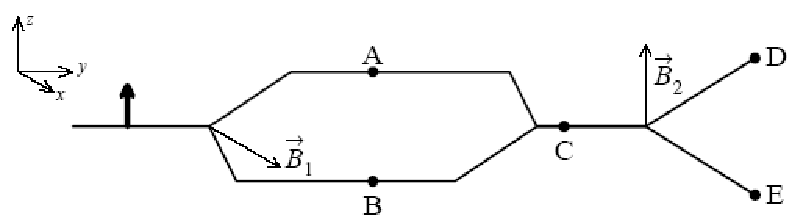
\includegraphics{graphics/SpinREXMQ2005.pdf}
\caption{Mesure du spin 1/2}
\label{fig:MesureSpinEx2011}
\end{figure}

On considérera que le faisceau $A$, tout comme le faisceau $D$ des questions
\ref{Q:q3}. et \ref{Q:q4}. ci-dessous, a la plus grande valeur du spin.

\begin{enumerate}
\item  Donner dans la base $\{\ket{+}_{z},\ket{-}_{z}\}$, la matrice de
l'opérateur $\mathtt{R}_{y}(\theta)$ de rotation d'angle $\theta$ autour de $Oy$
d'un spin $\frac{1}{2}$.

\item Expliquer clairement pourquoi on obtient deux faisceaux à la sortie de
SG1, en donnant l'état du spin en $A$ et $B$ et les probabilités de détection
$\mathcal{P}_{A}$ et $\mathcal{P}_{B}$.

\item\label{Q:q3} On enlève les détecteurs $A$ et $B$ précédents, et les deux
faisceaux sont recombinés en un seul faisceau avant de pénétrer à nouveau dans
un deuxième appareil de Stern-Gerlach, SG2, orienté selon $Oz$. A la sortie de
SG2, on place deux détecteurs $D$ et $E$.

Quel est l'état de spin des quantons détectés en $D$ et $E$ et quelles sont les
probabilités $\mathcal{P}_{D}$ et $\mathcal{P}_{E}$?

\item\label{Q:q4}On place un absorbeur en $A$, c'est-à-dire que SG1 agit comme
un filtre qui ne laisse passer que le faisceau $B$.

Quel est l'état de spin des quantons détectés en $D$ et $E$ et quelles sont les
probabilités $\mathcal{P}_{D}$ et $\mathcal{P}_{E}$? Considérer en particulier
le cas de $\theta=\frac{\pi}{2}$.

\item Quelles commentaires pouvez-vous faire par rapport aux probabilités
obtenues aux questions \ref{Q:q3}. et \ref{Q:q4}.?
\end{enumerate}



\chapter{Postulats et évolution temporelle}
\label{chap:postu}
\minitoc

\bigskip


Nous sommes maintenant suffisamment éclairés sur la \emph{magie} du monde
quantique pour procéder à une généralisation des résultats et principes établis
jusqu'alors à travers les postulats de base de la théorie quantique
(\textbf{section \ref{sec:PostMQ}}). Ces postulats fixent cadre conceptuel
général de la dite théorie. A la \textbf{section \ref{sec:EvolTempo}}, on
s'intéresse à l'évolution temporelle des états quantiques en mettant l'accent
sur les états stationnaires ou états propres de l'énergie. Le chapitre s'achève
avec la \textbf{section \ref{sec:ESpin12}} avec les oscillations de Rabi,
exemples de manipulations des qubits.

\section{Postulats de la théorie quantique}
\label{sec:PostMQ}

\subsection{Postulat 1: Espace des états}

\colorbox[gray]{0.8}{
\parbox[c]{0.9\textwidth}{
\emph{L'état physique d'un système est \textbf{entièrement ou complètement}
défini, à chaque instant, par un élément $\ket{\psi}$ d'un espace de Hilbert
$\mathcal{H}$ approprié.}
}}
\medskip

Toute superposition linéaire d'états
\begin{equation}
\ket{\psi}={\textstyle\sum\limits_n}\ket{\varphi_n}
\langle\varphi_n\ket{\psi} ={\textstyle\sum\limits_n}
\alpha_n\ket{\varphi_n},
\end{equation}
est un élément de $\mathcal{H}$, avec $\alpha_n\in\mathbb{C}$,
$\ket{\varphi_n}\in\mathcal{H}$. Les $\ket{\varphi_n}$ sont donc également
des vecteurs d'état et la base $\{\ket{\varphi_n}\}$ est orthonormée. Ce sont
les amplitudes de projections ou de transition $\alpha_n=\langle
\varphi_n\ket{\psi}$ de l'état $\ket{\psi}$ sur l'ensemble des états
$\ket{\varphi_n} $ du système qui caractérisent l'état du système. Autrement,
$\ket{\psi}$ \emph{\textbf{est l'être mathématique qui décrit la réalité
physique d'un état quantique individuel}}\footnote{On peut aussi dire que c'est
l'être mathématique qui décrit l'information disponible sur un système
quantique.}.

Dans l'expérience de Stern et Gerlach de la \textbf{section \ref{sec:ExpSG}},
$\ket{\psi}=\alpha_{+}\ket{+}+\alpha_{-}\ket{-}$, $\ket{+}$ et $\ket{-}$ étant
les différents états physiques (de spin) des atomes d'argent qui forme le
système quantique.

\subsection{Postulat 2: Amplitudes de probabilité et probabilités}

\colorbox[gray]{0.8}{
\parbox[c]{0.9\textwidth}{
\emph{Si $\ket{\psi}$ et $\ket{\varphi_n} $ représente les états physiques
d'un système quantique, la probabilité $\mathcal{P}(\varphi_n \leftarrow\psi)$
pour l'état $\ket{\psi}$ de passer le test $\ket{\varphi_n}$ est
(\ref{eq:Postu4}), avec $\langle\varphi_n\ket{\psi}$ est l'amplitude de
probabilité ou de transition pour que le système qui était dans l'état
$\ket{\psi}$ se trouve dans l'état $\ket{\varphi_n}$.}
}}
\medskip

Dans l'expérience de Stern et Gerlach, l'amplitude de probabilité de trouver
$\ket{\psi}$ dans l'état $\ket{+}$ est $\alpha_{+}=\langle+\ket{\psi}$,
et la probabilité pour l'état $\ket{\psi}$ de passer donc le test $\ket{+}$ est
$\mathcal{P}(+)  =|\langle+\ket{\psi}|^{2}=|\alpha_{+}|^{2}$.

\subsection{Postulat 3: Grandeurs physiques et opérateurs}

\colorbox[gray]{0.8}{
\parbox[c]{0.9\textwidth}{
\emph{A toute grandeur physique mesurable $\mathcal{A}$ (position, vitesse,
polarisation,etc,) est associé un \textbf{opérateur linéaire hermitien} $A$
agissant dans $\mathcal{H}$: $A$ est le représentant mathématique de cette
grandeur $\mathcal{A}$.}
}}
\medskip

On note que contrairement à la théorie classique, la théorie quantique décrit
de façon fondamentalement différente l'état physique d'un système et les
grandeurs physiques associées. Un état est représenté par un vecteur d'état
normé, une grandeur physique par un opérateur hermitien.

\subsection{Postulat 4: Principe de quantification et de décomposition
spectrale}

\medskip
\colorbox[gray]{0.8}{
\parbox[c]{0.9\textwidth}{
\emph{La mesure d'une grandeur physique $\mathcal{A}$ ne peut donner comme
résultat qu'une des valeurs propres de l'opérateur hermitien $A$
correspondante.}

\emph{Si $\{\ket{\varphi_n}\}$ est la base des \textbf{vecteurs propres} de
$A$,i.e.,}%
\begin{equation}
A\ket{\varphi_n} =a_n\ket{\varphi_n},
\end{equation}
\emph{alors on peut écrire $A$ sous la décomposition spectrale}%
\begin{equation}
A=\sum_n\ket{\varphi_n} a_n\bra{\varphi_n},
\end{equation}
\emph{avec $a_n$ \textbf{une valeur propre} de $A$ ou valeur résultant d'une
mesure idéale faite sur $\mathcal{A}$.}
}}\medskip

\medskip
\colorbox[gray]{0.8}{
\parbox[c]{0.9\textwidth}{
\emph{La probabilité $\mathcal{P}(a_n)$ d'obtenir comme
résultat la valeur propre $a_n$ de l'opérateur hermitien $A$ est}%
\begin{equation}
\mathcal{P}(a_n)=|\langle\varphi_n\ket{\psi}|^{2}=\langle\psi\ket{\varphi_{n
}} \langle\varphi_n\ket{\psi}=|P_n\ket{\psi}|^{2},
\label{eq:Postu4}%
\end{equation}
\emph{où $P_n=\ket{\varphi_n}\bra{\varphi_n}$ est l'opérateur projection
sur la base orthonormée $\{\ket{\varphi_n}\}$.}
}}
\medskip

Ce principe signifie l'ensemble de ces vecteurs propres d'un opérateur hermitien
forme une base complète de l'espace de Hilbert. La description d'un état en
terme d'une grandeur physique $\mathcal{A}$ quantifiée, prenant $N$ valeurs
distinctes $a_n$, repose sur la connaissance de $N$ nombres, avec lesquels on
peut calculer la probabilité d'obtenir la valeur $a_n$. L'ensemble des $a_n$
forme le \textbf{spectre} de $\mathcal{A}$.

Dans l'expérience de Stern et Gerlach, l'opérateur $S$ associé à la grandeur
physique spin $\mathcal{S}$ peut s'écrire%
\begin{equation}
S=\ket{+}\left(+\frac{\hbar}{2}\right)\bra{+}+\ket{-}\left(-\frac{\hbar}{2}
\right)\bra{-}.
\end{equation}
Les vecteurs propres $\ket{+}$ et $\ket{-}$, associés respectivement au valeurs
propres $+\frac{\hbar}{2}$ et $-\frac{\hbar}{2}$ forme une base complète de
l'espace de Hilbert et les $\{+\frac{\hbar}{2},-\frac{\hbar}{2}\}$ forme le
spectre de $S$.

\begin{remark}
\begin{enumerate}
\item Les vecteurs $\ket{\varphi_n} $ et $\ket{\varphi_n^{\prime}}
=e^{i\delta}\ket{\varphi_n}$ représente le même état physique, puisque ce ne
sont que les probabilités d'amplitude qui peuvent être mesurées:%
\begin{equation}
\left\vert \langle\varphi_n^{\prime}\ket{\psi}\right\vert
^{2}=\left\vert \langle\varphi_n\ket{\psi}\right\vert
^{2},~\forall\ket{\psi}\in\mathcal{H}.
\end{equation}
Autrement, il n'est pas possible de distinguer deux états qui diffèrent
seulement par un facteur de phase global $e^{i\delta}$.

\item Cependant, l'état physique $\lambda\ket{\varphi_1}+\mu\ket{\varphi_2}$
est différent de l'état$\lambda\ket{\varphi_1}+\mu\ket{\varphi_2^{\prime}}$.
\end{enumerate}
\end{remark}

\subsection{Postulat 5: Principe de réduction du paquet d'onde}

\colorbox[gray]{0.8}{
\parbox[c]{0.9\textwidth}{
\emph{Si la mesure d'une grandeur physique $\mathcal{A}$ sur le système dans
l'état $\ket{\psi}$ donne le résultat $a_n$, l'état du système immédiatement
après la mesure est}
\begin{equation}
\ket{\varphi_n} =\frac{P_n\ket{\psi}}{\|P_n\ket{\psi}\|}=\frac
{P_n\ket{\psi}}{\sqrt{\bra{\psi}P_n\ket{\psi}}},
\label{eq:PrReduc}
\end{equation}
\emph{la projection normée de $\ket{\psi}$ sur le sous-espace propre associé à
$a_n$. \textbf{Donc la mesure est une projection orthogonale}.}
}}
\medskip

Ce postulat, qui suppose qu'on est dans un cas de mesure QND, est l'énoncé
quantitatif de l'affirmation "\textbf{la mesure perturbe le système}". Si on
effectue une mesure sur le système qui est alors dans l'état propre
$\ket{\varphi_n} $, on trouvera de façon certaine, i.e., avec une probabilité
unité, la valeur propre $a_n$. Ce principe sous-entend que l'appareil de
mesure agit comme un objet classique et ne se préoccupe pas des détails du
processus de la mesure (\emph{point de vue de Copenhagen}).

Dans le cas du spin, si le système $\ket{\psi}$ passe avec succès le test
$\ket{+}$,
\begin{equation}
\frac{P_{+}\ket{\psi}}{\|P_{+}\ket{\psi}\|}=\frac{\ket{+}\langle+\ket{\psi}}
{\sqrt{\langle\psi\ket{+}\langle +\ket{\psi}}}=\ket{+},
\end{equation}
une mesure du spin immédiatement après donnera de façon certaine $+\frac
{\hbar}{2}$: $S\ket{+}=+\frac{\hbar}{2}\ket{+}$.

Soulignons que si $A$ et $B$ commutent, la mesure de $B$ ne fait pas perdre
les informations préalables fournies par une mesure de $A$ (et
réciproquement), mais au contraire les complète; de plus, l'ordre dans lequel
on mesure les deux opérateurs $A$ et $B$ est sans importance. Pour que l'état
du système après la mesure soit déterminé, dans tous les cas, uniquement pour
le résultat obtenu, il faut que cette mesure porte sur un ECOC.

Ajoutons que \emph{si la valeur d'une grandeur physique peut être prédite avec
certitude sans perturber en rien le système, alors il existe une réalité
physique attachée à cette grandeur: }c'est la\textbf{ réalité }EPR
(Einstein-Podolsky-Rosen).


\begin{exercise}
 A system is in the state
\begin{equation}
 \ket{\psi}=\frac{1}{\sqrt{19}}(2\ket{u_1}+2\ket{u_2}+\ket{u_3}+2\ket{u_4}+
\sqrt{6}\ket{u_5})
\end{equation}
where $\{\ket{u_i},\ i=1-5\}$, are a complete and orthonormal set of vectors.
Each $\ket{u_i}$ is an eigenstate of the system’s Hamiltonian corresponding to
the possible measurement result $H\ket{u_i}=i\varepsilon\ket{u_i}$.
\begin{enumerate}
 \item Describe the set of projection operators corresponding to the
possible measurement results.
\item Determine the probability of obtaining each measurement result. What
is the state of the system after measurement if we measure the energy to be
$3\varepsilon$?
\item What is the average energy of the system?
\end{enumerate}
\end{exercise}

\begin{footnotesize}\begin{solution}
\begin{enumerate}
 \item The possible measurement results are $\varepsilon, 2\varepsilon,
3\varepsilon, 4\varepsilon$ and $5\varepsilon$. These measurement results
correspond to the basis states $\ket{u_1},\ket{u_2},\ket{u_3}),\ket{u_4}$, and
$\ket{u_5}$ respectively. Hence the projection operators corresponding to each
measurement result are
\begin{equation}
 P_1=\ket{u_1}\bra{u_1},\; P_2=\ket{u_2}\bra{u_2},\; P_2=\ket{u_3}\bra{u_3},\;
P_4=\ket{u_4}\bra{u_4},\; P_5=\ket{u_5}\bra{u_5}.
\end{equation}
Since the $\ket{u_i}$'s are a set of orthnormal basis vectors, the completeness
relation is satified and
\begin{equation}
\sum_{i}P_i = \mathbb{I}.
\end{equation}
\item We can calculate the probability of obtaining each measurement result
using the \emph{Born rule}. First we need to check and see if the state
is normalized. This is done by calculating $\sum_{i=1}^{5}|c_i|^{2}$ and and
seeing if the result is $1$. We have
\begin{equation}
\begin{split}
 \sum_{i=1}^{5}|c_i|^{2} & =\frac{1}{19}(|2|^2 +|2|^2 +|1|^2 +|2|^2 +|\sqrt{6}|
^2)\\
  & = \frac{1}{19}(4+4+1+4+6)=1.
\end{split}
\end{equation}
The state is normalized, so we can proceed. Before doing so, recall that the
fact that the basis states are orthonormal means that $\bra{u_i}\ket{u_j}
=\delta_{ij}$. So, in the first case, applying the Born rule we have
\begin{subequations}
\begin{align}
 \mathcal{\varepsilon}&=|\bra{u_1}\psi\rangle|^{2}=\langle\psi\ket{u_1}
\bra{u_1}\psi\rangle=\frac{|2|^2}{19}=\frac{4}{19},\\
 \mathcal{\varepsilon}& =|\bra{u_2}\psi\rangle|^{2}=\langle\psi\ket{u_2}
\bra{u_2}\psi\rangle=\frac{|2|^2}{19}=\frac{4}{19},\\
 \mathcal{\varepsilon}&=|\bra{u_3}\psi\rangle|^{2}=\langle\psi\ket{u_3}
 \bra{u_3}\psi\rangle=\frac{|1|^2}{19}=\frac{1}{19},\\
 \mathcal{\varepsilon}&=|\bra{u_4}\psi\rangle|^{2}=\langle\psi\ket{u_4}
 \bra{u_4}\psi\rangle=\frac{|2|^2}{19}=\frac{4}{19},\\
 \mathcal{\varepsilon} &=|\bra{u_5}\psi\rangle|^{2}=\langle\psi\ket{u_5}
 \bra{u_5}\psi\rangle=\frac{|\sqrt{6}|^2}{19}=\frac{6}{19}.
\end{align}
\end{subequations}
If a measurement is made and we find the energy to be $3\varepsilon$, then the
state of the system after measurement is,
\begin{equation}
 \frac{P_3 \ket{\psi}}{\sqrt{\bra{\psi}P_3\ket{\psi}}}
=\frac{\frac{1}{\sqrt{19}}\ket{u_3}}{\sqrt{\frac{1}{19}}}=\ket{u_3}
\end{equation}
\item  The average energy of the system is
\begin{equation}
 \begin{split}
\langle H\rangle & =\sum_{i=1}^{5}E_i \bra{\psi}P_i \ket{\psi}\\
 & =\varepsilon\bra{\psi}P_1 \ket{\psi}+2\varepsilon\bra{\psi}P_2
\ket{\psi}+3\varepsilon\bra{\psi}P_3 \ket{\psi}+4\varepsilon\bra{\psi}P_4
\ket{\psi}+5\varepsilon\bra{\psi}P_5 \ket{\psi}\\
& = \varepsilon\frac{4}{19}+2\varepsilon\frac{4}{19}+3\varepsilon\frac{1}{19}
+4\varepsilon\frac{4}{19}+5\varepsilon\frac{6}{19} = \frac{61}{19}\varepsilon
\end{split}
\end{equation}
\end{enumerate}

\end{solution}
\end{footnotesize}

\section{Évolution temporelle}

\label{sec:EvolTempo}

\subsection{Postulat 6: Évolution temporelle du système}

\colorbox[gray]{0.8}{
\parbox[c]{0.9\textwidth}{
\emph{L'évolution temporelle du vecteur d'état $\ket{\psi(t)}$ est régie par
\textbf{l'équation de Schrödinger ou équation d'évolution}}%
\begin{equation}
i\hbar\frac{d}{dt}\ket{\psi(t)}=H(t)\ket{\psi(t)},
\label{EqSch1}%
\end{equation}
\emph{où $H(t)$ est l'opérateur hermitien associé à l'énergie totale du système
ou \textbf{hamiltonien} du système}.
}}
\medskip

Ce postulat montre que lorsque le système physique est isolé\footnote{Un système
quantique est isolé
\begin{itemize}
\item s'il est dynamiquement indépendant d'un autre système, i.e., s'il n'y a
pas un hamiltonien d'interaction;
\item et s'il est probabilistiquement indépendant (ou séparable) de tout autre
système.
\end{itemize}
}, la théorie quantique est \textbf{déterministe}: elle est capable de prévoir
l'évolution de l'état du système grâce à l'équation de Schrödinger. Pour un état
initial $\ket{\psi(t_0)}$, l'état $\ket{\psi(t)}$ à un instant ultérieur
$t>t_0$ est complètement et uniquement déterminé par l'équation
(\ref{EqSch1}), lorsque $\mathtt{H}$ est connu.

Seulement, lorsqu'une mesure est effectuée, la théorie quantique devient
\textbf{indéterministe}: elle n'est plus capable de prévoir exactement ce qui
va se produire. Elle permet seulement de connaître les probabilités des
différentes occurrences en vertu du postulat de la réduction du paquet d'onde.

La nécessaire \textbf{conservation de la norme du vecteur d'état au cours du
temps} est assurée par l'hermiticité de $\mathtt{H}$. En effet,
\begin{subequations}%
\begin{align}
\frac{d}{dt}\|\ket{\psi(t)}\|^{2}  & =\frac{d}{dt}\langle\psi(t)\ket{\psi(t)}\\
&  =\frac{d\bra{\psi(t)}}{dt}\ket{\psi(t)}+\bra{\psi(t)}
\frac{d\ket{\psi(t)}}{dt}.
\end{align}
\end{subequations}%
Or, en vertu de l'équation (\ref{EqSch1})
\begin{equation}
\left\{
\begin{array}
[c]{c}%
\frac{d\ket{\psi(t)}}{dt}=-\frac{i}{\hbar}H\ket{\psi(t)},\\
\\
\frac{d\bra{\psi(t)}}{dt}=+\frac{i}{\hbar}\bra{\psi(t)}H^{\dag}.
\end{array}
\right.
\label{EqSch2}%
\end{equation}
Par conséquent,%
\begin{equation}
\frac{d}{dt}\|\ket{\psi(t)}\|^{2}=\frac{i}{\hbar}\bra{\psi(t)}H^{\dag}
\ket{\psi(t)}-\frac{i}{\hbar}\bra{\psi(t)}H\ket{\psi(t)}.
\end{equation}
Comme $\mathtt{H}$ est un opérateur hermitien, $H^{\dag}=H$ et
\begin{equation}
\frac{d}{dt}\|\ket{\psi(t)}\|^{2}=0\Rightarrow\langle\psi(t)\ket{\psi(t)}=Cst.
\label{eq:ConsNormV}
\end{equation}

\subsection{Opérateur d'évolution et états stationnaires}

L'équation (\ref{EqSch1}) suggère la correspondance%
\begin{equation}
H\rightarrow i\hbar\frac{d}{dt}.
\end{equation}
qui indique que l'hamiltonien $\mathtt{H}$ est le \textbf{générateur de
l'évolution
temporelle} du système. \textbf{L'opérateur de translation dans le temps} est
donc \begin{equation}
U(t)=e^{-iHt/\hbar},
\end{equation}
Il est unitaire
\begin{equation}
U^{\dagger}(t)=U(-t)=U^{-1}(t),
\label{eq:OpEvol}
\end{equation}

Le vecteur d'état $\ket{\psi(t)}$ au temps $t$ se déduit du vecteur d'état
$\ket{\psi(t_0)}$ au temps $t_0$ de la façon suivante

\colorbox[gray]{0.8}{
\parbox[c]{0.9\textwidth}{
\begin{equation}
\ket{\varphi(t)}=U(t,t_0)\ket{\psi(t_0)}=\exp\left(-i\frac{t-t_0}{h}H\right)
\ket{\psi(t_0)}.
\end{equation}
}}
\medskip

La propriété d'unitarité (\ref{eq:OpEvol}) assure la conservation
(\ref{eq:ConsNormV}) de la norme
\begin{equation}
\langle\varphi(t)\ket{\varphi(t)}=\bra{\varphi(t_0)}U^{\dagger}(t,t_0)U(t,t_
{ 0})\ket{\varphi(t_0)}=\langle\varphi(t_0)\ket{\varphi(t_0)}=1.
\end{equation}

Intéressons nous au cas particulier où $\ket{\varphi}$ est un vecteur propre de
l'énergie du système, i.e.,
\begin{equation}
H\ket{\varphi}=E\ket{\varphi},
\end{equation}

Notons $\{\ket{\varphi_{E}}\}$ ces états propres de l'énergie. Les probabilités
de projection de $|\langle u\ket{\varphi _{E}(t)}|^{2}$ gardent la même valeur
au cours du temps, quel que soit le vecteur de projection $\ket{u}$: elles sont
\textbf{stationnaires.}

\medskip\colorbox[gray]{0.8}{
\parbox[c]{0.9\textwidth}{
\begin{equation}
|\langle u\ket{\varphi_{E}(t)}|^{2}=|\langle u\ket{\varphi_{E}(0)}|^{2}.
\end{equation}
\emph{Ce qui traduit \textbf{l'invariance par translation dans le temps des
états propres de l'énergie}. Autrement dit, l'enveloppe de l'onde ne
change pas au cours du temps, seule sa phase complexe change à vitesse
constante. Cette vitesse dépend de $E$.}
}}
\medskip

Afin de distinguer entre elles les diverses valeurs possibles de l'énergie $E$
et les états propres correspondants, nous leurs affecterons un indice $n$%
\begin{equation}
H\ket{\varphi_n} =E_n\ket{\varphi_n},
\end{equation}
les énergies $E_n$ étant réels.

Pour qu'un état évolue, il doit être une \emph{superposition} d'états
stationnaires,

\medskip
\colorbox[gray]{0.8}{
\parbox[c]{0.9\textwidth}{
\begin{equation}
\ket{\psi(t)}=\alpha_1\ket{\varphi_1}e^{-iE_1t/\hbar}+\alpha_2\ket{
\varphi_2}e^{-iE_2t/\hbar}+\ldots=\sum_n\alpha_n\ket{\varphi_n}
e^{-iE_nt/\hbar},
\end{equation}
ou
\begin{equation}
 \ket{\psi(t)}=\sum_n\alpha_n(t)\ket{\varphi_n},\text{ avec }
\alpha_n(t)=\langle
\varphi_n\ket{\psi(t)}=e^{-i\left(\frac{t-t_0}{\hbar}H\right)}
\alpha_n(t_0).
\end{equation}
}}
\medskip

Ainsi, les termes d'interférence dans $|\langle u\ket{\psi(t)}|^{2}$ dépend du
temps.

L'état stationnaire de plus basse énergie est appelé \textbf{état
fondamental}. A température presque nulle, un système isolé se met dans son
état fondamental. Par exemple, dans les expériences de spectroscopie, grâce à
une force stationnaire qu'on impose au système\footnote{Une onde laser sur une
molécule par exemple.}, on le fait transiter d'un état stationnaire à un autre.


\subsection{Système à deux états}

Représentons un état quelconque d'un quanton comme la superposition des états
de base $\ket{\psi_1}$ et $\ket{\psi_2}$:%
\begin{equation}
\ket{\psi}=\alpha_1\ket{\psi_1}+\alpha_2\ket{\psi_2}.
\end{equation}
Les amplitudes $\alpha_1$ et $\alpha_2$ doivent, en vertu de (\ref{EqSch1}),
satisfaire au système d'équations%
\begin{equation}
\left\{
\begin{array}
[c]{c}%
i\hbar\frac{d}{dt}\alpha_1=h_{11}\alpha_1+h_{12}\alpha_2,\\
\\
i\hbar\frac{d}{dt}\alpha_2=h_{21}\alpha_1+h_{22}\alpha_2.
\end{array}
\right.
\label{eq:SysEqAmpl}%
\end{equation}
Nous devons considérer deux cas.

\subsubsection{Les éléments non-diagonaux $h_{12}$ et $h_{21}$ sont nuls}

La matrice de $\mathtt{H}$ est diagonalisée. Le système d'équations
(\ref{eq:SysEqAmpl})%
\begin{equation}
\left\{
\begin{array}
[c]{c}%
i\hbar\frac{d}{dt}\alpha_1=h_{11}\alpha_1,\\
\\
i\hbar\frac{d}{dt}\alpha_2=h_{22}\alpha_2.
\end{array}
\right.
\end{equation}
Ainsi, si un quanton est, à un instant donné, dans l'état $\ket{\phi_1}$ par
exemple, il ne se trouvera jamais dans l'état $\ket{\psi_2}$. Les états
$\ket{\psi_1} $ et $\ket{\psi_2}$ sont alors des états stationnaires du
quanton, caractérisés par les valeurs $h_{11}$ et $h_{22}$ de l'énergie,%
\begin{equation}
\left\{
\begin{array}
[c]{ccc}%
\alpha_1(t)=\alpha_1(0)e^{-ih_{11}t/\hbar} & \Rightarrow &
|\alpha_1(t)|^{2}=|\alpha_1(0)|^{2}\\
&  & \\
\alpha_2(t)=\alpha_2(0)e^{-ih_{22}t/\hbar} & \Rightarrow &
|\alpha_2(t)|^{2}=|\alpha_2(0)|^{2}%
\end{array}
\right.
\end{equation}
Si à $t=0$, le quanton est dans l'état $\ket{\psi_1} $,
les probabilités de le déceler dans l'un ou l'autre état à instant $t$
ultérieur sont $|\alpha_1(t)|^{2}=1$ et $|\alpha_2(t)|^{2}=0$.

\subsubsection{Les éléments non-diagonaux $h_{12}$ et $h_{21}$ sont non-nuls}

Les deux équations du système (\ref{eq:SysEqAmpl}) sont alors mutuellement
liées. Si à un instant, le quanton se trouve dans l'état $\ket{\phi_1}$, à un
autre instant, il peut se trouver dans l'état $\ket{\psi_2}$.

\medskip
\colorbox[gray]{0.8}{
\parbox[c]{0.9\textwidth}{
\emph{La présence dans la matrice du hamiltonien $\mathtt{H}$ des éléments de
matrice
non-diagonaux non nuls marque la possibilité de \textbf{transitions} du quanton
entre ces deux états de base stationnaires.}
}}


\section{Manipulations de qubits - Oscillations de Rabi}
\label{sec:ESpin12}


Il est légitime de chercher à savoir comment évolue un qubit au cours du temps.
Nous allons rentrer à nouveau au laboratoire pour examiner cela avec un qubit
réaliser grâce au spin $\frac{1}{2}$ que nous plongeons dans un champ magnétique
uniforme $\bls{B}(0,0,B)$.

Nous allons d'abord considérer le phénomène d'un point de vue classique, puis,
à travers la notion de valeur moyenne d'une grandeur physique, nous allons
montrer que les résultats obtenus à partir ces considérations classiques se
retrouvent aisément avec le formalisme quantique.

Il apparaîtra que le moment magnétique d'un quanton plongé dans un tel champ
décrit un mouvement de précession analogue à celui d'une toupie. Ce mouvement de
précession, caractérisé par une pulsation $\omega$, donne lieu à des phénomènes
de résonance, dite \textbf{résonance magnétique}, lorsqu'on module le champ
magnétique $\bls{B}$ en amplitude, à une pulsation $\omega_0$ proche de
$\omega$.

\subsection{Formalisme classique}

En toute rigueur, le formalisme classique est inadapté à l'étude d'un quanton
possédant un spin. Cependant, nous allons voir que les résultats obtenus
illustrent l'allure générale du phénomène mis en jeu, la \textbf{résonance
magnétique}.

En considérant que le moment angulaire de la particule est exclusivement dû au
moment angulaire de spin, une particule placée dans un champ magnétique subit un
moment
\begin{equation}
 \Gamma=\bls{\mu}_{s}\times\bls{B}=\gamma\bls{S}\times\bls{B}=\bls{\omega}
\times\bls{S},
\end{equation}
où $\omega=-\gamma B$  est la \textbf{fréquence de Larmor}. En vertu du théorème
du moment angulaire,
\begin{equation}
	\frac{d\bls{S}}{dt}=\Gamma=\gamma\bls{S}\times\bls{B}.
\end{equation}
Cette équation caractérise le mouvement de précession du spin $\bls{S}$ autour
de l'axe du champ magnétique $\bls{B}$.

En effet, puisque $\bls{B}(0,0,B)$, on a
\begin{subequations}
 \begin{align}
  \frac{dS_{x}}{dt} & =\Gamma_{x}=-\omega S_{y}\label{eq:dSxC}\\
  \frac{dS_{y}}{dt} & =\Gamma_{y}=\omega S_{x}\label{eq:dSyC}\\
  \frac{dS_z}{dt} & =\Gamma_z=0 \label{eq:dSzC}
 \end{align}
\end{subequations}
Par intégration de l'équation (\ref{eq:dSzC}), on trouve sans peine
\begin{equation}
 S_z=Cte,
\end{equation}
qui indique que le mouvement de la particule est rectiligne uniforme le long de
l'axe $Oz$.

Dans le plan $Oxy$, le système d'équations couplées (\ref{eq:dSxC}) et
(\ref{eq:dSyC}) peut s'écrire
\begin{equation}
 \frac{d(S_{x}+iS_{y})}{dt})=i\omega(S_{x}+iS_{y}),
\end{equation}
soit après intégration,
\begin{subequations}
\begin{equation}
 S_{x}(t)+iS_{y}(t)=e^{i(\omega t +\phi)}(S_{x}(0)+iS_{y}(0)),
\end{equation}
ou
\begin{align}
 S_{x}(t) &=\cos(\omega t +\phi)S_{x}(0),\\
 S_{y}(t)&=\sin(\omega t +\phi)S_{y}(0).
\end{align}

\end{subequations}
Dans le plan $Oxy$, la particule effectue un mouvement circulaire à la vitesse
angulaire $\omega$, de phase initiale $\phi$.

On dit que la particule effectue un mouvement de précession à la pulsation
$\omega=-\gamma B$ autour de l'axe $Oz$.

\subsection{Formalisme quantique}

\subsubsection{États stationnaires}

\begin{wrapfigure}{i}{0in}
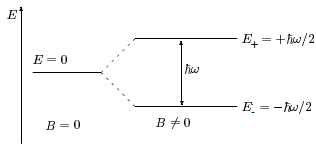
\includegraphics[scale=.9]{graphics/EieSpin.png}
\caption{Séparation du niveau fondamental en deux sous-niveaux en présence du
champ magnétique $\bls{B}$.}
\label{fig:EieSpin}
\end{wrapfigure}
L'hamiltonien qui décrit dans l'espace des états l'évolution du quanton dans
le champ $\bls{B}$ est
\begin{equation}
H=-\gamma BS_z=\omega S_z.
\end{equation}
Il est clair que $[H,S_z]=0$, donc les états propres de $S_z$ sont
des états stationnaires%
\begin{equation}
H\ket{+}=\frac{\hbar\omega}{2}\ket{+},~H\ket{-}=-\frac{\hbar\omega}{2}\ket{-}.
\end{equation}
Le champ magnétique $\bls{B}$ provoque donc l'apparition de deux niveaux
d'énergie séparés par $\hbar\omega$ comme on peut le voir sur la figure
\ref{fig:EieSpin}.

\subsubsection{Rotation et état de spin d'orientation arbitraire}
\label{sec:SpinArbitr1}

\begin{figure}[ptbh]
\begin{minipage}[c]{.45\linewidth}
\centering
  \includegraphics[scale=1]{graphics/SphereBloch.jpg}
\caption{Représentation 3D d'un spin $\frac{1}{2}$ sur une sphère de Bloch:
$\ket{\psi} =e^{-i\varphi/2}\cos\frac{\theta}{2}\ket{+}
+e^{i\varphi/2}\sin\frac{\theta}{2}\ket{-}$, avec $\ket{+}\equiv\ket{0}$,
$\ket{-}\equiv\ket{1}$.}
\label{fig:ReprSpin12Bloch}
\end{minipage} \hfill
\begin{minipage}[c]{.48\linewidth}
\centering
\ifcase\msipdfoutput
  \includegraphics[scale=.7]{graphics/SphereBloch2.png}
\else
  \includegraphics[scale=.7]{graphics/SphereBloch2.pdf}
\fi
\caption{Opérateurs rotations d'un single-qubit.}%
\label{fig:SphereBloch2}%
\end{minipage}

\end{figure}

Afin de fabriquer un qubit dans état de spin d'orientation arbitraire (comme
$\ket{\psi}$ sur la figure \ref{fig:ReprSpin12Bloch}) faisons tourner la
direction du champ magnétique du filtre de Stern et Gerlach et alignons le dans
la direction arbitraire
\begin{equation}
\bls{\hat{u}}(\theta,\varphi)=(\sin\theta\cos\varphi,
\sin\theta\sin\varphi,\cos\theta).
\end{equation}

Ainsi, seule la composante $B_{\bls{u}}=\bls{B}\cdot\bls{\hat{u}}$ du champ
magnétique est non nulle. Avec cette nouvelle orientation, le filtre de Stern et
Gerlach va fabriquer des états $\ket{\pm_{u}}$, obtenus en sélectionnant les
atomes déviés respectivement dans les sens $\pm \bls{\hat{u}}$. Ces états sont
vecteurs propres de l'opérateur%
\begin{equation}
\begin{split}
\sigma_{\bls{u}} & =\bls{\vec{\sigma}}\cdot\bls{\hat{u}}
=\sigma_{x}\sin\theta\cos\varphi+\sigma_{y}\sin\theta\sin\varphi+\sigma_z
\cos\theta\\
& =\begin{pmatrix}
\cos\theta & e^{-i\varphi}\sin\theta\\
e^{i\varphi}\sin\theta & -\cos\theta
\end{pmatrix}.
\end{split}
\end{equation}
Autrement,
\begin{equation}
\ket{+}_{u}=\binom{e^{-i\varphi/2}\cos\frac{\theta}{2}}{e^{i\varphi/2}\sin\frac{
\theta}{2}},\,\ket{-}_{u}=\binom{-e^{-i\varphi/2}\sin\frac{\theta}{2}}{e^{
i\varphi/2}\cos\frac{\theta}{2}}.
\end{equation}

Les états $\ket{+}_{u}$ et $\ket{-}_{u}$ sont les transformés des états par une
rotation qui amène l'axe $Oz$ sur l'axe $\bls{\hat{u}}$. Un choix possible
consiste à faire une première rotation de $\theta$ autour de l'axe $Oy$, suivie
d'une rotation de $\varphi$ autour de l'axe $Oz$.

En effet, sur la sphère de Bloch qu'illustre la figure \ref{fig:SphereBloch2},
les rotations d'angle $\delta$ autour des axes $Ox$, $Oy$ et $Oz$ sont générées,
en vertu de l'équation (\ref{eq:ExpoB}), par les opérateurs,%

\begin{subequations}
\begin{align}
R_{x}(\delta)  &
=e^{-i\frac{\delta}{2}\sigma_{x}}=\mathbb{I}\cos\frac{\delta}{2}
-i\sigma_{x}\sin\frac{\delta}{2}=\begin{pmatrix}
cos\frac{\delta}{2} & -i\sin\frac{\delta}{2}\\
-i\sin\frac{\delta}{2} & \cos\frac{\delta}{2}
\end{pmatrix},\\
R_{y}(\delta)  &
=e^{-i\frac{\delta}{2}\sigma_{y}}=\mathbb{I}\cos\frac{\delta}{2}
-i\sigma_{y}\sin\frac{\delta}{2}=\begin{pmatrix}
\cos\frac{\delta}{2} & -\sin\frac{\delta}{2}\\
\sin\frac{\delta}{2} & \cos\frac{\delta}{2}
\end{pmatrix},\\
R_z(\delta)  &
=e^{-i\frac{\delta}{2}\sigma_z}=\mathbb{I}\cos\frac{\delta}{2}
-i\sigma_z\sin\frac{\delta}{2}=\begin{pmatrix}
e^{-i\frac{\delta}{2}} & 0\\
0 & e^{+i\frac{\delta}{2}}
\end{pmatrix}.
\end{align}%
\end{subequations}%

Pour un axe de rotation quelconque de vecteur unitaire $\bls{\hat{u}}%
=(\bls{\hat{u}}_{x},\bls{\hat{u}}_{y},\bls{\hat{u}}_z)$,
on a%
\begin{equation}
R_{\bls{\hat{u}}}(\delta)=e^{-i\frac{\delta}{2}(\bls{\hat{u}}
\cdot\sigma
)}=\mathbb{I}\cos\frac{\delta}{2}-(\bls{\hat{u}}\cdot\sigma)i\sin\frac
{\delta}{2},
\end{equation}
où
$\bls{\hat{u}}\cdot\sigma=u_{x}\sigma_{x}+u_{y}\sigma_{y}+u_z\sigma_z
$.

Les matrices de Pauli étant hermitiennes, les opérateurs de rotation
$R_{\bls{\hat{u}}}(\delta)$ sont unitaires:
\begin{equation}
R_{\bls{\hat{u}}}^{\dagger}(\delta)=R_{\bls{\hat{u}}}(-\delta
)=R_{\bls{\hat{u}}}^{-1}(\delta).
\end{equation}

Dans la base standard $\{\ket{+},\ket{-}\}$, la matrice générale de rotation du
spin $\frac{1}{2}$ d'une rotation de $\theta$ autour de l'axe $Oy$ suivie d'une
rotation de $\varphi$ autour de l'axe $Oz$ est alors
\begin{equation}
\mathcal{D}^{1/2}(\theta,\varphi)=e^{-i\frac{\varphi}{2}\sigma_z}e^{-i\frac{
\theta}{2}\sigma_{y}}=\begin{pmatrix}
e^{-i\varphi/2}\cos\frac{\theta}{2} & -e^{-i\varphi/2}\sin\frac{\theta}{2}\\
e^{i\varphi/2}\sin\frac{\theta}{2} &
e^{i\varphi/2}\cos\frac{\theta}{2}
\end{pmatrix}.
\end{equation}

\medskip\colorbox[gray]{0.8}{
\parbox[c]{0.9\textwidth}{
\emph{Le fait le plus remarquable à propos dans l'expression de
$\mathcal{D}^{1/2}(\theta,\varphi)$ est qu'elle est multivoque: la
représentation d'une rotation de $\theta\ =2\pi$ est la matrice $-\mathbb{I}$,
alors que la rotation équivalente de $\theta\ =0$ ou $\theta\ =4\pi$ donne
$\mathbb{I}$. C'est une caractéristique des représentations de spin
demi-entier.}
}}
\medskip

L'ensemble des matrices $\mathcal{D}^{1/2}(\theta,\varphi)$ forme \textbf{le
groupe} $SU(2):$

\begin{itemize}
\item $S$: Spécial, i.e., $\det\mathcal{D}^{1/2}=+1$;

\item $U$: Unitaire, i.e.,
$(\mathcal{D}^{1/2})^{\dagger}=[\mathcal{D}^{1/2}]^{-1}$;

\item $2$: matrice $2\times2$.
\end{itemize}

\subsubsection{Évolution du qubit}

Supposons maintenant qu'à l'instant $t=0$, le quanton soit dans l'état propre
$\ket{+}_{u}$ de $S_{u}$,%
\begin{equation}
\ket{\psi(0)}=\ket{+}_{u}=e^{-i\varphi/2}\cos\frac{\theta}{2}\ket{+}
+e^{i\varphi/2}\sin\frac{\theta}{2}\ket{-}.
\end{equation}
qui n'est visiblement pas un état stationnaire. A un instant $t>0$, le quanton
est, d'après le \emph{postulat d'évolution}, dans l'état,
\begin{equation}%
\label{SpinT}%
\begin{split}
\ket{\psi(t)}&  =e^{-iHt/\hbar}\ket{\psi(0)}=e^{-i\omega t/2}e^{-i\varphi/2}\cos
\frac{\theta}{2}\ket{+}+e^{+i\omega t/2}e^{i\varphi/2}\sin\frac{\theta}{2}
\ket{-}\\
&  =e^{-i(\varphi+\omega t) /2}\cos\frac{\theta}{2}\ket{+} +e^{i(\varphi+\omega
t) /2}\sin\frac{\theta}{2}\ket{-}.
\end{split}
\end{equation}%
Il apparaît que si à $t=0$ le spin est orienté suivant la direction
$\bls{u}_0(\theta,\varphi)$, à l'instant $t$, il est orienté dans la
direction $\bls{u} _{t}(\theta,\varphi+\omega t)$. Au cours du temps, la
direction du spin tourne, dans le sens trigonométrique, autour de l'axe de
quantification $Oz$ à la vitesse angulaire $\omega=-\gamma B$, proportionnelle
au champ magnétique. Ce mouvement qui coïncide avec le mouvement du moment
magnétique classique porte le nom de \textbf{précession de Larmor}. On remarque
que c'est après $t_{etat}=\frac{4\pi}{\omega}$ que le quanton retrouve son état
initial.

D'après (\ref{SpinT}) lors d'une mesure de $\mathcal{S}_z$ à l'instant $t$
on obtient

\begin{enumerate}
\item $+\frac{\hbar}{2}$ avec une probabilité $|\langle +\ket{\psi(t)}|^{2}
=\cos^{2}\frac{\theta}{2}$;

\item $+\frac{\hbar}{2}$ avec une probabilité $|\langle -\ket{\psi(t)}|^{2}
=\sin^{2}\frac{\theta}{2}$.
\end{enumerate}

Ces probabilités sont bien évidemment indépendantes du temps puisque
$\ket{+}$ et $\ket{-}$ sont des états stationnaires.

La probabilité pour que, à l'instant $t$, le système retrouve son état de spin
initial $\ket{\psi(0)}\equiv\ket{+}_{u}$ est
\begin{equation}
\begin{split}
\mathcal{P}_{+}(t)&  =|_{u}\bra{+}\psi(t)\rangle|^{2}=|e^{-i\omega
t/2}\cos^{2}\frac{\theta}{2}+e^{+i\omega t/2}\sin^{2}\frac{\theta}{2}|^{2}\\
&  =\cos^{4}\frac{\theta}{2}+\sin^{4}\frac{\theta}{2}+\frac{1}{2}\cos^{2}%
\frac{\theta}{2}\sin^{2}\frac{\theta}{2}\cos\omega t.
\end{split}
\end{equation}
\emph{Les probabilités oscillent à une fréquence proportionnelle à la
fréquence de Larmor} $\omega=\frac{E_{+}-E_{-}}{\hbar}=\frac{\Delta E}{\hbar}$.
$\Delta E$ est la dispersion sur l'énergie: le quanton passe d'un niveau à
l'autre avec un temps caractéristique $\Delta t\simeq\frac{\hbar}{2\Delta E}$.

Si $\ket{+}_{u}\equiv\ket{+}_{x}$, alors $\theta=\frac{\pi}{2}$ et $\varphi=0$
et cette probabilité devient%
\begin{equation}
\mathcal{P}_{+}(t)=|_{x}\bra{+} \psi(t)\rangle|^{2}
=|\frac{1}{2}\left(e^{-i\omega t/2}+e^{+i\omega t/2}\right)|^{2}
=\cos^{2}\left( \frac{\omega t}{2}\right).
\end{equation}


Afin de comprendre cette précession du spin ou les oscillations des
probabilités, déterminons les valeurs moyennes des trois composantes du spin
$\frac{1}{2}$ dans l'état $\ket{\psi(t)}$:%
\begin{equation}
\bra{\psi(t)}S_z\ket{\psi(t)}=
\left(\frac{\hbar}{2}\right)\cos^{2}\frac{\theta}{2}+\left(-\frac{\hbar}{2}
\right)\sin^{2}\frac{\theta}{2}=\frac{\hbar}{2} \cos\theta.
\end{equation}
Cette valeur moyenne est sans surprise indépendante du temps puisque
$[H,S_z]=0$. En utilisant les expressions matricielles de $S_{x}$ et $S_{y}$,
on trouve sans difficulté
\begin{subequations}%
\label{MoySxSy}%
\begin{align}
\bra{\psi(t)} S_{x}\ket{\psi(t)} &
=\hbar\cos\frac{\theta}{2}\sin\frac{\theta}{2}\cos(\varphi+\omega t)
=\frac{\hbar}{2}\sin\theta\cos\left(\varphi+\omega t\right),\\
\bra{\psi(t)} S_{y}\ket{\psi(t)} &
=\hbar\cos\frac{\theta}{2}\sin\frac{\theta}{2}\sin(\varphi+\omega t)
=\frac{\hbar}{2}\sin\theta\sin\left(\varphi+\omega t\right).
\end{align}%
\end{subequations}%
$S_{x}$ et $S_{y}$ ne sont visiblement pas des constantes de mouvement. Les
équations (\ref{MoySxSy}) peuvent encore s'écrire%
\begin{equation}
\bra{\psi(t)} S_{x}+iS_{y}\ket{\psi(t)} =\frac{\hbar}{2}\sin\theta e^{i(\varphi
+\omega t)}=e^{i\omega t}(\bra{\psi(0)}S_{x}+iS_{y}\ket{\psi(0)}),
\end{equation}
montrant que $\langle \bls{S}(t)\rangle$ précesse autour de $Oz$ à la
fréquence $\omega$:%
\begin{equation}
\frac{d\left\langle \bls{S}\right\rangle }{dt}=\bls{\omega
}\wedge\left\langle \bls{S}\right\rangle.
\end{equation}
Après $t_{prec}=\frac{2\pi}{\omega},$ le quanton retrouve sa direction initiale.

A travers la valeur moyenne du spin, on retrouve le même comportement que le
moment magnétique classique.

Cette propriété, la précession, est à la base des techniques de
\textbf{résonance magnétique.}

\newpage


\section{Exercices et problèmes}

\subsection{Moment magnétique du deutéron}

Un noyau de deutérium plongé dans un champ magnétique $\bls{B}$ possède
trois états $\ket{+}$, $\ket{0} $, $\ket{-}$ d'énergie $+E_0$, $0$, $-E_0$
respectivement, avec $E_0=\hbar\omega$. Ce noyau a un moment magnétique et on
suppose que l'opérateur $M$ associé à la projection de ce moment sur une
direction fixe perpendiculaire au champ $\bls{B}$ a la forme
$M=\mu_0A,$ avec $\mu_0>0$ et $A$ défini par%
\begin{equation}
A\ket{+}=\frac{1}{\sqrt{2}}\ket{0},\,A\ket{0}=\frac{1}{\sqrt{2}}(\ket{+}+\ket{-}
),\,A\ket{-} =\frac{1}{\sqrt{2}}\ket{0} .
\end{equation}

\begin{enumerate}
\item Écrire la matrice représentant $A$ dans la base $\{\ket{+},\ket{0},\ket{-}
\}$. $A$ est-il hermitien?

\item Calculer les valeurs propres $m_1$, $m_2$ et $m_3$ de $M$ (avec
$m_1>m_2>m_3$) et déterminer les vecteurs propres normalisés correspondant 
$\ket{m_1}$, $\ket{m_2}$, $\ket{m_3}$.

\item On suppose qu'à l'instant $t=0$, le noyau est dans l'état
$\ket{\psi(0)}=\ket{m_1}$. Calculer $\ket{E}$ et $\Delta E$ dans cet état.

\item Calculer $\av{M}$ dans l'état $\ket{\psi(t)}$ en fonction de $\omega$.

\item Quelles sont, en fonction de $\omega$, les probabilités de trouver
$m_1$, $m_2$ et $m_3$ lors d'une mesure de $M$ sur l'état $\ket{\psi(t)}$?

\item Interpréter physiquement l'évolution de la composante transverse du
moment magnétique.
\end{enumerate}

\subsection{Précession de Larmor}

On considère un quanton de spin $\frac{1}{2}$ dont les états propres de
$S_z$ sont notés $\ket{+}_z$ et $\ket{-}_z$. On considère un état de spin
quelconque $\ket{\psi}$ caractérisé par les amplitudes de transition
$\alpha=_z\langle+\ket{\psi}$ et $\beta=_z\langle-\ket{\psi}$.

\begin{enumerate}
\item Quelle sont les probabilités des transitions $\ket{+}_z\longleftarrow
\ket{\psi}$ et $\ket{-}_z\longleftarrow\ket{\psi}$? Quelle relation doit lier
ces deux quantités?

\item On suppose que le quanton possède un moment magnétique $\bls{\mu
}$ et qu'il est placé dans un champ magnétique $\bls{B}=(0,0,B)$. Le
hamiltonien étant $H=-\bls{\mu}\cdot\bls{B}=\omega S_z$ avec
$\omega=-\gamma B$, quels sont les états stationnaires de ce quanton? Préciser
les énergies associées à ces états.

\item Si à l'instant $t=0$ le quanton est dans un état de spin qui soit état
propre d'une composante de $\bls{S}$ orthogonale à $\bls{B}$,
par exemple $S_{x}$. Notons $\ket{+}_{x}$ cet état.

\begin{enumerate}
\item Cet état est-il stationnaire?

\item Quelle est à l'instant $t>0$ et dans la base $\{\ket{+}_z,\ket{-}_z
\}$, l'amplitude de probabilité $_{x}\langle+\ket{\varphi(t)}$ si
$\varphi(0)=\ket{+}_{x}$?

\item Quelle est la probabilité $\mathcal{P}_{+}(t)=|_{x}\langle
+\ket{\varphi(t)}|^{2}$ pour que, à l'instant $t>0$, le quanton se retrouve dans
son état initial $\ket{+}_{x}$? Même question pour $\mathcal{P}_{-}(t)=
|_{x}\langle -\ket{\varphi(t)}|^{2}$.
\end{enumerate}

\item Les variations temporelles de ces probabilités sont le plus souvent
interprétées par référence à l'évolution des valeurs moyennes des composantes
du spin. Calculer ces valeurs moyennes dans l'état $\ket{\varphi(t)}$ et
conclure.

\item Le quanton est un neutron de longueur d'onde
$\lambda=1.55\opn{\mathring{A}}$ et masse $mc^{2}=939.566\opn{MeV}$.
On rappelle que $\hbar c=1\,973\opn{eV\mathring{A}}$.

\begin{enumerate}
\item Calculer la vitesse du neutron.

\item Déduire de la figure (\ref{fig:PrecLarmor}) la valeur de la vitesse
angulaire de précession du spin.

\item Le champ magnétique vaut $B=15.5\times10^{-4}\opn{T}$. En déduire
la valeur du moment magnétique du neutron.
\end{enumerate}
\end{enumerate}

\begin{figure}[ptbh]
\centering
\ifcase\msipdfoutput
	\includegraphics{graphics/PrecLarmor.eps}
\else
	\includegraphics{graphics/PrecLarmor.pdf}
\fi
\caption{Précession de Larmor des neutrons. Variation de $\langle
S_{x}\rangle _{\ket{\psi(t)}}$ en fonction de la
distance (c'est-à-dire du temps de parcours).}%
\label{fig:PrecLarmor}%
\end{figure}

\subsection{Détection des électrons}

Des électrons polarisés, avec des spins $\frac{1}{2}$ polarisés ($+$) dans la
direction $Oz$ pénètrent dans une région où règne un champ magnétique statique
$\bls{B}=(B_0,0,0)$. Les électrons se déplacent dans la direction $Oy$.
Après un temps $T$, les électrons atteignent un appareil de Stern-Gerlach où le
gradient de champ est orienté suivant $Oz$.

\begin{enumerate}
\item Écrire, dans la base qui diagonalise la matrice de Pauli $\sigma_z$, la
matrice du hamiltonien d'interaction $H_0$ dans la région où règne le champ
$\bls{B}=(B_0,0,0)$. On posera $\omega _0=-\gamma B_0$.

\item \label{q:ExoSpinDetec2}Sur un détecteur $D$ placé après l'appareil de
Stern-Gerlach, on ne peut détecter que les électrons de spin ($-$) dans la
direction $Oz$. Trouver les valeurs de $B_0$ qui permettent à tous les
électrons d'atteindre le détecteur $D$.

\item Pour la valeur minimale de $B_0$, de la question \ref{q:ExoSpinDetec2}, 
quel est le pourcentage des électrons qui atteignent $D$ si le temps de parcours 
dans la région où règne $B_0$ est $\frac{T}{2}$ et non $T$?
\end{enumerate}


\subsection{Réalisation expérimentale d'une porte logique 1-qubit}

On rappelle que le spin de l'électron \emph{génère} un moment magnétique
$\bls{\mu}=\gamma\bls{S}$, où $\gamma=g\frac{q}{2m}$ est le \emph{rapport
gyromagnétique} et $g$ est le \emph{facteur de Landé}.

L'hamiltonien qui décrit dans l'espace des états l'évolution de l'électron dans
le champ $\bls{B}=(0,0,B_0)$ est $\mathtt{H}=-\bls{\mu}\cdot\bls{B}$. On posera
$\omega_0=\gamma B_0$, la pulsation de Larmor ou pulsation de résonance.

On rappelle que l'opérateur de rotation autour de $Ou$ est
\begin{equation}
\mathtt{R}_u(\theta)= e^{-i\theta\sigma_{u}/2} =(\cos\frac{\theta}{2})\mathbb{I}
-i(\sin\frac{\theta}{2})\sigma_{u}.
\end{equation}
\begin{enumerate}
\item Donner, dans la base qui diagonalise $\mathtt{S}_z$, l'expression de la
matrice de $\mathtt{H}$ en fonction de $\omega_0$. Quels sont les niveaux
d'énergie du système?

\item Le vecteur d'état du spin, $\ket{\psi(t)}$ se décompose dans la base des
états propres de $\mathtt{S}_z$ sous la forme
\begin{equation}
\ket{\psi(t)} =\alpha_0(t)\ket{0}+\alpha_1(t)\ket{1}.
\end{equation}

\begin{enumerate}
\item En résolvant matriciellement l'équation de Schrödinger,
$i\hbar\frac{d}{dt}\ket{\psi(t)} =\mathtt{H}(t)\ket{\psi(t)}$, donner les
expressions de $\alpha_{0,1}(t)$, en fonction de $\alpha_{0,1}(0)$ et
$\mathtt{R}_z(\theta)$. On précisera l'expression de $\theta$.

\item Combien de temps faut-il laisser agir le champ magnétique statique
$\bls{B}_0$ sur le spin de l'électron pour réaliser, à un facteur de phase
globale près sur $\alpha_{0,1}(t)$, une porte q-logique $\mathtt{Z}$,
$\ket{k}\Qcircuit @C=1em @R=.7em { & \gate{\mathtt{Z}} & \qw}(-1)^{k}\ket{k}$?
Pourquoi ce facteur de phase globale est-il non-significatif du point de vue de
la mesure?
\end{enumerate}

\item Afin de réaliser une porte q-logique $\mathtt{X}$, $\ket{k}\Qcircuit
@C=1em @R=.7em {& \gate{\mathtt{X}} & \qw}\ket{1-k}$, on ajoute au champ
statique $\bls{B}_0$ un champ $\bls{B}_1(t)$ situé dans le plan $xOy$ tournant
dans le sens trigonométrique avec la vitesse angulaire $\omega$,
\begin{equation}
\bls{B}_1(t)=B_1(\bls{e}_{x}\cos\omega t+\bls{e}_{y}\sin\omega t) .
\end{equation}
On posera $\omega_1=\gamma B_1$ la \emph{fréquence ou pulsation de Rabi} et
$\delta=\omega+\omega_0$ \emph{le désaccord à la résonance}.

\begin{enumerate}
\item Écrire la nouvelle matrice du hamiltonien $\mathtt{H}(t)$ du système dans
la base où $\mathtt{S}_z$ est diagonale, puis le système d'équations
différentielles auquel obéissent $\alpha_{0,1}(t)$.

\item Pour résoudre ce système, on se place dans le référentiel tournant avec le
champ en posant
\begin{equation}
\alpha_0(t)=\beta_0(t)e^{-i\omega t/2},\,\alpha_1(t)=\beta_1(t)e^{+i\omega
t/2},\,\ket{\tilde{\psi}(t)}=\beta_0(t)\ket{0}+\beta_1(t)\ket{1}.
\end{equation}

\begin{enumerate}
\item Écrire $\ket{\tilde{\psi}(t)}$ en fonction de l'opérateur rotation
$\mathtt{R}_z$ et $\ket{\psi(t)}$ afin de justifier l'expression
\emph{référentiel tournant}.
\item Montrer que
\begin{equation}
i\hbar\begin{pmatrix}\dot{\beta}_0(t)\\\dot{\beta}_1(t)\end{pmatrix}
=\tilde{\mathtt{H}}\begin{pmatrix}\beta_0(t)\\\beta_1(t)\end{pmatrix},
\end{equation}
où $\tilde{\mathtt{H}}$ est fonction des matrices de Pauli et indépendant du
temps.

\item A partir de $\ket{\tilde{\psi}(t)}=\tilde{\mathtt{U}}(t)
\ket{\tilde{\psi}(0)}$, déduire la relation entre $\alpha_{0,1}(t)$ et
$\alpha_{0,1}(0)$ en fonction des matrices de Pauli.
\end{enumerate}
\end{enumerate}

\item Lorsque $\delta=0$, combien de temps faut-il laisser agir le champ
tournant pour réaliser, à un facteur de phase globale près, une porte qu-logique
$\mathtt{X}$?

\item A l'instant $t=0$, le spin est dans l'état pur $\ket{0}$.

\begin{enumerate}
\item Quelle est la probabilité $\mathcal{P}_{1\leftarrow0}(t)$ de trouver au
temps $t$ le spin dans l'état $\ket{1}$?

\item À quel instant cette probabilité est-elle maximale? Montrer que la porte
q-logique $\mathtt{X}$ consiste à faire basculer le spin de l'état $\ket{0}$ à
$\ket{1}$ et vice-versa. Quel est l'équivalent \emph{classique} de cette
opération logique quantique?
\end{enumerate}
\end{enumerate}

\subsection{QuTiP - Evolution d'un état de spin 1/2}

Écrire un programme (script) en Python utilisant QuTiP pour répondre aux 
questions suivantes.

L'évolution d'un quanton de spin 1/2, de moment magnétique $\mathbf{\mu}$, dans un champ magnétique $\textbf{B}(0,0,B)$, peut être décrit par l'hamiltonien $H=-\mathbf{\mu}.\textbf{B}=\omega S_z$. Le quanton pénètre dans le champ magnétique dans l'état $\ket{+}_x$. On prendra : $\hbar\omega=0.5$.
\begin{enumerate}
\item Définir l'hamiltonien $H$, ainsi que ses états propres $\ket{+}_z$ et $\ket{-}_z$.
\item Exprimer les états $\ket{+}_x$ et $\ket{-}_x$ en fonction des états propres du hamiltonien $H$.
\item Définir les projecteurs $P_+$ et $P_-$ respectivement sur les états $\ket{+}_x$ et $\ket{-}_x$
\item Le quanton initialement dans l'état $\ket{+}_x$ pénètre dans le champ magnétique à $t=0$. Résoudre l'équation de schr\"odonger, pour $t\in[0,30]$. Calculer en même temps les valeurs moyennes de $P_+$, $P_-$, $H$ et $H^2$.

\textbf{Note} : la valeur moyenne $\bra{\psi(t)}P_+\ket{\psi(t)}=\bra{\psi(t)}+\rangle_x ._x\langle+\ket{\psi(t)}=\mathcal{P}_+(t)$, est la probabilité de trouver le quanton à l'instant $t$ dans l'état $\ket{+}_x$. De même pour $P_-$.
\item Représenter, pour $t\in[0,30]$, les probabilités de trouver le quanton dans l'état $\ket{+}_x$ et $\ket{-}_x$. Que remarque-t-on?
\item Calculer pour $t=30s$ la déviation standard de $\Delta H$.
\end{enumerate}



\chapter{Corrélations quantiques}

\minitoc

\bigskip

Nos incursions dans le monde quantique ce sont jusqu'à présent limités aux états
à un quanton. L'objet de ce chapitre est la description d'états à deux quantons
qui conduisent à des configurations très riches dites \textbf{intriquées} ou
\textbf{corrélées}. Ces corrélations sont à la base du calcul quantique. Une
fois assimilé le cas à deux quantons, la généralisation à un nombre quelconque
de quantons est facile.

Dans la vie courante, on a par exemple des \emph{corrélations par échange du
signal} tel que le feu rouge correspond à l'arrêt des véhicules et au passage
des piétons. Mais on a pas de corrélation entre particules classiques.

Le chapitre commence avec la \textbf{section \ref{sec:ProdTen}} qui introduit
les notions de produit tensoriel et d'états intriqués indispensables à la
description des états à plusieurs quantons. La \textbf{section \ref{sec:Bell}}
est consacrée à l'étude des importantes conséquences physiques telles les
inégalités de Bell et les interférences des états corrélés, qui permettent de
mettre en exergue le caractère non local et non séparable de la théorie
quantique. En effet, il apparaît que
\begin{enumerate}
\item les corrélations quantiques ne disparaissent pas lorsqu'on augmente la
distance entre les quantons, et leur origine ne peut être la réception d'un
signal commun;

\item les corrélations quantiques violent les inégalités de Bell et donc leur
origine ne peut non plus être une décision commune prise à la source.
\end{enumerate}

La dernière section, \textbf{section \ref{sec:IQ}}, est réservée aux
applications en information quantique comme la cryptographie et la téléportation
quantique.

\section{Produit tensoriel et états intriqués}
\label{sec:ProdTen}

\subsection{États}

Soient deux systèmes physiques isolés $(S_{1})$ et $(S_{2})$, d'espaces d'états
correspondants respectifs $\mathcal{H}_{1}$ et $\mathcal{H}_{2}$. Si on
considère l'ensemble de ces deux états comme un système unique $(S)$, quel est
l'espace des états $\mathcal{H}$ associé?

\colorbox[gray]{0.8}{
\parbox[c]{0.9\textwidth}{
\begin{definition}
Par définition, l'espace d'états $\mathcal{H}$ est appelé \textbf{produit
tensoriel} de $\mathcal{H}_{1}$ et $\mathcal{H}_{2}$, et noté $\mathcal{H}%
=\mathcal{H}_{1}\otimes\mathcal{H}_{2}$, si à tout couple de vecteurs,
$(\ket{\psi_{1}},\ket{\psi_{2}})\in\mathcal{H}_{1}\times\mathcal{H}_{2}$, on
associe un vecteur de $\mathcal{H}$, noté $\ket{\psi_{1}}\otimes\ket{\psi_{2}}$
et appelé produit tensoriel de $\ket{\psi_{1}}$ et $\ket{\psi_{2}}$, tel que
cette correspondance soit linéaire par rapport à la multiplication par des
scalaires, et distributive par rapport à l'addition vectorielle:
\begin{subequations}%
\begin{align}
[\ket{\psi_{1}}+\lambda\ket{\psi_{1}^{\prime}}]\otimes\ket{\psi_{2}} &
=\ket{\psi_{1}}\otimes\ket{\psi_{2}}+\lambda\ket{\psi_{1}^{\prime}}\otimes
\ket{\psi_{2}},\\
\ket{\psi_{1}}\otimes[\ket{\psi_{2}}+\lambda\ket{\psi_{2}^{\prime}}]   &
=\ket{\psi_{1}}\otimes\ket{\psi_{2}}+\lambda\ket{\psi_{1}}\otimes\ket{\psi_{2}^{
\prime}},
\end{align}
\end{subequations}%
et tel que si $\{\ket{\psi_{1}^{i}}\}$ et $\{\ket{\psi_{2}^{j}}\}$ sont
respectivement des bases de $\mathcal{H}_{1}$ et $\mathcal{H}_{2}$, alors
$\{\ket{\psi_{1}^{i}}\otimes\ket{\psi_{2}^{j}}\}$ est une base de
$\mathcal{H}$.
\end{definition}
}}
\medskip

Pour des raisons de simplicité, on note le plus souvent
\begin{equation}
\ket{\psi_{1}}\otimes\ket{\psi_{2}}=\ket{\psi_{1}}\ket{\psi_{2}}
=\ket{\psi_{1}\psi_{2}}.
\end{equation}

\colorbox[gray]{0.8}{
\parbox[c]{0.9\textwidth}{
\begin{definition}
Le \textbf{produit scalaire} sur $\mathcal{H}=\mathcal{H}_{1}\otimes
\mathcal{H}_{2}$ se définit de la manière suivante%
\begin{equation}
\langle\psi_{1}^{\prime}\psi_{2}^{\prime}\ket{\psi_{1}\psi_{2}}=
\langle\psi_{1}^{\prime}\ket{\psi_{1}}
\langle\psi_{2}^{\prime}\ket{\psi_{2}}.
\end{equation}
\end{definition}
}}
\medskip

Si $\{\ket{n}\}$ est une base orthonormée de $\mathcal{H}_{1}$ et $\{\ket{m}\}$
une base orthonormée de $\mathcal{H}_{2}$ telles que%
\begin{equation}
\ket{\psi_{1}}=\sum_{n=1}^{N}\alpha_{n}\ket{n},\ \ket{\psi_{2}}=\sum_{m=1}^{M}
\alpha_{m}\ket{m},
\end{equation}
alors%
\begin{equation}
\ket{\psi_{1}\psi_{2}}=\sum_{n,m}\alpha_{n}\alpha_{m}\ket{nm},
\label{eq:PT2}%
\end{equation}
avec%
\begin{equation}
\langle n^{\prime}m^{\prime}\ket{nm}=\delta_{n^{\prime}n}\delta_{m^{\prime}m}.
\end{equation}

\begin{example}
On considère dans la base $\{\ket{0},\ket{1}\}$ les vecteurs d'état
$\ket{\psi_1}=\frac{1}{\sqrt{2}}(\ket{0}-\ket{1})=
\frac{1}{\sqrt{2}}\binom{1}{-1}$ et
$\ket{\psi_{2}}=\frac{1}{\sqrt{2}}(\ket{0}+\ket{1})=\frac{1}{\sqrt{2}}
\binom{1}{1}$. Dans la base $\{\ket{00},\ket{01},\ket{10},\ket{11}\}$ le produit
tensoriel $\ket{\psi_{1}}\otimes\ket{\psi_{2}}$ a pour matrice%
\begin{equation}
\ket{\psi_{1}}\otimes\ket{\psi_{2}}=\frac{1}{\sqrt{2}}\binom{1.\ket{\psi_{2}}}{
-1.\ket{\psi_{2}}}=\frac{1}{2}\begin{pmatrix}
1\\
1\\
-1\\
-1
\end{pmatrix}.
\end{equation}

\end{example}

On peut considérer qu'un état produit $\ket{\psi_{1}} \otimes\ket{\psi_{2}}$
représente la simple juxtaposition de deux systèmes, l'un dans l'état
$\ket{\psi_{1}}$ et l'autre dans l'état $\ket{\psi_{2}}$. On dit encore que,
dans un tel état, les deux systèmes sont \textbf{sans corrélations}: les
résultats de deux types de mesures pourtant soit sur un système, soit sur
l'autre, correspondent à des variables aléatoires indépendantes. Une telle
situation est réalisée lorsque les deux systèmes ont été préparés indépendamment
et séparément dans les états $\ket{\psi_{1}}$ et $\ket{\psi_{2}}$ et qu'on les
réunit ensuite, sans qu'ils interagissent.

\subsection{Opérateurs}

Soient $A$ et $B$ deux opérateurs agissant respectivement dans $\mathcal{H}_{1}$
et $\mathcal{H}_{2}$. On peut construire un opérateur $A\otimes B$ agissant dans
$\mathcal{H}=\mathcal{H}_{1}\otimes\mathcal{H}_{2}$ tel que%
\begin{equation}
(A\otimes B)\ket{\psi_{1}\psi_{2}}=A\ket{\psi_{1}}\otimes B\ket{\psi_{2}}.
\end{equation}
Si $A$ et $B$ sont des opérateurs hermitiens, alors $A\otimes B$ est un
opérateur hermitien.

Une classe simple des opérateurs de $\mathcal{H}$ est
\begin{equation}
A\otimes\mathbb{I}_{B}\text{ et }\mathbb{I}_{A}\otimes B.
\end{equation}
Il est à noter que
\begin{equation}
(A\otimes B)\cdot(C\otimes D)=(AC)\otimes(BD).
\end{equation}
Ainsi%
\begin{equation}
[A\otimes\mathbb{I}_{B},\mathbb{I}_{A}\otimes B]=(A\otimes\mathbb{I}_{B})\cdot
(\mathbb{I}_{A}\otimes B)-(\mathbb{I}_{A}\otimes B)\cdot(A\otimes\mathbb{I}_{B})
=0.
\end{equation}

Si $\ket{\psi_{1}}$ est un vecteur propre de l'opérateur $A$ avec la valeur
propre $a$, $A\ket{\psi_{1}}=a\ket{\psi_{1}}$, alors $\ket{\psi_{1}\otimes
\psi_{2}}$ est aussi vecteur propre de $A\otimes\mathbb{I}_{B}$ avec la valeur
propre $a$:%
\begin{equation}
A\otimes\mathbb{I}_{B}\ket{\psi_{1}\otimes\psi_{2}}=a\ket{\psi_{1}\otimes\psi_{2
}}.
\end{equation}
On omet très souvent d'écrire explicitement les opérateurs identités
$\mathbb{I}_{A}$ et $\mathbb{I}_{B}$ pour écrire simplement%
\begin{subequations}%
\begin{equation}
A\ket{\psi_{1}\otimes\psi_{2}}=a\ket{\psi_{1}\otimes\psi_{2}},
\end{equation}
ou
\begin{equation}
A\ket{\psi_{1}\psi_{2}}=a\ket{\psi_{1}\psi_{2}},
\end{equation}%
\end{subequations}%
en supprimant le produit tensoriel.

\begin{example}
La matrice représentant le produit tensoriel des matrices de Pauli $\sigma
_{x}=\begin{pmatrix}
0 & 1\\
1 & 0
\end{pmatrix}$ et $\sigma_{z}=\begin{pmatrix}
1 & 0\\
0 & -1
\end{pmatrix}$ est%
\begin{equation}
\sigma_{x}\otimes\sigma_{z}=\begin{pmatrix}
0.\sigma_{z} & 1.\sigma_{z}\\
1.\sigma_{z} & 0.\sigma_{z}
\end{pmatrix}
=\begin{pmatrix}
0 & 0 & 1 & 0\\
0 & 0 & 0 & -1\\
1 & 0 & 0 & 0\\
0 & -1 & 0 & 0
\end{pmatrix}.
\end{equation}

\end{example}

\begin{exercise}
 Évaluer $\sigma_{z}\otimes\sigma_{x}$ et conclure.
\end{exercise}
\begin{exercise}
 Suppose that $A$ is a projector in $\mathcal{H}_{1}$ where $A=\ket{0}\bra{0}$
and $B$ is a projector in $\mathcal{H}_{2}$ where $B=\ket{1}\bra{1}$. Find
\begin{equation}
 A\otimes B\left( \frac{\ket{01}+\ket{10}}{\sqrt{2}}\right)
\end{equation}
\end{exercise}
\begin{footnotesize}
\begin{solution}
\begin{equation}
 \begin{split}
A\otimes B\left( \frac{\ket{01}+\ket{10}}{\sqrt{2}}\right) & =
\frac{1}{\sqrt{2}}[\ket{A0}\ket{B1}+\ket{A1}\ket{B0}]\\
& =\frac{1}{\sqrt{2}}[\ket{0}\bra{0}0\rangle\ket{1}\bra{1}1\rangle+\ket{0}\bra
{0}1\rangle\ket{1}\bra{1}0\rangle]=\frac{1}{\sqrt{2}}\ket{01}.
\end{split}
\end{equation}
\end{solution}
\end{footnotesize}

\begin{exercise}
 A system is in the state
\begin{equation}
 \ket{\psi}=\frac{1}{\sqrt{8}}\ket{00}+\sqrt{\frac{3}{8}}\ket{01}+\frac{1}{2}
\ket{10}+\frac{1}{2}\ket{11}
\end{equation}
\begin{enumerate}
 \item What is the probability that measurement finds the system in the state
$\ket{\phi}=\ket{01}$?
\item What is the probability that measurement finds the first qubit in the
state $\ket{0}$? What is the state of the system after measurement?
\end{enumerate}
\end{exercise}

\begin{footnotesize}
\begin{solution}
\begin{enumerate}
 \item Given that the system is in the state $\ket{\psi}$, the probability of
finding it in the state $\ket{\phi}=\ket{01}$ is calculated using the Born
rule, which is $\mathcal{P} = |\langle\phi\ket{\psi}|^2$. Since $\langle
0\ket{1} = \langle 1\ket{0}=0$, we have
\begin{equation}
\begin{split}
 \langle\phi\ket{\psi} & = \bra{01}\left(\frac{1}{\sqrt{8}}\ket{00}+
\sqrt{\frac{3}{8}}\ket{01}+\frac{1}{2}\ket{10}+\frac{1}{2}\ket{11}\right)\\
 & =\sqrt{\frac{3}{8}}\langle0\ket{0}\langle1\ket{1}=\sqrt{\frac{3}{8}}.
\end{split}
\end{equation}
Therefore the probability is
\begin{equation}
 \mathcal{P}=|\langle\phi\ket{\psi}|^2=\frac{3}{8}.
\end{equation}
\item To find the probability that measurement finds the first qubit in the
state $\ket{0}$, we can apply $P_0\otimes\mathbb{I}=\ket{0}\bra{0}\otimes
\mathbb{I}$ to the state. So the projection operator $P_0$ is applied to the
first qubit and the identity operator to the second qubit, leaving the second
qubit unchanged.

This obtains
\begin{equation}
 \begin{split}
P_0\otimes\mathbb{I}\ket{\psi} & =\ket{0}\bra{0}\otimes\mathbb{I}\left(\frac{1}{
\sqrt{8}}\ket{00}+\sqrt{\frac{3}{8}}\ket{01}+\frac{1}{2}\ket{10}+\frac{1}{2}\ket
{11}\right)\\
 & = \frac{1}{\sqrt{8}}\ket{0}\langle0\ket{0}\otimes\ket{0}+\sqrt{\frac{3}{8}}
\ket{0}\langle0\ket{0}\otimes\ket{1}=
\frac{1}{\sqrt{8}}\ket{00}+\sqrt{\frac{3}{8}}\ket{01}
\end{split}
\end{equation}
The probability of obtaining this result is
\begin{equation}
 \begin{split}
\mathcal{P} & =\bra{\psi}P_0\otimes\mathbb{I}\ket{\psi}=
\left(\frac{1}{\sqrt{8}}\bra{00}+\sqrt{\frac{3}{8}}\bra{01}+\frac{1}{2}\bra{10}
+\frac{1}{2}\bra{11}\right)\left(\frac{1}{\sqrt{8}}\ket{00}+\sqrt{\frac{3}{8}}
\ket{01} \right) \\
& = \frac{1}{8}+\frac{3}{8}=\frac{1}{2}.
\end{split}
\end{equation}
The state of the system after measurement using (\ref{eq:PrReduc}) is found to
be
\begin{equation}
 \frac{\frac{1}{\sqrt{8}}\ket{00}+\sqrt{\frac{3}{8}}\ket{01}}{\sqrt{\bra{\psi}
P_0\otimes\mathbb{I}\ket{\psi}}}=\sqrt{2}\left(
\frac{1}{\sqrt{8}}\ket{00}+\sqrt{\frac{3}{8}}\ket{01}\right)=
\frac{1}{2}\ket{00}+\frac{\sqrt{3}}{2}\ket{01}
\end{equation}
\end{enumerate}

\end{solution}
\end{footnotesize}

\subsection{États corrélés ou intriqués}

Soient deux qubits de $\mathcal{H}_{A}$ et $\mathcal{H}_{B}$,
\begin{subequations}
\begin{align}
\ket{\varphi_{A}} & =a_{0}\ket{0_{A}}+a_{1}\ket{1_{A}} ,\ |a_{0}|^{2}+
|a_{1}|^{2}=1,\\
\ket{\varphi_{B}} & =b_{0}\ket{0_{B}}+b_{1}\ket{1_{B}} ,\ |b_{0}|^{2}+
|b_{1}|^{2}=1.
\end{align}%
\end{subequations}%
Le produit tensoriel
$\ket{\varphi_{A}\otimes\varphi_{B}}$ est donné suivant (\ref{eq:PT2}) par
\begin{equation}
\ket{\varphi_{A}\otimes\varphi_{B}}=a_{0}b_{0}\ket{0_{A}\otimes0_{B}}
+a_{0}b_{1}\ket{0_{A}\otimes1_{B}}+a_{1}b_{0}\ket{1_{A}\otimes0_{B}}
+a_{1}b_{1}\ket{1_{A}\otimes1_{B}}.
 \label{eq:EtCorr1}%
\end{equation}
Un vecteur arbitraire $\ket{\Psi}$ de $\mathcal{H}$ est%
\begin{equation}
\ket{\Psi}=\alpha\ket{0_{A}\otimes0_{B}}+\beta\ket{0_{A}\otimes1_{B}}
+\gamma\ket{1_{A}\otimes0_{B}} +\delta\ket{1_{A}\otimes1_{B}}.
\label{eq:EtCorr2}%
\end{equation}
\emph{Ce vecteur n'est en général pas de la forme (\ref{eq:EtCorr1})}: en
comparant (\ref{eq:EtCorr1}) et (\ref{eq:EtCorr2}), on note que pour que
$\ket{\Psi}$ soit de la forme $\ket{\varphi_{A}\otimes\varphi_{B}}$ (produit
tensoriel), une condition nécessaire et suffisante est que%
\begin{align}
\alpha &  =a_{0}b_{0},\ \beta=a_{0}b_{1},\ \gamma=a_{1}b_{0},\ \delta
=a_{1}b_{1} \Rightarrow\alpha\delta  =\beta\gamma,
\end{align}%
ce qui \emph{à priori} n'a aucune raison d'être valide. Lorsque $\ket{\Psi}$
n'est pas de la forme (\ref{eq:EtCorr1}), on dit qu'il est dans un état
\textbf{intriqué} ou \textbf{corrélé} (\textbf{\emph{entangled}} en anglais).
C'est par exemple le cas de%
\begin{equation}
\ket{\Psi^+}=\frac{1}{\sqrt{2}}(\ket{0_{A}\otimes1_{B}}
+\ket{1_{A}\otimes0_{B}}),
\label{eq:Bell01}
\end{equation}
qui est manifestement intriqué puisque%
\begin{align}
\alpha &  =0,\ \beta=\gamma=\frac{1}{\sqrt{2}},\ \delta=0 \Rightarrow
\alpha\delta \neq\beta\gamma.
\end{align}%
\textbf{Un état intriqué n'est donc pas factorisable!}

\medskip\colorbox[gray]{0.8}{
\parbox[c]{0.9\textwidth}{
\emph{Il est clair que lorsqu'un système est dans un état intriqué, les
propriétés du système global sont définies, mais celles de chacun des
sous-systèmes ne le sont pas.}
}}\medskip

Par exemple, lorsqu'on a un système composé d'une paire d'électrons, il est
possible de préparer ce système de sorte que les deux électrons aient \emph{des
spins opposés} et donc un état de spin total nul  (propriété de la paire), sans
que l'on puisse dire dans quelle direction pointe chaque spin individuel (pas de
propriétés pour chaque sous-système). Quand on mesure le spin de l'un des
électrons de la paire, on trouve toujours que l'autre est dans l'orientation
opposée. Tout se passe comme si une mesure d'un des spins, opérée le long d'un
axe, obligeait l'autre spin à prendre la valeur opposée. Comment les deux spins
se \emph{concertent-ils}? Cela reste mystérieux. En outre, la mesure du spin de
l'un des quantons dans la direction horizontale n'empêche pas d'obtenir aussi un
résultat dans la direction verticale, ce qui suggère que les quantons n'ont pas
d'axes de rotation déterminés. En un mot, les résultats des mesures effectuées
sur les deux électrons sont corrélés d'une façon que la physique classique
n'explique pas.

\textbf{\emph{L'intrication des états est une spécificité de la théorie
quantique.}}

Il est cependant important de souligner que comme un système composé de nombreux
quantons est difficile à isoler de l'environnement, ses constituants ont une
probabilité bien plus grande de s'intriquer avec des particules non contrôlées
de l'environnement, ce qui détruit leurs interconnexions originelles. Autrement
dit, dans les termes servant à décrire la décohérence, trop d'informations
s'échappent du système dans l'environnement, ce qui confère au système un
comportement classique, non quantique. On comprend donc que lorsqu'on cherchent
à exploiter l'intrication, par exemple pour construire des ordinateurs
quantiques, le principal défi est la difficulté de préserver l'intrication.

L'état intriqué (\ref{eq:Bell01}) n'est pas anodin. En effet, $\ket{\Psi^+}$ a
une importance en information quantique. C'est l'un des quatre états de Bell
\begin{subequations}%
\label{eq:BellBase0}%
\begin{align}
\ket{\Phi^{+}} &  =\frac{1}{\sqrt{2}}(\ket{00}+\ket{11} )\\
\ket{\Phi^{-}} &  =\frac{1}{\sqrt{2}}(\ket{00}-\ket{11} )\\
\ket{\psi^{+}} &  =\frac{1}{\sqrt{2}}(\ket{01}+\ket{10} )\\
\ket{\psi^{-}} &  =\frac{1}{\sqrt{2}}(\ket{01}-\ket{10} ))
\end{align}%
\end{subequations}
Ces états forment une base orthonormée de $\mathcal{H}^2$. En effet, pour tout
$\ket{\psi}=\alpha\ket{00}+\beta\ket{01}+\gamma\ket{10}+\delta\ket{11}
\in\mathcal{H}^2$ peut être exprimé comme
\begin{equation}
\begin{split}
 \ket{\psi} &=\ket{\Phi^+}\bra{\Phi^+}\psi\rangle+\ket{\Phi^-}\bra{\Phi^-}
\psi\rangle+\ket{\psi^+}\bra{\psi^+}\psi\rangle+\ket{\psi^-}\bra{\psi^-}
\psi\rangle\\
 & =\frac{1}{\sqrt{2}}[(\alpha+\delta)\ket{\Phi^+}+(\alpha-\delta)\ket{\Phi^-}
+(\beta+\gamma)\ket{\psi^+}+(\beta-\gamma)\ket{\psi^-}].
\end{split}
\end{equation}

\begin{example}
\textbf{Construction d'un état corrélé.} On considère deux spins $\frac{1}{2}$
dont l'interaction est représentée par%
\begin{equation}
H=\frac{1}{2}\hbar\omega\vec{\sigma}_{1}\cdot\vec{\sigma}_{2}.
\end{equation}
avec $\sigma_{x}=\begin{pmatrix}
0 & 1\\
1 & 0
\end{pmatrix}$, $\sigma_{y}=\begin{pmatrix}
0 & -i\\
i & 0
\end{pmatrix}$ et $\sigma_{z}=\begin{pmatrix}
1 & 0\\
0 & 1
\end{pmatrix}$.

\begin{enumerate}
\item On vérifie facilement que
\begin{equation}%
\begin{tabular}
[c]{lll}%
Bit flip & Bit+sign flip & Sign flip\\
$\left\{
  \begin{array}
  [c]{l}%
  \sigma_{x}\ket{0}=\ket{1} \\
  \sigma_{x}\ket{1} =\ket{0}
  \end{array}
  \right.  $ & $\left\{
    \begin{array}
    [c]{l}%
    \sigma_{y}\ket{0}=i\ket{1} \\
    \sigma_{y}\ket{1} =-i\ket{0}
    \end{array}
    \right.  $ & $\left\{
      \begin{array}
      [c]{l}%
      \sigma_{z}\ket{0}=\ket{0}\\
      \sigma_{z}\ket{1} =-\ket{1}
      \end{array}
      \right. $ %
 \end{tabular}
 \end{equation}

\item Soient les qubits%
\begin{equation}
\ket{\psi_\pm}=\frac{1}{\sqrt{2}}(\ket{10}\pm\ket{01} ).
\end{equation}
Sachant que (vous devez le vérifier),%
\begin{equation}
\frac{1}{2}(\mathbb{I}+\vec{\sigma}_{1}\cdot\vec{\sigma}_{2})\ket{ij}
=\ket{ji},
\end{equation}
on a%
\begin{equation}
\begin{split}
(\vec{\sigma}_{1}\cdot\vec{\sigma}_{2})\ket{\psi_{+}} & =\ket{\psi_{+}},\\
(\vec{\sigma}_{1}\cdot\vec{\sigma}_{2})\ket{\psi_{-}} &
=-3\ket{\psi_{-}}
\end{split}
\end{equation}
Autrement, $\ket{\psi_{+}}$ et $\ket{\psi_{-}}$ sont vecteurs propres de
$\vec{\sigma}_{1}\cdot\vec{\sigma}_{2}$ avec les valeurs propres $+1$ et $-3$
respectivement, et donc vecteurs propres de $H$ avec les valeurs propres
$E_{+}=+\frac{1}{2}\hbar\omega$ et $E_{-}=-\frac{3}{2}\hbar\omega$.

\item Si à l'instant $t=0$ on a un état non corrélé $\ket{\psi(0)}=\ket{10}
=\frac{1}{\sqrt{2}}(\ket{\psi_{+}}+\ket{\psi_{-}})$, alors son évolution
temporelle est%
\begin{equation}
\begin{split}
e^{-iHt/\hbar}\ket{\psi(0)}&  =\frac{1}{\sqrt{2}}(e^{-iHt/\hbar}\ket{\psi_{+}}
+e^{-iHt/\hbar}\ket{\psi_{-}})\\
&  =\frac{1}{\sqrt{2}}(e^{-i\omega t/2}\ket{\psi_{+}}+e^{+3i\omega t/2}
\ket{\psi_{-}})\\
&  =\frac{e^{+i\omega t/2}}{\sqrt{2}}(e^{-i\omega t}\ket{\psi_{+}}+e^{+i\omega
t}\ket{\psi_{-}})\\
&  =e^{+i\omega t/2}(\cos\omega t\ket{10} -i\sin\omega t\ket{01})
\end{split}
\end{equation}


\item Il suffit de prendre $\omega t=\frac{\pi}{4}$ pour obtenir l'état corrélé%
\begin{equation}
\ket{\Psi}=\frac{1}{\sqrt{2}}(\ket{10}
-i\ket{01} ).
\end{equation}
\end{enumerate}

Pratiquement, la difficulté de construction vient de ce que $\mathtt{H}$ est en
général une interaction interne au système, qui, contrairement aux interactions
de type externe utilisées pour les qubits individuels, ne peut pas être branchée
et débranchée facilement pour ajuster $t$. Si l'interaction est à courte
distance, il est possible de rapprocher puis d'éloigner les deux qubits. On peut
aussi appliquer aux deux qubits des interactions externes différentes, ce qui
est la technique utilisée dans le cas de la RMN, où l'interaction interne est
plus simple, en $\sigma_{1z}\sigma_{2z}$.
\end{example}


\section{Théorème de Bell et interférences des états corrélés}
\label{sec:Bell}

\subsection{L'analyse EPR - \emph{Dieu ne joue pas au dés}}

Cette analyse est celle d'Einstein, Podolsky et Rosen en $1935$. Ils utilisèrent
la notion d'état corrélés pour montrer l'opposition entre la théorie quantique
et une théorie réaliste et locale du monde physique. L'analyse s'appuie sur deux
principes.

\begin{principe}
 \textbf{Réalité.} Si, sans perturber \textbf{localement} un système, on peut
prévoir avec certitude la valeur d'une de ses grandeurs physiques, alors il
existe un élément de réalité associé à cette grandeur.
\end{principe}

\begin{principe}
\textbf{Localité.} Au moment de la mesure, les deux systèmes n'interagissent
plus et sont dans des régions locales de l'espace-temps\footnote{Si par exemple
Alice et Bob sont distants de $L$ dans un référentiel où ils sont tous deux au
repos et que les mesures prennent un temps $\tau$, on exigera que
$\tau\ll\frac{L}{c}$.}, qui ne peuvent pas être causalement reliées, alors rien
de ce que l'on fait au premier système ne peut modifier le second.
\end{principe}

A la suite de ces hypothèses, ils font les constats suivants:

\begin{itemize}
\item Une théorie complète doit prédire les valeurs précises de tous les
éléments de réalité.

\item Les deux orientations du spin sont des éléments de réalité.

\item Pourtant, la théorie quantique ne peut pas prédire ces orientations de
spins.

\item La théorie quantique est donc INCOMPLÈTE!
\end{itemize}

Il faut donc, sans contester la validité du formalisme quantique, la compléter
en introduisant un niveau supplémentaire de description plus détaillé.
Cependant, en 1964, John Bell montre qu'\emph{il n'est pas possible de
\textbf{comprendre} dans leur totalité les corrélations EPR en complétant le
formalisme quantique dans l'esprit suggéré par Einstein}.


\subsection{Théorème de Bell}

L'objet de ce théorème est de fournir un critère pour tester expérimentalement
l'hypothèse que l'information qui détermine les corrélations quantiques est
établie à la source. \emph{La conséquence de cette hypothèse est que la
corrélation entre les quantons établie à la source ne doit pas dépendre des
mesures que l'on choisi d'effectuer sur chacun des quantons}. Autrement, les
quantons ne \textbf{savent} pas à quel type de mesures elles vont être soumises.

\medskip\colorbox[gray]{0.8}{
\parbox[c]{0.9\textwidth}{
\begin{theorem}
\textbf{Bell}. Il existe un nombre positif $X$, calculable à partir des
corrélations observées, tel que

\begin{enumerate}
\item $X$ est toujours inférieur ou égal à $2$ si les corrélations sont établies
à la source;

\item $X$ peut dépasser $2$ lorsque les corrélations sont dues à l'intrication.
\end{enumerate}

$X\leq2$ est appelée \textbf{inégalité de Bell}; si $X>2$, on dit que les
corrélations violent l'inégalité de Bell. Les corrélations qui violent une
inégalité de Bell ne peuvent être produite à la source.
\end{theorem}
}}

Démontrons le théorème\footnote{La formulation proposée ici n'est la version
originale de Bell, mais celle due à John Clauser, Michael Horne, Abner Shimony
et Dick Holt, connue comme CHSH. Elle à l'avantage de prouver le théorème de
manière directe.}. Pour cela, on a besoin de deux conditions supplémentaires:
\begin{itemize}
\item Sur chaque quanton qu'elle reçoit, Alice choisit parmi deux mesures,
$A\equiv A_{+}$ et $A^{\prime}\equiv A_{-}$; de même Bob choisit entre $B\equiv
B_{+}$ et $B^{\prime}\equiv B_{-}$. On a donc quatre possibilités de mesures sur
chaque paire de quantons: $(A,B)$, $(A^{\prime},B)$, $(A,B^{\prime})$ et
$(A^{\prime},B^{\prime})$.

\item Chacune des mesures $A,A^{\prime},B,B^{\prime}$ ne peut donner que deux
résultats $+1$ et $-1$. Donc chaque paire ne peut valoir que $+2$ ou $-2$.
\end{itemize}

On définit le nombre%
\begin{equation}
X=A(B+B^{\prime})+A^{\prime}(B-B^{\prime}).
\end{equation}
Supposons, c'est l'hypothèse qu'on veut tester on le rappelle, que tout est
établi à la source, notamment les résultats de chaque mesure. Alors $X$ peut
prendre les valeurs $+2$ et $-2$: en effet, si $B^{\prime}=B$,
$B+B^{\prime}=\pm2$; si $B^{\prime}=-B$, $B-B^{\prime}=\pm2$. Malheureusement,
on ne peut pas mesurer $X$ sur chaque paire de quantons, car Alice mesure soit
$A$ soit $A^{\prime}$, jamais les deux à la fois (\emph{la mesure perturbe le
système}).

Mais on peut mesurer la valeur moyenne de $X$ sur un grand nombre de paires de
quantons, car%
\begin{equation}
\langle X\rangle=\langle AB\rangle+\langle AB^{\prime}\rangle+\langle
A^{\prime}B\rangle -\langle A^{\prime}B^{\prime}\rangle,
\end{equation}
et $AB$, $AB^{\prime}$, $A^{\prime}B$ et $A^{\prime}B^{\prime}$ sont des
expériences que l'on peut faire. Selon l'hypothèse, $|\langle X\rangle|\leq2$.

Or pour les états corrélés comme $\ket{\varepsilon_{a}\varepsilon_{b}}$
(deux spins $\frac{1}{2}$), la théorie quantique prédit des valeurs moyennes de
corrélations de la forme%
\begin{equation}
\begin{split}
\langle AB\rangle & =\sum\varepsilon_{a}\varepsilon_{b}
\mathcal{P}_{\varepsilon_{a}\varepsilon_{b}}=(\mathcal{P}(x,x)+\mathcal{P}%
(y,y))-(\mathcal{P}(x,y)+\mathcal{P}(y,x))\\
& =-\cos(\alpha+\beta)
\end{split}
\end{equation}
Or il est facile de trouver des valeurs de $\alpha,\alpha^{\prime},\beta
,\beta^{\prime}$ tel que $X>2$. Par exemple, pour $\alpha=0$, $\alpha^{\prime
}=\frac{\pi}{2}$, $\beta=-\frac{\pi}{4}$ et $\beta^{\prime}=\frac{\pi}{4}$, on
trouve%
\begin{equation}
X=2\sqrt{2}>2,
\end{equation}
en manifeste violation de l'inégalité de Bell.
\begin{center}
\textbf{\emph{Les corrélations quantiques ne sont donc pas établies à la
source.} }
\end{center}

Aucune corrélation de type classique n'est capable de reproduire les
corrélations quantiques: les corrélations quantiques sont trop fortes pour une
explication classique. Même si les qubits $A$ et $B$ sont éloignés de plusieurs
années lumière, on ne peut pas les considérer comme des entités séparées et il
n'existe pas d'algorithme probabiliste classique local susceptible de reproduire
leurs corrélations. Les qubits $A$ et $B$ forment une entité unique, ils sont
\textbf{non séparables}, en un mot ils sont \textbf{intriqués}, et cela quelle
que soit la distance qui les sépare. On parle alors de \textbf{non-localité
quantique} ou \textbf{non-localité EPR.}

\subsection{Interférences à deux quantons}

Il est apparu à la \textbf{section \ref{sec:AmplProba}} que le hasard quantique
était assez curieux en ce sens que l'assemblage d'une certaine façon de deux
\emph{générateurs de hasard ou BS} (MZ3 ou MZ équilibré), générait une
certitude! Nous allons maintenant appliquer le principe d'indiscernabilité à un
système d'états corrélés et voir quelles en sont les prédictions.

\begin{figure}[ptbh]
\centering
\begin{minipage}[c]{.48\linewidth}
\centering
\ifcase\msipdfoutput
	\includegraphics[scale=.85]{graphics/Franson1.jpg}%
\else
	\includegraphics[scale=.85]{graphics/Franson1.pdf}%
\fi
\caption{\textbf{Interféromètre équilibré}. La source S produit deux quantons
qui partent dans des directions indéterminées mais certainement opposées.
Attention, il n'y a que $2$ quantons, pas $4$!}%
\label{fig:Franson1}%
\end{minipage} \hfill\begin{minipage}[c]{.48\linewidth}
\centering
\ifcase\msipdfoutput
  \includegraphics[scale=.85]{graphics/Franson2.jpg}%
\else
  \includegraphics[scale=.85]{graphics/Franson2.pdf}%
\fi
\caption{\textbf{Interféromètre déséquilibré.} Modifier un seul chemin influence
toutes les corrélations!}%
\label{fig:Franson2}%
\end{minipage}
\end{figure}

On considère une source $S$ qui simultanément produit deux quantons suivant deux
possibilités indiscernables: les deux quantons sont émis en sens opposés, soient
dans la direction $x$, soient dans la direction $y$ (figures \ref{fig:Franson1}
et \ref{fig:Franson2}). Cela signifie qu'il est absolument \emph{impossible} de
savoir dans quelle direction la paire a été émise sans devoir mettre des
détecteurs juste après la source, c'est-à-dire sans modifier le montage. Par
absolument impossible on doit comprendre exactement que ni dans les atomes qui
forment la source, ni ailleurs dans l'univers, n'a été stockée une quelconque
information sur la direction d'émission. Tout ce que l'on sait est qu'il y a une
\textbf{corrélation parfaite}: si un quanton a été émis selon $x$, alors l'autre
l'est 'aussi (et de même pour y).

Nous allons admettre que la source est construite de sorte à assurer cette
\emph{indétermination quantique}. Une fois la paire émise, chaque quanton
rencontre les mêmes éléments décrits pour le MZ à la \textbf{section
\ref{sec:AmplProba}}.

Dans l'expérience de la figure \ref{fig:Franson1}, on note que

\begin{itemize}
\item Lorsqu'on observe individuellement le quanton $P_{1}$ (ou le quanton
$P_{2}$), il est détecté tantôt en $A_{-}$, tantôt en $A_{+}$ avec une
probabilité $\frac{1}{2}$ pour chaque alternative (de même en $B_{-}$ et
$B_{+}$). Il n'y a donc pas d'interférence à un quanton. Il s'agit juste du
hasard en $A$ et en $B$, mais le même hasard!

\item Lorsqu'on compare les résultats de $A$ et $B$, on s'aperçoit que les
détecteurs $(A_{+},B_{+})$ ou $(A_{-},B_{-})$ se sont activés au même moment
ou simultanément. Il y a donc corrélation parfaite.%
\begin{equation}
\left\{
\begin{array}
[c]{c}%
\mathcal{P}(A_{+},B_{+})=\mathcal{P}(A_{-},B_{-})=\frac{1}{2}\\
\mathcal{P}(A_{+},B_{-})=\mathcal{P}(A_{-},B_{+})=0
\end{array}
\right.  \Longrightarrow\left\{
\begin{array}
[c]{c}%
\mathcal{P}(A=B)=1\\
\mathcal{P}(A\neq B)=0
\end{array}
\right.
\end{equation}

\end{itemize}

Dans l'expérience de la figure \ref{fig:Franson2}, examinons ce qui se passe
formellement. La source produit un état intriqué%
\begin{equation}
\ket{\Psi}=\frac{1}{\sqrt{2}}(\ket{x}_{1}\ket{x}_{2}+\ket{y}_{1}\ket{y}_{2}).
\end{equation}
L'évolution de $\ket{x}_{1}\ket{x}_{2}$
dans l'interféromètre est%
\begin{equation}
\begin{split}
&  \ket{x}_{1}\ket{x}_{2}%
\ \underrightarrow{\alpha,\beta}\ [e^{i\alpha}\ket{x}
_{1}][e^{i\beta}\ket{x}_{2}]\ \underrightarrow
{M100}\ [ie^{i\alpha}\ket{y}_{1}][ie^{i\beta}\ket{y}_{2}]\\
&  \ \underrightarrow{BS}\left[
ie^{i\alpha}\frac{1}{\sqrt{2}}(\ket{y}_{1}+i\ket{x}_{1})\right]
\left[ie^{i\beta}\frac{1}{\sqrt{2}}(\ket{y}_{2}+i\ket{x}_{2})\right]  \\
&  =-\frac{1}{2}e^{i(\alpha+\beta)}(\ket{y}_{1}\ket{y}_{2}-\ket{x}_{1}\ket{x}
_{2}+i\ket{x}_{1}\ket{y}_{2}+i\ket{y}_{1}\ket{x}_{2})
\end{split}
\end{equation}
De même, l'évolution de $\ket{y}_{1}\ket{y}_{2}$ dans l'interféromètre est%
\begin{equation}
\begin{split}
&  \ket{y}_{1}\ket{y}_{2}%
\ \underrightarrow{M100}\ [i\ket{x}_{1}][i\ket{x}_{2}]\\
&  \
\underrightarrow{BS}\left[i\frac{1}{\sqrt{2}}(\ket{x}_{1}+i\ket{y}_{1})\right]
\left[  i\frac{1}{\sqrt{2}}(\ket{x}_{2}+i\ket{y}_{2})\right]  \\
&
=-\frac{1}{2}(\ket{x}_{1}\ket{x}_{2}-\ket{y}_{1}\ket{y}_{2}+i\ket{y}_{1}\ket{x}_
{2}+i\ket{x}_{1}\ket{y}_{2})
\end{split}
\end{equation}
Ainsi, l'évolution de $\ket{\Psi}$ dans l'interféromètre
est, en posant $\theta=\frac{\alpha+\beta}{2}$,%
\begin{equation}
\begin{split}
\ket{\Psi} &
=\frac{1}{\sqrt{2}}\left[\frac{e^{i(\alpha+\beta)}-1}{2}(\ket{x}_{1}\ket{x} _{2}
-\ket{y}_{1}\ket{y}_{2})-i\frac{e^{i(\alpha+\beta)}+1}{2}(\ket{x}_{1}\ket{y}_{2}
+\ket{y}_{1}\ket{x} _{2})\right]  \\
&
=\frac{ie^{i\theta}}{\sqrt{2}}[\sin\theta(\ket{x}_{1}\ket{x}_{2}-\ket{y}_{1}
\ket{y}_{2})+\cos\theta(\ket{x}_{1}\ket{y}_{2}+\ket{y}_{1}\ket{x}_{2})]
\end{split}
\end{equation}
On en déduit les probabilités%
\begin{subequations}%
\begin{align}
\mathcal{P}(x,x) &  =\mathcal{P}(y,y)=\frac{1}{2}\sin^{2}\theta=\frac{1}%
{4}[1-\cos(\alpha+\beta)]\\
\mathcal{P}(x,y) &  =\mathcal{P}(y,x)=\frac{1}{2}\cos^{2}\theta=\frac{1}%
{4}[1+\cos(\alpha+\beta)]
\end{align}%
\end{subequations}%

\begin{itemize}
\item Pour $\alpha=\beta=0$, les deux quantons prennent toujours des sorties
différentes: si l'un prend $x$, l'autre prend $y$ et vice-versa. Pour
$\alpha\pm\beta=\pi$, les deux quantons prennent toujours la même
sortie. On dit qu'il y a corrélation, ou plutôt \textbf{anti-corrélation},
\textbf{parfaite}. On peut fixer $\beta=0$ et ne faire varier que $\alpha$, et
quand même on passe d'une situation à l'autre: \textbf{\emph{en variant un
seul chemin d'un seul quanton, on modifie les corrélations!}}

\item On a donc des interférences dans les corrélations, mais des
\textbf{interférences non-locales} puisqu'elles dépendent de la somme
$\alpha+\beta$.

\item Il est facile de vérifier que si l'on regarde chacun des deux quantons
indépendamment de l'autre, le comportement est indépendant de $\alpha$ et
$\beta$, et en fait%
\begin{subequations}
\begin{align}
\mathcal{P}(1  &  =x)=\mathcal{P}(1=y)=\frac{1}{2}\\
\mathcal{P}(2  &  =x)=\mathcal{P}(2=y)=\frac{1}{2}%
\end{align}%
\end{subequations}%
Effet,%
\begin{equation}
\mathcal{P}(1=x)=\mathcal{P}(x,x)+\mathcal{P}(y,y).
\end{equation}

\medskip\colorbox[gray]{0.8}{
\parbox[c]{0.9\textwidth}{
\emph{Cela implique que les corrélations quantiques ne peuvent pas être
utilisées pour transmettre un message: si le physicien à droite modifie
}$\alpha$\emph{, rien n'est modifié chez le physicien à gauche.}
}}
\end{itemize}

\begin{exercise}
A system of two qubits is in the state $\ket{00}$. We operate on this state with
$W\otimes W$, where
\begin{equation}
W=\frac{1}{\sqrt{2}}
\begin{pmatrix}
1 & 1\\
1 & -1
\end{pmatrix}
\end{equation}
is the \texttt{Walsh-Hadamard} matrix. Is the state $W\otimes W\ket{00}$
entangled?
\end{exercise}

\begin{footnotesize}
\begin{solution}
\begin{equation}
\begin{split}
 W\otimes W\ket{00} & =W\ket{0}\otimes W\ket{0}=\frac{1}{\sqrt{2}}(\ket{0}+
\ket{1})\otimes\frac{1}{\sqrt{2}}(\ket{0}+\ket{1})\\
 & =\frac{1}{2}(\ket{00}+\ket{01}+\ket{10}+\ket{11})
 \end{split}
\end{equation}
\end{solution}
So $W\otimes W\ket{00}$ is clearly a product state.

\end{footnotesize}

\section{Information quantique}
\label{sec:IQ}

Nous allons maintenant examiner quelques applications pratiques des états
corrélés à l'information quantique. L'idée directrice de l'information quantique
est que l'on peut, en utilisant les spécificités du formalisme quantique,
concevoir de nouvelles façon de traiter et transmettre l'information.

\subsection{Non-clonage quantique}

\medskip\colorbox[gray]{0.8}{
\parbox[c]{0.9\textwidth}{
\begin{theorem}
\textbf{Non-clonage.} Il n'est pas possible de construire une machine (Quantum
Cloning Machine, QCM) qui opère des transformations unitaires et capable de
dupliquer (cloner) parfaitement un qubit arbitraire.
\end{theorem}
}}
\medskip

\begin{proof}
On considère un système composé du qubit à dupliquer, un second qubit et une
machine à dupliquer.

Le premier qubit est préparé dans un état arbitraire%
\begin{equation}
\ket{\psi}=\alpha\ket{0}+\beta\ket{1}\text{, avec }|\alpha|^{2}+|\beta|^{2}=1.
\end{equation}
Initialement, le second qubit et la machine à cloner sont préparés dans les
états de référence $\ket{R}$ et $\ket{M}$. $\ket{R}$ joue le rôle de support
vierge.

La machine à cloner devrait être capable d'effectuer une transformation
unitaire $U$ telle que%
\begin{equation}
\label{eq:QClo1}
\begin{split}
U\ket{\psi}\ket{R}\ket{M} &  =\ket{\psi}\ket{\psi}\ket{M(\psi)}\\
&  =(\alpha\ket{0}+\beta\ket{1})(\alpha\ket{0}+\beta\ket{1})\ket{M(\psi)}\\
&  =(\alpha^{2}\ket{00}+\alpha\beta(\ket{01}+\ket{10})+\beta^{2}\ket{11})
\ket{M(0+1)}
\end{split}
\end{equation}
où $\ket{M(\psi)}$ est l'état final de la machine. Elle pourrait dépendre de
l'état à dupliquer.

Montrons maintenant que $U$ ne peut exister.%
\begin{subequations}%
\begin{align}
U\ket{0}\ket{R}\ket{M} &  =\ket{0}\ket{0}\ket{M(0)}\\
U\ket{1}\ket{R}\ket{M} &  =\ket{1}\ket{1}\ket{M(1)}
\end{align}%
\end{subequations}%
En vertu de la linéarité,%
\begin{equation}
U\ket{\psi}\ket{R}\ket{M}=\alpha\ket{0}\ket{0}\ket{M(0)}+\beta\ket{1}
\ket{1}\ket{M(1)}
\end{equation}
qui est clairement différent de (\ref{eq:QClo1}), le qubit cloner que l'on
souhaite obtenir.
\end{proof}

Il est essentiel de considérer un état arbitraire. En effet, si l'on sait au
départ que le qubit est dans l'un des états orthogonal, par exemple $\ket{0}$ ou
$\ket{1} $, alors on peut mesurer avec certitude l'état du qubit et effectuer
autant de copie que souhaité. Dans ce cas, le qubit agit comme le bit classique
et nous savons qu'il existe des machines à dupliquer classiques (les
photocopieurs).

\begin{proof}
Soient $\ket{\chi}$ et $\ket{\varphi}$ deux qubits à un état que l'on souhaite
cloner%
\begin{subequations}%
\begin{align}
U\ket{\chi}\ket{R}\ket{M} & =\ket{\chi}\ket{\chi}\ket{M}\\
U\ket{\varphi}\ket{R}\ket{M} & =\ket{\varphi}\ket{\varphi}\ket{M}
\end{align}%
\end{subequations}%
Le produit scalaire $X=\bra{\chi}\bra{R}\bra{M}U^{\dagger}U\ket{\varphi}
\ket{R}\ket{M}$ peut s'évaluer de deux façons différentes:%
\begin{subequations}%
\begin{align}
X  & =\bra{\chi}\bra{R}\bra{M}\varphi\rangle\ket{R}\ket{M}=\langle
\chi\ket{\varphi}\\
X  & =\bra{\chi}\bra{\chi}\langle M\ket{\varphi}\ket{\varphi}\ket{M}=(\langle
\chi\ket{\varphi})^{2}%
\end{align}%
\end{subequations}%
Il s'ensuit que soit $\ket{\chi}=\ket{\varphi}$ (états identiques), soit
$\langle \chi\ket{\varphi}=0$ (états orthogonaux).
\end{proof}

Comme le principe d'indétermination d'Heisenberg, le théorème de non-clonage
définit une impossibilité intrinsèque, pas seulement une limitation de
laboratoire.

Pour évaluer la qualité d'un clonage et connaître le clonage le moins parfait
possible, on utilise un paramètre appelé \textbf{fidélité}
\begin{equation}
F_{j}=\bra{\psi}\rho_{j}\ket{\psi}\leq 1,
\end{equation}
qui mesure le recouvrement entre l'état d'entrée $\ket{\psi}$ et l'état de
sortie caractérisé par son opérateur densité partiel $\rho_{j}$.

\begin{itemize}
\item Une QCM est dite \textbf{universelle} (UQCM) si elle copie parfaitement
tous les états, i.e., si $F_{j}$ est indépendante de $\ket{\psi}$.

\item Une QCM est dite \textbf{symétrique} lorsque les états de tous les
clones ont la même fidélité, i.e., $F_{j}=F_{j^{\prime}}$, $j=j^{\prime
}=1,2\ldots,M$.

\item Une QCM est dite \textbf{optimale} lorsque pour une fidélité donnée d'un
état original, les fidélités des états de clonés sont les maxima permis par la
formulation quantique. Spécifiquement, si $\mathcal{S}$ est l'ensemble des
états à cloner, l'optimalité peut être définie en maximisant soit la moyenne
de la fidélité sur les états,%
\begin{equation}
\bar{F}=\int_{\mathcal{S}}F(\psi)d\psi,
\end{equation}
soit le minimum de la fidélité sur les états%
\begin{equation}
F_{\min}=\min_{\psi\in\mathcal{S}}F(\psi).
\end{equation}

\end{itemize}

\subsection{Cryptographie quantique}

SSL (Secure Socket Layer), RSA (Rivest-Shamir-Adleman), DES (Data Encryption
standard), sont les acronymes (barbares!?) que nous utilisons au quotidien pour
nos communications sur internet. Il s'agit de systèmes de cryptographie
\footnote{Écriture secrète en grec} qui repose sur un principe vieux de plus
d'un siècle: l'algorithme, c'est-à-dire la manière dont est \textbf{chiffrer ou
coder} l'information, peut-être connu de tous, mais la \textbf{clé}, sésame qui
permet d'appliquer l'algorithme et de lire le message, doit rester secrète. Il
en existe deux grands types (voir l'\textbf{annexe \ref{chap:Crypto}} pour plus
de détails.).

\begin{enumerate}
\item Le premier, dit \textbf{\emph{à clé privée}}, fonctionne sur le modèle du
coffre-fort. La même clé sert à chiffrer et déchiffrer l'information, ouvrir et
fermer le coffre. Le protocole de Vernam ou \emph{One-time pad}, qui permet une
cryptographie absolument sûre, en est un.

\item Le second, dit \textbf{\emph{à clé publique}}, s'apparente plutôt à une
boîte aux lettres. La clé publique, comme l'adresse sur une enveloppe, permet à
n'importe qui d'envoyer des messages cryptés, mais seul le destinataire peut
ouvrir la boîte, autrement dit possède la clé privée qui permet de déchiffrer.
Le célèbre protocole RSA\footnote{L'algorithme RSA peut être utilisé soit comme
algorithme de chiffrement, soit comme algorithme de signature. Sa sécurité
repose sur celle de la factorisation des nombres entiers.} en est un exemple.
\end{enumerate}

Plus la clé privée est longue, moins un éventuel espion a de chances de la
deviner par tâtonnement. Le DES\footnote{C'est certainement l'algorithme
cryptographique le plus connu dans le monde, il fut établi en 1976 comme
standard pour les communications gouvernementales américaines non classifiées.},
crée en $1970$ par IBM utilise une clé de $56$ bits, ce qui offre
$2^{56}\simeq\allowbreak7\times10^{16}$ possibilités de clés différentes. Ce qui
a été fait en $1998$ en une journée avec des ordinateurs mis en parallèles.

L'opération de cryptage à clé publique ne s'effectue pas avec un \emph{ou
exclusif} mais avec des fonctions dites \textbf{à sens unique}.\textbf{
\emph{Une fonction est à sens unique si elle se calcule rapidement et que sa
réciproque se calcule en un temps très long.}} Par exemple, $y=x^{3}$ serait à
sens unique si $x=\sqrt[3]{y}$ était très long à calculer. Pour l'instant,
l'existence de fonctions à sens unique n'a pas été démontrée, mais certaines
fonctions le sont probablement, comme les exponentielles modulaires du type
$a^{p}\operatorname{mod}n$, où $\operatorname{mod}$ est la fonction modulo,
qui renvoie le reste de la division par $n$. C'est précisément ces fonctions qui
sont utilisées dans les protocoles à clé publique.

\subsubsection{One-time pad}

Il a été proposé en $1917$ par G. Vernam et son inviolabilité a été prouvé $30$
ans plus tard par Shannon. Il peut se résumer de la façon suivante:

Alice (A) souhaite envoyer à Bob (B) un message $\mathcal{M}$ codée en binaire
et de longueur $N$. On suppose qu'Alice et Bob partagent une liste
$\mathcal{K}$ de $\mathcal{N}$ bits aléatoires appelée \textbf{clé}, qui est
secrète, c'est-à-dire connue d'eux seuls.

\begin{enumerate}
\item Alice forme la liste de $N$ bits $\mathcal{X}=\mathcal{M}\oplus
\mathcal{K}$, où $\oplus$ indique la somme binaire bit par bit (XOR), qu'elle
envoie à Bob. La liste $\mathcal{X}$ est \textbf{aléatoire}, c'est-à-dire
qu'elle ne contient aucune information. Un espion qui écoute la ligne ne peut
tirer aucune information.

\begin{algorithm}
\caption{Chiffrement $(M,K)$}
 \begin{algorithmic}[1]
\State Message à coder en binaire $M=m_{1}m_{2}\cdots m_{n}$.
\State Clé binaire de chiffrement $K=k_{1}k_{2}\cdots k_{n}$.
\State Renvoyer le message chiffré $C=c_{1}c_{2}\cdots c_{n}$, avec
$c_{i}=m_{i}\oplus k_{i},\forall i\in \{1,2,\cdots,n\}$.
\end{algorithmic}
\end{algorithm}

\item Bob va \textbf{déchiffre ou décoder}\footnote{On parle de
\textbf{décryptage} lorsqu'on \emph{crack} ou \emph{attaque} une information
chiffrée, c'est-à-dire le recouvrement de l'information, sans connaissance de la
clé secrète.} le message car il possède la clé,%
\begin{equation}
\mathcal{X}\oplus\mathcal{K}=\mathcal{M}%
\end{equation}

\begin{algorithm}
\caption{Déchiffrement $(C,K)$}
 \begin{algorithmic}[1]
\State Message binaire chiffré $C=c_{1}c_{2}\cdots c_{n}$.
\State Clé binaire de déchiffrement associé $K=k_{1}k_{2}\cdots k_{n}$.
\State Renvoyer le message déchiffré $M=m_{1}m_{2}\cdots m_{n}$, avec
$m_{i}=c_{i}\oplus k_{i},\forall i\in \{1,2,\cdots,n\}$.
\end{algorithmic}
\end{algorithm}
\end{enumerate}

\colorbox[gray]{0.8}{
  \parbox[c]{0.9\textwidth}{
    \begin{proposition}
Dans le \textbf{one-time pad}, si la clé est aussi longue que le message à
chiffrer, et si elle n'est utilisé qu'une seule fois, alors il est impossible de
décrypter le message.
    \end{proposition}
  }}

\begin{proof}
$K\rightarrow dechiffrement(C,K)$ étant une bijection de $\{0,1\}^{n}$, sans
aucune information sur la clé de chiffrement, il est impossible de décrypter un
message en utilisant le one-time pad.
\end{proof}

La cryptographie à clé secrète est absolument sûre, pourvu qu'Alice et Bob
partagent une clé secrète. Il faut donc qu'ils puissent se transmettre cette
clé sans qu'elle soit interceptée par un espion. La cryptographie quantique
est une méthode pour \textbf{distribuer secrètement la clé}.

\subsubsection{Protocole BB84}

Bennett et Brassard ont proposé en 1984 un protocole, \textbf{le protocole
BB84}, qui permet à Alice et Bob, qui n'ont initialement en commun aucune
information secrète, \textbf{\emph{d'échanger publiquement une clé, mais qui
reste connue d'eux seules}}. Cette clé servira par la suite au chiffrement des
messages suivant le code de Vernam. Ce protocole, qui nécessite qu'Alice et Bob
aient accès à un canal quantique et un canal classique, repose sur le fait que
le qubit,
\begin{itemize}
 \item ne peut-être cloné,
  \item autorise la superposition des états,
   \item change d'état lors de la mesure,
\end{itemize}
et se résumer en phases suivantes:

\begin{enumerate}
\item \textbf{Envoie.} Alice prépare des photons uniques polarisés
suivant\footnote{Deux bases sont \textbf{conjuguées} lorsqu'un système
représenté dans une des bases, se comporte de façon aléatoire lorsqu'il est
soumis à une mesure faite dans l'autre base, et si l'information codée par le
système est alors irréversiblement détruite.} $Oz$ ou $Ox$. Les états associés
aux résultats de la mesures sont
\begin{center}
\begin{tabular}
[c]{|c|c|}\hline
\rowcolor[gray]{0.8}\textbf{Base }$Z$ & \textbf{Base }$X$\\\hline
\multicolumn{1}{|l|}{$\ket{0_{z}}=\ket{H}$} &
\multicolumn{1}{|l|}{$\ket{0_{x}}=\ket{+}=\frac{1}{\sqrt{2}}(\ket{H}+\ket{V})$}
\\\hline
\multicolumn{1}{|l|}{$\ket{1_{z}}=\ket{V}$} &
\multicolumn{1}{|l|}{$\ket{1_{z}}=\ket{-}=\frac{1}{\sqrt{2}}(\ket{H}-\ket{V})$}
\\\hline
\end{tabular}%
\end{center}

Pour chaque photon qu'elle a envoyée, Alice relève la base $Z$ ou $X$ dans
laquelle le photon a été polarisée. Bob aussi relevé la base dans laquelle il a
effectué sa mesure\footnote{Lorsque la mesure de Bob est effectuée dans la même
base que celle d'Alice, les résultats sont identiques (la probabilité de
détection de chaque photon est $1$). Lorsque les bases sont différentes, les
résultats ne sont identiques que dans $50\%$ des cas (la probabilité de
détection de chaque photon est $\frac{1}{2}$).}.

\item \textbf{Sifting ou accord des bases.} Alice et Bob se communiquent
publiquement les bases dans lesquelles ils ont effectué les mesures. Ils gardent
les cas où ils ont utilisé la même base et jettent les autres. Sans espions ni
erreurs, à ce stade, Alice et Bob devraient avoir deux listes identiques de bits
secrets (voir la table \ref{tab:BB84SsEspion}).

\begin{table}[htbp]
\centering
\begin{tabular}
[c]{|l|c|c|c|c|c|c|c|c|}\hline
\rowcolor[gray]{0.8}Numéro du quanton & $1$ & $2$ & $3$ & $4$ & $5$ & $6$ & $7$
& $8$\\\hline
Axe choisi par Alice (secret) & $Z$ & $Z$ & $X$ & $Z$ & $Z$ & $X$ & $X$ &
$Z$\\\hline
État choisi par Alice (secret) & $0$ & $1$ & $0$ & $1$ & $1$ & $1$ & $0$ &
$1$\\\hline
Axe choisi par Bob (Publique) & $Z$ & $X$ & $X$ & $Z$ & $X$ & $Z$ & $X$ &
$X$\\\hline
État choisi par Bob (Publique) & $0$ & $1$ & $0$ & $1$ & $1$ & $0$ & $0$ &
$0$\\\hline
Mesure utile? & \multicolumn{1}{|l|}{Oui} & \multicolumn{1}{|l|}{Non} &
\multicolumn{1}{|l|}{Oui} & \multicolumn{1}{|l|}{Oui} &
\multicolumn{1}{|l|}{Non} & \multicolumn{1}{|l|}{Non} &
\multicolumn{1}{|l|}{Oui} & \multicolumn{1}{|l|}{Non}\\\hline
\end{tabular}
\caption{Détection éventuelle d'une espion: Alice recherche parmi les mesures
effectuées  avec le même choix d'axes par Bob et par elle-même (quantons 1, 3, 4
et 7) une éventuelle différence dans les états, qui signalerait la présence d'un
espion. Aucune anomalie ne se produit ici. Pour s'assurer de l'absence d'un
espion avec une probabilité raisonnable, il faut utiliser en pratique un nombre
de mesures bien supérieur à 8.}
\label{tab:BB84SsEspion}%
\end{table}%

\item \textbf{Estimation de l'erreur.} Alice communique publiquement
quelques-uns des bits de sa clé à Bob. Celui compare et estime le taux d'erreurs
$R$. Ces erreurs peuvent être dues à la présence d'un espion ou aux
bruits\footnote{Mauvaises préparations des états, détecteurs imparfaits,
interactions des qubits avec l'environnement.}. Les bits qui n'ont pas été
révélés publiquement dans cette étape vont former la \textbf{clé}.

\item \textbf{Traitement ultérieur.} Lorsque le taux d'erreur est assez faible,
Alice et Bob appliquent des procédures qui corrigent presque toutes les erreurs
et diminuent l'information d'un espion éventuel. On parle alors de
\textbf{\emph{clé transmise}} (voir la table \ref{tab:BB84SsEspion2}). Lorsque
par contre ce taux est élevé, Alice et Bob rejette la clé car l'espion pourrait
avoir trop d'information. \textbf{\emph{Jamais une clé non-secrète n'est
utilisée}}.
\end{enumerate}

\begin{table}[htbp]
\centering
\begin{tabular}
[c]{|l|c|c|c|c|c|c|c|c|}\hline
\rowcolor[gray]{0.8}Numéro du quanton & $9$ & $10$ & $11$ & $12$ & $13$ & $14$ &
$15$ & $16$\\\hline
Axe choisi par Alice (secret) & $X$ & $Z$ & $X$ & $Z$ & $Z$ & $X$ & $Z$ &
$Z$\\\hline
État choisi par Alice (secret) & $0$ & $1$ & $0$ & $0$ & $1$ & $1$ & $0$ &
$1$\\\hline
Axe choisi par Bob (Publique) & $Z$ & $Z$ & $X$ & $X$ & $Z$ & $Z$ & $Z$ &
$X$\\\hline
État choisi par Bob (Publique) & $0$ & $1$ & $0$ & $1$ & $1$ & $0$ & $0$ &
$0$\\\hline
Mesure utile? & \multicolumn{1}{|l|}{Non} & \multicolumn{1}{|l|}{Oui} &
\multicolumn{1}{|l|}{Oui} & \multicolumn{1}{|l|}{Non} &
\multicolumn{1}{|l|}{Oui} & \multicolumn{1}{|l|}{Non} &
\multicolumn{1}{|l|}{Oui} & \multicolumn{1}{|l|}{Non}\\\hline
\end{tabular}
\caption{Après s'être assurée de l'absence d'un espion, Alice choisit parmi les
mesures utiles celles qui lui permettent de communiquer son message. Par
exemple, pour communiquer le message «0,0», elle demande (publiquement) à Bob de
considérer les résultats de ses mesures 11 et 15.}
\label{tab:BB84SsEspion2}%
\end{table}%

Il est à noter lorsqu'une espionne Eve (E) intercepte l'information envoyée à
Bob, elle fait la même chose que Bob, en choisissant de mesurer soit $Z$ soit
$X$. Ensuite, elle prépare un nouveau photon polarisé suivant le résultat de sa
mesure qu'elle envoie à Bob. On appelle cette attaque \textbf{intercept-resend}.
\emph{Le clonage du photon émis par Alice n'étant pas possible.}

Puisqu'Eve ne sait pas dans quelle base Alice a préparé les photons, Eve ne peut
imiter Alice au mieux que dans la moitié des cas. Alors les résultats d'Alice et
Bob sont différents dans $25\%$ des cas lorsqu'ils ont la même base. Ils conclus
donc qu'il y a un espion sur la ligne quantique.

Faisons un résumé sur les unités d'informations:

\begin{itemize}
\item $50\%$ échangés entre Alice et Bob par le canal classique
\begin{itemize}
\item $25\%$ inutilisables car Alice et Bob n'ont pas choisi le même axe
\item $25\%$ utilisées pour détecter la présence d'Eve
\end{itemize}
\item $50\%$ gardées par Bob
\begin{itemize}
\item $25\%$ inutilisables car Alice et Bob n'ont pas choisi le même axe
\item $25\%$ utilisées pour le véritable message (d'une importance gigantesque
vu tout le mal que
l'on s'est donné pour lui transmettre)
\end{itemize}
\end{itemize}

La probabilité que Eve ne soit pas détecté est de
\begin{equation}
\left(\frac{3}{4}\right)^{\frac{N}{4}}.
\end{equation}

Par exemple si Bob annonce publiquement $1\ 000$ résultats, $500$ en moyenne
seront utilisables par Alice, et Eve aura introduit une erreur pour $125$
d'entre eux ($25\%$), toujours en moyenne. La probabilité pour qu'un espion
effectivement présent ne soit pas détecté par une telle procédure est de
$(\frac{3}{4})^{500}\simeq\allowbreak3\times10^{-63}$, ce qui est complètement
négligeable.


\subsection{Fax quantique ou téléportation quantique}
\label{sec:TelQ}

\colorbox[gray]{0.8}{
\parbox[c]{0.9\textwidth}{
\begin{definition}
La \textbf{téléportation quantique} est un protocole de communications
quantiques consistant à \textbf{transférer} l'état quantique d'un système vers
un autre système similaire et séparé spatialement du premier en mettant à profit
l'intrication quantique.
\end{definition}
}}\medskip

Contrairement à ce que le nom laisse entendre, \emph{il ne s'agit donc pas de
transfert de matière}. Le terme de téléportation quantique est utilisé pour
souligner le fait que le processus est destructif: à l'issue de la
téléportation, le premier système ne sera plus dans le même état
qu'initialement.

La téléportation quantique pourrait être intéressant pour le calcul quantique en
ce sens qu'elle peut servir pour le transfert de l'information quantique entre
différentes unités indépendantes du calculateur quantique.

On peut formuler la problématique de la téléportation quantique de la façon
suivante:
\begin{problem}
Il était une fois, Alice et Bob qui, avant de se séparer, prirent chacun un
qubit d'une même paire EPR, $\frac{1}{\sqrt{2}}(\ket{00} +\ket{11} )$. Puis Bob
s'en alla, vers une galaxie ignorée d'Alice.

C'est alors que, bien plus tard, un qubit dans un état inconnu, $\ket{\psi}
=\alpha\ket{0}+\beta\ket{1}$, arriva chez Alice. Mission d'Alice, transmettre
l'état de $\ket{\psi}$ à Bob.

Mais Alice ne pouvait pas,

\begin{itemize}
\item porter ce qubit à Bob,

\item ni cloner pour en disperser des copies dans l'univers,

\item ni connaître $\alpha$ et $\beta$ pour diffuser leurs valeurs sur les
ondes dans l'espace intergalactique. Une mesure de $\alpha$ (ou $\beta$)
réduira malheureusement $\ket{\psi}$ à $\ket{0}$ (ou $\ket{1} $).
\end{itemize}
\end{problem}

\begin{figure}[ptbh]
\centering
	\includegraphics{graphics/Teleportation.png}%
\caption{Schéma de principe de la téléportation quantique. Alice effectue une
mesure de Bell (BSM, Bell State Measurement) sur les qubits $\ket{\psi}$ et un
des qubits EPR et informe Bob du résultat par un canal classique (bits
classiques) afin que ce dernier finalise la téléportation en appliquant une
transformation unitaire $U$ adéquate qui lui permet de reconstruire le qubit
$\ket{\psi}$ envoyé par Alice. [Après N. Gisin and R. Trew, \emph{Quantum
Communication}, \url{http://arxiv.org/abs/quant-ph/0703255v1}]}%
\label{fig:teleportation}%
\end{figure}

Le protocole de téléportation quantique est le suivant:

\begin{itemize}
\item Alice et Bob utilisent un canal EPR composé d'une paire de qubits
maximalement intriqués:
\begin{equation}
\ket{\Phi^{+}}{23}=\frac{1}{\sqrt{2}}(\ket{00}_{23}+\ket{11}_{23}).
\end{equation}
Le qubit $2$ est pris par Alice et le qubit $3$ est pris par Bob.

\item Alice souhaite transmettre ou transférer à Bob l'information sur l'état
d'un qubit
\begin{equation}
\ket{\psi}_{1}=\alpha\ket{0}_{1}+\beta\ket{1} _{1}
\label{eq:Psi1Tel}%
\end{equation}
qui lui est \emph{à priori} inconnu, sans lui transmettre directement ce qubit.

\item Alice mesure l'état quantique de la nouvelle paire de qubits $1$ et $2$
(non intriqués) en utilisant la \textbf{base de Bell} constituée des états
intriquées%
\begin{subequations}%
\label{eq:BellBase}%
\begin{align}
\ket{\Phi^{+}} &  =\frac{1}{\sqrt{2}}(\ket{00}+\ket{11} )\\
\ket{\Phi^{-}} &  =\frac{1}{\sqrt{2}}(\ket{00}-\ket{11} )\\
\ket{\psi^{+}} &  =\frac{1}{\sqrt{2}}(\ket{01}+\ket{10} )\\
\ket{\psi^{-}} &  =\frac{1}{\sqrt{2}}(\ket{01}-\ket{10} ))
\end{align}%
\end{subequations}%
On vérifie facilement que l'état des trois qubits est alors%
\begin{equation}%
\label{eq:Psi123}%
\begin{split}
\ket{\psi}_{123} &  =\ket{\psi}_{1}\otimes\ket{\Phi^{+}}_{23}
=(\alpha\ket{0}+\beta\ket{1})_{1}\otimes\ket{\Phi^{+}}_{23}\\
&  =\frac{1}{2}[\ket{\Phi^{+}}_{12}(\alpha\ket{0}+\beta\ket{1})_{3}+\ket{\Phi
^{-}}_{12}(\alpha\ket{0}-\beta\ket{1})_{3}\\
&  +\ket{\psi^{+}}_{12}(\alpha\ket{1}+\beta\ket{0})_{3}+\ket{\psi^{-}}_{12}
(\alpha\ket{1} -\beta\ket{0})_{3}] \end{split}
\end{equation}%
La mesure par Alice de l'état de la paire de qubits intriqués $12$ projette
cet état sur l'un des quatre états de base (\ref{eq:BellBase}), ce qui
projette l'état du qubit $3$ sur l'état correspondant dans (\ref{eq:Psi123}).
Le tableau \ref{tab:MesBell} récapitule les différentes \emph{mesures de
Bell}:
\begin{table}[htbp]
\centering
\begin{tabular}
[c]{|l|l|l|}\hline\hline
\rowcolor[gray]{0.8}\textbf{Résultat de la mesure de $12$} & \textbf{État
préparé en $3$} & \textbf{probabilité}\\\hline\hline
\multicolumn{1}{|c|}{$\ket{\Phi^{+}}$} &
\multicolumn{1}{|c|}{$\alpha\ket{0}+\beta\ket{1}$} &
\multicolumn{1}{|c|}{$\frac{1}{4}$}\\\hline
\multicolumn{1}{|c|}{$\ket{\Phi^{-}}$} &
\multicolumn{1}{|c|}{$\alpha\ket{0}-\beta\ket{1}$} &
\multicolumn{1}{|c|}{$\frac{1}{4}$}\\\hline
\multicolumn{1}{|c|}{$\ket{\psi^{+}}$} &
\multicolumn{1}{|c|}{$\alpha\ket{0}+\beta\ket{1}$} &
\multicolumn{1}{|c|}{$\frac{1}{4}$}\\\hline
\multicolumn{1}{|c|}{$\ket{\psi^{-}}$} &
\multicolumn{1}{|c|}{$\alpha\ket{0}-\beta\ket{1}$} &
\multicolumn{1}{|c|}{$\frac{1}{4}$}\\\hline
\end{tabular}
\caption{Mesure de Bell qui distingue les quatre états de Bell}
\label{tab:MesBell}%
\end{table}%
On constate que l'état du qubit d'Alice est téléporté sur le qubit de Bob avec
une probabilité de $25\%$.

\item Alice transmet à Bob par un canal classique le résultat de sa mesure
(mesure de Bell), et Bob sait que le qubit $3$ lui arrive dans l'état inconnu
de départ (\ref{eq:Psi1Tel}), mais qui reste tout aussi inconnu! L'état du
qubit $1$ a été téléporté, mais il n'y a jamais eu une mesure de cet état.

\item Si le résultat de la mesure d'Alice n'est pas $\ket{\Phi^{+}}_{12}$, Bob
en sait assez pour faire la correction en appliquant la transformation unitaire
$U$ convenable qui permet de ramener le qubit $3$ dans l'état
(\ref{eq:Psi1Tel}).
\end{itemize}

\begin{remark}
\begin{enumerate}
\item A aucun moment, les coefficients $\alpha$ et $\beta$ ne sont mesurés, et
l'état $\ket{\psi}_{1}$ est détruit au cours de la mesure effectuée pa Alice. Il
n'y a pas contradiction avec le théorème de non-clonage.

\item Bob ne connait l'état du qubit $3$ que lorsqu'il a reçu le résultat de la
mesure d'Alice. La transmission de cette information doit se faire par un canal
classique, à une vitesse au plus égale à la vitesse de la lumière. Il n' a donc
pas transfère instantanée de l'information à distance.

\item Il y a jamais transport de la matière dans la téléportation.
\end{enumerate}
\end{remark}

\newpage

\section{Exercices}

\subsection{Inégalités de Bell avec des photons}

On considère deux photons partant en sens inverse, l'un (1) suivant $Oz$ et
l'autre (2) suivant $-Oz$ comme indiqué sur la figure
\ref{fig:ExoInegalitesBell}, dans un état de polarisation intriqué%
\begin{equation}
\ket{\Psi}=\frac{1}{\sqrt{2}}(\ket{xy}-\ket{yx}).
\end{equation}
Les états $\ket{x}$ et $\ket{y}$ sont des états de polarisation linéaire suivant
$Ox$ et $Oy$.

\begin{figure}[ptbh]
\centering
	\includegraphics[scale=1]{graphics/ExoInegalitesBell.jpg}
	\caption{Configuration des polarisations des photons intriqués.}
	\label{fig:ExoInegalitesBell}
\end{figure}

\begin{enumerate}
\item L'état de polarisation linéaire suivant la direction $\hat{n}_{\theta}$
du plan $xOy$ est%
\begin{equation}
\ket{\theta}=\cos\theta\ket{x}+\sin\theta\ket{y},
\end{equation}
et l'état de polarisation orthogonale est
\begin{equation}
\ket{\theta_{\bot}}=-\sin\theta\ket{x}+\cos\theta\ket{y}.
\end{equation}
Montrer que%
\begin{equation}
\ket{\Psi}=\frac{1}{\sqrt{2}}(\ket{\theta\theta_{\bot}}-\ket{\theta_{\bot}
\theta}).
\end{equation}
L'état $\ket{\Psi}$ est donc invariant par rotation autour de $Oz$.

\item Montrer que $\ket{\Psi}$ s'écrit, en fonction des états de polarisation
circulaire%
\begin{subequations}
\begin{align}
\ket{D}&  =-\frac{1}{\sqrt{2}}(\ket{x}+i\ket{y}),\\
\ket{G}&  =\frac{1}{\sqrt{2}}(\ket{x}-i\ket{y}),
\end{align}%
\end{subequations}%
en prenant garde au sens de propagation des axes $+Oz$ et $-Oz$ comme indiqué
sur la figure \ref{fig:ExoInegalitesBell},
\begin{equation}
 \ket{\Psi}=\frac{i}{\sqrt{2}}(\ket{DD}-\ket{GG}).
\label{eq:VectDDGG}%
\end{equation}

\item Soient $\mathcal{P}_{D}$ et $\mathcal{P}_{G}$ les projecteurs sur les
états de polarisation circulaire. On peut associer à la grandeur physique
polarisation circulaire l'opérateur
\begin{equation}
\Sigma_{z}=\mathcal{P}_{D}-\mathcal{P}_{G}.
\label{eq:OpPolCirc}%
\end{equation}

\begin{enumerate}
\item Montrer cet opérateur est hermitien et que ses vecteurs propres sont
$\ket{D}$ et $\ket{G}$.

\item En utilisant (\ref{eq:OpPolCirc}), vérifier que (\ref{eq:VectDDGG}) est
invariant par rotation autour de $Oz$.
\end{enumerate}

\item Alice et Bob analysent la polarisation des photons à l'aide de
polariseurs linéaires orientés suivant les directions $\hat{n}_{\alpha}$ pour
le photon 1 et $\hat{n}_{\beta}$ pour le photon 2 dans le plan $xOy$. On définit

\begin{itemize}
\item $\texttt{p}{++}(\alpha,\beta)$, la probabilité pour que le photon 1 soit
polarisé suivant $\hat{n}_{\alpha}$ et le photon 2 suivant $\hat{n}_{\beta}$;

\item $\texttt{p}_{+-}(\alpha,\beta)$, la probabilité pour que le photon 1 soit
polarisé suivant $\hat{n}_{\alpha}$ et le photon 2 suivant
$\hat{n}_{\beta_{\bot}}$;

\item $\texttt{p}_{-+}(\alpha,\beta)$ et $\texttt{p}_{--}(\alpha,\beta)$ étant
définis de façon analogue.
\end{itemize}

On définit le coefficient de corrélation de polarisation%
\begin{equation}
E(\alpha,\beta)=[\texttt{p}_{++}(\alpha,\beta)+\texttt{p}_{--}(\alpha,\beta)]-[
\texttt{p}_{+-} (\alpha,\beta) +\texttt{p}_{+-}(\alpha,\beta)].
\end{equation}


\begin{enumerate}
\item En utilisant l'invariant par rotation de $\ket{\Psi}$ pour simplifier
les calculs, trouver l'expression des probabilités précédentes et montrer que%
\begin{equation}
E(\alpha,\beta)=-\cos[-2(\alpha-\beta)].
\end{equation}

\item Quelles valeurs de $\alpha$, $\alpha^{\prime}$, $\beta$ et
$\beta^{\prime}$ doit-on utiliser pour obtenir comme dans le cas des spins
$\frac{1}{2}$,
\begin{equation}
X=E(\alpha,\beta)+E(\alpha,\beta^{\prime})+E(\alpha^{\prime},\beta^{\prime
})-E(\alpha^{\prime},\beta)=-2\sqrt{2}?
\end{equation}

\end{enumerate}

\item Montrer que
\begin{equation}
\ket{\Phi}=\frac{1}{\sqrt{2}}(\ket{xx}+\ket{yy}),
\end{equation}
est également invariant par rotation autour de $Oz$. Donner son expression en
fonction des états de polarisation circulaire.
\end{enumerate}


\subsection{Distribution quantique des clefs 1}

\subsubsection{BB4 sans espion}

\begin{enumerate}
\item Compléter le tableau \ref{tab:BB4SSEspion} qui décrit la phase
\textbf{Envoie}.

\item Vérifier qu'après la phase \textbf{sifting}, Alice et Bob partagent une
liste identique de bits secrets. Pourquoi ces bits sont-ils secrets?
\end{enumerate}

\begin{table}[ptbh]
\centering
{\footnotesize {
\begin{tabular}
[c]{|l|l|l||l|l|l|}\hline
\rowcolor[gray]{0.8}\textbf{A envoie} & \textbf{B mesure et trouve} &
\textbf{Probabilité} & \textbf{A envoie} & \textbf{B mesure et trouve} &
\textbf{Probabilité}\\\hline
\multicolumn{1}{|c|}{$\ket{0_{z}}$} &
\multicolumn{1}{|c|}{$Z\rightarrow\ket{0_{z}}$} &
\multicolumn{1}{|c||}{$1$} & \multicolumn{1}{||c|}{$\ket{0_{x}}$} &
\multicolumn{1}{|c|}{$Z\rightarrow\ket{0_{z}}$} &
\multicolumn{1}{|c|}{}\\\hline
\multicolumn{1}{|c|}{$\ket{0_{z}}$} &
\multicolumn{1}{|c|}{$Z\rightarrow\ket{1_{z}}$} &
\multicolumn{1}{|c||}{} & \multicolumn{1}{||c|}{$\ket{0_{x}}
$} & \multicolumn{1}{|c|}{$Z\rightarrow\ket{1_{z}}$} &
\multicolumn{1}{|c|}{}\\\hline
\multicolumn{1}{|c|}{$\ket{0_{z}}$} &
\multicolumn{1}{|c|}{$X\rightarrow\ket{0_{x}}$} &
\multicolumn{1}{|c||}{$\frac{1}{2}$} & \multicolumn{1}{||c|}{$\ket{0_{x}}$} &
\multicolumn{1}{|c|}{$X\rightarrow\ket{0_{x}}$} & \multicolumn{1}{|c|}{}\\\hline
\multicolumn{1}{|c|}{$\ket{0_{z}}$} &
\multicolumn{1}{|c|}{$X\rightarrow\ket{1_{x}}$} &
\multicolumn{1}{|c||}{} & \multicolumn{1}{||c|}{$\ket{0_{x}}
$} & \multicolumn{1}{|c|}{$X\rightarrow\ket{1_{x}}$} &
\multicolumn{1}{|c|}{}\\\hline\hline
\multicolumn{1}{|c|}{$\ket{1_{z}}$} &
\multicolumn{1}{|c|}{$Z\rightarrow\ket{0_{z}}$} &
\multicolumn{1}{|c||}{} & \multicolumn{1}{||c|}{$\ket{1_{x}}
$} & \multicolumn{1}{|c|}{$Z\rightarrow\ket{0_{z}}$} &
\multicolumn{1}{|c|}{}\\\hline
\multicolumn{1}{|c|}{$\ket{1_{z}}$} &
\multicolumn{1}{|c|}{$Z\rightarrow\ket{1_{z}}$} &
\multicolumn{1}{|c||}{} & \multicolumn{1}{||c|}{$\ket{1_{x}}
$} & \multicolumn{1}{|c|}{$Z\rightarrow\ket{1_{z}}$} &
\multicolumn{1}{|c|}{}\\\hline
\multicolumn{1}{|c|}{$\ket{1_{z}}$} &
\multicolumn{1}{|c|}{$X\rightarrow\ket{0_{x}}$} &
\multicolumn{1}{|c||}{} & \multicolumn{1}{||c|}{$\ket{1_{x}}
$} & \multicolumn{1}{|c|}{$X\rightarrow\ket{0_{x}}$} &
\multicolumn{1}{|c|}{}\\\hline
\multicolumn{1}{|c|}{$\ket{1_{z}}$} &
\multicolumn{1}{|c|}{$X\rightarrow\ket{1_{x}}$} &
\multicolumn{1}{|c||}{} & \multicolumn{1}{||c|}{$\ket{1_{x}}
$} & \multicolumn{1}{|c|}{$X\rightarrow\ket{1_{x}}$} &
\multicolumn{1}{|c|}{}\\\hline
\end{tabular}
}}\caption{Phase \textbf{envoie} d'une situation idéale sans espion ni erreurs
du protocole BB84 sans espion}%
\label{tab:BB4SSEspion}%
\end{table}

\subsubsection{BB4 avec espion}

On suppose qu'une espionne Eve (E) fait la même chose que Bob, en choisissant
de mesurer soit $Z$ soit $X$ . Ensuite, elle prépare un nouveau photon
polarisé suivant le résultat de sa mesure qu'elle envoie à Bob. On appelle
cette attaque \textbf{intercept-resend}.

Pour le tableau \ref{tab:BB4AVEspion} de la phase \textbf{Envoie}, nous ne
considérons que les cas où Alice et Bob mesurent dans la même base, car les
autres cas seront de toute façon écartés lors de la phase \textbf{sifting}.
Aussi nous ne considérons que la base $Z$, la situation pour la base $X$ étant
symétrique.

\begin{enumerate}
\item Compléter les probabilités du tableau \ref{tab:BB4AVEspion}. On notera
qu'Alice et Bob n'ont pas le même bit en présence de l'attaque d'Eve, malgré
le fait qu'ils ont effectué les mesures dans la même base.

\item Pourquoi dans le protocole BB4 est-il nécessaire d'utiliser deux bases?
Que se passerait-il si Alice et Bob décidaient de n'utiliser qu'une seule base
pour coder leurs bits?

\item Comment Alice et Bob font pour détecter la présence de l'espion Eve?
\end{enumerate}

\begin{table}[ptbh]
\centering
{\footnotesize {
\begin{tabular}
[c]{|l|p{2cm}|p{2.1cm}|l|l|p{2cm}|p{2.1cm}|l|}\hline
\rowcolor[gray]{0.8}\textbf{A envoie} & \textbf{E mesure et trouve} &
\textbf{B mesure et trouve} & \textbf{Proba} &
\textbf{A envoie} & \textbf{E mesure et trouve} &
\textbf{B mesure et trouve} & \textbf{Probab}\\\hline
\multicolumn{1}{|c|}{$\ket{0_{z}}$} &
\multicolumn{1}{|c|}{$Z\rightarrow\ket{0_{z}}$} &
\multicolumn{1}{|c|}{$Z\rightarrow\ket{0_{z}}$} &
\multicolumn{1}{|c|}{$\frac{1}{2}$} & \multicolumn{1}{|c|}{$\ket{1_{z}}$} &
\multicolumn{1}{|c|}{$Z\rightarrow\ket{0_{z}}$} &
\multicolumn{1}{|c|}{$Z\rightarrow\ket{0_{z}}$} & \multicolumn{1}{|c|}{}\\\hline
\multicolumn{1}{|c|}{$\ket{0_{z}}$} &
\multicolumn{1}{|c|}{$Z\rightarrow\ket{0_{z}}$} &
\multicolumn{1}{|c|}{$Z\rightarrow\ket{1_{z}}$} &
\multicolumn{1}{|c|}{$0$} & \multicolumn{1}{|c|}{$\ket{1_{z}}$} &
\multicolumn{1}{|c|}{$Z\rightarrow\ket{0_{z}}$} &
\multicolumn{1}{|c|}{$Z\rightarrow\ket{1_{z}}$} &
\multicolumn{1}{|c|}{}\\\hline
\multicolumn{1}{|c|}{$\ket{0_{z}}$} &
\multicolumn{1}{|c|}{$Z\rightarrow\ket{1_{z}}$} &
\multicolumn{1}{|c|}{$Z\rightarrow\ket{0_{z}}$} &
\multicolumn{1}{|c|}{} & \multicolumn{1}{|c|}{$\ket{1_{z}}
$} & \multicolumn{1}{|c|}{$Z\rightarrow\ket{1_{z}}$} &
\multicolumn{1}{|c|}{$Z\rightarrow\ket{0_{z}}$} &
\multicolumn{1}{|c|}{}\\\hline
\multicolumn{1}{|c|}{$\ket{0_{z}}$} &
\multicolumn{1}{|c|}{$Z\rightarrow\ket{1_{z}}$} &
\multicolumn{1}{|c|}{$Z\rightarrow\ket{1_{z}}$} &
\multicolumn{1}{|c|}{} & \multicolumn{1}{|c|}{$\ket{1_{z}}
$} & \multicolumn{1}{|c|}{$Z\rightarrow\ket{1_{z}}$} &
\multicolumn{1}{|c|}{$Z\rightarrow\ket{1_{z}}$} &
\multicolumn{1}{|c|}{}\\\hline
\multicolumn{1}{|c|}{$\ket{0_{z}}$} &
\multicolumn{1}{|c|}{$X\rightarrow\ket{0_{x}}$} &
\multicolumn{1}{|c|}{$Z\rightarrow\ket{0_{z}}$} &
\multicolumn{1}{|c|}{$\frac{1}{8}$} & \multicolumn{1}{|c|}{$\ket{1_{z}}$} &
\multicolumn{1}{|c|}{$X\rightarrow\ket{0_{x}}$} &
\multicolumn{1}{|c|}{$Z\rightarrow\ket{0_{z}}$} & \multicolumn{1}{|c|}{}\\\hline
\multicolumn{1}{|c|}{$\ket{0_{z}}$} &
\multicolumn{1}{|c|}{$X\rightarrow\ket{0_{x}}$} &
\multicolumn{1}{|c|}{$Z\rightarrow\ket{1_{z}}$} &
\multicolumn{1}{|c|}{} & \multicolumn{1}{|c|}{$\ket{1_{z}}
$} & \multicolumn{1}{|c|}{$X\rightarrow\ket{0_{x}}$} &
\multicolumn{1}{|c|}{$Z\rightarrow\ket{1_{z}}$} &
\multicolumn{1}{|c|}{}\\\hline
\multicolumn{1}{|c|}{$\ket{0_{z}}$} &
\multicolumn{1}{|c|}{$X\rightarrow\ket{1_{x}}$} &
\multicolumn{1}{|c|}{$Z\rightarrow\ket{0_{z}}$} &
\multicolumn{1}{|c|}{} & \multicolumn{1}{|c|}{$\ket{1_{z}}
$} & \multicolumn{1}{|c|}{$X\rightarrow\ket{1_{x}}$} &
\multicolumn{1}{|c|}{$Z\rightarrow\ket{0_{z}}$} &
\multicolumn{1}{|c|}{}\\\hline
\multicolumn{1}{|c|}{$\ket{0_{z}}$} &
\multicolumn{1}{|c|}{$X\rightarrow\ket{1_{x}}$} &
\multicolumn{1}{|c|}{$Z\rightarrow\ket{1_{z}}$} &
\multicolumn{1}{|c|}{} & \multicolumn{1}{|c|}{$\ket{1_{z}}
$} & \multicolumn{1}{|c|}{$X\rightarrow\ket{1_{x}}$} &
\multicolumn{1}{|c|}{$Z\rightarrow\ket{1_{z}}$} &
\multicolumn{1}{|c|}{}\\\hline
\end{tabular}
}}
\caption{Phase \textbf{envoie} d'une situation avec espion du protocole BB84}%
\label{tab:BB4AVEspion}%
\end{table}

\subsection{Distribution quantique des clefs 1}

\emph{\small Deux personnes qui veulent communiquer dans l'intimité ou la
discrétion doivent prévoir une clef et la garder sécrète. Le code de Vernam est
le seul qui soit mathématiquement reconnu comme inviolable, mais il impose
d'utiliser une clef différente pour chaque chiffrement. C'est problème de
distribution des clefs secrètes. Le présent exercice montre comment la théorie
quantique peut fournir une procédure répondant à ce besoin.}

 On rappelle que $\cos^4x+\sin^4x=\frac{1}{2}(1+\cos^22x)$ et
$\int(1+\cos^2x)dx= \frac{3}{2}x+\frac{1}{4}\sin2x$.
\begin{enumerate}
\item On considère un quanton de spin $\frac{1}{2}$. L'opérateur de spin est
$\bls{S}=\frac{\hbar}{2}\bls{\sigma}$, où les $\bls{\sigma}$
sont les matrices de Pauli,
qui dans la base $\{\ket{z+},\ket{z-}\}$ qui diagonalise $\mathtt{S}_z$
s'écrivent,
\begin{equation}
\sigma_x=\ket{z-}\bra{z+}+\ket{z+}\bra{z-},\,\sigma_y=i(\ket{z-}\bra{z+}
-\ket{z+}\bra{z-}),\,\sigma_z=\ket{z+}\bra{z+}-\ket{z-}\bra{z-}.
\end{equation}
On suppose que l'état du spin du quanton est $\ket{z+}$. On effectue la mesure
de la composante du spin suivant un axe orienté le long du vecteur unitaire
$\bls{\hat{u}}(\sin\theta,0,\cos\theta)$. Les états propre de
$\mathtt{S}_u$,
$\ket{u+}$ et $\ket{u-}$ sont les transformés des états $\ket{z\pm}$ par une
rotation qui amène l'axe $Oz$ sur l'axe $\bls{\hat{u}}$. Un choix possible
consiste à faire une rotation de $\theta$ autour de l'axe $Oy$. On rappelle que
l'opérateur de rotation autour de $Ou$ est $\mathtt{R}_u(\theta)=
e^{-i\theta\sigma_{u}/2} =(\cos\frac{\theta}{2})\mathbb{I}
-i(\sin\frac{\theta}{2})\sigma_{u}$.

\begin{enumerate}
 \item Donner l'expression de $\ket{u\pm}$ en fonction de $\theta$. En déduire
les probabilités $\mathcal{P}^{\pm}_{u\leftarrow z+}(\theta)$ de trouver
$\pm\frac{\hbar}{2}$
suivant $u$, l'état mesuré étant $\ket{z+}$.

\item Quels sont les états de spins après une mesure ayant donné
$+\frac{\hbar}{2}$ ou $-\frac{\hbar}{2}$?
\end{enumerate}

\item Immédiatement après cette mesure, on mesure la composante du spin suivant
l'axe $z$.

\begin{enumerate}
 \item Donner les résultats possibles  et leurs probabilités en fonction du
résultat obtenu précédemment le long de $u$.

\item Montrer que la probabilité de retrouver la même valeur $+\frac{\hbar}{2}$
que dans l'état initial $\ket{z+}$ est,
\begin{equation}
  \mathcal{P}_{++}(\theta)=\frac{1}{2}(1+\cos^2\theta).
\end{equation}

\item En supposant, maintenant que l'état initial soit $\ket{z-}$, quelle est,
dans la même séquence de mesures, la probabilité $\mathcal{P}_{--}(\theta)$ de
retrouver $-\frac{\hbar}{2}$ dans la dernière mesure? On se contentera d'une
brève justification!
\end{enumerate}

\item On dispose d'une source $O$ qui produit une paire $(a,b)$ de quantons de
spins $\frac{1}{2}$, préparé dans l'état $\ket{\psi}=\phi(\bls{r}_a,\bls{r}_b)
\ket{\Sigma}$ où l'état du spin des 2 quantons est
\begin{equation}
 \ket{\Sigma}=\frac{1}{\sqrt{2}}(\ket{z+}\ket{z+}+\ket{z-}\ket{z-})
 =\frac{1}{\sqrt{2}}(\ket{z+z+}+\ket{z-z-}),\label{eq:Sigma1}
\end{equation}
c'est-à-dire que les variables spatiales et les variables de spin sont
indépendantes. Dans la suite, on ne s'intéresse qu'aux mesures du spin.

\begin{enumerate}
 \item Montrer que l'état (\ref{eq:Sigma1}) peut également s'écrire
 \begin{equation}
 \ket{\Sigma}=\frac{1}{\sqrt{2}}(\ket{x+x+}+\ket{x-x-}).\label{eq:Sigma2}
\end{equation}

\item La paire de quanton $(a,b)$ étant préparé dans l'état (\ref{eq:Sigma1}) ou
(\ref{eq:Sigma2}), ces quanton sont spatialement séparés (voir la figure
\ref{fig:PaireAB}) sans que l'état de spin ne soit affecté (avant qu'une mesure
n'intervienne).

\begin{figure}[htbp]
 \centering
 \includegraphics[scale=1]{./graphics/ExoPaireAB.png}
 \caption{Configuration des axes pour l'expérience de mesure de deux spins.}
 \label{fig:PaireAB}
\end{figure}

\begin{enumerate}
 \item Alice mesure d'abord la composante du spin de $a$ suivant un axe $u_a$
d'angle $\theta_a$. Quels sont les résultats de mesure et les probabilités
correspondantes dans les deux cas $\theta_a=0$ (z) et $\theta_a=\frac{\pi}{2}$
(x)?

\item Après cette mesure d'Alice l'état de spin des deux quantons est
\begin{center}
\begin{tabular}{|c|c|c|}\hline
Axe & Résultat & État\\\hline
$z$ & $+\frac{\hbar}{2}$ & $\ket{z+z+}$\\\hline
$z$ & $-\frac{\hbar}{2}$ & $\ket{z-z-}$\\\hline
$x$ & $+\frac{\hbar}{2}$ & $\ket{x+x+}$\\\hline
$x$ & $-\frac{\hbar}{2}$ & $\ket{x-x-}$\\\hline
 \end{tabular}
 \end{center}
En déduire qu'on peut désormais ignorer le quanton $a$ pour ce qui concerne les
mesures de spin sur $b$.
\end{enumerate}

\item Après cette mesure d'Alice, Bob mesure la composante du spin de $b$
suivant un axe $u_b$ d'angle $\theta_b$. Déterminer les résultats de
mesure possible de Bob et leurs probabilités, en fonction du résultat d'Alice,
dans les quatre configurations suivantes:
\begin{center}
\begin{tabular}{|c|c|c|c|}\hline
$(\theta_a,\theta_b)$ & Résultat Alice & Résultat Bob & Probabilité\\\hline
$(0,0)$ &  & &\\\hline
$(0,\frac{\pi}{2})$ &  & &\\\hline
$(\frac{\pi}{2},0)$ &  & &\\\hline
$(\frac{\pi}{2},\frac{\pi}{2})$ &  & &\\\hline
 \end{tabular}
 \end{center}
Dans quel(s) cas la mesure sur $a$ et celle sur $b$ donnent-elles certainement 
le même résultat?

\item On se place dans la situation $\theta_a=0$. On suppose qu'un
\emph{espion}, situé entre la source $O$ et Bob, fait une mesure de la
composante du spin $b$ suivant un axe $u_e$ d'angle $\theta_e$.

\begin{enumerate}
 \item Quels sont, en fonction de $\theta_e$ et du résultat de mesure d'Alice,
les résultats de mesure de l'espion et leurs probabilités?

\item Après cette mesure de l'espion, Bob mesure le spin de $b$ suivant l'axe
défini par $\theta_b=0$, que trouve-t-il, avec quelle probabilité, en fonction
du résultat trouvé par l'espion?

\item Quelle est la probabilité $\mathcal{P}(\theta_e)$ qu'Alice et Bob
trouvent le même résultat?

\item Quelle est la moyenne de $\mathcal{P}(\theta_e)$ si l'espion
 choisit au hasard $\theta_e$ avec une probabilité uniforme sur $[0,2\pi]$
($\frac{1}{2\pi}\int_0^{2\pi}\mathcal{P}(\theta_e)d\theta_e$)? Quelle est cette
même moyenne s'il choisit équitablement seulement les deux valeurs
$\theta_e=0$, et $\theta_e=\frac{\pi}{2}$?
\end{enumerate}
\end{enumerate}

\item On souhaite utiliser les résultats qui précèdent à la transmission
confidentielle d'information. Alice et Bob utilisent alors la procédure
ci-dessous:
{\small
\begin{itemize}
 \item Alice et Bob décident d'un choix d'axes $x$ et $z$ qui leurs servent de
direction d'analyse.

\item Alice, qui dispose de la source $O$ prépare une séquence ordonnée de
$N\gg n$ paires de spins $\frac{1}{2}$ dans l'état (\ref{eq:Sigma1}) ($n$ est
le nombre de bits du message). Elle envoie les spins $b$ à Bob, et garde les
spins $a$.

\item Alice et Bob font, pour chacun des spins dont ils disposent, la mesure de
la composante $x$ ou $z$. Le choix entre $x$ et $z$ se fait de manière
aléatoire et équiprobable pour chaque spin, et il n'y a pas de corrélation,
pour un spin donné, entre la composante choisie par Alice et celle choisie par
Bob. Ils stockent chacun l'ensemble de leurs résultats.

\item Bob sélectionne une partie $FN$ de ses mesures et il les communique
publiquement à Alice, par un canal classique, la direction d'analyse choisie et
le résultat obtenu pour chacune des mesures de cet ensemble. En pratique
$F\sim0.5$.

\item Alice compare pour cet ensemble $FN$ ses directions et ses résultats avec
ceux que vient de lui communiquer Bob. Elle peut alors détecter la présence
éventuelle d'un espion. Si un espion est repéré, la procédure s'arrête et une
recherche \emph{physique} de l'espion doit avoir lieu. Sinon,

\item Alice annonce publiquement qu'elle est convaincue de ne pas avoir été
écoutée, et Bob lui transmet, toujours publiquement, ses directions d'analyse
pour les $(1-F)N$ spins restants. En revanche, il ne communique pas ses
résultats correspondants.
\end{itemize}
}

\begin{enumerate}
 \item Comment Alice peut-elle se convaincre de la présence d'un espion dans le
cas idéal des détecteurs parfaits?

 \item Quelle est la probabilité qu'un espion présent ne soit pas détecté?
A.N.: $FN=200$.

\item L'espion gagne-t-il en \emph{invisibilité} s'il connaît le système d'axe
$Oxz$ retenu par Alice et Bob et déterminant les directions d'analyse?

\item Discuter sur les deux expériences décrites ci-dessous par les tables
\ref{tab:Exp1} et \ref{tab:Exp2}, l'existence d'un espion. On montrera que la
communication 2 a certainement été espionnée. On calculera la probabilité qu'un
espion ait opéré sans être détecté dans la communication 1.

\item Donner la dernière phase de la procédure en indiquant comment Alice peut
envoyer son message (1) à Bob, sans utiliser d'autres paires de spins que les
$N$ paires déjà produites et analyser par Bob et elle-même. En utilisant les
colonne grisées de la table \ref{tab:Exp1}, indiquer comment dans l'expérience 1
ci-dessus, Alice peut transmettre à Bob le message $\{+,-\}$.
\end{enumerate}

\end{enumerate}

\begin{table}[htp]
\centering
\begin{tabular}{|l|c|c|c|c|c|c|c|c|c|c|c|c|}\hline
Numéro Spin & 1 &\cellcolor[gray]{.8} 2 & 3 & 4 &\cellcolor[gray]{.8} 5
&\cellcolor[gray]{.8} 6 & 7 &\cellcolor[gray]{.8} 8 &\cellcolor[gray]{.8} 9 & 10
& 11 &\cellcolor[gray]{.8} 12\\\hline
Axe  choisi par Alice (secret) & X &\cellcolor[gray]{.8} X & Z & X
&\cellcolor[gray]{.8} Z &\cellcolor[gray]{.8} Z & X &\cellcolor[gray]{.8} Z
&\cellcolor[gray]{.8} Z & Z & X &\cellcolor[gray]{.8}
X\\\hline
Résultat d'Alice (secret) & + &\cellcolor[gray]{.8} - & + & +
&\cellcolor[gray]{.8} - &\cellcolor[gray]{.8} - & + &\cellcolor[gray]{.8} +
&\cellcolor[gray]{.8} + & - & + &\cellcolor[gray]{.8}
-\\\hline
Axe choisi par Bob (publique) & X &  & X & Z &  &  & X &  &  & X & X &
\\\hline
Résultat de Bob (publique) & + &  & - & - &  &  & + &  &  & + & + & \\\hline
\end{tabular}
\caption{\small Expérience 1 réalisée avec $N=12$ paires de spins.}
\label{tab:Exp1}
\end{table}

\begin{table}[htp]
\centering
\begin{tabular}{|l|c|c|c|c|c|c|c|c|c|c|c|c|}\hline
Numéro Spin & 1 & 2 & 3 & 4 & 5 & 6 & 7 & 8 & 9 & 10 & 11 &  12\\\hline
Axe  choisi par Alice (secret) & X & Z & Z & Z & X & X & Z & X & X & Z & X &
Z\\\hline
Résultat d'Alice (secret) & + & + & - & + & + & - & + & + & - & - & + &
+\\\hline
Axe choisi par Bob (publique) &  & X &  &  & X &  &  & X & Z &  & Z & Z\\\hline
Résultat de Bob (publique) &  &  +&  &  & + &  & & - & + & +& + & -\\\hline
\end{tabular}
\caption{\small Expérience 2 réalisée avec $N=12$ paires de spins.}
\label{tab:Exp2}
\end{table}

\subsection{QuTiP - Systèmes composites}
L'objectif visé ici, est la manipulation d'un système composé de plusieurs sous-systèmes. Pour définir les états et les opérateurs d'un système composite, on fait toujours intervenir le produit tensoriel.

On désir étudier un système de deux électrons en interaction. Chaque électron est représenté par un sous-système à deux niveaux de base $\{\ket{0},\ket{1}\}$. Le hamiltonien du système est défini par
\begin{equation}
\mathtt{H} = \sigma_x\otimes\sigma_z+\mathtt{W}\otimes\mathbb{I},
\end{equation}
où $\sigma_x$ et $\sigma_z$ sont les matrices de Pauli et $\mathtt{W}=\dfrac{1}{\sqrt{2}}\begin{pmatrix}1 & 1 \\ 1 & -1 \end{pmatrix}$.
\begin{enumerate}
\item Définir les états de base d'un sous-système $\ket{0}$ et $\ket{1}$ (commande \texttt{basis(n,m)}).

\item Définir les états de base du système composé de ces deux électrons en utilisant la commande \texttt{tensor(ket1,ket2)} où \texttt{ket1} est un état du sous-système 1 et \texttt{ket2} est un état du sous-système 2. Les états de base du système sont $\ket{00}, \ket{01}, \ket{10}, \ket{11}$.

\item Après avoir défini les opérateurs $\sigma_x$, $\sigma_z$, $\mathbb{I}$ et \texttt{W}, définir le hamiltonien du système. On utilisera les commandes \texttt{sigmax(), sigmaz() et qeye(2)} pour les trois premiers opérateurs respectivement. Remarquer que \texttt{W} s'exprime facilement en fonction de $\sigma_x$ et $\sigma_z$.

\item Quels sont les vecteurs propres et les valeurs propres de \texttt{H} (commande \texttt{H.eigenstates()}).

\item On note $\ket{\psi}=\mathtt{H}\ket{00}$, $\ket{00}$ étant un état de base du système composé des deux électrons. Calculer $\ket{\psi}$ et normaliser le à l'aide de la commande \texttt{Psi.unit()}.

\item  $\ket{\psi}$ peut s'écrire sous la forme $\ket{\psi}=\ket{\psi_1}\otimes\ket{\psi_2}$. Calculer l'opérateur projecteur $\mathtt{P}$ sur $\ket{\psi_1}$. Vérifier que $\mathtt{P}^2=\mathtt{P}$. pour cela se servir de la commande \texttt{Psi.ptace(0)} pour extraire le premier sous système.
\end{enumerate}

\subsection{QuTiP - Construction d'un état corrélé}

Dans cette exercice, il est question de préparer un état intriqué à partir de l'évolution d'un système de deux spins $\frac{1}{2}$.

On considère deux spins $\frac{1}{2}$ dont l'intrication est représentée par le hamiltonien
\begin{equation}
\mathtt{H} = \dfrac{1}{2}\hbar\omega\vec{\sigma_1}.\vec{\sigma_2}.
\end{equation}
Avec, $\sigma_x = \begin{pmatrix}0 & 1 \\ 1 & 0 \end{pmatrix}$, $\sigma_y = \begin{pmatrix}0 & -i \\ i & 0 \end{pmatrix}$ et
$\sigma_z = \begin{pmatrix}1 & 0 \\ 0 & -1 \end{pmatrix}$.

La base de calcul est $\{\ket{00},\ket{01},\ket{10},\ket{11}\}$.
\begin{enumerate}
\item Définir le hamiltonien $\mathtt{H}$ du système ainsi que les états de base de calcul. Il est à noter qu'ici il faut utiliser la commande \texttt{tensor} pour définir le 2-qubits et utiliser \texttt{sigmax(), sigmay() et sigmaz()} pour les opérateurs de Pauli.

\item Vérifier pour tous les états de la base de calcul que $(\mathbb{I}+\vec{\sigma_1}.\vec{\sigma_2})\ket{ij}=2\ket{ji}$.

\item Déterminer les vecteurs propres normalisés et les valeurs propres du hamiltonien \texttt{H} (commande \texttt{H.eigenstates()}).

\item On suppose que l'état du système à $t=0$ est $\ket{\psi(0)}=\ket{10}$. Résoudre l'équation de shr\"odinger pour $t\in[0,2\pi]$ en utilisant la commande \texttt{mesolve(H, Psi0, Temps, [], [])}. Extraire les états $\ket{\psi(t)}$. Comparer $\ket{\psi(t=\pi/4)}$ et $(\ket{10}-i\ket{01})/\sqrt{2}$. Pour cela il faut calculer la fidélité : si elle vaut plus de 0.99, on suppose que ces deux états sont égaux. La fidélité se calcule à l'aide de la commande \texttt{fidelity(Psi1, Psi2)} : elle permet de comparer l'état \texttt{Psi1} à l'état \texttt{Psi2}.
\end{enumerate}


\chapter{Calculs quantiques}
\label{sec:CalQ}
\minitoc

\bigskip

Qu'est-ce qu'un calculateur quantique, ou comme on le dit abusivement, un
ordinateur quantique? Ce chapitre nous permettra d'en acquérir les éléments de
base à travers les notions de circuits quantiques (\textbf{section
\ref{sec:CircuitsQ}}), de portes logiques quantiques universelles
(\textbf{section \ref{sec:PQUniv}}). Pour effectuer des calculs de façon
automatique, il faut des algorithmes. Bien qu'il n'existe pour le moment que
très peu d'algorithmes quantiques, elles mettent toutes en exergue la
supériorité des calculs quantiques par rapport aux calculs classiques. A la
\textbf{section \ref{sec:DeutJ}}, nous présentons l'un des tous premiers de ces
algorithmes, l'algorithme de Deutsch-Jozsa. Mais commençons par revisiter la
notion de calculateur à la \textbf{section \ref{sec:calc}}.

\section{Notion de calculateur}
\label{sec:calc}

Un état de $n$ bits d'un calculateur classique ou \textbf{registre classique}
de taille $n$, ne peut stocker, en instant donné, qu'\textbf{un seul entier}
$i\in[0,2^n-1]$ décrit en notation binaire par%
\begin{equation}
i=i_{n-1}2^{n-1}+\cdots+i_12^1+i_02^0=\sum_{m=0}^{n-1}i_{m}2^{m},
\end{equation}
où $i_{m}\in[0,1]$. Ainsi, $3$ bits physiques peuvent être préparés dans
$2^{3}=8$ configurations différentes, représentant les nombres de $0$ à $7$.
Par exemple, les chaînes binaires%
\begin{subequations}%
\begin{align}
011,\\
111,
\end{align}%
\end{subequations}%
représentent respectivement les nombres $3$ et $7$.

Un calculateur quantique est une collection de $n$ qubits qui représente un
\textbf{registre quantique} de taille $n$. L'état de $n$ qubits d'un
calculateur quantique est%
\begin{equation}%
\label{eq:QSuperp}%
\begin{split}
\ket{\psi} &  =\sum_{i=0}^{2^n-1}c_{i}\ket{i} \\
&  =\sum_{i_{n-1}=0}^1\cdots\sum_{i_1=0}^1\sum_{i_0=0}^1c_{i_{n-1},
\cdots i_1,i_0}\ket{i_{n-1}}\otimes\cdots\otimes\ket{i_1}
\otimes\ket{i_0} \\
&  =\sum_{i_{n-1},\cdots i_1,i_0=0}^1c_{i_{n-1},\cdots i_1,i_0}
\ket{i_{n-1}\cdots i_1i_0}
\end{split}%
\end{equation}%
avec la contrainte (complétude)%
\begin{equation}
\sum_{i=0}^{2^n-1}|c_{i}|^2=1.
\label{eq:Complet2}%
\end{equation}

Ainsi, en vertu du principe de superposition clairement visible dans l'Eq.
(\ref{eq:QSuperp}), un registre quantique de $n$ qubits peut être préparé non
seulement dans l'état $\ket{i} $ de la base de calcul, mais
aussi dans une superposition d'états et donc stocker $2^n$ nombres, qui
augmente exponentiellement avec le nombre de qubits. Par conséquent, le
principe de superposition offre de nouvelles possibilités de calculs comme le
\textbf{parallélisme} qui permet le calcul en parallèle d'un grand nombre
d'opérations.

Un état de $n$ qubits d'un calculateur quantique est un vecteur d'état d'un
espace de Hilbert de $2^n$ dimensions, construit comme produit tensoriel de
$n$ espaces de Hilbert de $2$ dimensions, une pour chaque qubit. En prenant en
compte la relation de complétude (\ref{eq:Complet2}) et le fait que l'état de
tout système quantique n'est définit qu'à un facteur de phase global près sans
signification physique, l'état d'un calculateur est déterminé par $2(2^n-1)$
paramètres indépendants. Par exemple, pour $n=2$, un état générique de $2$
qubits d'un calculateur quantique s'écrit%
\begin{equation}
\begin{split}
\ket{\psi} &  =c_0\ket{0}+c_1\ket{1} +c_2\ket{2} +c_{3}\ket{3} \\
&  =c_{0,0}\ket{0} \ket{0} +c_{0,1}\ket{0} \ket{1} +c_{1,0}\ket{1} \ket{0}
+c_{1,1}\ket{1}\ket{1} \\
&  =c_{00}\ket{00} +c_{01}\ket{01}+c_{10}\ket{10} +c_{11}\ket{11}
\end{split}
\end{equation}

Dans la suite, $i\in\{0,1\}^n$, i.e., $i$ est une chaîne binaire de taille
$n$, implique que $\ket{i} $ appartient à l'espace de Hilbert à $2^n$
dimensions $\mathcal{H}^{\otimes n}$.

Pour effectuer un calcul quantique, il faut effectuer les trois étapes de base
suivantes (voir la figure \ref{fig:calq}):

\begin{itemize}
\item La \textbf{préparation} de $n$ qubits dans l'état initial
$\ket{\psi_{i}(t_0)}$ (input state) au temps $t_0$. Le vecteur d'état
initial est un vecteur de l'espace de Hilbert à $2^n$ dimensions
$\mathcal{H}^{\otimes n}$.

\item L'\textbf{implémentation} de la transformation unitaire désirée ou
souhaitée $U(t,t_0)$ qui agira sur l'état initial en évitant tout interaction
avec l'environnement, $\ket{\psi_{f}(t)} =U(t,t_0)\ket{\psi_{i}(t_0)} $.

\item La \textbf{mesure} à l'instant $t$ sur les $n$ qubits afin d'obtenir
l'état final (ouput state).
\end{itemize}

\begin{figure}[ptbh]
\[
\Qcircuit @C=1em @R=0em {
& \multigate{5}{U(t,t_0)}  & \qw \\
& \ghost{U(t,t_0)} & \qw \\
& \ghost{U(t,t_0)} & \qw \\
& \ghost{U(t,t_0)} & \qw \\
& \ghost{U(t,t_0)} & \qw \\
& \ghost{U(t,t_0)} & \qw \\
 \ustick{t_0} & &\ustick{t}
}
\]
\caption{Schéma de principe d'un calcul quantique: $n$ qubits sont préparés dans
l'état initial $\ket{0} $. Ils subissent une évolution unitaire dans l'espace
$\mathcal{H}^{\otimes n}$ de l'instant $t_0$ à l'instant $t$, décrite par un
opérateur unitaire $U(t,t_0)$ agissant dans $\mathcal{H}^{\otimes n}$. Une
mesure des qubits est effectuée au temps $t$.}%
\label{fig:calq}%
\end{figure}

Il est à noter que l'évolution unitaire $U(t,t_0)$ est \textbf{réversible}:
connaissant le vecteur d'état au temps $t$, on peut remonter à celui au temps
$t_0$ par $U^{-}(t,t_0)=U(t_0,t)$.

\medskip\colorbox[gray]{0.8}{
\parbox[c]{0.9\textwidth}{
\begin{center}
\emph{Un calcul quantique est une évolution quantique.}
\end{center}
}}

\section{Circuits quantiques}
\label{sec:CircuitsQ}

\subsection{Énergie - information - réversibilité}

L'information, malgré son caractère abstrait est porté par un support physique.
Il est donc intéressant de se demander s'\emph{\textbf{il est possible de
calculer sans dissiper de l'énergie}}.

\medskip\colorbox[gray]{0.8}{
\parbox[c]{0.9\textwidth}{
\begin{principe}
\textbf{Landauer.} Chaque fois qu'un bit d'information est effacé, la quantité
d'énergie dissipée dans l'environnement vaut au moins $k_{B}T\ln2$. De façon
équivalente, on dit que l'entropie de l'environnement décroît d'au moins de
$k_{B}\ln2$. $k_{B}$ est la constante de Boltzmann et $T$ est la température
absolue de l'environnement (ordinateur).
\end{principe}
}}\medskip

La valeur $k_{B}T\ln2$ représente donc la limite inférieure théorique de
l'énergie dissipée d'une porte logique irréversible. Cependant, malgré l'énorme
réduction de l'énergie dissipée par porte logique tout au long des décennies
passées du fait des progrès techniques, les ordinateurs actuels dissipent encore
jusqu'à environ $500k_{B}T$ par bit effacé, en raison de la consommation de
l'énergie électrique.

\emph{Puisque le principe de Landauer est lié à l'irréversibilité, il est
légitime de se poser la question de savoir si les opérations logiques
habituelles peuvent être conduites de façon réversible, et donc sans dissipation
de l'énergie, afin de transposer au calcul quantique des algorithmes
classiques\footnote{La plupart des portes logiques classiques, nous le savons,
sont irréversibles car elles correspondent à un passage de $2$ bits à $1$ bit,
et l'état final d'un bit ne permet pas de remonter à l'état initial de deux
bits.}.}

En effet, toute fonction irréversible $f:\{0,1\}^{m}\rightarrow\{0,1\}^n$
peut être transformée en fonction réversible en définissant une fonction%
\begin{equation}
\tilde{f}:\{0,1\}^{m+n}\rightarrow\{0,1\}^{m+n}%
\end{equation}
telle que%
\begin{equation}
\tilde{f}(x,y)=(x,y\oplus^n f(x)),
\end{equation}
où $\oplus^n$ est l'addition modulo $2^n$, $x$ représente $m$ bits lors que
$y$ et $f(x)$ représentent $n$ bits. Puisque $\tilde{f}$ transforme des entrées
distinctes en sorties distinctes, elle est une fonction $(m+n)$-bits inversible.

En effet, puisque $f(x)\oplus f(x)=0, \forall f(x)$,
\begin{equation}
(x,y)\mapsto(x,y\oplus f(x))\mapsto(x,(y\oplus f(x))\oplus f(x))=(x,y).
\end{equation}
Il est donc possible de trouver une porte logique universelle.

Comme la porte \texttt{NAND} et l'opération \texttt{COPY} suffisent à
construire tous les circuits logiques classiques, la transposition au calcul
quantique des algorithmes classiques nécessite le remplacement de l'opérateur
\texttt{NAND} par une opération réversible et de trouver l'équivalent de
l'opérateur \texttt{COPY} sans entrer en conflit avec le théorème de non clonage
quantique. La solution de ce problème est l'objet de la \textbf{Section
\ref{sec:PQUniv}}.

\subsection{Parallélisme quantique}

Dans la notation $\ket{x}$, où le nombre $x$ est un des huit
nombres (en binaire)%
\begin{equation}
\ket{000},\ \ket{001},\ \ket{010},\ \ket{011},\ \ket{100},\ \ket{101} ,\
\ket{110} ,\ \ket{111} ,
\end{equation}
un registre quantique de taille $3$ peut stocker les entiers individuels comme
$3$ ou $7$%
\begin{subequations}%
\label{eq:Qubits1}%
\begin{align}
\ket{0} \otimes\ket{1} \otimes\ket{1}  & \equiv\ket{011}\equiv\ket{3} ,\\
\ket{1} \otimes\ket{1} \otimes\ket{1}  & \equiv\ket{111} \equiv\ket{7} ,
\end{align}%
\end{subequations}%
mais, aussi les stocker simultanément. On parle alors de \textbf{parallélisme
quantique}. En effet, si au lieu de prendre le premier single-qubit dans l'état
$\ket{0} $ ou $\ket{1} $, on le prend plutôt dans l'état superposé
$\frac{1}{\sqrt{2}}(\ket{0}+\ket{1})$, alors%
\begin{equation}
\frac{1}{\sqrt{2}}(\ket{0} +\ket{1})\otimes\ket{1} \otimes\ket{1} =\frac
{1}{\sqrt{2}}(\ket{011}+\ket{111})=\frac{1}{\sqrt{2}}(\ket{3} +\ket{7} ).
\end{equation}
On peut évidement préparer ce registre de taille $3$ dans une superposition
d'état des huit entiers, en mettant chaque single-qubit de (\ref{eq:Qubits1})
dans l'état superposé $\frac{1}{\sqrt{2}}(\ket{0} +\ket{1})$:%
\begin{equation}
\begin{split}
&\frac{1}{\sqrt{2}}(\ket{0}+\ket{1})\otimes\frac{1}{\sqrt{2}}(\ket{0}
+\ket{1})\otimes\frac{1}{\sqrt{2}}(\ket{0}+\ket{1} )\\
&  =\frac{1}{\sqrt{2^{3}}}(\ket{000}+\ket{001}+\ket{010}+\ket{011}
+\ket{100}+\ket{101} +\ket{110}+\ket{111})\\
&  =\frac{1}{\sqrt{2^{3}}}(\ket{0} +\ket{1} +\ket{2} +\ket{3}
+\ket{4} +\ket{5} +\ket{6}+\ket{7})
=\frac{1}{\sqrt{2^{3}}}\sum_{x=0}^{2^{3}-1}\ket{x}
\end{split}
\end{equation}

Ces préparations, et toutes autres manipulations sur les qubits, doivent être
effectués par des opérations unitaires et donc des portes réversibles.
L'opération unitaire la plus générale est une transformation dans l'espace de
Hilbert de dimension $2^n$ des $n$-qubits, $\mathcal{H}^{\otimes n}$, et la
porte logique la plus générale est une matrice $2^n\times2^n$ opérant dans
$\mathcal{H}^{\otimes n}$.

On appellera
\begin{itemize}
\item \textbf{porte logique quantique}, un dispositif qui réalise une
opération unitaire fixe sur un qubit donné, pendant une période de temps donnée;

\item \textbf{réseau ou circuit quantique}, un dispositif constitué de portes
logiques quantiques dont les séquences de calculs sont synchronisées dans le
temps.
\begin{itemize}
\item La \textbf{\emph{taille du circuit}} est le nombre de portes logiques
quantiques qu'il contient.
\item La \textbf{\emph{largeur du circuit}} est le nombre de fils qu'il
contient.
\end{itemize}
\end{itemize}

\medskip\colorbox[gray]{0.8}{
\parbox[c]{0.9\textwidth}{
\emph{Si $f:\{0,1\}^n\mapsto \{0,1\}^{m}$ est calculable
par un circuit réversible de $p$ portes et de largeur $w$ alors il est
calculable \textbf{proprement} par un circuit réversible de $2p + m$ portes et
de largeur $w + m$.}
}}

\subsection{Portes single-qubit}

\emph{Les opérations sur un single-qubit (1-qubit) sont décrites par des
matrices unitaires $2\times2$. Les plus utilisées sont les matrices de Pauli,}
\texttt{X, Y, Z}\emph{, la porte de} \texttt{Walsh-Hadamard} \emph{et la porte}
\texttt{Phase-Shift}.

\subsubsection{Porte de \texttt{Walsh-Hadamard}}

La \textbf{porte de} \texttt{Walsh-Hadamard}, ou de \texttt{Walsh-Hadamard}
simplement, définie par la matrice%
\begin{equation}
\mathtt{W}=\frac{1}{\sqrt{2}}\begin{pmatrix}
1 & 1\\
1 & -1
\end{pmatrix},
\label{eq:MHw}%
\end{equation}
permet de transformer les états de base $\{\ket{0},\ket{1}\}$ en état
superposés,%
\begin{subequations}%
\begin{align}
\mathtt{W}\ket{0}  &  =\frac{1}{\sqrt{2}}(\ket{0}+\ket{1} ),\\
\mathtt{W}\ket{1}  &  =\frac{1}{\sqrt{2}}(\ket{0}-\ket{1} ),
\end{align}%
\end{subequations}%
soit sous forme compacte,
\begin{equation}
\mathtt{W}\ket{k}=\frac{1}{\sqrt{2}}(\ket{0}+(-1)^{k}\ket{1})
=\frac{1}{\sqrt{2}}((-1)^{k}\ket{k} +\ket{1-k}),\ k=\{0,1\},
\end{equation}
ou schématiquement par le diagramme
\[
\Qcircuit @C=1em @R=.7em {
 \lstick{\ket{k}} & \gate{W}&
\rstick{\frac{1}{\sqrt{2}}((-1)^{k}\ket{k}+\ket{1-k})} \qw
}
\]

\medskip\colorbox[gray]{0.8}{
\parbox[c]{0.9\textwidth}{
\emph{Comme $\mathtt{W}^2=\mathbb{I}$, la transformation inverse $\mathtt{W}
^{-1}=\mathtt{W}$. La forme de la matrice (\ref{eq:MHw}) montre que $\mathtt{W}$
est hermitien.}
}}
\medskip

Le diagramme ci-dessous représente un circuit quantique de taille $3$ qui
affecte la transformation de \texttt{Walsh-Hadamard} à $3$ single-qubits,
$\mathtt{W}^{\otimes3}\ket{0}\ket{0}\ket{0}=\mathtt{W}\ket{0}\otimes\mathtt{W}
\ket{0}\otimes\mathtt{W}\ket{0}$:

\hspace{6em}\Qcircuit @C=1em @R=.7em {
\lstick{\ket{0}}  &  \gate{W} & \rstick{\frac{1}{\sqrt{2}}(\ket{0} +\ket{1})}
\qw & \\
\lstick{\ket{0}}  &  \gate{W} & \rstick{\frac{1}{\sqrt{2}}(\ket{0} +\ket{1})
 \mapsto\frac{1}{\sqrt{2^{3}}}(\ket{0}
+\ket{1}+\ket{2}+\ket{3}+\ket{4}+\ket{5}+\ket{6}+\ket{7})} \\
\lstick{\ket{0}}  &  \gate{W} & \rstick{\frac{1}{\sqrt{2}}(\ket{0} +\ket{1})}
\qw &\\
}
\medskip

Le résultat (\emph{output}) est une superposition de tous les huit entiers, de
$0$ à $7$. Si les $3$ single-qubits sont initialement dans un autre état que
$\ket{000}$, le résultat de leur transformation par \texttt{Walsh-Hadamard} est
une superposition de tous les huit entiers, de $0$ à $7$, mais avec la moitié
signée positivement. Par exemple,
\begin{equation}
\mathtt{W}^{\otimes3}\ket{101}=\frac{1}{2^{3/2}}(\ket{0}-\ket{1}+\ket{2}
-\ket{3} +\ket{4} -\ket{5} +\ket{6} -\ket{7})
\end{equation}

En général, si initialement on a un registre de taille $n$ dans un état
$y\in\{0,1\}^n$, alors
\begin{equation}
\mathtt{W}^{\otimes n}\ket{y}=\frac{1}{\sqrt{2^n}}\sum_{x=0}^{2^n-1}(-1)^{yx}
\ket{x}=\frac{1}{\sqrt{2^n}}\sum_{x=0}^{2^n-1}e^{i\pi yx}\ket{x},
\end{equation}
où le produit de $y=(y_0y_{n-2}\cdots y_1y_0)$ et de $x=(x_{n-1}x_{n-2}\cdots
x_1x_0)$ est fait bit par bit,
\begin{equation}
yx=(y_0x_{n-1}+y_{n-2}x_{n-2}+\cdots+y_1x_1+y_0x_0).
\end{equation}

Si l'on prend $\ket{0_{m}}$ comme état initial du registre de résultats, alors%
\begin{equation}
U\ket{x\otimes0_{m}} =\ket{x\otimes f(x)}.
\end{equation}
Si on applique $\mathtt{W}$ sur le registre de données dans l'état
$\ket{0_{n}}$ avant
$U$, le vecteur d'état dans l'état final sera par linéarité%
\begin{equation}
\ket{\psi_{fin}}=U\ket{(\mathtt{W}0_{n})\otimes0_{m}}=\frac{1}{\sqrt{2^n}}
\sum_{x=0}^{2^n-1}\ket{x\otimes f(x)} .
\end{equation}
Ce vecteur contient en principe $2^n$ valeurs de la fonction $f(x)$ obtenu en
une seule action de $U$. Par exemple, si $n=100$, il contient $\sim10^{30}$
valeurs de $f(x)$: c'est le miracle du \textbf{\emph{parallélisme quantique}}.
Mais une mesure sur $\ket{\psi_{fin}}$ ne donnera qu'une et une seule de ces
valeurs. Cependant, on peut extraire des informations utiles sur des relations
entre valeurs de $f(x)$ pour un ensemble de valeurs de $x$ différentes, mais
bien sûr au prix de la perte de ces valeurs individuelles, alors qu'un
ordinateur classique devrait évaluer $f(x)$ $2^n$ fois pour obtenir la même
information. C'est là l'origine de l'accélération exponentielle d'un calcul
quantique pour la résolution de certains problèmes.

\begin{remark}
 Les rotations de la sphère de Bloch autour d'un axe arbitraire
$\boldsymbol{\hat{u}}$, que nous avons étudiée à la \textbf{section
\ref{sec:SpinArbitr1}} sont une classe importante de transformations unitaires:
\begin{equation}
R_{\boldsymbol{\hat{u}}}(\delta)=e^{-i\frac{\delta}{2}(\boldsymbol{\hat{u}}
\cdot\sigma)}=\mathbb{I}\cos\frac{\delta}{2}-(\boldsymbol{\hat{u}}
\cdot\sigma)i\sin\frac{\delta}{2}.
\end{equation}

On note que la porte de \texttt{Walsh-Hadamard} est une opération de rotation
d'angle $\delta=\pi$ autour de l'axe $\boldsymbol{\hat{u}}^{\prime}
=(\frac{1}{\sqrt{2}},0,\frac{1}{\sqrt{2}})$. En effet,%
\begin{equation}
\mathtt{W}=\frac{1}{\sqrt{2}}(\sigma_{x}+\sigma_{z})
=-iR_{\boldsymbol{u}^{\prime}}(\pi).
\end{equation}
\end{remark}

\begin{remark}
 L'application de la porte $\mathtt{W}$ à un 1-qubit arbitraire
$\ket{\psi}=\alpha\ket{0}+\beta\ket{1}$ est un exemple de l'\textbf{interférence
quantique} qui se manifeste mathématiquement par l'addition des amplitudes de
probabilités. En effet,
\begin{equation}
\mathtt{W}\ket{\psi}=\frac{\alpha+\beta}{2}\ket{0}+\frac{\alpha-\beta}{2}\ket{1}
.
\end{equation}

\begin{itemize}
 \item La probabilité d'obtenir $\ket{0}$ après une mesure a augmentée par
\textbf{interférence constructive}:
\begin{equation}
 \alpha\rightarrow\frac{\alpha+\beta}{2}
\end{equation}
\item La probabilité d'obtenir $\ket{1}$ après une mesure a diminuée par
\textbf{interférence destructive}:
\begin{equation}
 \alpha\rightarrow\frac{\alpha-\beta}{2}
\end{equation}
\end{itemize}
Si par exemple $\ket{\psi}=\frac{1}{\sqrt{2}}(\ket{0}+(-1)^x\ket{1})$,
$x\in\{0,1\}$,
\begin{equation}
\ket{\psi}=\frac{1+(-1)^x}{2}\ket{0}+\frac{1+(-1)^x}{2}\ket{1}.
\end{equation}
Pour $x=0$, on a
\begin{equation}
 \mathtt{W}\left(\frac{1}{\sqrt{2}}(\ket{0}+\ket{1})\right)=\ket{0}.
\end{equation}
Ainsi, par interférence constructive, la mesure de $\ket{0}$ est certaine.
Alors que par interférence destructive, on a aucune chance de trouver $\ket{1}$
la mesure.
\end{remark}

\begin{exercise}
 En utilisant $\mathtt{W}=\frac{1}{\sqrt{2}}(\mathtt{X}+\mathtt{Z})$ et les
propriétés des matrices de Pauli, montrer que  $\mathtt{W}^2=\mathbb{I}$,
$\mathtt{W}\mathtt{X}\mathtt{W}=\mathtt{Z}$ et
$\mathtt{W}\mathtt{Z}\mathtt{W}=\mathtt{X}$.
\end{exercise}


\subsubsection{Porte \texttt{Phase-Shift}}

La \textbf{porte \texttt{Phase-Shift}} définie par la matrice%
\begin{equation}
R_{z}(\delta)=\begin{pmatrix}
1 & 0\\
0 & e^{i\delta}
\end{pmatrix},
\end{equation}
et symboliquement représentée par le diagramme de la figure
\ref{fig:PhaseShift}, laisse inchangée l'état de base $\ket{0} $ et change la
phase globale de l'état $\ket{1} $, $e^{i\delta}\ket{1}$.
\begin{figure}[ptbh]
\begin{minipage}[c]{.48\linewidth}
\[
\Qcircuit @C=1em @R=.4em {
\lstick{\ket{k}} & \qw & \gate{R_z(\delta)} \qw & \qw &
\rstick{e^{ik\delta}\ket{k}} \qw
}
\]
\caption{Représentation schématique de l'action de la porte
\texttt{Phase-Shift} sur un single-qubit dans l'état $\ket{k}, \ k=\{0,1\}$.}%
\label{fig:PhaseShift}%
\end{minipage}
\hfill\begin{minipage}[c]{.48\linewidth}
\[
\Qcircuit @C=1em @R=.2em {
\lstick{\ket{0}} & \gate{W} & \gate{R_z(\theta)}\qw & \gate{W}&
\gate{R_z(\frac{\pi}{2}+\varphi)} \qw & \rstick{\ket{\psi}} \qw
}
\]
\caption{Construction du single-qubit générique
$\ket{\psi}=\cos\frac{\theta}{2}\ket{0}+e^{i\varphi}\sin\frac{\theta}{2}\ket{1}$
à partir single-qubit $\ket{0} $.}
\label{fig:SQbitGener}%
\end{minipage}
\end{figure}

La porte de \texttt{Walsh-Hadamard} et la porte \texttt{Phase-Shift} peuvent
être combinées pour construire le circuit de taille $4$ de la figure
\ref{fig:SQbitGener}, qui génère, au facteur de phase globale
$e^{i\frac{\theta}{2}}$ près, le single-qubit générique
\begin{equation}
\ket{\psi}=\cos\frac{\theta}{2}\ket{0}+e^{i\varphi}\sin\frac{\theta}{2}\ket{1} .
\label{eq:SQbitGener}
\end{equation}

Ce circuit quantique s'écrit vectoriellement sous la forme\footnote{Le diagramme
se lit de gauche à droite alors que le produit d'opérateurs se lit de droite à
gauche.}
\begin{equation}
R_{z}(\frac{\pi}{2}+\varphi)\mathtt{W}R_{z}(\theta)\mathtt{W}\ket{0}
=e^{i\frac{\theta}{2}}(\cos\frac{\theta}{2}\ket{0}
+e^{i\varphi}\sin\frac{\theta}{2}\ket{1}).
\end{equation}

\medskip\colorbox[gray]{0.8}{
\parbox[c]{0.9\textwidth}{
\emph{Conséquemment, la porte de \texttt{Walsh-Hadamard} et la porte
\texttt{Phase-Shift} suffisent pour construire \textbf{toute} opération
unitaire sur un single-qubit.}
}}\medskip

Et d'un manière générale, ces deux portes peuvent être utilisées pour
transformer l'état initial $\ket{0_1} \ket{0_2} \ldots\ket{0_{n}}$ d'un
registre de $n$ qubits en n'importe quel état de type $\ket{\psi_1}
\ket{\psi_2}\ldots\ket{\psi_{n}} $, où $\ket{\psi_{i}} $ est un état superposé
arbitraire de $\ket{0}$ et $\ket{1}$. Ce sont ces états $n$-qubits qu'on appelle
\textbf{états produit tensoriel ou état séparables}.

Le tableau (\ref{tab:PorteUnit}) présente les portes unitaires single-qubit les
plus usuelles.
\begin{table}[htbp]
\centering
\begin{tabular}
[c]{|l|p{6cm}|l|}\hline
\rowcolor[gray]{.8}\textbf{Nom} & \textbf{Diagramme} & \textbf{Matrice dans}
$\{\ket{0},\ket{1}\}$\\\hline
\texttt{Walsh-Hadamard} $\mathtt{W}$ & \hspace*{1em} \mbox{\Qcircuit @C=1em
@R=.7em {
\lstick{\ket{k}} & \gate{W} &
\rstick{\frac{1}{\sqrt{2}}((-1)^{k}\ket{k}+\ket{1-k})} \qw
}} & \multicolumn{1}{|c|}{$\frac{1}{\sqrt{2}}\begin{pmatrix}1 & 1\\1 & -1
\end{pmatrix}$}\\\hline
\texttt{Pauli X} & \hspace*{1em} \mbox{\Qcircuit @C=1em @R=.7em {
\lstick{\ket{k}} & \gate{X} & \rstick{\ket{1-k}}\qw
}} & \multicolumn{1}{|c|}{$\begin{pmatrix}0 & 1\\1 & 0
\end{pmatrix}$}\\\hline
\texttt{Pauli Y} & \hspace*{1em}  \mbox{\Qcircuit @C=1em @R=.7em {
\lstick{\ket{k}} & \gate{Y} & \rstick{i(-1)^{k}\ket{1-k}}\qw
}}  & \multicolumn{1}{|c|}{$\begin{pmatrix}0 & -i\\i & 0
\end{pmatrix}$}\\\hline
\texttt{Pauli Z} & \hspace*{1em}  \mbox{\Qcircuit @C=1em @R=.7em {
\lstick{\ket{k}} & \gate{Z} & \rstick{(-1)^{k}\ket{k}}\qw
}}  & \multicolumn{1}{|c|}{$\begin{pmatrix}1 & 0\\0 & -1
\end{pmatrix}$}\\\hline
\texttt{Phase} & \hspace*{1em}  \mbox{\Qcircuit @C=1em @R=.7em {
\lstick{\ket{k}} & \gate{S} & \rstick{(i)^{k}\ket{k}}\qw
}}  & \multicolumn{1}{|c|}{$\begin{pmatrix}1 & 0\\0 & i
\end{pmatrix}$}\\\hline
\texttt{Phase-Shift} & \hspace*{1em}  \mbox{\Qcircuit @C=1em @R=.7em {
\lstick{\ket{k}} & \gate{R_z(\delta)} & \rstick{e^{ik\delta}\ket{k}}\qw
}}  & \multicolumn{1}{|c|}{$\begin{pmatrix}1 & 0\\0 & e^{ik\delta}
\end{pmatrix}$}\\\hline
\end{tabular}
\caption{Représentation symbolique et matricielle des portes unitaires les plus
usuelles.}
\label{tab:PorteUnit}%
\end{table}%

\begin{exercise}
On considère les états $\ket{0} $ et $\ket{1}$ orthonormés, élément de l'espace
de Hilbert $\mathcal{H}$.

\begin{enumerate}
\item On appelle opérateur de \texttt{Hubbard}, les opérateurs $X^{ik}$ $(
i,k=1,2)$ dont les matrices sont carrées et ont un élément de matrice unité à
l'intersection de la $i$-ième ligne et de la $k$-ième colonne. Les autres
éléments de matrices sont nuls. En notation de Dirac,
\begin{equation}
X^{ik}=\ket{i-1}\bra{k-1}.
\end{equation}

\begin{enumerate}
\item Écrire en notation de Dirac les quatre opérateurs $X^{ik}$ et donner leur
forme matricielle.

\item Évaluer $X^{12}\ket{1} $ et $X^{21}\ket{0}$ et conclure.

\item Donner l'expression générale de la multiplication de deux opérateurs
$X^{ik}$, $X^{ik}X^{mn}$.
\end{enumerate}

\item On définit l'opérateur porte logique \texttt{NOT} par%
\begin{equation}
\mathtt{NOT}=X^{12}+X^{21}.
\end{equation}

\begin{enumerate}
\item Exprimer \texttt{NOT} en notation de Dirac et sous forme matricielle.

\item Vérifier que \texttt{NOT} est un opérateur hermitien et unitaire.

\item Évaluer \texttt{NOT}$\ket{1}$ et \texttt{NOT}$\ket{0} $ et conclure.

\item Soit un système représenté par le qubit%
\begin{equation}
\ket{\psi}=\alpha\ket{0} +\beta\ket{1},\text{ avec }|\alpha|^2+|\beta|^2=1.
\end{equation}
Que représente $|\alpha|^2$ et $|\beta|^2$ avant et après l'action de
l'opérateur porte logique \texttt{NOT}?
\end{enumerate}
\end{enumerate}
\end{exercise}

\subsection{Portes de contrôle et génération de l'intrication}
\label{sec:CU}

En général, un registre de taille $n>1$ peut être préparé dans des \textbf{états
intriqués ou non séparables}. On rappelle que, par exemple pour $n=2$, l'état
\begin{equation}
\alpha\ket{00} +\beta\ket{01} =\ket{0}\otimes(\alpha\ket{0}+\beta\ket{}1),
\end{equation}
est séparable, en $\ket{\psi_1} =\ket{0}$ et $\ket{\psi_2} =\alpha\ket{0}
+\beta\ket{1} $. Par contre, l'état
\begin{equation}
\alpha\ket{00} +\beta\ket{11} \neq \ket{\psi_1}\otimes \ket{\psi_2},
\end{equation}
est intriqué ($\alpha, \beta \neq 0$).

Afin d'intriquer au moins deux qubits, il nous faut étendre notre répertoire de
portes logiques quantiques aux portes logiques 2-qubits qui réalise une
dynamique conditionnelle. Ces portes sont des \textbf{portes de contrôle} $U$
qui traduisent quantiquement \texttt{if ( x ) then y := Ux} par
\begin{equation}
\ket{x}\ket{y}\mapsto\ket{x}U^{x}\ket{y},
\label{eq:CU}
\end{equation}
qui correspond, pour $x,y\in\{0,1\}$, à
\begin{subequations}%
\begin{align}
\ket{0} \ket{0}  &  \rightarrow\ket{0}\ket{0} \\
\ket{0} \ket{1}  &  \rightarrow\ket{0}\ket{1} \\
\ket{1} \ket{0}  &  \rightarrow\ket{1}U\ket{0} \\
\ket{1} \ket{1}  &  \rightarrow\ket{1}U\ket{1}
\end{align}%
\end{subequations}%
Usuellement, on l'appelle porte \texttt{Controlled-U ou CU} et on la représente
sous formes de décomposition spectrale et matricielle, dans la base
$\{\ket{00},\ket{01},\ket{10},\ket{11}\}$, par

\begin{minipage}[c]{.48\linewidth}
\[
\ket{0}\bra0\otimes\mathbb{I}+\ket{1}\bra{1}\otimes U=
\begin{pmatrix}
\mathbb{I} & \mathbb{O}\\
\mathbb{O} & U
\end{pmatrix}
\]
\end{minipage} \hfill\begin{minipage}[c]{.48\linewidth}
\[
\Qcircuit @C=1em @R=1.4em {
\lstick{\ket{x}}  &  \ctrl{1} & \rstick{\ket{x}} \qw \\
\lstick{\ket{y}}  & \gate{U}   & \rstick{U^{x}\ket{y}} \qw \\
& \mbox{Porte \texttt{CU}} &
}
\]
\end{minipage}
où $\mathbb{I},$ $\mathbb{O}$ et $U$ sont des matrices $2\times2$.

Le premier bit $\ket{x}$ agit comme \textbf{contrôle} et sa valeur reste
inchangée à la sortie. Le second bit $\ket{y}$ est appelé \textbf{cible}.  Sur
le diagramme, le contrôle est représenté le point noir.

\medskip\colorbox[gray]{0.8}{
\parbox[c]{0.9\textwidth}{
\emph{Une porte} \texttt{CU} \emph{applique la transformation identité
$\mathbb{I}$ au bit cible lorsque le bit de contrôle est dans l'état $\ket{0}$.
Elle applique la transformation $U$ au bit cible lorsque le bit de contrôle est
dans l'état $\ket{1}$.}
}}\medskip

Puisque pour $x\in\{0,1\}$, $U^{2x}=\mathbb{I}$ et les opérateurs \texttt{CU}
sont unitaires.

Pour une transformation unitaire quelconque $U:\ (x,y)\rightarrow(x,y\oplus
f(x))$, on a%
\begin{equation}
\ket{\psi}=\mathtt{CU}(\alpha\ket{0}+\beta\ket{1})\ket{0} =\alpha\ket{0f(0)}
+\beta\ket{1f(1)},
\label{eq:PhiCU}%
\end{equation}
qui contient \textbf{\emph{à la fois}} l'information sur $f(0)$ et sur $f(1)$.

\subsubsection{Porte \texttt{CNOT}}

La plus populaire des portes \texttt{CU} est la porte \texttt{CNOT} ou
\texttt{CX} qui opère la transformation décrite par %
\begin{equation}
\mathtt{CNOT}=\ket{0}\bra0\otimes\mathbb{I}+\ket{1}\bra{1}\otimes\mathtt{X} =
\begin{pmatrix}
\mathbb{I} & \mathbb{O}\\
\mathbb{O} & \mathtt{X}
\end{pmatrix}
=\begin{pmatrix}
1 & 0 & 0 & 0\\
0 & 1 & 0 & 0\\
0 & 0 & 0 & 1\\
0 & 0 & 1 & 0
\end{pmatrix},
\end{equation}
autrement qui inverse le bit cible $\ket{y}$ lorsque le bit de contrôle
$\ket{x}$ est dans l'état $\l\ket{1}$. On l'a résume par

\begin{minipage}[c]{.41\linewidth}
\[
\texttt{CNOT}\ket{x}\ket{y}=\ket{x}\ket{x\oplus y}, \ x,y\in\{0,1\},
\]
\end{minipage} \hfill\begin{minipage}[c]{.25\linewidth}
\[
\Qcircuit @C=1em @R=1.4em {
\lstick{\ket{x}}  &  \ctrl{1} &  \rstick{\ket{x}} \qw \\
\lstick{\ket{y}}  &  \targ  & \rstick{\ket{x\oplus y}} \qw \\
& \mbox{Porte \texttt{CNOT}} &
}
\]
\end{minipage}\hfill\begin{minipage}[c]{.25\linewidth}
\centering
\begin{tabular}
[c]{|l|l||l|c|}\hline
\rowcolor[gray]{.8}$x$ & $y$ & $x$ & $x\oplus y$\\\hline
0 & 0 & 0 & 0\\\hline
0 & 1 & 0 & 1\\\hline
1 & 0 & 1 & 1\\\hline
1 & 1 & 1 & 0\\\hline
\end{tabular}
\end{minipage}
\medskip

On note sur la table de vérité que lorsque la cible est dans l'état $\ket{1}$,
la porte \texttt{CNOT} devient la porte \texttt{COPY}:
\begin{equation}
\ket{x}\ket{0} \mapsto\ket{x}\ket{x}, \ x\in\{0,1\}.
\end{equation}
Par conséquent,
\begin{equation}
\mathtt{CNOT}(\alpha\ket{0} +\beta\ket{1})\ket{0} =\alpha\ket{00}
+\beta\ket{11},
\end{equation}
qui est non factorisable pour $\alpha,\beta\neq0$. Donc, la porte \texttt{CNOT}
génère des états intriqués.

On peut penser que cette porte pourrait aussi être utilisée pour copier un état
superposé comme $\ket{\psi}=\alpha\ket{0}+\beta\ket{1} $, si bien que
\begin{equation}
\ket{\psi}\ket{0} \mapsto\ket{\psi}\ket{\psi}.
\end{equation}
\emph{\textbf{Ceci n'est pas possible}} en vertu du théorème du non-clonage.

\colorbox[gray]{0.8}{
\parbox[c]{0.9\textwidth}{
\begin{theorem}\label{theo:TransU}
Toute opération unitaire sur $\mathcal{H}^{\otimes n}$ peut se décomposer
en produit d'opérations unitaires single qubit (1-qubit) et de \texttt{CNOT}.
\end{theorem}
}}
\begin{exercise}
Implémenter, en utilisant QuTiP, la porte logique quantique $CX$.
\end{exercise}

\begin{exercise}
The most general separable state of the two qubits can be written, up to an
overall phase, as%
\begin{equation}
\ket{\psi}=a(\ket{0} +b_1e^{i\varphi_1}\ket{1})\otimes(\ket{0}
+b_0e^{i\varphi_0}\ket{1}),
\end{equation}
where $a$ is set to the completure. What conditions should the real
coefficients $b_0$, $b_1$, $\varphi_0$ and $\varphi_1$ satisfy in
order that $\mathtt{CNOT}\ket{\psi}$ be entangled?
\end{exercise}

\begin{remark}
Il est possible de définir une porte \texttt{CNOT} généralisée, dépendante du
fait que
\begin{itemize}
\item le bit de contrôle est le premier ou le second qubit,
\item ou encore que la porte agit trivialement\footnote{L'action de la porte
se réduit à l'identité.} quand le bit de contrôle est $\ket{0}$ ou
$\beta\ket{1}$.
\end{itemize}

Ainsi, les trois autres matrices \texttt{CNOT}, leurs représentations
symboliques et actions sont:%
\begin{center}%
\begin{tabular}
[c]{|p{4.8cm}|p{4.8cm}|p{4.8cm}|}\hline\hline
$B=\begin{pmatrix}
0 & 1 & 0 & 0\\
1 & 0 & 0 & 0\\
0 & 0 & 1 & 0\\
0 & 0 & 0 & 1
\end{pmatrix}$ & $C=\begin{pmatrix}
1 & 0 & 0 & 0\\
0 & 0 & 0 & 1\\
0 & 0 & 1 & 0\\
0 & 1 & 0 & 0
\end{pmatrix}$ & $D=\begin{pmatrix}
0 & 0 & 1 & 0\\
0 & 1 & 0 & 0\\
1 & 0 & 0 & 0\\
0 & 0 & 0 & 1\end{pmatrix}$\\\hline\hline
\[\Qcircuit @C=1em @R=1.7em {
& \ctrlo{1} &  \qw \\
& \targ & \qw
}
\]
&
\[\Qcircuit @C=1em @R=1.7em {
 & \targ & \qw \\
 & \ctrl{-1} & \qw
}\]
&
\[\Qcircuit @C=1em @R=1.7em {
 & \targ & \qw \\
 & \ctrlo{-1} & \qw
}
\]
\\\hline
$B$ inverse le $2^{e}$ qubit lorsque le $1^{er}$ est dans l'état $\ket{0}$ &
\multicolumn{1}{|p{4.8cm}|}{$C$ inverse le $1^{er}$ qubit lorsque le $2^{e}$ est
dans l'état $\ket{1} $} & $D$ inverse le $1^{er}$ qubit lorsque le $2^{e}$ est
dans l'état $\ket{1}$\\\hline
\end{tabular}%
\end{center}%
\end{remark}

\subsubsection{Base de Bell}

\label{sec:BBell}

Comme vu à la \textbf{Section \ref{sec:CU}}, la porte \texttt{CNOT} peut
générer l'intrication, et en particulier les états intriqués de la base de
Bell, définis par \ref{eq:BellBase},%
\begin{subequations}%
\begin{align}
\ket{\Phi^{+}}&  =\frac{1}{\sqrt{2}}(\ket{00} +\ket{11} )\\
\ket{\Phi^{-}}&  =\frac{1}{\sqrt{2}}(\ket{00} -\ket{11} )\\
\ket{\psi^{+}} &  =\frac{1}{\sqrt{2}}(\ket{01} +\ket{10} )\\
\ket{\psi^{-}} &  =\frac{1}{\sqrt{2}}(\ket{01} -\ket{10} )
\end{align}%
\end{subequations}%
peuvent être obtenus de la base de calcul $\{\ket{0} ,\ket{1} \}$ à travers le
circuit
\[
\Qcircuit @C=1em @R=1.4em {
\lstick{\ket{x}} & \gate{W}&  \ctrl{1} &  \multimeasureD{1}{\text{Bell}} \\
\lstick{\ket{y}}  & \qw & \targ  & \ghost{\text{Bell}}
}
\]

Il est facile de vérifier que ce circuit produit les transformations%
\begin{equation}
\ket{00} \rightarrow\ket{\Phi^{+}};\ \ket{10} \rightarrow\ket{\Phi^{-}}
;\ \ket{01} \rightarrow\ket{\psi^{+}};\ \ket{11} \rightarrow\ket{\psi^{-}}.
\end{equation}
On note que cette transformation peut être inversée simplement en exécutant le
circuit de la droite vers la gauche, puisque les portes \texttt{CNOT} et de
\texttt{Walsh-Hadamard} sont inversibles. Par conséquent, tout état de la base
de Bell est transformé en état factorisable. Et il est donc possible, via une
mesure standard dans la base de calcul, d'établir laquelle des quatre états de
base de Bell était présente au début.

\subsubsection{Porte \texttt{Controlled Phase-Shift}}

La deuxième porte \texttt{CU} usuelle est la porte \texttt{Controlled
Phase-Shift} définie, dans la base $\{\ket{00},\ket{01},\ket{10},\ket{11}\}$,
par

\begin{minipage}[c]{.48\linewidth}
\[
\mathtt{CPS}(\delta)=\begin{pmatrix}
\mathbb{I} & \mathbb{O}\\
\mathbb{O} & \mathtt{R}_{z}(\delta)
\end{pmatrix}=\begin{pmatrix}
1 & 0 & 0 & 0\\
0 & 1 & 0 & 0\\
0 & 0 & 1 & 0\\
0 & 0 & 0 & e^{i\delta}
\end{pmatrix}
\]
\end{minipage} \hfill\begin{minipage}[c]{.48\linewidth}
\[
\Qcircuit @C=1em @R=1.em {
\lstick{\ket{x}}  &  \ctrl{1} & \qw & \rstick{\ket{x}}\\
\lstick{\ket{y}}  &  \gate{R_z(\delta)} &  \qw &
\rstick{e^{ixy\delta}\ket{y}} \\
& \mbox{Porte \texttt{CPS}} & \\
}
\]
\end{minipage}
\medskip

Elle applique la phase global $e^{i\delta}$ lorsque le qubit de contrôle
$\ket{y}$ est dans l'état $\ket{1} $, $\mathtt{CPS}\ket{11}
=e^{i\delta}\ket{11}$. La porte \texttt{Controlled Phase-Shift} n'a pas
d'analogue classique.

\begin{exercise}
 \begin{enumerate}
\item Find the action of the $\mathtt{CW}$ gate using (\ref{eq:CU}) when the
input state are $\ket{01}$ and $\ket{11}$.
\item Give the matrix representation and the Dirac notation representation of
$\mathtt{CW}$.
\end{enumerate}
\end{exercise}

\begin{footnotesize}
\begin{solution}
\begin{enumerate}
\item From (\ref{eq:CU}) is this easy to obtain
\begin{subequations}
\begin{align}
\mathtt{CW}\ket{01} & =\ket{0}W^0 \ket{1}=\ket{0}\ket{1}=\ket{01},\\
\mathtt{CW}\ket{11} & =\ket{1}W^1 \ket{1}=\ket{1}\frac{1}{\sqrt{2}}
(\ket{0}-\ket{1})= \frac{1}{\sqrt{2}}(\ket{10}-\ket{11}).
\end{align}
\end{subequations}
\item The matrix representation and the Dirac notation representation are
respectively
\begin{subequations}
\begin{align}
 \mathtt{CW} & =\begin{pmatrix}\mathbb{I} & \mathbb{O}\\
 \mathbb{O} & W\end{pmatrix}
=\begin{pmatrix} 1 & 0 & 0 & 0\\0 & 1 & 0 & 0\\
     0 & 0 & \frac{1}{\sqrt{2}} & \frac{1}{\sqrt{2}}\\
     0 & 0 & \frac{1}{\sqrt{2}} & -\frac{1}{\sqrt{2}}
    \end{pmatrix}\\
\mathtt{CW} &
=\ket{00}\bra{00}+\ket{01}\bra{01}+\frac{1}{\sqrt{2}}(\ket{10}\bra{10}+
\ket{10}\bra{11}+\ket{11}\bra{10}-\ket{11}\bra{11}).
\end{align}
\end{subequations}
\end{enumerate}
\end{solution}
\end{footnotesize}

\begin{remark}
La porte \texttt{CZ} ou \texttt{CMINUS} est définie par \texttt{CPS}$(\pi)$
=\texttt{CZ}, soit%

\begin{minipage}[c]{.5\linewidth}
 \[
\mathtt{CZ}=\begin{pmatrix}
1 & 0 & 0 & 0\\
0 & 1 & 0 & 0\\
0 & 0 & 1 & 0\\
0 & 0 & 0 & -1
\end{pmatrix}
\]
\end{minipage} \hfill\begin{minipage}[c]{.5\linewidth}
$\Qcircuit @C=1em @R=1.em {
\lstick{\ket{x}} & \qw  &  \ctrl{1} & \qw & \qw & \rstick{\ket{x}} \\
\lstick{\ket{y}} & \gate{W} &  \gate{X} & \gate{W} &\qw  &
\rstick{(-1)^{xy}\ket{y}} \\
&  & \mbox{Porte \texttt{CZ}} &
}$
\end{minipage}
\medskip

Cette porte est importante en ce sens qu'elle est plus facile à implémenter
que la porte \texttt{CX}. Comme $\mathtt{CZ}^{-1}=\mathtt{CZ}$, l'action de
$\mathtt{CZ}$ ne dépend pas de quel qubit est la cible ou le contrôle.

On a les relations suivantes entre \texttt{CX} et
\texttt{CZ}%
\begin{subequations}%
\begin{align}
\mathtt{CZ}  & =(\mathbb{I}\otimes W)\mathtt{CX}(\mathbb{I}\otimes W)\\
\mathtt{CX}  & =(\mathbb{I}\otimes W)\mathtt{CZ}(\mathbb{I}\otimes W)
\end{align}%
\end{subequations}%
\end{remark}

\begin{exercise}
 Montrer que l'équivalence suivante:
\[
 \Qcircuit @C=1em @R=1.em {
& \gate{W}  &  \ctrl{1} & \gate{W} & \qw &
\push{\rule{.3em}{0em}\equiv\rule{.3em}{0em}}  &&  \gate{X} &  \qw  \\
 & \gate{W} &  \gate{X} & \gate{W} &\qw  &&&  \ctrl{-1} &\qw
}
\]
\end{exercise}

\begin{remark}
Nous utiliserons une notation abrégée pour exprimer les opérateurs agissant sur
un ou plusieurs qubits d'un registre à $n$ qubits.
\begin{itemize}
\item Si $U$ agit sur $\mathcal{H}^{\otimes 2}$, alors
$U_{[i]}=\mathbb{I}^{\otimes i-1}\otimes U\otimes\mathbb{I}^{\otimes n-i}$.

\item Si $U$ agit sur $\mathcal{H}^{\otimes 2}\otimes\mathcal{H}^{\otimes 2}$
alors $U_{[i,j]}$ agit dans l'ordre sur les qubits $i$ et $j$ sans toucher les
autres qubits. Par exemple, $\texttt{CNOT}_{[2,1]}\ket{x}\ket{y}=\ket{x\oplus
y}\ket{y}$.
\end{itemize}

Cette définition peut se généraliser à un nombre arbitraire de qubits.
\end{remark}

\section{Portes quantiques universelles}
\label{sec:PQUniv}

L'intérêt de ces portes universelles est de faciliter l'intégration à partir
de portes pré-caractérisées.

Nous savons déjà que n'importe quelle fonction peut être synthétisée à l'aide
de:
\begin{itemize}
\item {\texttt{porte NAND, constantes 0 et 1}} dans le cas classique,

\item {\texttt{porte CNOT, portes single-qubit}}
($\mathtt{W},\mathtt{R}_{\boldsymbol{u}}(\delta)$) dans le cas quantique. On dit
que (\texttt{CNOT}, $W,R_{\boldsymbol{u}}(\delta)$) forme un ensemble
\emph{infini} de portes quantiques universelles.
\end{itemize}

Il existe cependant d'autres ensembles de portes quantiques universelles.

\subsection{Porte \texttt{CV}}

\medskip\colorbox[gray]{0.8}{
\parbox[c]{0.9\textwidth}{
\begin{proposition}
Toute porte quantique qui peut intriquer deux qubits peut être utilisée comme
porte quantique universelle. Mathématiquement, un choix élégant consiste en une
paire de portes de \texttt{Walsh-Hadamard} et des portes \texttt{CV}, où
$\mathtt{V}$ est la matrice%
\begin{equation}
\mathtt{V}=\begin{pmatrix}
1 & 0\\
0 & i
\end{pmatrix}
\equiv \mathtt{R}_{z}(\frac{\pi}{2}).
\end{equation}
\end{proposition}
}}\medskip

Ces deux portes forment un ensemble fini de portes quantiques universelles.
Les circuits quantiques contenant alors un nombre fini des portes $\mathtt{W}$
et \texttt{CV} peuvent implémenter toute transformation unitaire sur $n\geq2$
qubits.

Lorsqu'on applique quatre fois \texttt{CV}, on obtient l'identité, ainsi trois
applications consécutives de \texttt{CV} donne l'inverse de \texttt{CV} ou
\texttt{CV}$^{\dagger}$.

On construit une porte \texttt{CNOT} à partir des portes $\mathtt{W}$ et
\texttt{CV} de la manière suivante:
\[
\Qcircuit @C=.5em @R=1.em {
& \ctrl{1} & \qw & \push{\rule{.3em}{0em}\equiv\rule{.3em}{0em}} & & \qw & \qw &
\ctrl{1} & \qw &
\ctrl{1} & \qw & \qw & \qw \\
& \targ & \qw & & & \gate{W}& \qw &
\gate{V} & \qw & \gate{V} & \qw & \gate{W}& \qw
}
\]

On montre que toute matrice $2\times2$ unitaire $U$, telle que
$U=\mathtt{V}^2$, peut être simulée par le circuit
\[
\Qcircuit @C=.5em @R=1.em {
& \ctrl{1} & \qw & & & \qw & \ctrl{1} & \qw &
\ctrl{1} & \ctrl{2} & \qw\\
& \ctrl{1} & \qw &
\push{\rule{.3em}{0em}\equiv\rule{.3em}{0em}} & &
\ctrl{1} & \targ & \ctrl{1} & \targ & \qw &
\qw\\
& \gate{U} & \qw & & & \gate{V} & \qw &
\gate{V^\dag} & \qw & \gate{V} & \qw\\
& & & & & & \mbox{Construction de Sleator-Weinfurter}
}
\]

Il est noter que
\begin{equation}
\texttt{CCU}\ket{xyz}=\ket{xy}U^{xy}\ket{z}.
\end{equation}

\subsection{Porte de TOFFOLI}

Les portes $\mathtt{W}$ et \texttt{CV} permettent aussi de construire une porte
fort utile, à trois bits d'entrée et de sortie, appelée de \texttt{TOFFOLI} ou
porte \texttt{Controlled-Controlled-NOT (CCNOT, C$^2$NOT)}.
\[
\Qcircuit @C=.5em @R=1.em {
& \ctrl{1} & \qw & & & \qw & \qw & \ctrl{1} & \qw &
\ctrl{1} & \ctrl{2} & \qw & \qw &\qw \\
& \ctrl{1} & \qw &
\push{\rule{.3em}{0em}\equiv\rule{.3em}{0em}} & &
\qw & \ctrl{1}  &\targ & \ctrl{1} & \targ & \qw &
\qw & \qw &\qw \\
& \targ & \qw & & & \gate{W}& \gate{V} & \qw &
\gate{V^\dag} & \qw & \gate{V} & \qw & \gate{W}& \qw \\
& & & & &&&\mbox{Implémentation de la porte de \texttt{TOFFOLI}} &
}
\]

Cette porte, dont les deux bits de contrôle $x$ et $y$ restent inchangés alors
que le bit cible $z$ est inversé lorsque les deux bits de contrôle sont à $1$,
c'est-à-dire $z^{\prime}=z\oplus xy$, est représentée par la table de vérité
suivante:

\begin{minipage}[c]{.31\linewidth}
\[
\Qcircuit @C=1.em @R=1.4em {
\lstick{\ket{x}} & \ctrl{1} & \rstick{\ket{x}} \qw \\
\lstick{\ket{y}} & \ctrl{1} & \rstick{\ket{y}} \qw \\
\lstick{\ket{z}} & \targ & \rstick{\ket{z\oplus x\wedge y}} \qw \\
& \mbox{Porte de \texttt{TOFFOLI}}
}
\]
\end{minipage} \hfill\begin{minipage}[c]{.65\linewidth}
\centering
\begin{tabular}
[c]{|l|l|l|l||l|l|c|}\hline
\rowcolor[gray]{.8} N$^\circ$& $x$ & $y$ & $z$ & $x$ & $y$ & $z\oplus x\wedge
y$\\\hline
1&0 & 0 & 0 & 0 & 0 & 0\\\hline
2&0 & 0 & 1 & 0 & 0 & 1\\\hline
3&0 & 1 & 0 & 0 & 1 & 0\\\hline
4&0 & 1 & 1 & 0 & 1 & 1\\\hline
5&1 & 0 & 0 & 1 & 0 & 0\\\hline
6&1 & 0 & 1 & 1 & 0 & 1\\\hline
7&1 & 1 & 0 & 1 & 1 & 1\\\hline
8&1 & 1 & 1 & 1 & 1 & 0\\\hline
\end{tabular}
\end{minipage}
\medskip

La porte \texttt{CCNOT} nous donne la connectivité logique nécessaire à
l'arithmétique.
\begin{itemize}
\item Lorsque le qubit cible $\ket{z}$ est dans l'état $\ket{0}$ (lignes 1, 3,
5, 7), la porte de \texttt{CCNOT} effectue l'opération \texttt{AND}
\begin{equation}
\texttt{CCNOT}\ket{x}\ket{y}\ket{0}=\ket{x}\ket{y}\ket{x\wedge y}.
\end{equation}

\item Lorsque le qubit cible $\ket{z}$ est dans l'état $\ket{1}$ (lignes 2, 4,
6, 7), la porte de \texttt{CCNOT} effectue l'opération \texttt{NAND}
\begin{equation}
\texttt{CCNOT}\ket{x}\ket{y}\ket{1}=\ket{x}\ket{y}\ket{x\barwedge y}.
\end{equation}

\item Lorsque le premier qubit de contrôle $\ket{x}$ est dans l'état $\ket{1}$
(lignes 5-8), la porte de \texttt{CCNOT} effectue l'opération \texttt{CNOT}
\begin{equation}
\texttt{CCNOT}\ket{1}\ket{y}\ket{z}=\ket{1} \ket{y}\ket{z\oplus y}.
\end{equation}

\item Lorsque le premier qubit de contrôle $\ket{x}$ est dans l'état $\ket{1}$
et le qubit cible $\ket{z}$ est dans l'état $\ket{0}$ (lignes 5 et 7), la porte
de \texttt{CCNOT} effectue l'opération \texttt{COPY}
\begin{equation}
\texttt{CCNOT}\ket{1}\ket{y}\ket{0}=\ket{1}\ket{y}\ket{y}.
\end{equation}
\end{itemize}

Ainsi donc, avec la porte de \texttt{CCNOT}, on peut reproduire de façon
réversible tous les circuits logiques classiques.

\medskip\colorbox[gray]{0.8}{
\parbox[c]{0.9\textwidth}{
\emph{La porte de \texttt{CCNOT} est une porte universelle pour toutes
les opérations réversibles de la logique booléenne.}
}}

De ce qui précède, il apparaît que les portes logiques irréversibles comme
\texttt{AND} et \texttt{OR} peuvent être transformées en portes réversibles.
Cependant, le prix à payer est la production d'un bit ou de plusieurs
\textbf{bits résiduels} qui ne peuvent être re-utilisés pour le calcul. Ils
sont plutôt utiles pour le stockage de l'information à des fins de
réversibilité. Par exemple, lorsque dans la porte \texttt{CCNOT} $z=1$, on a
$z^{\prime}=x\wedge y$ et deux bits résiduels, $x^{\prime}=x$ et $y^{\prime
}=y$. On peut penser que de l'énergie est nécessaire pour effacer ces
résiduels et annuler l'effet avantageux de la réversibilité. Ce n'est point le
cas puisque d'après Bennett, on peut effectuer le calcul ou l'opération voulu,
imprimer le résultat et ensuite faire l'opération inverse, en utilisant à
nouveau les portes logiques, afin de retrouver l'état initial du calculateur.
Conséquemment, les bits résiduels reviennent à leur état initial sans dépense
d'énergie.

\begin{exercise}
Construct the \texttt{NOT} and \texttt{OR} gates from \texttt{CCNOT} gate.
\end{exercise}

\begin{exercise}
\textbf{Additionneur quantique.} Donner les expressions et les tables de vérité
de $S$ et $C$ du circuit suivant:
\[
\Qcircuit @C=1.em @R=1.4em {
\lstick{\ket{x}} & \ctrl{1} & \ctrl{1} & \rstick{\ket{x}} \qw \\
\lstick{\ket{y}} & \ctrl{1} & \targ & \rstick{\ket{S}} \qw \\
\lstick{\ket{0}} & \targ & \qw & \rstick{\ket{C}} \qw
}
\]
\end{exercise}

\subsection{Resumé}

On retient que

\medskip\colorbox[gray]{0.8}{
\parbox[c]{0.9\textwidth}{
\begin{itemize}
\item \emph{Pour toute rotation $U$ à un qubit, l'opération $\texttt{CU}$ peut
être décomposée en portes single-qubit et une porte \texttt{CNOT};}
\item \emph{La porte \texttt{CCNOT} peut être implémentée en utilisant les
portes \texttt{CNOT} et de \texttt{Walsh-Hadamard};}
\item \emph{Toute porte \texttt{C$^{k}$-U}, $k>2$, peut être décomposée
en portes de \texttt{CCNOT} et en portes \texttt{CU};}
\item \emph{Une opération unitaire générique $U^{(n)}$ agissant dans l'espace
$\mathcal{H}^{\otimes n}$ peut être décomposée au moyen des portes
\texttt{C}$^{k}$-U}.
\end{itemize}
}}

De façon réductrice, on peut dire qu'il suffit de savoir réaliser les rotations
single-qubits et des \texttt{CNOT} pour fabriquer le calculateur quantique!

Mais pourquoi donc est-ce si difficile? Parce que

\begin{itemize}
\item Il faut pouvoir agir sur chaque qubit séparément des autres;

\item Il faut pouvoir intriquer n'importe quelle paire de qubits;

\item Chaque opération doit être très précise;

\item Le calcul doit être effectué rapidement (\textbf{\emph{décohérence}}).
\end{itemize}

\subsection{Évaluation quantique d'une fonction}

Pour évaluer une fonction $f:\{0,1\}^n\rightarrow\{0,1\}^{m}$, on a besoin
d'au moins deux registres. Le premier, le registre de données (\emph{input
register}) de taille $n$ pour stocker les arguments $x$ de la fonction $f$, le
second, le registre de résultat (\emph{output register}) de taille $m$ pour
stocker les valeurs de $f(x)$. La fonction d'évaluation est une évolution
unitaire des deux registres,%
\begin{equation}
\ket{x,y} \longmapsto\ket{x,(y+f(x))\operatorname{mod}2^{m}},\ y\in\{0,1\}^{m}.
\end{equation}
Par exemple, le circuit calculant la fonction%
\begin{equation}%
\begin{array}
[c]{c}%
f:\{0,1\}^2\rightarrow\{0,1\}^{3}\\
x\rightarrow f(x)=x^2%
\end{array}
\end{equation}
agit ainsi qu'il suit%
\begin{equation}%
\begin{array}
[c]{ccc}%
\ket{00} \ket{000}\longmapsto\ket{00}\ket{000} &  & \ket{10}
\ket{000}\longmapsto\ket{01}\ket{100}\\
\ket{01} \ket{000}\longmapsto\ket{01}\ket{001} &  & \ket{11}
\ket{000}\longmapsto\ket{11}\ket{001}
\end{array}
\end{equation}
On peut l'écrire sous la forme%
\begin{equation}
\ket{x,0} \longmapsto\ket{x,x^2\operatorname{mod}2^{3}}.
\end{equation}
Comme $3^2\operatorname{mod}2^{3}=1$, on écrit $\ket{11}
\ket{000}\longmapsto\ket{11}\ket{001}$.

En réalité, pour ce genre d'opérations, on a aussi besoin d'un troisième
registre qui stocke initialement dans l'input des qubits à l'état zéro et
retourne des qubits à l'état zéro dans l'output, mais qui ont des valeurs
non-nulles durant le calcul.

Ce qui rend intéressant l'évaluation quantique d'une fonction est son action
sur la superposition d'état des différents inputs $x$. Par exemple,%
\begin{equation}
\sum_{x}\ket{x,0} \longmapsto\sum_{x}\ket{x,f(x)},
\end{equation}
produit $f(x)$ pour $x$ dans un cycle. Le bémol est que nous ne pouvons les
avoir toutes dans l'état intriqué $\sum_{x}\ket{x,f(x)} $ puisque tout bit
obtenu par mesure sur le premier registre donnera une valeur particulière
$x^{\prime}\in\{0,1\}^n$ et le deuxième registre se trouvera donc avec la
valeur $f(x^{\prime})\in\{0,1\}^{m}$.

\section{Algorithme de Deutsch-Jozsa}
\label{sec:DeutJ}

L'\textbf{algorithme de Deutsch-Jozsa} est un algorithme quantique, proposé
par David Deutsch et Richard Jozsa en 1992 avec des améliorations de R. Cleve
\emph{et al.} en 1998\footnote{R. Cleve, A. Ekert, C. Macchiavello, et M.
Mosca, \emph{\textbf{Quantum algorithms revisited}, Proceedings of the Royal
Society of London A}, vol. 454, 1998, p. 339-354}. \emph{Bien qu'il ne soit
pas d'un grand intérêt pratique, il s'agit d'un des premiers algorithmes
quantiques qui est plus efficace qu'un algorithme classique.}

\subsection{Problème et solution classique}

Dans le cas du problème de Deutsch-Jozsa, nous disposons d'une \emph{boîte
noire quantique}, connu sous le nom d'\textbf{oracle}, qui implémente une
fonction mathématique $f:\{0,1\}^n\rightarrow\{0,1\}$. Nous savons que cette
fonction est soit \emph{constante} ($f(0)=f(1)=0$ ou $f(0)=f(1)=1$) soit
\emph{équilibrée} ($f(0)=0,f(1)=1$ et $f(0)=1,f(1)=0$). Le but du problème est
de savoir si la fonction est constante ou équilibrée par invocation de l'oracle.

\begin{itemize}
\item Si un algorithme \emph{classique et déterministe} est utilisé, il faut
$2^{n-1}+1$ évaluation de la fonction mathématique $f$ dans le pire des cas
pour trouver la solution.

\item Dans le cas de l'utilisation d'un algorithme \emph{probabiliste}, un
nombre constant d'évaluation est suffisant pour trouver la bonne réponse avec
une forte probabilité, néanmoins $2^{n-1}+1$ évaluation sont toujours
nécessaire pour que la réponse soit toujours correcte.
\end{itemize}

L'algorithme quantique de Deutsch-Jozsa permet de trouver une réponse toujours
correcte avec une seule évaluation de $f$.


\subsection{Algorithme quantique de Deutsch-Jozsa}

Le but est de tester la parité de la fonction $f:\{0,1\}\rightarrow\{0,1\}$ ou
la condition $f(0)=f(1)$, ce qui équivaut à vérifier $f(0)\oplus f(1)$. Si
cela vaut zéro alors $f$ est constante, sinon $f$ est équilibrée. Le circuit
implémentant cet algorithme est donné par la figure \ref{fig:DJ1}.

\begin{figure}[htpb]
\[
\Qcircuit @C=1em @R=1em {
\lstick{\ket{0}} & \gate{W}& \ctrl{1} & \gate{W}& \meter \\
\lstick{\ket{1}} & \gate{W}& \gate{f} & \qw      & \qw &\qw
}
\]
\caption{Algorithme quantique de Deutsch-Jozsa avec un 1-qubit en entrée.}
\label{fig:DJ1} 
\end{figure}

\begin{enumerate}
\item L'algorithme commence avec deux qubit dans l'état $\ket{0}\ket{1}$.

\item Une transformation de Walsh-Hadamard est d'abord appliquée à chaque
qubit. Cela
donne
\begin{equation}
W\ket{0} W\ket{1}=\frac{1}{2}(\ket{0}+\ket{1})(\ket{0}-\ket{1}).
\end{equation}

\item Une implémentation quantique (oracle) de la fonction $f$ permet de
passer de $\ket{x}\ket{y}$ à $\ket{x}\ket{y\oplus f(x)}$, i.e., le
second qubit est inversé si et seulement si $f(x)=1$. Soit pour $x\in\{0,1\}$,%
\begin{equation}
U_{f}\ket{x}(\ket{0}-\ket{1})=(-1)^{f(x)}\ket{x}(\ket{0}-\ket{1}),
\end{equation}
où le facteur $(-1)^{f(x)}$ s'est retropropagé (\emph{kicked back})
devant le premier qubit. Ainsi, l'évaluation de la fonction nous donne%
\begin{equation}
\begin{split}
&  \frac{1}{2}\left[  (-1)^{f(0)}\ket{0}+(-1)^{f(1)}\ket{1}\right]
(\ket{0}-\ket{1}))\\
&  =(-1)^{f(0)}\frac{1}{2}(\ket{0}+(-1)^{f(0)\oplus f(1)}\ket{1}
)(\ket{0}-\ket{1}).
\end{split}
\end{equation}
Le second qubit n'est plus utile, de même que le facteur de phase global, on
peut donc les ignorer. On a alors l'état
\begin{equation}
\frac{1}{\sqrt{2}}(\ket{0}+(-1)^{f(0)\oplus f(1)}\ket{1}).
\end{equation}

\item En appliquant une transformation de Walsh-Hadamard à cet état, on a
\begin{equation}
\begin{split}
&  \frac{1}{2}(\ket{0}+\ket{1}+(-1)^{f(0)\oplus f(1)}\ket{0}
-(-1)^{f(0)\oplus f(1)}\ket{1})\\
&  =\frac{1}{2}([1+(-1)^{f(0)\oplus f(1)}])\ket{0}+[1-(-1)^{f(0)\oplus
f(1)}]\ket{1})  .
\end{split}
\end{equation}
$f(0)\oplus f(1)=0$, i.e., $f(0)=f(1)$ si et seulement si on observe
$\ket{0}$.

\item Donc, l'état final du premier qubit est $|f(0)\oplus f(1)\rangle$ et la
fonction est constante si et seulement si on mesure $\ket{0}$.
\end{enumerate}

Comme on le constate, la parité de la fonction $f(x)$ a été encodé par un
1-qubit après une seule invocation de $f$. Ceci parce qu'un calculateur
quantique peut évaluer simultanément $f(0)$ et $f(1)$. Les deux chemins
alternatifs ou complémentaires sont recombinés par la dernière porte de
\texttt{Walsh-Hadamard}. L'interférence est constructive pour l'une des valeurs
de $f(0)\oplus f(1)$ et destructive pour la valeur alternative.

Dans le cas général, on a $n+1$ bit dans l'état $\ket{0}^{\otimes n}\ket{1}$ et
la figure \ref{fig:DJn} représente l'implémentation de l'algorithme de
Deutsch-Jozsa correspondant.
\begin{figure}[htpb]
 \[
\Qcircuit @C=1em @R=1em {
\lstick{\ket{0}^{\otimes n}} & \gate{W^{\otimes n}}& \ctrl{1} &
\gate{W^{\otimes n}}& \meter \\
\lstick{\ket{1}} & \gate{W}& \gate{f} & \qw      & \qw &\qw
}
\]
\caption{Algorithme quantique de Deutsch-Jozsa avec un n-qubit entrée.}
\label{fig:DJn} 
\end{figure}

Les premiers $n$ bits sont tous dans l'état $\ket{0}$ et les derniers bit dans
l'état $\ket{1}$. Nous appliquons ensuite la transformation de Walsh-Hadamard à
chaque qubit, pour obtenir 
\begin{equation}
\ket{\psi_1} =\mathtt{W}^{\otimes n}\ket{0}^{\otimes n}\otimes\mathtt{W}
\ket{1} =\frac{1}{\sqrt{2^n}}\sum_{x\in\{0,1\}^{\otimes n}}\ket{x}
\left(\frac{\ket{0}-\ket{1}}{\sqrt{2}}\right). 
\end{equation}
Après l'oracle, le système est dans l'état
\begin{equation}
\ket{\psi_2} =\frac{1}{\sqrt{2^n}}\sum_x(-1)^{f(x)}\ket{x} \left(\frac{\ket{0}-
\ket{1}}{\sqrt{2}}\right).
\end{equation} 
Comme l'application de \texttt{W} sur le n-qubit $\ket{x}$ donne
\begin{equation}
 \mathtt{W}^{\otimes n}\ket{x}=\frac{1}{\sqrt{2^n}}\sum_y(-1)^{x\cdot y}\ket{y},
\end{equation} 
on a à la sortie du circuit
\begin{equation}
\ket{\psi_f} =\frac{1}{\sqrt{2^n}}\sum_x\sum_y(-1)^{x\cdot y+f(x)}\ket{y}
\left(\frac{\ket{0}-\ket{1}}{\sqrt{2}}\right).
\end{equation} 
Les résultats possibles de la mesure sur $\ket{y}$ donnent
\begin{itemize}
 \item seulement la valeur $0$ et dans ce cas la fonction $f(x)$ est constante,
 \item au moins une valeur $1$ et dans ce cas la fonction $f(x)$ est équilibrée.
\end{itemize}

\begin{exercise}
\begin{enumerate}
\item On considère une fonction à 2-qubit telle que $f(x)=1$. Montrer
explicitement que la sortie de l'algorithme de Deutsch-Jozsa donne
$\ket{y}=\ket{00}$.

\item On suppose que $f(00)=f(10)=0$ et $f(10)=f(11)=1$. Montrer
explicitement que des deux bits de la sortie $y$ de l'algorithme de
Deutsch-Jozsa au moins un à la valeur $1$.
\end{enumerate}

\end{exercise}

\section{Transformation de Fourier quantique}

La \textbf{transformation de Fourier \emph{discrète}} d'un vecteur avec $N$
composantes complexes $\{{f(0),f(1),\ldots,f(N-1)\}}$ est un nouveau vecteur
complexe $\{{\tilde{f}(0),\tilde{f}(1),\ldots,\tilde{f}(N-1)\}}$, défini par%
\begin{equation}
{\tilde{f}(y)=}\frac{1}{\sqrt{N}}\sum_{x=0}^{N-1}e^{2i\pi\frac{xy}{N}}f(x).
\label{eq:TFD}%
\end{equation}
La transformation de Fourier quantique (\textbf{QFT, Quantum Fourier Transform})
fait exactement la même chose. Elle est définie sur un registre de $n$ qubits
($N=2^n$) comme une opération unitaire $F_N$ dont l'action sur les états de la
base de calcul est%
\begin{subequations}%
\label{eq:QTFD}%
\begin{align}
\mathtt{F}_{N}\ket{x}=\frac{1}{\sqrt{N}}\sum_{y=0}^{N-1}e^{2i\pi\frac{xy}{N}}
\ket{y},
\end{align}%
ou
\begin{align}
\mathtt{F}_{N}=\frac{1}{\sqrt{N}}\sum_{x,y=0}^{N-1}\ket{y}e^{2i\pi\frac{xy}{N}}
\bra{x}.
\end{align}%
\end{subequations}%
Par conséquent, un état arbitraire $\ket{\psi}=\sum_{x}f(x)\ket{x}$ est
transformé en
\begin{equation}
\ket{\tilde{\psi}}=\sum_{k=0}^{N-1}{\tilde{f}(y)}\ket{y},
\end{equation}
où les coefficients $\{{\tilde{f}(y)}\}$ sont les transformées de Fourier
discrètes des coefficients $\{f(y)\}$, en vertu de (\ref{eq:TFD}).

On vérifie facilement que $\mathtt{F}_N$ est unitaire. En effet,%
\begin{subequations}%
\begin{align}
\mathtt{F}_N^{\dagger}F_{N}  &  =\left(  \frac{1}{\sqrt{N}}\sum_{y,x=0}%
^{N-1}\ket{x}e^{-2i\pi\frac{xy}{N}}\bra{y}\right)  \left(
\frac{1}{\sqrt{N}}\sum_{y,x=0}^{N-1}\ket{y} e^{2i\pi\frac{xy}{N}}\bra{x}
\right) \\
&  =\frac{1}{N}\sum_{y,x=0}^{N-1}\left(  \sum_{y,x=0}^{N-1}\ket{x} e^{-2\pi
i\frac{xy}{N}}\langle y\ket{y}e^{2i\pi\frac{xy}{N}}\bra{x} \right) \\
&  =\frac{1}{N}\sum_{x=0}^{N-1}\left(  \sum_{x=0}^{N-1}\ket{x}\bra{x}
\right)
=\mathbb{I}%
\end{align}%
\end{subequations}%

\begin{exercise}
Montrer que
\begin{equation}
\mathtt{F}_4=\frac{1}{2}\begin{pmatrix}
1 & 1 & 1 & 1\\
1 & i & -1 & -i\\
1 & -1 & 1 & -1\\
1 & -i & -1 & i
\end{pmatrix}.
\label{eq:F4}
\end{equation}
\end{exercise}

Si on pose $\omega_N=e^{\frac{2i\pi}{N}}$,
\begin{equation}
\mathtt{F}_N=\frac{1}{2}\begin{pmatrix}
1 & 1 & 1 & \cdots & 1\\
1 & \omega_N & \omega_N^2 & \cdots & \omega_N^{N-1}\\
1 & \omega_N^2 & \omega_N^4 & \cdots & \omega_N^{2(N-1)}\\
\vdots & \vdots & \vdots & \vdots & \vdots\\
1 & \omega_N^{N-1} & \omega_N^{2(N-1)} & \cdots & \omega_N^{(N-1)(N-1)}\\
\end{pmatrix}.
\end{equation}

Utilisons maintenant une technique standard des transformées de Fourier
rapides (\textbf{FFF} ou \textbf{Fast Fourier Transform}) pour montrer que la
QFT ne génère pas d'intrication entre les qubits sur lesquels elle agit.

Adoptons la représentation binaire pour écrire $x$ et $y$,
\begin{subequations}%
\begin{align}
x & =x_{n-1}x_{n-2}\cdots x_1x_0=x_{n-1}2^{n-1}+x_{n-2}2^{n-2}+
\cdots+x_12^1+x_02^0,\\
y & =y_{n-1}y_{n-2}\cdots y_1y_0=y_{n-1}2^{n-1}+y_{n-2}2^{n-2}+
\cdots+y_12^1+y_02^0.
\end{align}
\end{subequations}
En vertu de ce que $\omega_N=e^{\frac{2i\pi}{N}}$ est un racine N-ième de
l'unité, on peut ignorer dans le produit $xy$ de l'exponentielle de
(\ref{eq:QTFD}), tous les termes divisibles par $N=2^n$ puisqu'il ne contribuent
pas à l'exponentielle\footnote{Si $xy=aN+b$, avec $a,b\in\mathbb{N}$,
$\omega_N^{xy}=\omega_N^b$.}. Ainsi,
\begin{equation}
 \frac{xy}{2^n}=y_{n-1}(.x_0)+y_{n-2}(.x_1x_0)+\cdots+y_0(.x_{n-1}x_{n-2}\cdots
x_1x_0).
\end{equation}
Les termes entre parenthèses sont les fractions binaires, i.e.,
\begin{equation}
 0.x_{n-1}x_{n-2}\cdots x_1x_0=\frac{x_{n-1}}{2^1}+\frac{x_{n-2}}{2^2}+\cdots+
\frac{x_1}{2^{n-1}}+\frac{x_0}{2^n}.
\end{equation}
Ainsi pour, $y_i\in\{0,1\}$, l'amplitude
\begin{equation}
 \sum_{y=0}^{2^n-1}e^{2i\pi\frac{xy}{2^n}}=\left(\sum_ye^{2i\pi y_{n-1}(.x_0)}
\right)\cdots\left(\sum_ye^{2i\pi y_0(.x_{n-1}x_{n-2}\cdots x_1x_0)}\right),
\end{equation}
permet d'écrire l'équation (\ref{eq:QTFD}) sous la forme d'un produit tensoriel
\begin{equation}
\label{eq:QTFD2}
\mathtt{F}_N\ket{x}=\frac{1}{\sqrt{2^n}}[\ket{0}+e^{2i\pi(.x_0)}
\ket{1}]_{n-1}\otimes\cdots\otimes[\ket{0}+e^{2i\pi(.x_{n-1}x_{n-2}\cdots
x_1x_0)} \ket{1}]_0.
\end{equation}
La QFT ne génère donc pas un état intriqué.

\begin{example} Pour $n=2$
 \begin{equation}%
\begin{split}
\mathtt{F}_4\ket{x} & =\mathtt{F}_{4}\ket{x_1x_0}=\frac{1}{\sqrt{2^2}}[\ket{0}
+e^{2i\pi(.x_0)}\ket{1}]_1[\ket{0}+e^{2i\pi(.x_1x_0)}\ket{1}]_0 \\
& =\frac{1}{2}[\ket{00}+e^{2i\pi(.x_1x_0)}\ket{01}+e^{2i\pi(.x_0)}\ket{10}
+e^{2i\pi(.x_0+.x_1x_0)}\ket{11}].
\end{split}
\end{equation}
Si en plus on prend $\ket{x}=\ket{01}$,
\begin{equation}
\begin{split}
\mathtt{F_4}\ket{01}& =\frac{1}{2}[\ket{00}+e^{2i\pi(.01)}\ket{01}+e^{2i\pi(.1)}
\ket{10}+e^{2i\pi(.1+.01)}\ket{11}]\\
 & =\frac{1}{2}[\ket{00}+i\ket{01}-\ket{10}-i\ket{11}].
\end{split}
\end{equation}
Ce résultat est conforme à (\ref{eq:F4}).
\end{example}


\begin{figure}[ptbh]
\begin{footnotesize}
{\hspace*{2em}
$
\Qcircuit @C=1em @R=1.em {
\lstick{\ket{x_{n-1}}} & \gate{W}& \gate{R_2} & \qw & {\cdots} & &
\gate{R_{n-1}} & \gate{R_{n}} & \qw & \qw & \qw & \qw & \qw & \qw  & \qw & \qw &
\qw & \qw & \qw & \qw  & \qw &\qw & \rstick{\ket{y_{n-1}}} \\
\lstick{\ket{x_{n-2}}} & \qw & \ctrl{-1} & \qw & {\cdots}  & & \qw & \qw & \qw
&\gate{W}&\qw & {\cdots} & & \gate{R_{n-2}} & \gate{R_{n-1}} & \qw & \qw & \qw
& \qw & \qw & \qw  & \qw & \rstick{\ket{y}_{n-2}}\\
\lstick{\vdots} &\\
\lstick{\ket{x_1}}& \qw & \qw & \qw & \qw & \qw & \ctrl{-3} & \qw & \qw &
\qw & \qw \qw & \qw & \qw & \ctrl{-2} & \qw \qw & \qw & {\cdots} & &\gate{W}&
\gate{R_2} & \qw &\qw & \rstick{\ket{y}_1}\\
\lstick{\ket{x_0}}& \qw & \qw & \qw & \qw & \qw & \qw & \ctrl{-4} & \qw &
\qw & \qw & \qw & \qw  & \qw & \ctrl{-3} &\qw & {\cdots} & & \qw& \ctrl{-1}
&\gate{W}& \qw & \rstick{\ket{y}_0}
}
$
}
\end{footnotesize}
\caption{Circuit implémentant la transformation de Fourier quantique, avec
$\ket{y}_k=\frac{1}{\sqrt{2}}[\ket{0}+e^{2i\pi(.x_{k}x_{k-1}\cdots x_1x_0)}
\ket{1}]$. Les portes \texttt{SWAP} qui inversent l'ordre des qubits de sortie
ne sont pas représentées. On note que la transformation de Fourier d'un vecteur
complexe de taille $N=2^n$ peut être implémenté de manière efficiente sur un
registre de $n$ qubits en utilisant $n$ portes de \texttt{W} et
$\frac{n(n-1)}{2}$ portes $\mathtt{CR}_k$. Soit au total $\mathcal{O}(n^2)$
portes quantiques élémentaires. L'algorithme classique le plus efficace, la
transformée de Fourier rapide (FFF), calcule la transformée de Fourier discrète
en $\mathcal{O}(2^n n)$ opérations élémentaires.}
\label{fig:CircuitQFT}
\end{figure}

Le produit tensoriel (\ref{eq:QTFD2}) rend aisée l'implémentation d'un circuit
qui calcule la QFT de façon \emph{efficiente}. Un tel circuit, qu'illustre la
figure \ref{fig:CircuitQFT}, n'a besoin que des opérateurs de base $\mathtt{W}$
et \texttt{Controlled Phase Rotation} $\mathtt{CR}_{k\geq2}(\frac{2\pi}{2^{k}})$
avec
\begin{equation}
\mathtt{R}_{k}=\begin{pmatrix}
1 & 0\\
0 & e^{\frac{2i\pi}{2^{k}}}
\end{pmatrix}.
\end{equation}

Considérons l'action que circuit sur l'état $\ket{x_{n-1}x_{n-2}\cdots x_1x_0}$
de la base de calcul.

\begin{itemize}
\item La première porte de \texttt{W} agit sur le qubit le plus significatif
$\ket{x_{n-1}}$ et, en vertu de $e^{2i\pi(.x_{n-1})}=(-1)^{x_{n-1}}$, génère
l'état
\begin{equation}
(\mathtt{W}\ket{x_{n-1}})\ket{x_{n-2}\cdots x_1x_0}=\frac{1}{\sqrt{2}}
[\ket{0}+e^{2i\pi(.x_{n-1})}\ket{1}]_{n-1}\ket{x_{n-2}\cdots x_1x_0}.
\end{equation}

\item L'application de la porte $\mathtt{CR}_2$ génère l'état
\begin{equation}
\frac{1}{\sqrt{2}}[\ket{0}+e^{2i\pi(.x_{n-1})}e^{\frac{2i\pi x_{n-2}}{2^2}}
\ket{1}]_{n-1}\ket{x_{n-2}\cdots x_1x_0}=\frac{1}{\sqrt{2}}[\ket{0}
+e^{2i\pi(.x_{n-1}{x_{n-2}})}\ket{1}]_{n-1}\ket{x_{n-2}\cdots x_1x_0}
\end{equation}

\item Les portes $\mathtt{CR}_{k\geq3}$ subséquentes, $\mathtt{CR}_3$ à
$\mathtt{CR}_n$ ajoute les phases de $\frac{\pi}{2^2}$ à $\frac{\pi}{2^{n-1}}$
lorsque le qubit de contrôle à pour valeur $1$. Après ces $n-1$ portes à $2$
qubits, le calculateur quantique est dans l'état%
\begin{equation}
\frac{1}{\sqrt{2}}[\ket{0}+e^{2i\pi(.x_{n-1}x_{n-2}\cdots x_1x_0)}\ket{1}]_{n-1}
\ket{x_{n-2}\cdots x_1x_0}.
\end{equation}
\item La même procédure est répétée aux autres qubits et on obtient finalement%
\begin{equation}
\frac{1}{\sqrt{2^n}}[\ket{0}+e^{2i\pi(.x_{n-1}x_{n-2}\cdots x_1x_0)}\ket{1}
]_{n-1}\otimes\cdots\otimes[\ket{0}+e^{2i\pi(.x_0)}\ket{1}]_0.
\end{equation}
Cet état coïncide avec (\ref{eq:QTFD2}), excepté que le fait que l'ordre des
qubits est inversé. Le bon ordre est obtenu, soit en utilisant $\mathcal{O}(n)$
portes \texttt{SWAP}, soit en renumérotant simplement les qubits à la
sortie.
\end{itemize}

\begin{exercise}
Dessiner le circuit qui implémente la QFT du 3-qubit $\ket{x}=\ket{x_2x_1x_0}$
et évaluer pas à pas, l'état final de ce circuit.
\end{exercise}

\begin{remark}
Il faut souligner qu'on ne peut pas vraiment parler d'une accélération
exponentielle dans le calcul de la QFT, puisqu'un état arbitraire
$\ket{\psi}=\sum_{x}f(x)\ket{x}$ ne peut pas être préparé de manière efficace et
l'état transformé $\ket{\tilde{\psi}}=\sum_{k=0}^{N-1}{\tilde{f}(y)}\ket{y}$
n'est pas facilement accessible. En effet, une mesure standard donne simplement
un résultat avec $y$ probabilité $|\tilde{f}(y)|$. Le problème est que la
transformée de Fourier quantique est effectués sur les amplitudes de la fonction
d'onde, qui ne sont pas \emph{directement accessibles}. Ils ne peuvent être
reconstitués avec une précision finie qu'après de itérations (chaque itération
calcule la transformée de Fourier de l'état $\ket{\psi}$ et se termine avec une
mesure standard projective).
\end{remark}

\section{Réalisations physiques}

Les approches expérimentales proposées pour la réalisation d'un ordinateur
quantique sont nombreuses et variées:
\begin{itemize}
\item les qubits supraconducteurs à base de jonctions Josephson,
\item les qubits à boites quantiques semiconductrices,
\item les ions piégés dans le vide,
\item les spins nucléaires de molécules en solution, pilotés par résonance
magnétique nucléaire (RMN),
\item les atomes de Rydberg,
\item les défauts optiques cristallins, les cavités résonantes relevant du
domaine de l'optique quantique.
\end{itemize}

Dans un premier temps, il s'agit de réaliser une porte logique élémentaire,
c'est-à-dire d'arriver à coupler deux systèmes quantiques de façon suffisamment
forte pour que l'état de l'un puisse être modifié par l'état de l'autre avant
que la décohérence n'entre en jeu.

L'étape suivante consiste à augmenter le nombre de qubits en interaction pour
construire un vrai ordinateur. Des propositions ont été faites pour cette
dernière étape, mais la plupart soulève des difficultés technologiques
considérables.

Les points forts et faibles des différentes approches expérimentales sont
résumés dans le tableau \ref{tab:RealPhysExp}, qui reprend les cinq critères de
Di Vincenzo avec en plus, deux critères de connectivité:

\begin{itemize}
\item[\textbf{C1}]Capacité d'initialiser les qubits dans un état bien défini.

\item[\textbf{C2}]Capacité de mesurer les qubits avec fiabilité.

\item[\textbf{C3}]Temps de décohérence suffisamment long (beaucoup plus long que
le temps d'opération des portes quantiques).

\item[\textbf{C4}]Disposer d'un jeu universel de portes quantiques.

\item[\textbf{C5}]Capacité d'accommoder un grand nombre de qubits.

\item[\textbf{C6}]Capacité de convertir les qubits fixes en qubits mobiles.

\item[\textbf{C7}]Capacité de transmettre efficacement les qubits mobiles entre
plusieurs endroits.
\end{itemize}

\begin{table}[ptbh]
{
\newcommand{\mc}[3]{\multicolumn{#1}{#2}{#3}}
\begin{center}
\begin{tabular}{|l|l|l|l|l|l||l|l|}\hline
Approche Expérimentale & \mc{5}{l}{Critères de Di Vincenzo} &
\mc{2}{||l|}{Connectivité}\\\hline
 & C1 & C2 & C3 & C4 & C5 & C6 & C7\\\hline
Supraconducteur& $\spadesuit$ & $\spadesuit$ & $\clubsuit$ & $\clubsuit$ &
$\clubsuit$ & $\clubsuit$ & $\clubsuit$\\\hline
Semiconducteur & $\clubsuit$ & $\clubsuit$ & $\clubsuit$ & $\clubsuit$ &
$\clubsuit$ & $\blacktriangledown$ & $\blacktriangledown$\\\hline
RMN & $\clubsuit$ & $\clubsuit$ & $\clubsuit$ & $\spadesuit$ &
$\blacktriangledown$ & $\blacktriangledown$ & $\blacktriangledown$\\\hline
Ions piégés & $\spadesuit$ & $\spadesuit$ & $\clubsuit$ & $\spadesuit$ &
$\clubsuit$ & $\clubsuit$ & $\clubsuit$\\\hline
Cavités QED & $\clubsuit$ & $\spadesuit$ & $\clubsuit$ & $\spadesuit$ &
$\spadesuit$ & $\clubsuit$ & $\clubsuit$\\\hline
Atomes neutres & $\spadesuit$ & $\clubsuit$ & $\clubsuit$ & $\clubsuit$ &
$\clubsuit$ & $\clubsuit$ & $\clubsuit$\\\hline
Optique quantique & $\spadesuit$ & $\spadesuit$ & $\clubsuit$ & $\clubsuit$ &
$\clubsuit$ & $\clubsuit$ & $\clubsuit$\\\hline
\end{tabular}
\end{center}
}
\caption{\textbf{Synthèse des réalisations physiques}. $\spadesuit$=approche
viable ayant suffisamment fait ses preuves; $\clubsuit$=approche viable mais
requérant plus de preuves expérimentales; $\blacktriangledown$=aucune approche
viable connue actuellement. [Crédits: \emph{A quantum information science and
technology roadmap, report of the quantum information science and technology
experts panel}, v2.0 Avril 2004, \url{http://qist.lanl.gov/qcomp_map.shtml}]}
\label{tab:RealPhysExp}
\end{table}

\section{Conclusion}

L'ordinateur quantique a pu apparaître un temps comme un calculateur magique,
à l'origine de la révolution informatique du prochain millénaire. Ceci a été
largement sur-évalué par l'imagination populaire, à cause principalement du
mystère planant autour des concepts de théorie quantique, souvent mal compris
et mal interprétés. Il est très peu probable en effet, que l'ordinateur
quantique supplante intégralement l'ordinateur classique, pour la même raison
que la physique quantique ne remplace pas la physique classique pour la grande
majorité des problèmes quotidiens. Dans le monde macroscopique, personne ne
s'aventure en effet dans la résolution de l'équation de Schrödinger pour
concevoir un avion ou une voiture. De la même manière, l'ordinateur quantique
sera réservé à la résolution de problèmes particuliers, pour lesquels le
parallélisme quantique apporte un avantage décisif.

En particulier, l'ordinateur quantique donne l'espoir de pouvoir un jour
résoudre efficacement (en temps polynomial) des problèmes complexes, qui sont
insolubles avec des ordinateurs classiques, à cause de l'explosion exponentielle
de leur temps de calcul. Des algorithmes quantiques efficaces ont déjà vu le
jour, avec la découverte spectaculaire des \textbf{algorithmes de Shor et de
Grover} dans les années '90, suivie de la mise au point de nombreuses variantes
et améliorations. Malgré leur nombre encore restreint, ces algorithmes
quantiques sont théoriquement très efficaces, et apporteront à terme des
avantages calculatoires notables. S'ajoute à cela la mise au point de codes
correcteurs d'erreur, autorisant une certaine dose de décohérence sans laquelle
l'ordinateur quantique ne verrait certainement jamais le jour.

\newpage
\section{Exercices}


\subsection{Effets des erreurs d'amplitude et de phase}

On définit \emph{\textbf{l'erreur d'amplitude}} par la transformation%
\begin{equation}
\ket{\psi}\rightarrow\ket{\psi_{a}}=\beta\ket{0} +\alpha\ket{1} ,
\end{equation}
et \emph{\textbf{l'erreur de phase}} par la transformation%
\begin{equation}
\ket{\psi}\rightarrow\ket{\psi_{p}}=\alpha\ket{0} -\beta\ket{1} .
\end{equation}
Afin d'étudier les effets de ces deux transformations sur le qubit contrôle ou
cible d'une porte logique \texttt{CNOT}, on considère l'état initial%
\begin{equation}
(\alpha\ket{0} +\beta\ket{1})\otimes\frac{1}{\sqrt{2}}(\ket{0}+\ket{1}).
\end{equation}

\begin{enumerate}
\item Montrer que l'action de l'erreur de phase sur le qubit cible est
transférée au qubit de contrôle après application de l'opérateur porte logique
\texttt{CNOT}. On parle alors de \emph{propagation régressive du signe}.

\item Qu'en est-il lorsque l'erreur de phase agit d'abord sur le qubit de
contrôle et qu'on applique ensuite de l'opérateur porte logique \texttt{CNOT}?

\item Étudier de la même façon l'effet de l'erreur d'amplitude.
\end{enumerate}

\subsection{Opérateur racine carrée NOT}

On considère l'opérateur linéaire $\mathtt{H}=i\hbar\omega(\ket{0}\bra{1}
-\ket{1} \bra0)$ qui agit dans l'espace de Hilbert $\mathbb{C}^2$, où
$\{\ket{0},\ket{1}\}$ est une base orthonormée dans $\mathbb{C}^2$ et
$\omega\in\mathbb{R}$.

\begin{enumerate}
\item $\mathtt{H}$ est-il hermitien?

\item Quels sont les valeurs propres et les vecteurs propres normalisés de
$\mathtt{H}$?

\item Développer $\mathtt{U}(t)=e^{-i\mathtt{H}t/\hbar}$ sous la forme d'un
$\cos$ et d'un $\sin$ et trouver les valeurs de $t$ telles que $\mathtt{U}$
réalise l'opération \texttt{FNOT} (\textbf{Fake NOT}):%
\begin{equation}
\begin{cases}
\mathtt{U}(t)\ket{0} =-\ket{1} \\
\mathtt{U}(t)\ket{1} =\ket{0}
\end{cases}
\end{equation}

\item Calculer $\mathtt{U}(t=\frac{\pi}{4\omega})$ et 
$[\mathtt{U}(t=\frac{\pi}{4\omega})]^2$. Que peut-on conclure?

\item Sachant que traditionnellement en calcul quantique, l'opérateur
\texttt{NOT} est
\begin{equation}
	\mathtt{X}=\ket{0}\bra{1}+\ket{1}\bra0,
\end{equation}
utiliser l'opérateur $\mathtt{U}(t)=e^{i\frac{\pi}{2}}e^{-i\mathtt{H}t/\hbar}$,
$\mathtt{H}$ étant à définir, pour montrer que l'opérateur \textbf{racine carrée
NOT} est
\begin{equation}
	\mathtt{V}=\frac{1+i}{2}(\mathbb{I}_2-i\mathtt{X})=\frac{1+i}{\sqrt{2}}
	e^{-i\frac{\pi}{4}\mathtt{X}}.
\end{equation}
\end{enumerate}

\subsection{Algorithme quantique}

Soit $x_1,x_2,y_1,y_2\in\{0,1\}$ où Alice a $x_1$ et $x_2$ et Bob, $y_1$ et
$y_2$. Alice et Bob veulent calculer la fonction booléenne%
\begin{equation}
g(x_1,x_2,y_1,y_2)=x_2\oplus y_2\oplus(x_1\wedge y_1),
\end{equation}
où $\oplus$ désigne l'opération \texttt{XOR} et $\wedge$ l'opération
\texttt{AND}. En plus Alice et Bob échange la paire EPR%
\begin{equation}
\ket{\Phi^-}=\frac{1}{\sqrt{2}}(\ket{00} -\ket{11}).
\end{equation}
Alice applique la matrice unitaire $R(\theta_1)\otimes\mathbb{I}_2$ à son
qubit EPR alors que Bob applique au sien $\mathbb{I}_2\otimes R(\theta_2)$%
avec $\theta_1=-\frac{\pi}{16}+x_1\frac{\pi}{4}$,
$\theta_2=-\frac{\pi}{16}+y_1\frac{\pi}{4}$ et
\begin{equation}
\mathtt{R}(\theta)=\begin{pmatrix}
\cos\theta & -\sin\theta\\
\sin\theta & \cos\theta
\end{pmatrix}.
\end{equation}

On note $a$ le résultat de la mesure d'Alice sur son qubit EPR et $b$ le
résultat de la mesure de Bob sur le sien.

\begin{enumerate}
\item Donner l'expression de $\ket{\psi}=\mathtt{R}(\theta_1)\otimes R(\theta_2)
\ket{\Phi^-}$, l'état de la paire EPR après l'application de opérateurs de
rotation unitaires par Alice et Bob.

\item Si $\mathcal{P}(a,b)$ est la probabilité de trouver $a$ et $b$, remplir la
table de vérité suivante:
\begin{center}
\begin{tabular}
[c]{|c|c|c|c|}\hline
\rowcolor[gray]{.8}$a$ & $b$ & $a\oplus b$ & $\mathcal{P}(a,b)$\\\hline
$0$ & $0$ &  & \\\hline
$0$ & $1$ &  & \\\hline
$1$ & $0$ &  & \\\hline
$1$ & $1$ &  & \\\hline
\end{tabular}
\end{center}
\item Remplir la table de vérité suivante
\begin{center}
\begin{tabular}
[c]{|c|c|c|c|}\hline
\rowcolor[gray]{.8}$x_1$ & $y_1$ & $x_1\wedge y_1$ & $\mathcal{P}(a
\oplus b=x_1\wedge y_1)$\\\hline
$0$ & $0$ &  & \\\hline
$0$ & $1$ &  & \\\hline
$1$ & $0$ &  &\\\hline
$1$ & $1$ &  & \\\hline
\end{tabular}
\end{center}
 et en déduire la probabilité pour que%
\begin{equation}
a\oplus b=x_1\wedge y_1.
\end{equation}
\end{enumerate}


\subsection{Circuit intraportation}
\label{sec:CircIntr}

\emph{La \textbf{téléportation quantique} est un protocole de communications
quantiques consistant à \textbf{transférer} l'état quantique d'un système vers
un autre système similaire et séparé spatialement du premier en mettant à profit
l'intrication quantique.} Nous l'avons introduite à la section
\ref{sec:TelQ}. Résumons la problématique.

Il était une fois Alice et Bob qui, avant de se séparer, prirent chacun un qubit
d'une même paire EPR $\ket{\Phi^{+}}$. Puis Bob s'en alla, vers une galaxie
ignorée d'Alice.

C'est alors que, bien plus tard, un qubit dans un état inconnu, $\ket{\psi}
=\alpha\ket{0}+\beta\ket{1}$, arriva chez Alice. Mission d'Alice: transmettre
l'état $\ket{\psi}$ à Bob. Mais Alice ne pouvait pas
\begin{itemize}
\item porter ce qubit à Bob,
\item ni cloner $\ket{\psi}$ pour en disperser des copies dans l'univers,
\item ni connaître $\alpha$ et $\beta$ pour diffuser leurs valeurs sur les ondes
dans l'espace intergalactique.
\end{itemize}
Alors Alice devait téléporter $\ket{\psi}=\alpha\ket{0}+\beta\ket{1}$. Ils
avaient prévu tout ce qu'il fallait:
\begin{itemize}
 \item Un \emph{canal quantique}, la paire EPR $\ket{\Phi^{+}}$, dont ils
avaient soigneusement gardé chacun un qubit avant de se séparer.

\item Deux opérateurs, \texttt{W} et \texttt{CX}, qu'Alice avait chez elle, et
deux détecteurs $D_0,D_1$.

\item Et quatre autres opérateurs unitaires $U\equiv\mathbb{I},\mathtt{X},
i\mathtt{Y},\mathtt{Z}$ que Bob avait pris dans son vaisseau.
\end{itemize}

Le circuit quantique ci-dessous qui présente cette téléportation\footnote{Voir
G. Brassard, S.L. Braunstein and R. Cleve, \emph{Teleportation as a quantum
computation}, Physica \textbf{D120}, 43, (1998). Ce circuit est très souvent
appelé \textbf{intraportation} puisque la portes \texttt{CX} s'exécutent entre
les premier-second et second-troisième qubits. Ainsi, pour implémenter ces
portes \texttt{CX}, les deux premiers qubits ne peuvent être arbitrairement
éloignés du troisième.}. La première ligne représente le qubit $\ket{\psi}$ à
téléporter. La deuxième ligne appartient à Alice et la troisième ligne
appartient à Bob. La mesure effectuée par Alice (BSM), à travers les détecteurs
$D_0$ et $D_1$, donne deux bits classiques $b_0$ et $b_1$ (communiqués par un
canal classique (Téléphone, Internet) à Bob) qui conditionnent ou contrôlent la
transformation unitaire \texttt{U} effectuée par Bob.

\[
\Qcircuit @C=1em @R=1.em {
&&&&\mbox{BSM} \gategroup{2}{4}{3}{6}{.7em}{--}\\
\lstick{\ket{\psi}} &\qw &\qw
&\ctrl{1} &\gate{W} &\measureD{D_0} &\qw &\ctrl{2} & \rstick{b_0} \qw \\
\lstick{\ket{0}}    & \gate{W}&\ctrl{1}& \gate{X} &\qw & \measureD{D_1} &
\ctrl{1} & \qw    &\rstick{b_1} \qw \\
\lstick{\ket{0}}  & \qw &\gate{X}  &\qw &\qw  & \qw &\gate{X} & \gate{Z}
 &\rstick{\ket{\psi}} \qw \\
 & \mbox{\hspace*{2em}EPR}\gategroup{3}{2}{4}{3}{.7em}{--}&
&&&&\mbox{\hspace*{2em}U}\gategroup{2}{7}{4}{8}{.7em}{--}\\
&& & &\mbox{Circuit intraportation}
}
\]

\begin{enumerate}
 \item Donner l'expression de la paire EPR $\ket{\Phi^{+}}$ que Alice et Bob se
sont partagés.

\item Alice fait interagir $\ket{\psi}$ avec sa moitié de l'EPR. Exprimer le
3-qubit $\ket{\psi}_{123}=\ket{\psi}\otimes\ket{\Phi^{+}}$ qu'elle obtient dans
la base de Bell
$\{\ket{\Phi^{+}},\ket{\Phi^{-}},\ket{\psi^{+}},\ket{\psi^{-}}\}$, avec
$\ket{\Phi^{\pm}}=\frac{1}{\sqrt{2}}(\ket{00}\pm\ket{11})$,
$\ket{\psi^{\pm}}=\frac{1}{\sqrt{2}}(\ket{01}\pm\ket{10})$.

On posera
$\ket{\psi_0}=\alpha\ket{0}+\beta\ket{1}$,
$\ket{\psi_1}=\alpha\ket{1}+\beta\ket{0}$,
$\ket{\psi_{2}}=\alpha\ket{0}-\beta\ket{1}$,
$\ket{\psi_{3}}=\alpha\ket{1}-\beta\ket{0}$.

\item Lorsque Alice effectue des mesures de Bell (c'est-à-dire dans la
base de Bell), quelles résultats peut-elle obtenir et avec quelles probabilités?

\item Cependant, les états propres des appareils de mesure ou détecteurs d'Alice
ne sont pas les états de Bell, mais états standards $\ket{b_0b_1}\equiv
\{\ket{00},\ket{01},\ket{10},\ket{11}\}$.
\begin{enumerate}
\item Trouver la porte q-logique \texttt{B} qui permet le passage base de Bell
$\rightarrow$ base standard ($B\ket{\Phi^{+}}=\ket{00},B\ket{\Phi^{-}}
=\ket{10},B\ket{\psi^{+}}=\ket{01},B\ket{\psi^{-}}=\ket{11}$), en représentation
matricielle et comme produit des opérateurs 1-qubit et \texttt{CX}.

\item Quelle est maintenant l'expression de $\ket{\psi}_{123}$ (dans la base
standard)?
\end{enumerate}

\item Alice mesure les deux bits classiques en sa possession dans la base
standard. Cette mesure projette l'état du qubit de Bob dans un des états
$\ket{\psi_{i}}$, $i=0,1,2,3$. Faire un tableau où apparaîtra les résultats
possibles de la mesure d'Alice, l'état du qubit de Bob et les probabilités
correspondantes.

\begin{center}
\begin{tabular}
[c]{|p{4cm}|p{4cm}|p{3cm}|p{3cm}|}\hline\hline
\rowcolor[gray]{0.8}Résultat de la mesure de Alice &
État du qubit projeté reçu par Bob & Probabilité & \texttt{U}\\\hline\hline
&  &  & \\\hline
&  &  & \\\hline
&  &  & \\\hline
&  &  & \\\hline
\end{tabular}
\end{center}

\item Alice transmet à Bob par un canal classique le résultat de sa mesure, et
Bob sait que le qubit $\ket{\psi_{i}}$ lui arrive dans l'état inconnu de départ,
mais qui reste tout aussi inconnu!

En fonction de $\ket{\psi_{i}}$, dire quel opérateur unitaire \texttt{U} (que
l'on exprimera en fonction des puissances de $\mathtt{X},\mathtt{Z}$) Bob doit
appliquer pour reconstituer $\ket{\psi}$. Ce résultat sera inclut dans le
tableau de la question précédente.

\textbf{ L'état du qubit de départ $\ket{\psi}$ a été téléporté, mais il n'y a
jamais eu une mesure de cet état.}

\item Montrer, en parcourant le circuit, qu'on a effectivement à la sortie de
la 3e ligne, $\ket{\psi}$.

\end{enumerate}

\subsection{QuTiP - Circuit intraportation}
En utilisant le logiciel QuTiP, simuler le circuit de l'exercice 
\ref{sec:CircIntr}. Votre programme devrait faire ce qui suit:

\begin{enumerate}
\item Définir toutes les portes logiques du circuit intraportation.
\item Définir particulièrement l'opérateur \texttt{B} qui permet de générer 
la paire EPR $\ket{\Phi^{+}}$ partager par Alice et Bob.
\item Définir l'état d'entrée $\ket{\psi}_{in}=\ket{\psi}\otimes\ket{\Phi^{+}}$ 
du circuit.
\item Évaluer l'état de sortie $\ket{\psi}_{out}$ du circuit.
\item Évaluer $\rho_{Bob}$, en prenant la trace partielle de $\ket{\psi}_{out}$,
\item Calculer $\bra{\psi}\rho_{Bob}\ket{\psi}$. Vous devez trouver le résultat $1$.
\end{enumerate}


\subsection{Téléportation d'une paire EPR}\label{CircuiEPR}

Le circuit quantique ci-dessous qui présente la téléportation d'une paire 
EPR\footnote{voir V.N. Gorbachev and A.I. Trubilko, \emph{Quantum teleportation 
of EPR pair by three-particle entanglement}, J. Exp. Phys. \textbf{91}, 894 
(2000).}. Les premières portes génèrent l'état intriqué%
\begin{equation}
\alpha\ket{01} +\beta\ket{10} ,
\label{eq:EPRTelep}%
\end{equation}
et l'état GHZ (Greenberger, Horne et Zeilinger)%
\begin{equation}
\frac{1}{\sqrt{2}}(\ket{000}+\ket{111}).
\end{equation}

Montrer qu'à la sortie, l'état EPR (\ref{eq:EPRTelep}) est retrouvé aux
deux dernières lignes du circuit.
\[
\Qcircuit @C=1em @R=1.em {
&\mbox{EPR}\\
\lstick{\alpha\ket{0}+\beta\ket{1}} & \ctrl{1} & \qw      & \qw      & \qw
&  \qw     & \qw        & \qw      & \qw      & \qw      & \qw      & \qw
& \ctrl{3} & \gate{X}     & \qw \\
\lstick{\ket{1}} 		    & \gate{X}    & \qw      & \qw      &
\gate{W}
& \ctrl{1} & \gate{W}  & \qw      & \ctrl{2} & \qw      & \qw      & \qw       &
\qw      & \qw       & \qw \\
\lstick{\ket{0}} 		    & \gate{W}& \ctrl{1} & \ctrl{2} & \qw
& \gate{X}    & \ctrl{1}   & \qw      & \qw      & \qw      & \ctrl{2} & \qw
& \qw      & \qw       & \qw \\
\lstick{\ket{0}}    		    & \qw      & \gate{X}    & \qw      & \qw
& \qw      & \gate{X}      & \gate{W}& \gate{X}    & \gate{W}& \qw      &
\gate{X}    &
\gate{X}    & \qw       & \qw \\
\lstick{\ket{0}}    		    & \qw      & \qw      & \gate{X}    & \qw
& \qw      & \qw        & \qw      & \qw      & \qw      & \gate{X}    &
\ctrl{-1}
& \gate{W}& \ctrl{-4} & \qw \\
&&\mbox{{GHZ}}&&&&&\mbox{Téléportation d'une pair EPR}
\gategroup{2}{2}{3}{2}{.7em}{--}\gategroup{4}{2}{6}{4}{.7em}{--}
}
\]


\subsection{QuTiP - Téléportation d'une paire EPR}
Simuler le circuit de l'exercice \ref{CircuiEPR} en utilisant QuTiP. Votre programme devrait

\begin{enumerate}
\item Définir les portes logiques quantiques du circuit;

\item Définir l'état d'entrée du circuit $\ket{EPR}\otimes\ket{GHZ}$
(on prendra $|\alpha|^2=|\beta|^2=\frac{1}{2}$). Il faudra au préalable 
évaluer les états $\ket{EPR}$ et $\ket{GHZ}$;

\item Évaluer l'état de sortie du circuit, y extraire, à travers la trace 
partielle, l'état final de la dernière ligne;

\item Comparer avec l'état initial.

\end{enumerate}

\subsection{Transformée de Fourier Quantique}

Évaluer la sortie du circuit quantique de la figure \ref{fig:QFT3},
où $\mathtt{W}$ la porte 1-qubit de Walsh-Hadamard,
$\mathtt{CR}_k=\ket{0}\bra{0}\otimes\mathbb{I}+\ket{1}\bra{1}\otimes\mathtt{R}
_k$, avec $\mathtt{R}_k=\ket{0}\bra{0}+e^{\frac{2\pi i}{2^{k}}}\ket{1}\bra{1}$.

\begin{figure}[ptbh]
\[
\Qcircuit @C=1em @R=1.em {
\lstick{\ket{1}} & \gate{W} & \gate{R_2} & \gate{R_3} & \qw & \qw & \qw & \qw &
\qw & \qswap & \qw \\
\lstick{\ket{0}} & \qw & \ctrl{-1} & \qw & \gate{W} & \gate{R_2} & \qw & \qw  &
\qw & \qw \qwx &\qw \\
\lstick{\ket{1}} & \qw & \qw &\ctrl{-2} &\qw & \ctrl{-1} &\gate{W} & \qw  & \qw
 & \qswap \qwx & \qw }
\]
\caption{Circuit implémentant la Transformation de Fourier Quantique (QFT) de
$\ket{101}$.}
\label{fig:QFT3}
\end{figure}

% \documentclass[a4paper,12pt]{book}
\usepackage[T1]{fontenc}
\usepackage[utf8]{inputenc}
\usepackage[francais]{babel}
\usepackage{lmodern}
\usepackage{multirow}
\usepackage{amsthm}
\usepackage{amsmath}
\usepackage{amssymb}
\usepackage{mathrsfs}
\usepackage{amsfonts}
\usepackage{latexsym}
\usepackage{graphicx}
\usepackage{moreverb}
\usepackage{url}
\usepackage{fancyhdr}
\usepackage{color}
\usepackage{wrapfig}
\usepackage{vector}
\usepackage{hyperref}
\usepackage{bardiag}
\usepackage{fancyhdr}

\newtheorem{solution}{Solution}[section]
\newtheorem{nom2}{Proposition}[section]
\newtheorem{exercice}{Exercice}[section]
\numberwithin{equation}{section}

\newcommand{\bra}[1]{\langle#1\vert}
\newcommand{\ket}[1]{\vert#1\rangle}
\renewcommand{\headrulewidth}{2pt}
\renewcommand{\footrulewidth}{2pt}

\usepackage[top=2.5cm, bottom=2.5cm, left=2.5cm, right=2.5cm]{geometry}
\usepackage{listings}
\usepackage[french]{minitoc-hyper}
\lhead{}
\chead{}
\rhead{}
% lignes horizontales (par défaut une au-dessus pas en-dessous)
%\renewcommand{\headrulewidth}{0pt}
%\renewcommand{\footrulewidth}{0.4pt}
% pied de page à gauche, au centre et à droite
\lfoot{}
\cfoot{Année académique 2012-2013}
\rfoot{\thepage}
\pagestyle{fancy}
\lstset{
language=Python,
basicstyle=\footnotesize,
numbers=left,
numberstyle=\footnotesize,
numbersep=7pt
}
\begin{document}

\chapter{Correction des exercices}
\label{chap:correct}

\bigskip

\section{Qubits et  états quantiques}
\subsection{Chat de Shr\"odinger}
Les états $\ket{\psi_1}$ et $\ket{\psi_2}$ sont donnes par :
\begin{equation}
\begin{array}{rcl}
\ket{\psi_1} &=& \dfrac{1}{\sqrt{2}}(\ket{m}+\ket{v})\\
\ket{\psi_2} &=& \dfrac{1}{2}(\sqrt{3}\ket{m}+\ket{v}).
\end{array}
\end{equation}

Pour les représenter sur la sphère de Bloch, on procède comme suit :
\begin{lstlisting}
#Chat de Shrodinger

from qutip import *
from pylab import *

#Definition des etats morts et vivants : ces etats representent les etats 0 et 1
mort = basis(2,0)
vivant = basis(2,1)
#Definition des etats Psi_1 et Psi_2
Psi_1 = (mort+vivant)/sqrt(2)
Psi_2 = (sqrt(3)*mort+vivant)/2

B=Bloch()
B.add_states([mort,vivant,Psi_1,Psi_2])
B.show()

\end{lstlisting}
\section{Mesure et opérateurs linéaires}
\subsection{Opérateurs dans QuTiP}
Le programme en QuTiP est le suivant
\begin{lstlisting}
# Operateurs dans QuTiP

from qutip import *
from pylab import *

ket0 = basis(2,0)
ket1 = basis(2,1)

#Definition des operateurs
X1 = [[0,1],[1,0]]
Y1 = [[0,-1j],[1j,0]]
Z1 = [[1,0],[0,-1]]
X1 = Qobj(X1)
Y1 = Qobj(Y1)
Z1 = Qobj(Z1)

X = sigmax()
Y = sigmay()
Z = sigmaz()

#Valeurs propres et vecteurs propres de X
[val1,val2],[vec1,vec2] = X.eigenstates()

Z*vec1
Z*vec2
# Z se comporte comme une porte NOT
# Definition de H
H = (X+Z)/sqrt(2)
[va1,va2],[ket1,ket2] = H.eigenstates()

H.isherm
HH = H*H
HH == qeye(2)
#H est hermitien et H*H = I, alors H est une matrice unitaire
# Calcul des projecteurs sur les etats propres de H
P1 = ket1*ket1.dag()
P2 = ket2*ket2.dag()

# Proprietes
P1.isherm
P1*P1 == P1

\end{lstlisting}


\subsection{Représentation matricielle}
En QuTiP, le programme est le suivant :
\begin{lstlisting}
#Representation matricielle

from qutip import *
from pylab import *

#Definition des etats des bases
Phi_1 = basis(3,0)
Phi_2 = basis(3,1)
Phi_3 = basis(3,2)

Psi_0 = Phi_1/sqrt(2)+1j*Phi_2/2+Phi_3/2
Psi_1 = (Phi_1+1j*Phi_3)/sqrt(3)

#Verification de la norme
Psi_0.norm()#Le resultat s'affiche en executant cette commande
Psi_1.norm()#Le resultat s'affiche en executant cette commande

#Calcul de P0 et P1
P0 = Psi_0*Psi_0.dag()
P1 = Psi_1*Psi_1.dag()

#Hermiticite
P0.isherm#Le resultat s'affiche en executant cette commande (True or False)
P1.isherm#Le resultat s'affiche en executant cette commande (True or False)

#Definition de Y
Y = sigmay()
Y.isherm

#Valeurs propres et vecteurs propres de Y
[Val1,Val2],[vec1,vec2] = Y.eigenstates()

#Projecteurs sur les etats propres
P_1 = vec1*vec1.dag()
P_2 = vec2*vec2.dag()

#Relation de fermeture et d'orthogonalite
P_1+P_2# On obtient la matrice Identite
P_1*P_2#On obtient la matrice nulle

\end{lstlisting}

\subsection{ECOC Avec QuTiP}
\begin{lstlisting}
# ECOC

from qutip import *
from pylab import *

#Definition des etats de base.
u1 = basis(3,0)
u2 = basis(3,1)
u3 = basis(3,2)

#Definition de l'operateur H.
H = [[2, -3*sqrt(2), 3*sqrt(2)],[-3*sqrt(2), -1, -3],[3*sqrt(2), -3, -1]]
H = Qobj(H) # Rendre H un objet Quantique

#Calcul des energies et vecteurs propres de H
[E1, E2,E3], [ketE1, ketE2, ketE3] = H.eigenstates()

#Resolution de l'equation de shrodinger
T = linspace(0,10,11) #Partitionner l'interval de temps
data = mesolve(H,u1,T,[],[H,H*H]) #Resolution de l'equation avec mesolve
Etat = data.states #Extraire les etats pour t dans [0,10]
MoyenH = data.expect[0] #Moyenne de H pour t dans [0,10]
MoyenHH = data.expect[1] # Moyenne de H*H pour t dans [0,10]
DeltaH = sqrt(MoyenHH[10]-MoyenH[10]**2)

#Projecteurs sur les etats propres de H
P1 = ketE1*ketE1.dag()
P2 = ketE2*ketE2.dag()
P3 = ketE3*ketE3.dag()

# K en fonction de P1, P2 et P3
K = P3+P2

# Valeurs propres et vecteurs propres de K
[k1,k2,k3] ,[ketk1,ketk2,ketk3] = K.eigenstates()
ketk1.dag()*H*ketk1
ketk2.dag()*H*ketk2
ketk3.dag()*H*ketk3

\end{lstlisting}

\section{Postulats et évolution}
\subsection{Moment magnétique du Deutéron}
Le programme en QuTiP est le suivant :
\begin{lstlisting}
# Moment magnetique du Deuteron

from qutip import *
from pylab import *

#Definition des etats de base
ketp = basis(3,0)
ket0 = basis(3,1)
ketm = basis(3,2)

#Hamiltonien du noyau
H = 1*ketp*ketp.dag()+0*ket0*ket0.dag()-1*ketm*ketm.dag()

#Matrice M=A
M = [[0,1,0],[1,0,1],[0,1,0]]
M = Qobj(M)
M = (1/sqrt(2))*M

#Calcul des valeurs propres et vecteurs propres
[val1,val2,val3],[vec1,vec2,vec3] = M.eigenstates()
#Projecteurs P1, P2,P3
P1 = vec1*vec1.dag()
P2 = vec2*vec2.dag()
P3 = vec3*vec3.dag()

#Valeur moyenne de M dans l'etat  Psi0
Psi0 = vec1
MoyM = expect(M,vec1)
MoyH = expect(H,Psi0)
MoyHH = expect(H*H,Psi0)
DeltaH = sqrt(MoyHH-MoyH**2)

#Valeur moyenne de M dans le temps
T = linspace(0,10,100)
data = mesolve(H,Psi0,T,[],[M,P1,P2,P3])
MoyMt = data.expect[0]
P1t = data.expect[1]
P2t = data.expect[2]
P3t = data.expect[3]

#Courbe de la valeur moyenne et des probabilités
plot(T,MoyMt,T,P1t,T,P2t,T,P3t)
xlabel('Temps')
title(("Moment magnetique du Deuteron"))
legend(("Moyenne de M","P1","P2","P3"))
show()

\end{lstlisting}

\begin{figure}[!h]
\begin{center}
\includegraphics[height=8cm]{Images/NoyauDeuteron.png}
\end{center}
\end{figure}

\subsection{Evolution d'un état de spin 1/2}
Le programme est le suivant :
\begin{lstlisting}
from qutip import *
from pylab import *

#Hamiltonien H et ses etats propres
H = 0.25*sigmaz()
zp = basis(2,0)
zm = basis(2,1)
#Projecteurs sur les etats x+ et x-
xp = (zp+zm)/sqrt(2)
xm = (-zp+zm)/sqrt(2)
Pp = xp*xp.dag()
Pm = xm*xm.dag()
#Resolution de l' equation  de schrodinger
T = linspace(0,30,100)
data = mesolve(H, xp, T, [], [Pp,Pm,H,H*H])
P1 = data.expect[0]
P2 = data.expect[1]
MoyH = data.expect[2]
MoyHH = data.expect[3]
#Representation
plot(T, P1, T, P2)
xlabel('Temps $t$')
ylabel('Probabilite')
legend(("P+","P-"))
title(("Probabilite de transition"))
show()
#Calcul de la deviation standard
DeltaH = sqrt(MoyHH[99]-MoyH[99]**2)
\end{lstlisting}

\begin{figure}[!h]
\begin{center}
\includegraphics[height=8cm]{Images/Spin1_2.png}
\end{center}
\end{figure}

\section{Corrélations quantiques}
\subsection{Systèmes composites}
\begin{lstlisting}
#Systeme composite

from qutip import *
from pylab import *

#Definition des etats de base
ket0 = basis(2,0)
ket1 = basis(2,1)

ket00 = tensor(ket0,ket0)
ket01 = tensor(ket0,ket1)
ket10 = tensor(ket1,ket0)
ket11 = tensor(ket1,ket1)

#Definition des operateurs
X = sigmax()
Z = sigmaz()
I = qeye(2)
W = (X+Z)/sqrt(2)
H = tensor(X,Z)+tensor(W,I)

#Valeurs propres et vecteurs propres de H
[val1,val2,val3,val4],[ket1,ket2,ket3,ket4] = H.eigenstates()

Psi = H*ket00
Psi = Psi.unit()#unit() permet de normaliser un etat.
P = Psi.ptrace(0)
P*P == P

\end{lstlisting}

\subsection{Construction d'un état corrélé}
Le programme en QuTiP est le suivant :
\begin{lstlisting}
#Construction d'un etat correle

from qutip import *
from pylab import *

#Definition des etats de base

ket0 = basis(2,0)
ket1 = basis(2,1)

ket00 = tensor(ket0,ket0)
ket01 = tensor(ket0,ket1)
ket10 = tensor(ket1,ket0)
ket11 = tensor(ket1,ket1)

#Definition du hamiltonien
sigma12 = tensor(sigmax(),sigmax())+tensor(sigmay(),sigmay())+tensor(sigmaz(),sigmaz())
H = 0.5*sigma12

#Verification
I = tensor(qeye(2),qeye(2))
(I+sigma12)*ket00
(I+sigma12)*ket01
(I+sigma12)*ket10
(I+sigma12)*ket11

#Vecteurs propres et valeurs propres de H
[val1,val2,val3,val4],[ket1,ket2,ket3,ket4] = sigma12.eigenstates()

#
T = linspace(0,2*pi,80)
data = mesolve(H,ket10,T,[],[])
Psit = data.states
Psi = (ket10-1j*ket01)/sqrt(2)
fidelity(Psi*Psi.dag(),Psit[10]*Psit[10].dag())

\end{lstlisting}

\section{Calculs quantiques}
\subsection{Circuit intraportation avec QuTiP}
Une des programmes en QuTiP qui implémente le circuit intraportation est le suivant
\begin{lstlisting}
# Teleportation d'une paire EPR sans bruit

from qutip import *
from pylab import *

# Definitions des operateurs intervenants dans le programme
X = sigmax()
Z = sigmaz()
Y = sigmay()
W = (X+Z)/sqrt(2)
I = qeye(2)

CX_12 = tensor(ket0*ket0.dag(), I, I) + tensor(ket1*ket1.dag(), X, I)
W_1 = tensor(W, I, I)
CX_23 = tensor(I,ket0*ket0.dag(), I) + tensor(I,ket1*ket1.dag(), X)
CZ_13 = tensor(ket0*ket0.dag(), I, I) + tensor(ket1*ket1.dag(), I, Z)

# Definition de B
W_2 = tensor(W,I)
CX_23_1 = tensor(ket0*ket0.dag(), I) + tensor(ket1*ket1.dag(), X)
B = CX_23_1*W_2
U = CZ_13*CX_23*W_1*CX_12 # Operateur d'evolution du circuit de la teleportation

#Generer l'etat EPR
ket00 = tensor(ket0,ket0)
EPR = B*ket00

# Definition de l'etat d'entree
ket0 = basis(2,0)
ket1 = basis(2,1)
Psi = (ket0+ket1)/sqrt(2)
Psi_in = tensor(Psi, EPR)

# Calcul de l'etat de sortie (Psi_out et Rho_out)
Psi_out = U*Psi_in
Rho_Bob = Psi_out.ptrace(2)
Prob = Psi.dag()*Rho_Bob*Psi
\end{lstlisting}

\subsection{Téléportation d'une paire EPR}
Une façon d'écrire ce programme en QuTiP est le suivant
\begin{lstlisting}
# Teleportation d'une paire EPR

from qutip import *
from pylab import *

#Definitions des etats
ket0 = basis(2,0)
ket1 = basis(2,1)
Psi = (ket0+ket1)/sqrt(2)

# Definition des operateurs
X = sigmax()
Y = sigmay()
Z = sigmaz()
W = (X+Z)/sqrt(2)
I = qeye(2)

W_2 = tensor(I,W,I,I,I)
W_3 = tensor(W,I,I)
W_4 = tensor(I,I,I,W,I)
W_5 = tensor(I,I,I,I,W)

CX_12_1 = tensor(ket0*ket0.dag(), I) + tensor(ket1*ket1.dag(), X)
CX_12_2 = tensor(ket0*ket0.dag(), I, I) + tensor(ket1*ket1.dag(), X, I)
CX_13 = tensor(ket0*ket0.dag(), I, I) + tensor(ket1*ket1.dag(), I, X)
CX_14 = tensor(ket0*ket0.dag(),I,I,I,I) + tensor(ket1*ket1.dag(),I,I,X,I)
CX_23 = tensor(I,ket0*ket0.dag(),I,I,I) + tensor(I,ket1*ket1.dag(),X,I,I)
CX_24 = tensor(I,ket0*ket0.dag(),I,I,I) + tensor(I,ket1*ket1.dag(),I,X,I)
CX_34 = tensor(I,I,ket0*ket0.dag(),I,I) + tensor(I,I,ket1*ket1.dag(),X,I)
CX_35 = tensor(I,I,ket0*ket0.dag(),I,I) + tensor(I,I,ket1*ket1.dag(),I,X)
CX_54 = tensor(I,I,I,I,ket0*ket0.dag()) + tensor(I,I,I,X,ket1*ket1.dag())
CX_53 = tensor(I,I,I,I,ket0*ket0.dag()) + tensor(I,I,X,I,ket1*ket1.dag())
CX_51 = tensor(I,I,I,I,ket0*ket0.dag()) + tensor(X,I,I,I,ket1*ket1.dag())

#Definitions des etats
ket0 = basis(2,0)
ket1 = basis(2,1)
Psi = (ket0+ket1)/sqrt(2)
# Generation des etats EPR et GHZ
EPR = CX_12_1*tensor(Psi, ket1)
GHZ = CX_13*CX_12_2*W_3*tensor(ket0, ket0, ket0)
#etat d'entree
Psi_in = tensor(EPR,GHZ)

# Operateur d'evolution du circuit
U = CX_51*W_5*CX_14*CX_54*CX_35*W_4*CX_24*W_4*CX_34*W_2*CX_23*W_2

# Calcul de l'etat de sortie du circuit
Psi_out = U*Psi_in
Rho_5 = Psi_out.ptrace(4)

# Comparaison : calcul de la probabilite
Proba = Psi.dag()*Rho_5*Psi
\end{lstlisting}
\end{document}


\appendix

\chapter{Installation de QuTiP et commandes usuelles}
\label{sec:QuTiP}

\minitoc

\bigskip


QuTiP, \textbf{Qu}antum \textbf{T}oolbox \textbf{i}n \textbf{P}ython, est un 
logiciel \emph{libre ou open-source} de calculs en optique quantique avec des 
applications en information quantique\footnote{J. R. Johansson, P.D. Nation, and 
F. Nori, \emph{QuTiP 2: A Python framework for the dynamics of open quantum 
systems}, Comp. Phys. Comm. 184, 1234 (2013) ou 
\url{http://arxiv.org/abs/1211.6518}.}. C'est un excellent outil d'appropriation 
et de simulation des concepts fondamentaux de la théorie quantique. Grâce à ce 
logiciel dont la maîtrise est aisée, l'étudiant peut facilement représenter un 
état quantique ou un opérateur, calculer une valeur moyenne, simuler l'évolution 
d'un système, implémenter des algorithmes de l'information quantique.

QuTiP étant rédiger en Python, il est nécessaire, pour utilisant optimale, 
d'avoir quelques notions de base du langage de programmation Python. Pour 
cela nous vous conseillons le cours gratuit \emph{Apprenez à programmer 
en Python} disponible sur le site du zéro \url{
http://uploads.siteduzero.com/pdf/223267-apprenez-a-programmer-en-python.pdf}. 
Il est important de souligner que Python est un langage de programmation 
\textbf{interprété}, c'est-à-dire que les instructions que vous lui envoyez sont 
transcrites en langage machine au fur et à mesure de leur lecture. Les langages 
comme le C/C++ ou le fortran sont appelés \textbf{langages compilés} car, avant 
de pouvoir les exécuter, un logiciel spécialisé se charge de transformer le code 
du programme en langage machine par la \emph{compilation}. À chaque modification 
du code, il faut rappeler une étape de compilation.
 
Nous présentons ici les étapes à suivre pour l'installation de QuTiP sous le 
système d'exploitation libre \textbf{Linux}. Il est à noter que QuTiP fonctionne 
aussi sous les systèmes d'exploitation \textbf{Mac OS X} et \textbf{Windows}. 
La version présentée et utilisée ici est la 2.2.0 (site web: 
\url{http://qutip.googlecode.com}; blog: \url{http://qutip.blogspot.com}).

\section{Installation de QuTiP pour Ubuntu 12.04 et plus récente}

Il faut disposer d'un ordinateur sur lequel est installé une variante la 
distribution Linux Ubuntu (Ubuntu, Xubuntu, Kubuntu, Lubuntu, etc.). Se 
connecter à Internet pour télécharger les \emph{paquets} nécessaires 
en suivant la procédure ci-dessous.\footnote{Il faut préciser qu'on peut 
installer QuTiP aussi bien manuellement qu'automatiquement. Cependant, nous ne 
présentons ici que l'installation automatique du fait de sa simplicité. Pour 
l'installation manuel et l'installation sur d'autres systèmes d'exploitation 
veuillez consulter le manuel de QuTiP \emph{QuTiP : The Quantum Toolbox in 
Python release 2.2.0} disponible sur le site 
\url{http://qutip.googlecode.com/files/QuTiP-2.2.0-DOC.pdf}.}

Aller sur le terminal et entrer les commandes suivantes, pour ajouter le dépôt 
de QuTiP à la \emph{sourcelist}; mettre ensuite cette liste de dépôt à jour; 
et enfin installer QuTiP:\\
\begin{lstlisting}
sudo add-apt-repository ppa:jrjohansson/qutip-releases\\
sudo apt-get update\\
sudo apt-get install python-qutip\\
\end{lstlisting}

Il est recommandé d'installer d'autres paquets, pour utiliser \LaTeX dans les 
figures et effectuer des tests, afin de compléter l'installation. Pour cela 
entrer sur le terminal les commandes suivantes:\\
\begin{lstlisting}
sudo apt-get install texlive-latex-extra\\
sudo apt-get install python-nose
\end{lstlisting}

La dernière étape de la procédure consiste à installer une console Python ou 
interpréteur. A cet effet nous suggérons \texttt{IPython} ou \texttt{bpython} 
qui permet une bonne complétion. Taper sur le terminal\\
\texttt{sudo apt-get install ipython}\\
ou\\
\texttt{sudo apt-get install bpython}

\section{Vérification de l'installation}

Il est possible de vérifier si l'installation de QuTiP s'est bien dérouler. Le 
temps de cette vérification est fonction de la puissance de votre ordinateur. 
Pour vérifier, il faut taper sur terminal les commandes :\\
\texttt{ipython} \\
\begin{lstlisting}
import qutip.testing as qt
qt.run()
\end{lstlisting}
Une fois la vérification faite QuTiP peut être utilisé.


\section{Commandes usuelles}

\subsection{Charger les modules QuTiP}

Avant toute utilisation de QuTiP, il faut importer ses modules avec la commande
\begin{lstlisting}
from qutip import *
\end{lstlisting}
qui met toutes les fonctions et classes de QuTiP, dont le diagramme est donnée 
par la figure \ref{fig:qutip_org}, à disposition pour la suite du programme.

Il est aussi important d'importer la bibliothèque \emph{SciPy} avec la commande
\begin{lstlisting}
from scipy import *
\end{lstlisting}
SciPy est un projet visant à unifier et fédérer un ensemble de bibliothèques 
Python à usage scientifique (fonctions spéciales, interpolation, intégration, 
optimisation, traitement d'images). Scipy utilise les tableaux et matrices du 
module \emph{NumPy}. Lequel module permet d'appliquer des opérations 
simultanément sur l'ensemble d'un tableau permettant d'écrire un code plus 
lisible, plus facile à maintenir et donc plus efficace.

SciPy offre également des possibilités avancées de visualisation grâce au 
module \emph{matplotlib}.

\begin{figure}[htbp]
 \centering
 \includegraphics[scale=.95]{graphics/qutip_org.png}
 % qutip_org.png: 1000x1013 pixel, 130dpi, 19.58x19.83 cm, bb=0 0 555 562
 \caption{Diagramme des classes et fonctions prédéfinies de QuTiP.}
 \label{fig:qutip_org}
\end{figure}

\subsection{Quantum object class}

La classe \texttt{qutip.Qobj} ou \texttt{Qobj()} est une classe de QuTiP qui 
crée et manipule les objets quantiques, sous forme de matrices. Cette classe 
possède 
\begin{itemize}
 \item des \emph{attributs} auxquels on peut accéder pour avoir des 
informations sur l'objet quantique 
\begin{itemize}
\item \texttt{dims=}dimension (de l'espace de Hilbert) de la fonction; 

\item \texttt{shape=}dimension de l'argument de la fonction;
 
\item \texttt{type=}'oper', 'ket', 'bra'; 

\item \texttt{isherm=}'True', 'False' (l'opérateur est-il ou non hermitien?);   
\end{itemize}

\item des \emph{fonctions} que l'on peut appliquer à cet objet quantique  
\begin{itemize}

\item soit pour le modifier ou le transformer (i.e., normaliser, conjugué 
hermitien,\ldots);

\item soit pour acquérir des informations sur l'objet quantique (i.e., valeurs 
propres, vecteurs propres,\ldots).                                  
\end{itemize}

\end{itemize}

\emph{Il est à noter que par convention, les classes d'objet en Python comme} 
\texttt{Qobj()} \emph{diffère d'une fonction par l'utilisation d'une lettre 
majuscule au début.}

\subsection{États et opérateurs}

Avec QuTiP, il y a deux façon de créer des états et des opérateurs :
\begin{itemize}
\item Soit à partir des \texttt{qutip.Qobj} prédéfinis, comme par exemple 
\begin{itemize}
\item \texttt{qutip.states.basis}, \texttt{qutip.states.fock};

\item \texttt{qutip.operators.sigmax}, \texttt{qutip.operators.sigmay}, 
\texttt{qutip.operators.sigmaz}, \texttt{qutip.operators.sigmap} et
\texttt{qutip.operators.sigmam}.
\end{itemize}


\begin{lstlisting}[commentstyle=\scriptsize]
In [1]: basis(2,0) # Vecteur de dimension N=2, de position m=1-1 dans la base
Out[1]: 
Quantum object: dims = [[2], [1]], shape = [2, 1], type = ket
Qobj data =
[[ 1.]
 [ 0.]]

In [2]: basis(2,1) # Vecteur de dimension N=2, de position m=2-1 dans la base
Out[2]: 
Quantum object: dims = [[2], [1]], shape = [2, 1], type = ket
Qobj data =
[[ 0.]
 [ 1.]]

In [3]: fock(2,0) # Vecteur de dimension N=2, de position m=1-1 dans la base
Out[3]: 
Quantum object: dims = [[2], [1]], shape = [2, 1], type = ket
Qobj data =
[[ 1.]
 [ 0.]]

In [4]: fock(2,1) # Vecteur de dimension N=2, de position m=2-1 dans la base
Out[4]: 
Quantum object: dims = [[2], [1]], shape = [2, 1], type = ket
Qobj data =
[[ 0.]
 [ 1.]]

 In [5]: sigmax() # Matrice Sigma-X
Out[5]: 
Quantum object: dims = [[2], [2]], shape = [2, 2], type = oper, isherm = True
Qobj data =
[[ 0.  1.]
 [ 1.  0.]]

In [6]: sigmay() # Matrice Sigma-Y
Out[6]: 
Quantum object: dims = [[2], [2]], shape = [2, 2], type = oper, isherm = True
Qobj data =
[[ 0.+0.j  0.-1.j]
 [ 0.+1.j  0.+0.j]]

In [7]: sigmaz() # Matrice Sigma-Z
Out[7]: 
Quantum object: dims = [[2], [2]], shape = [2, 2], type = oper, isherm = True
Qobj data =
[[ 1.  0.]
 [ 0. -1.]]

In [8]: sigmap() # Matrice Sigma_+
Out[8]: 
Quantum object: dims = [[2], [2]], shape = [2, 2], type = oper, isherm = False
Qobj data =
[[ 0.  1.]
 [ 0.  0.]]

In [9]: sigmam() # Matrice Sigma_-
Out[9]: 
Quantum object: dims = [[2], [2]], shape = [2, 2], type = oper, isherm = False
Qobj data =
[[ 0.  0.]
 [ 1.  0.]]

In [10]: qeye(2) # Matrice identit%é% d'ordre 2
Out[10]: 
Quantum object: dims = [[2], [2]], shape = [2, 2], type = oper, isherm = True
Qobj data =
[[ 1.  0.]
 [ 0.  1.]]
\end{lstlisting}

\item Soit en définissant soi-même les données du \texttt{Qobj()}, comme par 
exemple, pour la matrice carré d'ordre $3\times3$ $A =\begin{pmatrix}
1&1&0\\1&-1&1\\0&1&1\end{pmatrix}$ et les vecteurs ligne 
$\begin{pmatrix}1&2&3&4&5\end{pmatrix}$ et colonne 
$\begin{pmatrix}1\\2\\3\\4\\5\end{pmatrix}$,
\begin{lstlisting}[commentstyle=\scriptsize]
In [11]: Qobj([[1,1,0],[1,-1,1],[0,1,1]]) # Matrice A
Out[11]: 
Quantum object: dims = [[3], [3]], shape = [3, 3], type = oper, isherm = True
Qobj data =
[[ 1.  1.  0.]
 [ 1. -1.  1.]
 [ 0.  1.  1.]]

In [12]: Qobj([1,2,3,4,5]) # Vecteur ligne
Out[12]: 
Quantum object: dims = [[1], [5]], shape = [1, 5], type = bra
Qobj data =
[[ 1.  2.  3.  4.  5.]]

In [13]: Qobj( array([[1],[2],[3],[4],[5]])) # Vecteur colonne
Out[13]: 
Quantum object: dims = [[5], [1]], shape = [5, 1], type = ket
Qobj data =
[[ 1.]
 [ 2.]
 [ 3.]
 [ 4.]
 [ 5.]]
\end{lstlisting}
\end{itemize}

\begin{exercise}
Dans la base $\{\ket{u_1},\ket{u_2},\ket{u_3}\}$ on considère le ket et le bra 
\begin{equation}
\ket{\phi}=\dfrac{1}{2}(\ket{u_1}+\ket{u_2}+\sqrt{2}\ket{u_3}) \qquad 
\bra{\psi}=\dfrac{1}{\sqrt{2}}(\bra{u_1}+\bra{u_3}).
\end{equation}
Sans utiliser des \texttt{qutip.Qobj} prédéfinis, définir $\ket{\phi}$ et 
$\bra{\psi}$.
\end{exercise}

\begin{solution}
Le script peut être le suivant:
\end{solution}
\begin{lstlisting}[commentstyle=\scriptsize]
In [14]: Qobj([[1/2.0],[1/2.0],[1/sqrt(2)]]) # Etat $\ket{\phi}$
Out[14]: 
Quantum object: dims = [[3], [1]], shape = [3, 1], type = ket
Qobj data =
[[ 0.5       ]
 [ 0.5       ]
 [ 0.70710678]]

In [15]: Qobj([1/sqrt(2),1/sqrt(2)]) # Etat $\bra{\psi}$
Out[15]: 
Quantum object: dims = [[1], [2]], shape = [1, 2], type = bra
Qobj data =
[[ 0.70710678  0.70710678]]
\end{lstlisting}

\subsection{Les attributs d'une classe Qobj}

Nous avons dit qu'une classe d'objet \texttt{Qobj()} possède des attributs et 
fonctions. Ces attributs sont présentées sur la Figure \ref{fig:qobj}. La 
Table \ref{tab:class} donne les commandes et descriptions de ces attributs.

\begin{figure}[htbp]
\centering
 \includegraphics{graphics/basics-qobj-box.png}
 % basics-qobj-box.png: 400x272 pixel, 150dpi, 6.77x4.61 cm, bb=0 0 192 131
% \includegraphics[height=6cm]{ClasseQobj.png}
\caption{Attributs d'une classe d'objet \texttt{Qobj()}}
\label{fig:qobj}
\end{figure}

\begin{table}[htpb]
\centering
\begin{tabular}{|l|l|l|} \hline \hline
\textbf{Attributs} &\textbf{Commandes}	&\textbf{Description}\\ \hline \hline
Data	&Q.data	&Matrice représentant Q\\ \hline
Dimensions	&Q.dims	&Permet d'identifier un système composite\\ \hline
Shape	&Q.shape	&Dimension de Q\\ \hline
is Hermitian?	&Q.isherm	&Q est-il hermitien?\\ \hline
Type	&Q.type	&Ket, bra, opérateur ou superopérateur\\ \hline
\end{tabular}
\caption{Description des attributs d'une classe d'objet \texttt{Qobj}.}
\label{tab:class}
\end{table}

\begin{example}
Soit l'opérateur de Pauli $X=\sigma_x$.
\end{example}
\begin{lstlisting}[commentstyle=\scriptsize]
In [16]: X = sigmax() # Matrice Sigma-X

In [17]: X.data # Affiche l'information sur X
Out[17]: 
<2x2 sparse matrix of type '<type 'numpy.complex128'>'
	with 2 stored elements in Compressed Sparse Row format>

In [18]: X.isherm # Indique si X est hermitien ou non
Out[18]: True

In [19]: X.type # Indique la nature de X
Out[19]: 'oper'

In [20]: X.shape # Donne la dimension de X
Out[20]: [2, 2]
\end{lstlisting}

\subsection{Qobj Math}

On peut effectuer sur un objet de classe \texttt{Qobj()}, presque toutes les 
opérations mathématiques qu'on peut effectuer sur des variables ordinaires 
(l'addition, la soustraction, la multiplication, la puissance, etc).\\
\begin{example}
Soit l'opérateur $A =\begin{pmatrix}1&1&0\\1&-1&1\\0&1&1\end{pmatrix}$, et les 
matrices de Pauli $X = \sigma_x$, $Y=\sigma_y$ et $Z = \sigma_z$.
\end{example}
\begin{lstlisting}[commentstyle=\scriptsize]
In [21]: X = sigmax() # Matrcie X

In [22]: Y = sigmay() # Matrice Y

In [23]: Z = sigmaz() # Matrice Z

In [24]: X+Z # Addition des matrices X et Z
Out[24]: 
Quantum object: dims = [[2], [2]], shape = [2, 2], type = oper, isherm = True
Qobj data =
[[ 1.  1.]
 [ 1. -1.]]

In [25]: (1/sqrt(2))*(X+Z) # Produit d'un scalaire et de l'addition de X et Z
Out[25]: 
Quantum object: dims = [[2], [2]], shape = [2, 2], type = oper, isherm = True
Qobj data =
[[ 0.70710678  0.70710678]
 [ 0.70710678 -0.70710678]]
 
In [26]: X*X # $X^2$
Out[26]: 
Quantum object: dims = [[2], [2]], shape = [2, 2], type = oper, isherm = True
Qobj data =
[[ 1.  0.]
 [ 0.  1.]]

In [26]: A=Qobj([[1,1,0],[1,-1,1],[0,1,1]]) # Matrice A

In [27]: A**3 # $A^3$
Out[27]: 
Quantum object: dims = [[3], [3]], shape = [3, 3], type = oper, isherm = True
Qobj data =
[[ 2.  3.  1.]
 [ 3. -3.  3.]
 [ 1.  3.  2.]]
 \end{lstlisting}

\subsection{Fonction opérant sur une classe Qobj}

La Table \ref{tab:fonction} présente les fonctions les usuelles qui agissent 
sur les instances \texttt{Qobj()}.
\begin{table}[!h]
\centering
\begin{tabular}{|l|l|l|} \hline \hline
\textbf{Fonction}	& \textbf{Commande}	& \textbf{Description} \\ 
\hline \hline
Conjugate	& Q.conj()	& Conjugué de Q\\ \hline
Dagger (adjoint)	& Q.dag()	& Conjugué hermitien de Q\\ \hline
Diagonal	& Q.diag()	& Matrice diagonale de Q\\ \hline
Eigenenergies	& Q.eigenenergies()	&  Énergies (valeurs) propres de Q\\ 
\hline
Eigenstates	& Q.eigenstates()	& Valeurs et vecteurs propres de Q\\ 
\hline
Exponential	& Q.expm()	& Matrice exponentielle de Q\\ \hline
Full	& Q.full()	& Donne juste la matrice de Q\\ \hline
Groundstate	& Q.groundstate()	& Énergie et ket de l'état 
fondamentale\\ \hline
Partial Trace	& Q.ptrace(sel)	& Trace partielle choisi par "sel"\\ \hline
Sqrt	& Q.sqrtm()	& Matrice racine carré de Q\\ \hline
Trace	& Q.tr()	&  Trace de Q \\ \hline
Transpose	&  Q.trans()	& Matrice transposé de Q \\ \hline
Unit	& Q.unit()	& Renvoie Q normalisé \\ \hline
\end{tabular}
\caption{Fonction applicable à une classe  d'objet \texttt{Qobj()}}
\label{tab:fonction}
\end{table}

\begin{example}
On considère l'opérateur de Pauli $X$ et l'état $\ket{\psi}=\ket{0}+2\ket{1}$ 
d'un système à deux niveaux.
\end{example}
\begin{lstlisting}[commentstyle=\scriptsize]
In [28]: X = sigmax()

In [29]: X.dag() # Conjugu%é% hermitien de X
Out[29]: 
Quantum object: dims = [[2], [2]], shape = [2, 2], type = oper, isherm = True
Qobj data =
[[ 0.  1.]
 [ 1.  0.]]

In [30]: evals,evecs=X.eigenstates() # Calcul des valeurs propres et 
#vecteurs propres de X

In [31]: evals # Valeurs propres de X
Out[31]: array([-1.,  1.])

In [32]: evecs # Vecteurs propres de X
Out[32]: 
array([ Quantum object: dims = [[2], [1]], shape = [2, 1], type = ket
Qobj data =
[[-0.70710678]
 [ 0.70710678]],
       Quantum object: dims = [[2], [1]], shape = [2, 1], type = ket
Qobj data =
[[ 0.70710678]
 [ 0.70710678]]], dtype=object)

In [33]: X.tr() # Calcul la trace de X
Out[33]: 0.0

In [34]: Psi = basis(2,0)+2*basis(2,1) # D%é%finition de $\ket{\psi}$

In [35]: Psi # Valeurs du $\ket{\psi}$
Out[35]: 
Quantum object: dims = [[2], [1]], shape = [2, 1], type = ket
Qobj data =
[[ 1.]
 [ 2.]]
 
In [36]: Psi.dag() # Valeurs du $\bra{\psi}$
Out[36]: 
Quantum object: dims = [[1], [2]], shape = [1, 2], type = bra
Qobj data =
[[ 1.  2.]]

In [37]: Psi.unit() # Normalisation de $\ket{\psi}$
Out[37]: 
Quantum object: dims = [[2], [1]], shape = [2, 1], type = ket
Qobj data =
[[ 0.4472136 ]
 [ 0.89442719]]
\end{lstlisting}

\begin{exercise}
Dans la base de $\{\ket{0},\ket{1}\}$, utiliser \texttt{qutip.Qobj.unit} pour
normaliser les qubits $\ket{\psi_1}=\ket{0}+3\ket{1}$, 
$\ket{\psi_2}=\ket{0}+\ket{1}$.
\end{exercise}

\subsection{Valeurs moyennes}

La fonction \texttt{qutip.expect}, à travers la commande \texttt{expect(oper, 
state)}, permet de calculer la valeur moyenne d'un opérateur (\texttt{oper}) 
dans un état (\texttt{state}) donné. 

\begin{example}
On considère l'opérateur $X=\sigma_x$, et l'état 
$\ket{\psi}=\frac{1}{\sqrt{2}}(\ket{0}+\ket{1})$. On calcule la valeur moyenne 
de $X$ dans $\ket{\psi}$ par les commandes :
\end{example}
\begin{lstlisting}
X = sigmax()
Psi = (basis(2,0)+basis(2,1))/sqrt(2)
Moyenne = expect(X,Psi)
In [38]: X = sigmax()

In [39]: Psi = (basis(2,0)+basis(2,1))/sqrt(2)

In [40]: Moyenne = expect(X,Psi)

In [41]: Moyenne
Out[41]: 0.9999999999999998
\end{lstlisting}

\subsection{Diagonalisation simultanée}

QuTiP permet de faire la diagonalisation simultanée de matrices hermitiennes 
qui commutent (ECOC) grâce à la commande python
\begin{center}
 \texttt{simdiag([exp\_op\_list], evals=True)}
\end{center}
où \texttt{[exp\_op\_list]} est la liste des opérateurs qui commutent.

\subsection{Sphère de Bloch}
La sphère de Bloch permet de représenter un l'état d'un qubit (un système à 
deux niveaux). La classe \texttt{qutip.Bloch} utilise la bibliothèque
\emph{Matplotlib} pour dessiner la sphère de Bloch à travers la commande 
\texttt{Bloch()}et y ajouter des points, des états ou même des vecteurs avec 
l'une des commandes listée dans la Table (\ref{tab:Bloch}).

\begin{table}[htp]
\centering
\begin{tabular}{|l|p{5.5cm}|p{4.5cm}|}\hline \hline
\textbf{Commande} & \textbf{Variable d'entrée} & \textbf{Description} \\ \hline 
\hline
\texttt{add\_points(pnts,\#meth)} & \texttt{pnts} : liste/tableau des 
points (x,y,z); \texttt{meth}='m' (par défaut 's'): points multicolores & 
Ajoute un ou plusieurs points à la sphère de Bloch \\ \hline
\texttt{add\_states(state,\#kind)} & \texttt{state} : Qobj ou liste de Qobj 
représentant l'état ou l'opérateur densité du système à deux niveaux;  
\texttt{kind}: chaînes de caractères spécifiant si l'état doit 
être représenté comme point ('points') ou vecteur (par défaut)&  Ajoute un ou 
plusieurs états à la sphère de Bloch \\ \hline
\texttt{add\_vectors(vec)} & \texttt{vec} : liste/tableau des points 
(x,y,z) donnant la direction et la longueur du vecteur d'état & 
Ajoute un vecteur ou un ensemble de vecteurs \\ \hline
\texttt{clear()} & & Efface toute donnée sur la sphère de Bloch \\ \hline
\texttt{save(\#format,\#dirc)} & \texttt{format} : format ('png' par défaut) du 
fichier de sortie; \texttt{dirc} : répertoire à utiliser & Sauvegarde la sphère 
 dans un fichier \\ \hline
\texttt{show()} & & Génère la sphère de Bloch\\ \hline
\end{tabular}
\caption{Commandes applicables à la classe \texttt{qutip.Bloch}. Le symbole \# 
signifie que l'argument de la commande est optionnelle.}
\label{tab:Bloch}
\end{table}

Dans l'exemple qui suit, on créé une sphère de Bloch, on y ajoute des 
états et on visualise (voir la figure \ref{fig:bloch_0}).\\
\begin{lstlisting}[commentstyle=\scriptsize]
psi0 = (basis(2,0) + basis(2,1)).unit()
psi1 = (basis(2,0) - 3 * basis(2,1)).unit()
b1=Bloch()
b1.size=[4,4]
b1.font_size=14
b1.add_states([psi0,psi1,basis(2,0),basis(2,1)])
b1.save(dirc='Images') #saving images to Images directory in current working 
#directory
b1.show()
\end{lstlisting}
\begin{figure}[htbp]
\centering
 \includegraphics[scale=.7]{./graphics/bloch_0.png}
 % bloch_0.png: 400x400 pixel, 100dpi, 10.16x10.16 cm, bb=0 0 288 288
 \caption{Sphère de Bloch obtenue avec les états $\ket{0}$, $\ket{1}$, 
$\ket{\psi_0}=\frac{1}{\sqrt{2}}(\ket{0}+\ket{1})$, 
$\ket{\psi_1}=\frac{1}{\sqrt{10}}(\ket{0}-3\ket{1})$.}
 \label{fig:bloch_0}
\end{figure}

\subsection{Évolution temporelle unitaire}

L'évolution d'un système quantique revient à résoudre l'équation d'évolution 
temporelle de Schr\"odinger
\begin{equation}
i\hbar\dfrac{d\ket{\psi}}{dt}=\texttt{H}\ket{\psi}.
\end{equation}
QuTiP utilise la fonction \texttt{qutip.sesolve} pour résoudre l'équation de 
schr\"odinger. La syntaxe est
\begin{center}
 \texttt{sesolve(H, states, tlist, [exp\_op\_list])}
\end{center}
avec
\begin{itemize}
\item \texttt{H}=l'opérateur Hamiltonien;
\item \texttt{states}=l'état initial $\ket{\psi}$;
\item \texttt{tlist}=l'intervalle de temps que l'on définit en utilisant la
commande 
\begin{center}
\texttt{linspace(temps\_initial,temps\_final,pas)};
\end{center}
\item \texttt{[exp\_op\_list]}=la liste des opérateurs dont on évaluera les 
valeurs moyennes pendant \texttt{tlist}.
\end{itemize}

La fonction \texttt{qutip.sesolve}, renvoie à une classe 
d'objet\footnote{ODE=Ordinary Differential Equation, Équation Différentielle 
Ordinaire.} \texttt{qutip.Odedata}. Cette fonction utilise la solution 
(intégrations) d'une équation différentielle ordinaire pour faire évoluer 
l'état $\ket{\psi}$ (\texttt{states}) et évaluer les valeurs moyennes 
des opérateurs (\texttt{exp\_op\_list}) pendant de l'intervalle de temps 
(\texttt{tlist}).

Une classe d'objet générique \texttt{qutip.Odedata} possède plusieurs propriétés 
qui stockent les informations sur la simulation et qui sont regroupées dans la 
Table \ref{tab:Odedata}

\begin{table}[htp]
\centering
\begin{tabular}{|l|p{7cm}|l|} \hline \hline
\textbf{Attributs} & \textbf{Description} & \textbf{Schrödinger}\\ \hline \hline
\texttt{odedata.solver} & Chaîne de caractère précisant la méthode utilisée & 
\texttt{sesolver}\\ \hline
\texttt{odedata.times} & Intervalle de temps pour lequel on a résolu 
l'équation d'évolution & \texttt{tlist}\\ \hline
\texttt{odedata.states} & liste des états calculés pendant \texttt{tlist} & 
\texttt{states} \\ \hline
\texttt{odedata.expect} & Liste des valeurs moyennes calculées & 
\texttt{exp\_op\_list} \\ \hline
\texttt{odedata.num\_expect} & Nombre des valeurs moyennes calculées & $n$ \\ 
\hline
\end{tabular}
\caption{Commandes applicables à la classe \texttt{qutip.Odedata}.}
\label{tab:Odedata}
\end{table}

Pour visualiser l'évolution du système, on utilise la commande 
\begin{center}
\texttt{plot(odedata.times,odedata.expect)}.
\end{center}

\begin{example}
On considère un système à deux niveaux dont l'état initial est 
$\ket{\psi_0}=\ket{0}$ a pour le Hamiltonien
\begin{equation}
\mathtt{H} = \frac{2\pi}{10}\sigma_x.
\end{equation}
La simulation de l'évolution de ce système pendant l'intervalle de temps 
$t\in[0,10]$, pour les valeurs moyennes $\av{\sigma_z}_{\ket{\psi(t)}}$ et 
$\av{P_0}_{\ket{\psi(t)}}$, $P_0=\ket{0}\bra{0}$, peut se fait avec le 
script suivant :
\end{example}
\begin{lstlisting}[commentstyle=\scriptsize]
# coding: utf-8 
#
from qutip import *
from pylab import *

Psi0 = basis(2,0) # vecteur d'%é%tat $\ket{\psi_0}$
H = 2*pi*0.1*sigmax() # Hamiltonien
P0 = basis(2,0)*basis(2,0).dag() # Projecteur $P_0=\ket{0}\bra{0}$
tlist = linspace(0,10,100) # Intervalle de 1 %à% 10 par pas de 10/100
data = sesolve(H,Psi0,tlist,[sigmaz(),P0]) # Evolution du syst%è%me

#Tracer de l'%é%volution

plot(tlist,data.expect[0],tlist,data.expect[1])
xlabel('Time')
ylabel('Valeurs moyennes')
title('Evolution dun systeme')
legend(("Moyenne de Sigma-Z", "Moyenne de P0"))
show()
\end{lstlisting}
Le tracer de cette évolution est donnée par la Figure \ref{fig:EvolSyst1}.

\begin{figure}[htbp]
\centering
 \includegraphics[scale=.6]{./graphics/EvolSyst1.png}
 % EvolSyst1.png: 812x612 pixel, 100dpi, 20.62x15.54 cm, bb=0 0 585 441
 \caption{Evolution dans l'intervalle de temps $t\in[0,10]$ du système 
initialement dans l'état $\ket{0}$ de Hamiltonien $\mathtt{H} = 
\frac{2\pi}{10}\sigma_x$ pour les valeurs moyennes 
$\av{\sigma_z}_{\ket{\psi(t)}}$ et $\av{P_0}_{\ket{\psi(t)}}$.}
 \label{fig:EvolSyst1}
\end{figure}

\subsection{Produit tensoriel} 
\label{sec:tensor}

Lorsqu'on travail sur des systèmes composites (composés de plusieurs sous 
systèmes), on utilise le produit tensoriel entre les états/opérateurs de chaque 
sous-système pour avoir l'état/opérateur du système global étudié.

QuTiP utilise la fonction \texttt{qutip.tensor.tensor} pour effectuer le 
produit tensoriel entre vecteurs d'état ou opérateurs. La syntaxe est 
\texttt{tensor(op1, op2,..., opn)} ou \texttt{tensor([op1, op2,..., opn])}, 
avec op1, op2, ..., opn les opérateurs des sous-systèmes dans le cas 
de l'opérateur global, ou les états des sous-systèmes dans le cas de l'état 
global du système.

On considère par exemple un système composé de trois électrons de spin 1/2. 
Chaque sous-systèmes dispose d'une base $\{\ket{0},\ket{1}\}$. Le système se 
trouve dans l'état initial $\ket{\psi_0}=\ket{000}$. On suppose que le 
Hamiltonien d'évolution du système est 
\begin{equation}
\mathbb{H} = 
\sigma_x\otimes\sigma_y\otimes\mathbb{I}+\sigma_z\otimes\mathbb{I}\otimes W
\end{equation}
où $\sigma_x,\sigma_y,\sigma_z$ sont les trois opérateurs de Pauli et 
$W=\frac{1}{\sqrt{2}}(\sigma_x+\sigma_z)$. La base du système global est 
$\{\ket{000},\ket{001},\ket{010},\ket{011},\ket{100},\ket{101},\ket{110},\ket{
111}\}$.

Le script évaluant l'action de \texttt{H} sur $\ket{\psi_0}$ peut être le 
suivant:\\
\begin{lstlisting}[commentstyle=\scriptsize]
# coding: utf-8 
#
from qutip import *

ket0 = basis(2,0)
ket1 = basis(2,1)
Psi0 = tensor(ket0,ket0,ket0) # Calcul l'%é%tat $\ket{\psi_0}$

X = sigmax()
Y = sigmay()
Z = sigmaz()
W = (X+Z)/sqrt(2)# Matrice de $W$
I = qeye(2)# Matrice identit%é% d'ordre 2
H = tensor(X,Y,I)+tensor(Z,I,W)# Calcul de $H$

Psi = H*Psi0 # Action de $H$ sur $\ket{\psi_0}$

print (H)
print (Psi)
\end{lstlisting}
On obtient en sortie,
\begin{lstlisting}
Quantum object: dims = [[2, 2, 2], [2, 2, 2]], shape = [8, 8], type = oper, 
isherm = True
Qobj data =
[[ 0.70710678+0.j  0.70710678+0.j  0.00000000+0.j  0.00000000+0.j
   0.00000000+0.j  0.00000000+0.j  0.00000000-1.j  0.00000000+0.j]
 [ 0.70710678+0.j -0.70710678+0.j  0.00000000+0.j  0.00000000+0.j
   0.00000000+0.j  0.00000000+0.j  0.00000000+0.j  0.00000000-1.j]
 [ 0.00000000+0.j  0.00000000+0.j  0.70710678+0.j  0.70710678+0.j
   0.00000000+1.j  0.00000000+0.j  0.00000000+0.j  0.00000000+0.j]
 [ 0.00000000+0.j  0.00000000+0.j  0.70710678+0.j -0.70710678+0.j
   0.00000000+0.j  0.00000000+1.j  0.00000000+0.j  0.00000000+0.j]
 [ 0.00000000+0.j  0.00000000+0.j  0.00000000-1.j  0.00000000+0.j
  -0.70710678+0.j -0.70710678+0.j  0.00000000+0.j  0.00000000+0.j]
 [ 0.00000000+0.j  0.00000000+0.j  0.00000000+0.j  0.00000000-1.j
  -0.70710678+0.j  0.70710678+0.j  0.00000000+0.j  0.00000000+0.j]
 [ 0.00000000+1.j  0.00000000+0.j  0.00000000+0.j  0.00000000+0.j
   0.00000000+0.j  0.00000000+0.j -0.70710678+0.j -0.70710678+0.j]
 [ 0.00000000+0.j  0.00000000+1.j  0.00000000+0.j  0.00000000+0.j
   0.00000000+0.j  0.00000000+0.j -0.70710678+0.j  0.70710678+0.j]]
Quantum object: dims = [[2, 2, 2], [1, 1, 1]], shape = [8, 1], type = ket
Qobj data =
[[ 0.70710678+0.j]
 [ 0.70710678+0.j]
 [ 0.00000000+0.j]
 [ 0.00000000+0.j]
 [ 0.00000000+0.j]
 [ 0.00000000+0.j]
 [ 0.00000000+1.j]
 [ 0.00000000+0.j]]
\end{lstlisting}

\subsection{Trace partielle}

La trace partielle peut être comprise comme l'opération inverse du produit 
tensoriel. Elle permet d'extraire l'état/opérateur d'un ou des plusieurs 
sous-système contenu dans l'état/opérateur du système global.

QuTiP utilise la classe \texttt{ qutip.Qobj.ptrace}, pour calculer la trace 
partielle à travers la commande \texttt{ptrace(Op,sel)}, où \texttt{Op} est 
l'état/opérateur du système global et \texttt{sel} est le/les numéro(s) du/des 
sous-système(s) à extraire. La commande \texttt{ptrace()} renvoie le résultat 
sous la forme d'un opérateur projecteur lorsqu'il s'agit des états 
($\ket{\psi}\bra{\psi}$ lorsque l'état voulu est $\ket{\psi}$).

On considère le système décrit à la section (\ref{sec:tensor}). On extrait 
l'état des sous-systèmes 1, 2 et 3 de l'état $\ket{\psi}=H\ket{\psi_0}$ par le 
script suivant:\\
\begin{lstlisting}
Psi1=Psi.ptrace(0) # ou Psi1 = ptrace(Psi,0)
Psi2=Psi.ptrace(1) # ou Psi2 = ptrace(Psi,1)
Psi3=Psi.ptrace(2) # ou Psi3 = ptrace(Psi,2)

print (Psi1)
print (Psi2)
print (Psi3)
\end{lstlisting}
On obtient à la sortie,
\begin{lstlisting}
Quantum object: dims = [[2], [2]], shape = [2, 2], type = oper, isherm = True
Qobj data =
[[ 1.  0.]
 [ 0.  1.]]
Quantum object: dims = [[2], [2]], shape = [2, 2], type = oper, isherm = True
Qobj data =
[[ 1.  0.]
 [ 0.  1.]]
Quantum object: dims = [[2], [2]], shape = [2, 2], type = oper, isherm = True
Qobj data =
[[ 1.5  0.5]
 [ 0.5  0.5]]
\end{lstlisting}

\texttt{Psin} que nous venons de calculer est en fait égale à 
$P_n=\ket{\psi_n}\bra{\psi_n}$.

\subsection{Sauvegarder les objets QuTiP et les données}

Il arrive très souvent qu'on ait besoin de réutiliser les résultats de nos 
calculs pour une session ultérieur ou d'exporter ces données pour en exploiter 
avec d'autres logiciels que QuTiP. Pour cela il nous faut pouvoir sauvegarder 
ces données.

\begin{enumerate}
\item Le contenu des objets quantiques  (qutip.Qobj, qutip.Odedata, etc.) peut 
être stocké dans un fichier et lu ultérieurement respectivement avec les 
fonctions \texttt{qutip.fileio.qsave} et \texttt{qutip.fileio.qload} à travers 
les syntaxes 

\begin{center}
\texttt{qsave(data, name='filename')},
\end{center}
qui sauvegarde le \emph{data} dans fichier '\emph{filename.qu}' dans le 
répertoire courant;
\begin{center}
qload('filename'),
\end{center}
qui charge le contenu du fichier '\emph{filename.qu}' du répertoire courant.

\item Lorsque les données exportées dans un programme autre que QuTiP ou 
python, il est préférable de les stocker sous forme d'un fichier texte de 
type CSV (comma-separated values) pour d'autres calculs ou TSV (tab-separated 
values) pour une visualisation (tracer de figures). On utilise alors, pour 
stocker et lire ou charger les données, les fonctions 
\texttt{qutip.file\_data\_store} et \texttt{qutip.file\_data\_read} à travers 
les syntaxes
\begin{center}
\texttt{file\_data\_store('filename.dat', data, numtype="complex", 
numformat="decimal", sep=",")},
\end{center}
où '\emph{filename.dat}' est le nom du fichier, \emph{data} est le contenu à 
stocker (un vecteur \textbf{numpy}), \emph{numtype} (optionel) est un drapeau 
indiquant le type valeurs numériques (complexe ou réelle), \texttt{numformat} 
(optionel) est un drapeau spécifiant le format numérique des valeurs 
(\texttt{exp} pour le format 1.0e1 et \texttt{decimal} pour le format 
10.0), et \emph{sep} indiquant le type de séparation (tab, space, comma, 
semicolon, etc.);

\begin{center}
file\_data\_read('filename.dat', sep=",").
\end{center}
\end{enumerate}


\input{TheorieInfoClas.tex}

\input{EltsCryptologie.tex}

\chapter{Code RSA}
\label{chap:RSA}
Créé en 1977 par Rivest, Shamir et Adelman, ce code de cryptographie, a bâti
sa fiabilité sur la difficulté de factoriser des grands nombres. Cependant, en
novembre 2005, au moyen de cinq mois de calculs complexes réalisés sur plus de
80 ordinateurs en réseau, des mathématiciens allemands réussissaient à
factoriser un nombre de 193 chiffres, remportant ainsi un défi lancé par RSA.
On pense qu'avec des ordinateurs quantiques effectuant des calculs parallèles,
on peut relever le défi en quelques secondes.

L'algorithme de ce code est le suivant:

\begin{enumerate}
\item Bob choisit deux nombres premiers $p$ et $q$ suffisamment grands et
calcule $N = pq$.

\item Bob choisit au hasard un nombre $c$ n'ayant pas de diviseur commun avec
le produit $(p-1)(q-1)$, c'est-à-dire $\gcd(c,(p-1)(q-1))=1$.

\item Bob calcule $d$ qui est l'inverse de $c$ pour la multiplication modulo
$(p-1)(q-1)$
\begin{equation}
cd\equiv1\pmod{(p-1)(q-1)}.
\end{equation}


\item Bob publie la paire $(d,N)$. C'est la clé publique que n'importe qui
peut utiliser pour envoyer un message à Bob.

\item La paire $(c,N)$ est la clé privée que possède seule Bob. Ainsi, il est
le seul à pouvoir déchiffrer un message chiffré au moyen de la clé publique.

\item Alice veut envoyer à Bob un message codé, qui doit être représenté par
un nombre $a<N$. Si le message est trop long, Alice le segmente en plusieurs
sous messages $a_i<N$. Elle chiffre ensuite chaque sous-message en
calculant,
\begin{equation}
b\equiv a_i^{d}\pmod{N},
\end{equation}
et envoie $b$ à Bob.

\item Quand Bob reçoit le message qu'il déchiffre en calculant
\begin{equation}
b^{c}\pmod{N}=a_i(!)
\end{equation}


En effet, le fait que le résultat soit précisément $a_i$, c'est-à-dire le
message original d'Alice, est un résultat de théorie des nombres.
\end{enumerate}

En résumé, sont envoyés sur voie publique, non sécurisée, les nombres $N$, $d$
et $b$. Les avantages par rapport au code \emph{one-time Pad} sont:

\begin{itemize}
\item Il n'est point besoin de distribuer une clé secrète par un canal supposé
sécurisé. La clé publique peut être utilisée par quiconque veut communiquer
avec Bob, lequel possède seul la clé sécrète.

\item La clé publique peut être re-utilisée autant de fois qu'on le désire.
\end{itemize}

\begin{example}
$p=3$,\ $q=$, $7N=21$, $(p-1)(q-1)=12$.

$c=5$ n'a aucun facteur commun avec $12$, et son inverse par rapport à la
multiplication modulo $12$ est $d=5$ car $5\times5=24+1$. Alice choisit pour
message $a=4$. Elle calcule

\begin{equation}
4^{5}=1024=21\times48+16,\qquad4^{5}=16\pmod{21}
\end{equation}
Alice envoie donc à Bob le message $16$. Bob calcule

\begin{equation}
b^{5}=16^{5}=49\ 932\times21+4,\qquad16^{5}=4\pmod{21}
\end{equation}
et Bob récupère donc le message original $a=4$.
\end{example}



% \documentclass[a4paper,12pt]{book}
\usepackage[T1]{fontenc}
\usepackage[utf8]{inputenc}
\usepackage[francais]{babel}
\usepackage{lmodern}
\usepackage{multirow}
\usepackage{amsthm}
\usepackage{amsmath}
\usepackage{amssymb}
\usepackage{mathrsfs}
\usepackage{amsfonts}
\usepackage{latexsym}
\usepackage{graphicx}
\usepackage{moreverb}
\usepackage{url}
\usepackage{fancyhdr}
\usepackage{color}
\usepackage{wrapfig}
\usepackage{vector}
\usepackage{hyperref}
\usepackage{bardiag}
\usepackage{fancyhdr}

\newtheorem{solution}{Solution}[section]
\newtheorem{nom2}{Proposition}[section]
\newtheorem{exercice}{Exercice}[section]
\numberwithin{equation}{section}

\newcommand{\bra}[1]{\langle#1\vert}
\newcommand{\ket}[1]{\vert#1\rangle}
\renewcommand{\headrulewidth}{2pt}
\renewcommand{\footrulewidth}{2pt}

\usepackage[top=2.5cm, bottom=2.5cm, left=2.5cm, right=2.5cm]{geometry}
\usepackage{listings}
\usepackage[french]{minitoc-hyper}
\lhead{}
\chead{}
\rhead{}
% lignes horizontales (par défaut une au-dessus pas en-dessous)
%\renewcommand{\headrulewidth}{0pt}
%\renewcommand{\footrulewidth}{0.4pt}
% pied de page à gauche, au centre et à droite
\lfoot{}
\cfoot{Année académique 2012-2013}
\rfoot{\thepage}
\pagestyle{fancy}
\lstset{
language=Python,
basicstyle=\footnotesize,
numbers=left,
numberstyle=\footnotesize,
numbersep=7pt
}
\begin{document}

\chapter{Correction des exercices}
\label{chap:correct}

\bigskip

\section{Qubits et  états quantiques}
\subsection{Chat de Shr\"odinger}
Les états $\ket{\psi_1}$ et $\ket{\psi_2}$ sont donnes par :
\begin{equation}
\begin{array}{rcl}
\ket{\psi_1} &=& \dfrac{1}{\sqrt{2}}(\ket{m}+\ket{v})\\
\ket{\psi_2} &=& \dfrac{1}{2}(\sqrt{3}\ket{m}+\ket{v}).
\end{array}
\end{equation}

Pour les représenter sur la sphère de Bloch, on procède comme suit :
\begin{lstlisting}
#Chat de Shrodinger

from qutip import *
from pylab import *

#Definition des etats morts et vivants : ces etats representent les etats 0 et 1
mort = basis(2,0)
vivant = basis(2,1)
#Definition des etats Psi_1 et Psi_2
Psi_1 = (mort+vivant)/sqrt(2)
Psi_2 = (sqrt(3)*mort+vivant)/2

B=Bloch()
B.add_states([mort,vivant,Psi_1,Psi_2])
B.show()

\end{lstlisting}
\section{Mesure et opérateurs linéaires}
\subsection{Opérateurs dans QuTiP}
Le programme en QuTiP est le suivant
\begin{lstlisting}
# Operateurs dans QuTiP

from qutip import *
from pylab import *

ket0 = basis(2,0)
ket1 = basis(2,1)

#Definition des operateurs
X1 = [[0,1],[1,0]]
Y1 = [[0,-1j],[1j,0]]
Z1 = [[1,0],[0,-1]]
X1 = Qobj(X1)
Y1 = Qobj(Y1)
Z1 = Qobj(Z1)

X = sigmax()
Y = sigmay()
Z = sigmaz()

#Valeurs propres et vecteurs propres de X
[val1,val2],[vec1,vec2] = X.eigenstates()

Z*vec1
Z*vec2
# Z se comporte comme une porte NOT
# Definition de H
H = (X+Z)/sqrt(2)
[va1,va2],[ket1,ket2] = H.eigenstates()

H.isherm
HH = H*H
HH == qeye(2)
#H est hermitien et H*H = I, alors H est une matrice unitaire
# Calcul des projecteurs sur les etats propres de H
P1 = ket1*ket1.dag()
P2 = ket2*ket2.dag()

# Proprietes
P1.isherm
P1*P1 == P1

\end{lstlisting}


\subsection{Représentation matricielle}
En QuTiP, le programme est le suivant :
\begin{lstlisting}
#Representation matricielle

from qutip import *
from pylab import *

#Definition des etats des bases
Phi_1 = basis(3,0)
Phi_2 = basis(3,1)
Phi_3 = basis(3,2)

Psi_0 = Phi_1/sqrt(2)+1j*Phi_2/2+Phi_3/2
Psi_1 = (Phi_1+1j*Phi_3)/sqrt(3)

#Verification de la norme
Psi_0.norm()#Le resultat s'affiche en executant cette commande
Psi_1.norm()#Le resultat s'affiche en executant cette commande

#Calcul de P0 et P1
P0 = Psi_0*Psi_0.dag()
P1 = Psi_1*Psi_1.dag()

#Hermiticite
P0.isherm#Le resultat s'affiche en executant cette commande (True or False)
P1.isherm#Le resultat s'affiche en executant cette commande (True or False)

#Definition de Y
Y = sigmay()
Y.isherm

#Valeurs propres et vecteurs propres de Y
[Val1,Val2],[vec1,vec2] = Y.eigenstates()

#Projecteurs sur les etats propres
P_1 = vec1*vec1.dag()
P_2 = vec2*vec2.dag()

#Relation de fermeture et d'orthogonalite
P_1+P_2# On obtient la matrice Identite
P_1*P_2#On obtient la matrice nulle

\end{lstlisting}

\subsection{ECOC Avec QuTiP}
\begin{lstlisting}
# ECOC

from qutip import *
from pylab import *

#Definition des etats de base.
u1 = basis(3,0)
u2 = basis(3,1)
u3 = basis(3,2)

#Definition de l'operateur H.
H = [[2, -3*sqrt(2), 3*sqrt(2)],[-3*sqrt(2), -1, -3],[3*sqrt(2), -3, -1]]
H = Qobj(H) # Rendre H un objet Quantique

#Calcul des energies et vecteurs propres de H
[E1, E2,E3], [ketE1, ketE2, ketE3] = H.eigenstates()

#Resolution de l'equation de shrodinger
T = linspace(0,10,11) #Partitionner l'interval de temps
data = mesolve(H,u1,T,[],[H,H*H]) #Resolution de l'equation avec mesolve
Etat = data.states #Extraire les etats pour t dans [0,10]
MoyenH = data.expect[0] #Moyenne de H pour t dans [0,10]
MoyenHH = data.expect[1] # Moyenne de H*H pour t dans [0,10]
DeltaH = sqrt(MoyenHH[10]-MoyenH[10]**2)

#Projecteurs sur les etats propres de H
P1 = ketE1*ketE1.dag()
P2 = ketE2*ketE2.dag()
P3 = ketE3*ketE3.dag()

# K en fonction de P1, P2 et P3
K = P3+P2

# Valeurs propres et vecteurs propres de K
[k1,k2,k3] ,[ketk1,ketk2,ketk3] = K.eigenstates()
ketk1.dag()*H*ketk1
ketk2.dag()*H*ketk2
ketk3.dag()*H*ketk3

\end{lstlisting}

\section{Postulats et évolution}
\subsection{Moment magnétique du Deutéron}
Le programme en QuTiP est le suivant :
\begin{lstlisting}
# Moment magnetique du Deuteron

from qutip import *
from pylab import *

#Definition des etats de base
ketp = basis(3,0)
ket0 = basis(3,1)
ketm = basis(3,2)

#Hamiltonien du noyau
H = 1*ketp*ketp.dag()+0*ket0*ket0.dag()-1*ketm*ketm.dag()

#Matrice M=A
M = [[0,1,0],[1,0,1],[0,1,0]]
M = Qobj(M)
M = (1/sqrt(2))*M

#Calcul des valeurs propres et vecteurs propres
[val1,val2,val3],[vec1,vec2,vec3] = M.eigenstates()
#Projecteurs P1, P2,P3
P1 = vec1*vec1.dag()
P2 = vec2*vec2.dag()
P3 = vec3*vec3.dag()

#Valeur moyenne de M dans l'etat  Psi0
Psi0 = vec1
MoyM = expect(M,vec1)
MoyH = expect(H,Psi0)
MoyHH = expect(H*H,Psi0)
DeltaH = sqrt(MoyHH-MoyH**2)

#Valeur moyenne de M dans le temps
T = linspace(0,10,100)
data = mesolve(H,Psi0,T,[],[M,P1,P2,P3])
MoyMt = data.expect[0]
P1t = data.expect[1]
P2t = data.expect[2]
P3t = data.expect[3]

#Courbe de la valeur moyenne et des probabilités
plot(T,MoyMt,T,P1t,T,P2t,T,P3t)
xlabel('Temps')
title(("Moment magnetique du Deuteron"))
legend(("Moyenne de M","P1","P2","P3"))
show()

\end{lstlisting}

\begin{figure}[!h]
\begin{center}
\includegraphics[height=8cm]{Images/NoyauDeuteron.png}
\end{center}
\end{figure}

\subsection{Evolution d'un état de spin 1/2}
Le programme est le suivant :
\begin{lstlisting}
from qutip import *
from pylab import *

#Hamiltonien H et ses etats propres
H = 0.25*sigmaz()
zp = basis(2,0)
zm = basis(2,1)
#Projecteurs sur les etats x+ et x-
xp = (zp+zm)/sqrt(2)
xm = (-zp+zm)/sqrt(2)
Pp = xp*xp.dag()
Pm = xm*xm.dag()
#Resolution de l' equation  de schrodinger
T = linspace(0,30,100)
data = mesolve(H, xp, T, [], [Pp,Pm,H,H*H])
P1 = data.expect[0]
P2 = data.expect[1]
MoyH = data.expect[2]
MoyHH = data.expect[3]
#Representation
plot(T, P1, T, P2)
xlabel('Temps $t$')
ylabel('Probabilite')
legend(("P+","P-"))
title(("Probabilite de transition"))
show()
#Calcul de la deviation standard
DeltaH = sqrt(MoyHH[99]-MoyH[99]**2)
\end{lstlisting}

\begin{figure}[!h]
\begin{center}
\includegraphics[height=8cm]{Images/Spin1_2.png}
\end{center}
\end{figure}

\section{Corrélations quantiques}
\subsection{Systèmes composites}
\begin{lstlisting}
#Systeme composite

from qutip import *
from pylab import *

#Definition des etats de base
ket0 = basis(2,0)
ket1 = basis(2,1)

ket00 = tensor(ket0,ket0)
ket01 = tensor(ket0,ket1)
ket10 = tensor(ket1,ket0)
ket11 = tensor(ket1,ket1)

#Definition des operateurs
X = sigmax()
Z = sigmaz()
I = qeye(2)
W = (X+Z)/sqrt(2)
H = tensor(X,Z)+tensor(W,I)

#Valeurs propres et vecteurs propres de H
[val1,val2,val3,val4],[ket1,ket2,ket3,ket4] = H.eigenstates()

Psi = H*ket00
Psi = Psi.unit()#unit() permet de normaliser un etat.
P = Psi.ptrace(0)
P*P == P

\end{lstlisting}

\subsection{Construction d'un état corrélé}
Le programme en QuTiP est le suivant :
\begin{lstlisting}
#Construction d'un etat correle

from qutip import *
from pylab import *

#Definition des etats de base

ket0 = basis(2,0)
ket1 = basis(2,1)

ket00 = tensor(ket0,ket0)
ket01 = tensor(ket0,ket1)
ket10 = tensor(ket1,ket0)
ket11 = tensor(ket1,ket1)

#Definition du hamiltonien
sigma12 = tensor(sigmax(),sigmax())+tensor(sigmay(),sigmay())+tensor(sigmaz(),sigmaz())
H = 0.5*sigma12

#Verification
I = tensor(qeye(2),qeye(2))
(I+sigma12)*ket00
(I+sigma12)*ket01
(I+sigma12)*ket10
(I+sigma12)*ket11

#Vecteurs propres et valeurs propres de H
[val1,val2,val3,val4],[ket1,ket2,ket3,ket4] = sigma12.eigenstates()

#
T = linspace(0,2*pi,80)
data = mesolve(H,ket10,T,[],[])
Psit = data.states
Psi = (ket10-1j*ket01)/sqrt(2)
fidelity(Psi*Psi.dag(),Psit[10]*Psit[10].dag())

\end{lstlisting}

\section{Calculs quantiques}
\subsection{Circuit intraportation avec QuTiP}
Une des programmes en QuTiP qui implémente le circuit intraportation est le suivant
\begin{lstlisting}
# Teleportation d'une paire EPR sans bruit

from qutip import *
from pylab import *

# Definitions des operateurs intervenants dans le programme
X = sigmax()
Z = sigmaz()
Y = sigmay()
W = (X+Z)/sqrt(2)
I = qeye(2)

CX_12 = tensor(ket0*ket0.dag(), I, I) + tensor(ket1*ket1.dag(), X, I)
W_1 = tensor(W, I, I)
CX_23 = tensor(I,ket0*ket0.dag(), I) + tensor(I,ket1*ket1.dag(), X)
CZ_13 = tensor(ket0*ket0.dag(), I, I) + tensor(ket1*ket1.dag(), I, Z)

# Definition de B
W_2 = tensor(W,I)
CX_23_1 = tensor(ket0*ket0.dag(), I) + tensor(ket1*ket1.dag(), X)
B = CX_23_1*W_2
U = CZ_13*CX_23*W_1*CX_12 # Operateur d'evolution du circuit de la teleportation

#Generer l'etat EPR
ket00 = tensor(ket0,ket0)
EPR = B*ket00

# Definition de l'etat d'entree
ket0 = basis(2,0)
ket1 = basis(2,1)
Psi = (ket0+ket1)/sqrt(2)
Psi_in = tensor(Psi, EPR)

# Calcul de l'etat de sortie (Psi_out et Rho_out)
Psi_out = U*Psi_in
Rho_Bob = Psi_out.ptrace(2)
Prob = Psi.dag()*Rho_Bob*Psi
\end{lstlisting}

\subsection{Téléportation d'une paire EPR}
Une façon d'écrire ce programme en QuTiP est le suivant
\begin{lstlisting}
# Teleportation d'une paire EPR

from qutip import *
from pylab import *

#Definitions des etats
ket0 = basis(2,0)
ket1 = basis(2,1)
Psi = (ket0+ket1)/sqrt(2)

# Definition des operateurs
X = sigmax()
Y = sigmay()
Z = sigmaz()
W = (X+Z)/sqrt(2)
I = qeye(2)

W_2 = tensor(I,W,I,I,I)
W_3 = tensor(W,I,I)
W_4 = tensor(I,I,I,W,I)
W_5 = tensor(I,I,I,I,W)

CX_12_1 = tensor(ket0*ket0.dag(), I) + tensor(ket1*ket1.dag(), X)
CX_12_2 = tensor(ket0*ket0.dag(), I, I) + tensor(ket1*ket1.dag(), X, I)
CX_13 = tensor(ket0*ket0.dag(), I, I) + tensor(ket1*ket1.dag(), I, X)
CX_14 = tensor(ket0*ket0.dag(),I,I,I,I) + tensor(ket1*ket1.dag(),I,I,X,I)
CX_23 = tensor(I,ket0*ket0.dag(),I,I,I) + tensor(I,ket1*ket1.dag(),X,I,I)
CX_24 = tensor(I,ket0*ket0.dag(),I,I,I) + tensor(I,ket1*ket1.dag(),I,X,I)
CX_34 = tensor(I,I,ket0*ket0.dag(),I,I) + tensor(I,I,ket1*ket1.dag(),X,I)
CX_35 = tensor(I,I,ket0*ket0.dag(),I,I) + tensor(I,I,ket1*ket1.dag(),I,X)
CX_54 = tensor(I,I,I,I,ket0*ket0.dag()) + tensor(I,I,I,X,ket1*ket1.dag())
CX_53 = tensor(I,I,I,I,ket0*ket0.dag()) + tensor(I,I,X,I,ket1*ket1.dag())
CX_51 = tensor(I,I,I,I,ket0*ket0.dag()) + tensor(X,I,I,I,ket1*ket1.dag())

#Definitions des etats
ket0 = basis(2,0)
ket1 = basis(2,1)
Psi = (ket0+ket1)/sqrt(2)
# Generation des etats EPR et GHZ
EPR = CX_12_1*tensor(Psi, ket1)
GHZ = CX_13*CX_12_2*W_3*tensor(ket0, ket0, ket0)
#etat d'entree
Psi_in = tensor(EPR,GHZ)

# Operateur d'evolution du circuit
U = CX_51*W_5*CX_14*CX_54*CX_35*W_4*CX_24*W_4*CX_34*W_2*CX_23*W_2

# Calcul de l'etat de sortie du circuit
Psi_out = U*Psi_in
Rho_5 = Psi_out.ptrace(4)

# Comparaison : calcul de la probabilite
Proba = Psi.dag()*Rho_5*Psi
\end{lstlisting}
\end{document}

\backmatter


\begin{thebibliography}{99999999}
                                         %

\bibitem[MLB2005]{MLB2005}Michel Le Bellac,\emph{Introduction à l'Information
Quantique}, Belin, 2005.

\bibitem[VSC2004]{VSC2004}Valerio Scarani, \emph{Initiation à la Physique
Quantique}, Vuibert, 2004.

\bibitem[BCS2004]{BCS2004}Giuliano Benenti, Giulio Casati and Giuliano Strini,
\emph{Principles of Quantum Computation and Information, Vol.I}, World
Scientific, 2004.

\bibitem[MLB2003]{MLB2003}Michel Le Bellac,\emph{Physique Quantique}, 2e
Édition, CNRS ÉDITIONS, 2007.

\bibitem[MNIC2000]{MNIC2000}Michael Nielsen and Isaac Chuang, \emph{Quantum
Computation and Quantum Information}, Cambridge University Press, 2000.

\bibitem[JPresk1998]{JPresk1998}John Preskill, \emph{Lecture note on quantum
information and computation}, \url{http://theory.caltech.edu/people/preskill/}.

\bibitem[SCHWWW]{SCHWWW}C. Schiller, \emph{Motion Mountain},
\url{http://www.motionmountain.org}

\bibitem[QUTIP]{QUTIP}P.D. Nation, J.R. Johansson, \emph{QuTiP: Quantum 
Toolbox in Python}, 2011–2012. \url{http://qutip.googlecode.com/}.

\end{thebibliography}


\end{document}
